\RequirePackage[l2tabu, orthodox]{nag}	% keep on nagging
\makeatletter
\renewcommand\thenag@c{\romannumeral\c@nag@c}
\makeatother


\documentclass[a4paper,twoside,10pt,openright]{report}
% Alternative Options:
% Duplex: oneside / twoside
% Base Font Size: 10pt / 11pt / 12pt

%%%%%%%%%%%%%%%%%%%%%%%%%%%%%%%%%%%%%%%%%%%%%%%%%%%%%%%%%%%%%
%% Options / Modifications / Packages
%%%%%%%%%%%%%%%%%%%%%%%%%%%%%%%%%%%%%%%%%%%%%%%%%%%%%%%%%%%%%

%\usepackage{eso-pic}
%%%%%%%%%%%%%%%%%%%%%%%%%%%%%%%%%%%%%%%%%%%%%%%%%%%%%%%%%%%%%
%% Layout
%%%%%%%%%%%%%%%%%%%%%%%%%%%%%%%%%%%%%%%%%%%%%%%%%%%%%%%%%%%%%

\usepackage{geometry}
\usepackage{lipsum}
\geometry{a4paper,left=40mm,right=30mm, top=2cm, bottom=3cm}
\oddsidemargin=-1cm
\setlength{\textwidth}{16cm}
\setlength{\textheight}{22cm}
\setlength{\headheight}{12.6pt}
\setlength{\topmargin}{0pt}
\setlength{\oddsidemargin}{8mm}



%% Language %%%%%%%%%%%%%%%%%%%%%%%%%%%%%%%%%%%%%%%%%%%%%%%%%
\usepackage[T1]{fontenc}		% font encoding
\usepackage[utf8]{inputenc}		% input encoding
\usepackage{lmodern}			% fonts
\usepackage[naustrian,greek,english]{babel}
\selectlanguage{english}


%% Packages for Graphics & Figures %%%%%%%%%%%%%%%%%%%%%%%%%%

% use predefined colours
% see http://en.wikibooks.org/wiki/LaTeX/Colors
\usepackage[usenames,dvipsnames]{xcolor} % provides colours
% define some colors
\definecolor{dkgreen}{rgb}{0,0.6,0}
\definecolor{mauve}{rgb}{0.58,0,0.82}
\definecolor{DarkGrey}{rgb}{0.1,0.1,0.1}
\definecolor{magenta}{rgb}{0.79216,0.12156,0.48236}

\usepackage[pdftex]{graphicx}
\usepackage{tikz,pgfplots}		% provides TikZ
\usepackage{epstopdf}
\usepackage{afterpage}
\usepackage{emptypage}
%\pgfplotsset{compat=1.10}
%\usetikzlibrary{arrows.meta}


% variables used with matlab2tikz
\newlength\figureheight
\newlength\figurewidth

% introduce the file extension *.1 to latex
\DeclareGraphicsRule{.1}{mps}{.1}{}

\usepackage{subfig}				% provides subfloat



%%%%%%%%%%%%%%%%%%%%%%%%%%%%%%%%%%%%%%%%%%%%%%%%%%%%%%%%%%%%%
%% Mathematics
%%%%%%%%%%%%%%%%%%%%%%%%%%%%%%%%%%%%%%%%%%%%%%%%%%%%%%%%%%%%%


%% Math Packages %%%%%%%%%%%%%%%%%%%%%%%%%%%%%%%%%%%%%%%%%%%%
\usepackage{amsmath}
\usepackage{amsthm}
\usepackage{amsfonts}
\usepackage{amssymb}

\usepackage[squaren]{SIunits}	% provides \metre, etc.


%% Nomenclature %%%%%%%%%%%%%%%%%%%%%%%%%%%%%%%%%%%%%%%%%%%%%
\usepackage[intoc]{nomencl}
\makenomenclature

% D	dimensionless numbers: 		symbol, description, definition
% G	Greek symbols				symbol, description, unit
% L	Latin (Roman) symbols		symbol, description, unit
% X	Other?						symbol, description, unit
% U	subscripts					symbol, description
% S	superscripts				symbol, description
% O	oversymbols					symbol, description

%\setlength{\nomitemsep}{-\parsep}
   \RequirePackage{ifthen}
   \renewcommand{\nomgroup}[1]{%
     \ifthenelse{\equal{#1}{G}}{\item[]\item[\Large\textbf{Greek Symbols}]}{%
       \ifthenelse{\equal{#1}{L}}{\item[]\item[\Large\textbf{Latin Symbols}]}{%
         \ifthenelse{\equal{#1}{D}}{\item[]\item[\Large\textbf{Dimensionless Groups}]}{
         	\ifthenelse{\equal{#1}{X}}{\item[]\item[\Large\textbf{Other Symbols}]}{
         	  \ifthenelse{\equal{#1}{U}}{\item[]\item[\Large\textbf{Subscripts}]}{
         	    \ifthenelse{\equal{#1}{S}}{\item[]\item[\Large\textbf{Superscripts}]}{
         	      \ifthenelse{\equal{#1}{O}}{\item[]\item[\Large\textbf{Oversymbols}]}{}
         	      }}}}}}}


%%%%%%%%%%%%%%%%%%%%%%%%%%%%%%%%%%%%%%%%%%%%%%%%%%%%%%%%%%%%%
%% User-defined commands
%%%%%%%%%%%%%%%%%%%%%%%%%%%%%%%%%%%%%%%%%%%%%%%%%%%%%%%%%%%%%


\usepackage{titlepage}	%includes definition for titlepage



%----- correct SWP30 error with brackets under equations
%\newcommand{\stackunder}{\underset} % test




%%%%%%%%%%%%%%%%%%%%%%%%%%%%%%%%%%%%%%%%%%%%%%%%%%%%%%%%%%%%%
%% Header and Footer
%%%%%%%%%%%%%%%%%%%%%%%%%%%%%%%%%%%%%%%%%%%%%%%%%%%%%%%%%%%%%

\usepackage{fancyhdr}	%nice headings

% define plain style
\fancypagestyle{plain}
{%
    \fancyhf{}	% clear predefined stuff
    \fancyfoot[C]{-- \thepage\ --}
    \renewcommand{\headrulewidth}{0pt}
    \renewcommand{\footrulewidth}{0pt}
}

% define mainmatter style
\fancypagestyle{mainmatter}{%
  \renewcommand{\headrulewidth}{.4pt}% Header rule
  \fancyhf{}% Clear header/footer
  \fancyhead[L]{\textsc{\leftmark}}% Chapter in header Left
  \fancyhead[R]{\textsl{\rightmark}}% Page number in header Right
  \fancyfoot[C]{-- \thepage\ --}
}




%%%%%%%%%%%%%%%%%%%%%%%%%%%%%%%%%%%%%%%%%%%%%%%%%%%%%%%%%%%%%
%% Document syle, layout, features
%%%%%%%%%%%%%%%%%%%%%%%%%%%%%%%%%%%%%%%%%%%%%%%%%%%%%%%%%%%%%

% bring automagically the bibliography, the lists of Figures and Tables 
% and the nomenclature into the TOC
\usepackage[nottoc]{tocbibind}

\usepackage{todonotes}	% provides todo

% creates compilation warning messages
\usepackage{etoolbox}
\makeatletter
\pretocmd{\@todo}{\GenericWarning{}{TODO: There's something to do here}}{}{}
\makeatother


\usepackage[numbers,sort&compress]{natbib}	% provides citeauthor, etc.


\usepackage{xfrac}		% provides \sfrac for slanted fractions

\usepackage{booktabs}	% provides nice tables
\usepackage{array}		% for use of \multicolumn in tables


\usepackage{longtable}	% provides tables over several pages; used for CV





\usepackage{multicol}

% options:
%	footnote
%\usepackage[printonlyused,nohyperlinks]{acronym}	% provides the acronym handling
\usepackage[printonlyused,footnote]{acronym}	% provides the acronym handling


\usepackage{epigraph}	% provides environment for smart things to say
\setlength{\epigraphrule}{1pt}
\setlength{\epigraphwidth}{0.45\textwidth}


\usepackage{hyperref}
\hypersetup{
	pdfpagelabels,
	colorlinks=true,
	linkcolor=blue,
	urlcolor=blue,
	citecolor=green
}

% Enable use of \eqref in \section commands
% http://tex.stackexchange.com/questions/147904/eqref-inside-section
\pdfstringdefDisableCommands{\def\eqref#1{(\ref{#1})}}



\usepackage{wasysym}	% provides symbols

% it is important to load cleveref last
%	capitalise		Eq. 1 instead of eq. 1
%	noabbrev		equation 1 instead of eq. 1
\usepackage[capitalise,noabbrev]{cleveref}	% provides cref, etc.

% textcase
% 	resolves problem with acronym in capitalised headings
% 	http://tex.stackexchange.com/questions/65806/acronyms-in-section-names-with-classic-thesis
\usepackage[overload]{textcase}




%%%%%%%%%%%%%%%%%%%%%%%%%%%%%%%%%%%%%%%%%%%%%%%%%%%%%%%%%%%%%
%% Listings
%%%%%%%%%%%%%%%%%%%%%%%%%%%%%%%%%%%%%%%%%%%%%%%%%%%%%%%%%%%%%
\usepackage{listings}

% define general style
\lstdefinestyle{defaultStyle}
{
  basicstyle=\footnotesize,
  tabsize=2,
  captionpos=b,
  frame=lines,
  breaklines=true,
  keepspaces=true
}

% define C++ style
\lstdefinestyle{cppStyle}
{
  style=defaultStyle,
  % language related
  language=C++,
  keywordstyle=\color{blue},
  commentstyle=\color{dkgreen},
  stringstyle=\color{mauve},
  showstringspaces=false,
  %otherkeywords={\#include}, % do not uncomment!
  % numbering
  numbers=left,
  numberstyle=\tiny
}

% define C++ style without line numbers
\lstdefinestyle{cppStyleNoNum}
{
  style=cppStyle,
  numbers=none
}




%%%%%%%%%%%%%%%%%%%%%%%%%%%%%%%%%%%%%%%%%%%%%%%%%%%%%%%%%%%%%
%% User-defined commands
%%%%%%%%%%%%%%%%%%%%%%%%%%%%%%%%%%%%%%%%%%%%%%%%%%%%%%%%%%%%%

% text mode commands
\newcommand{\RM}[1]{\MakeUppercase{\romannumeral #1}} 

% math, here the command ensuremath is missing. Bad teacher!
\newcommand{\overbar}[1]{\mkern 1.5mu\overline{\mkern-1.5mu#1\mkern-1.5mu}\mkern 1.5mu}
\newcommand{\dd}{\mathrm{d}}
\newcommand{\total}{\mathrm{D}}
\newcommand{\mat}[1]{\mathbf{#1}}

% avoid conflicts
\DeclareMathOperator{\Tsym}{sym}
\DeclareMathOperator{\Tskew}{skew}


\DeclareMathOperator{\dev}{dev}
\DeclareMathOperator{\tr}{tr}

\DeclareRobustCommand{\orderof}{\ensuremath{\mathcal{O}}}

\newcommand*{\mycdot}{\kern-.2em\cdot\kern-.2em}

\usepackage{bm} % provides bold math symbols (italic, greek, etc.)
%\newcommand{\vect}[1]{\boldsymbol{\mathbf{#1}}} % obsolete; use \bm


% formatting

\newenvironment{mydescription}{%
   \renewcommand\descriptionlabel[1]{\hspace{\labelsep}\textit{##1}}
   \begin{description}%
}{%
   \end{description}%
}

\newenvironment{mymathdescription}{%
   \renewcommand\descriptionlabel[1]{\hspace{\labelsep}##1}
   \begin{description}%
}{%
   \end{description}%
}

\newenvironment{myquote}{%
   \begin{quote}%
   \em
}{%
   \end{quote}%
}


% graphics
\newcommand{\inputTikZ}[2]{\scalebox{#1}{\input{#2}}} % used for tikz schematic images

%blank page
\newcommand\blankpage{%
    \null
    \thispagestyle{empty}%
    \addtocounter{page}{-1}%
    \newpage}

%todo notes
\usepackage[colorinlistoftodos,textsize=small]{todonotes} %prependcaption,
\newcommand{\unsure}[2][1=]{\todo[linecolor=red,backgroundcolor=red!25,bordercolor=red,#1]{#2}}
\newcommand{\change}[2][1=]{\todo[linecolor=blue,backgroundcolor=blue!25,bordercolor=blue,#1]{#2}}
\newcommand{\info}[2][1=]{\todo[linecolor=OliveGreen,backgroundcolor=OliveGreen!25,bordercolor=OliveGreen,#1]{#2}}
\newcommand{\improvement}[2][1=]{\todo[linecolor=Plum,backgroundcolor=Plum!25,bordercolor=Plum,#1]{#2}}
\newcommand{\thiswillnotshow}[2][1=]{\todo[disable,#1]{#2}}	% all packages and modifications

%\includeonly{introduction}	% include only a certain chapter

\setcounter{secnumdepth}{3}	% section numbering depth
\setcounter{tocdepth}{2}	% table-of-contents counter depth

%%%%%%%%%%%%%%%%%%%%%%%%%%%%%%%%%%%%%%%%%%%%%%%%%%%%%%%%%%%%%
%% DOCUMENT
%%%%%%%%%%%%%%%%%%%%%%%%%%%%%%%%%%%%%%%%%%%%%%%%%%%%%%%%%%%%%
\begin{document}

%% Title Page %%%%%%%%%%%%%%%%%%%%%%%%%%%%%%%%%%%%%%%%%%%%%%%
% \pagestyle{empty} %No headings for the first pages.
% \hypersetup{pageanchor=false}
% 
% \thispagestyle{empty}
%\maketitle


\includepdf{coversheet/coversheet.pdf}
\afterpage{\blankpage}


%% Inhaltsverzeichnis %%%%%%%%%%%%%%%%%%%%%%%%%%%%%%%%%%%%%%%
\pagenumbering{roman}
\pagestyle{plain}

\cleardoublepage
\tableofcontents %Table of contents
\cleardoublepage %The first chapter should start on an odd page.

%% Abstracts %%%%%%%%%%%%%%%%%%%%%%%%%%%%%%%%%%%%%%%%%%%%%%%%
% english and german abstract are mandatory, german in zusammenfassung
\chapter*{Abstract}
\addcontentsline{toc}{chapter}{Abstract}
\label{cap:abstract}

Numerous industries process particles.
In this work, we focused on how to efficiently picture the behaviour of
particles by means of numerical simulations, laboratory experiments, 
and Artificial Neural Networks (ANNs).

Particle-particle contact laws and particles size distributions determine the
macroscopic results in Discrete Element Method (DEM) simulations. 
Commonly, contact laws depend on semi-empirical parameters which 
are difficult to obtain by direct microscopic measurements. 

To clarify this aspect, we present the related elements of the DEM
theory.
The ANN theory is also introduced to demonstrate ANN effectiveness towards
the solution of inverse problems with non linear regression.

Later, we describe the series of small scale DEM simulations with different sets
of particle-based simulation parameters and particle distributions, which we
performed.
The macroscopic results of these simulations were used to train dedicated
feed-forward ANNs by the backward propagation reinforcement algorithm.
Concurrently, the bulk behaviours of raw particles were characterized by means
of macroscopic laboratory experiments. These particles were those commonly used
by metallurgical industries (i.e., coke, iron ore, sinter, and limestone).

At this point, the relationship between macroscopic results and microscopic DEM
simulation parameters could be investigated.

We subsequently utilized this artificial neural network to predict the
macroscopic ensemble behaviour in relation to additional sets of particle-based simulation parameters and particle distributions. 
By this method, a comprehensive database was established, relating particle-based 
simulation parameters to macroscopic ensemble output.
If compared to an experiment of a specific granular material, this database identifies 
valid sets of DEM parameters which lead to the same macroscopic results as observed in the experiments.
Finally, we applied the results of this method of DEM parameter identification
to two industrial scale processes of steel production.


Diese Arbeit handelt von der Arbeit. Die Arbeit!


%% Acknowledgements %%%%%%%%%%%%%%%%%%%%%%%%%%%%%%%%%%%%%%%%%
\chapter*{Acknowledgement}
\label{cap:acknowledgement}
This study was funded by the Christian Doppler Forschungsgesellschaft, Siemens
VAI Metals Technologies, and Voestalpine Stahl. The authors gratefully
acknowledge their support.

% German
\chapter*{Danksagung}
\label{cap:danksagung}
Danke


% ----------------------------------------------------------------------
\section*{Proceedings}

% CFD2014
\noindent
Heinzelmann, H., Chef, M., Smith, S. (2014), \emph{Towards Modelling CFD Models 
implemented in OpenFOAM(R)}, Proceedings of the 10th International Conference on CFD 
in the Oil \& Gas, Metallurgical and Process Industries (CFD2014)
\vspace{1ex}



% ----------------------------------------------------------------------
\section*{Presentations}

% OFUC
\noindent
Heinzelmann, H. (2014), \emph{Simulating CFD Simulations with OpenFOAM}, 
2nd OpenFOAM User Conference, October 7-9, Berlin, Germany
\vspace{1ex}





%% Lists, LOF, LOT, LOA %%%%%%%%%%%%%%%%%%%%%%%%%%%%%%%%%%%%%

%% The List of Figures
\clearpage
%\addcontentsline{toc}{chapter}{List of Figures} % not needed anymore, thanks to tocbibind
\listoffigures

%% The List of Tables
%\clearpage
%\addcontentsline{toc}{chapter}{List of Tables} % not needed anymore, thanks to tocbibind
\listoftables


\begin{multicols}{2}
\begin{acronym}[FOOBAR]
	% math
	\acro{LHS}{left hand side}%
	\acro{RHS}{right hand side}%
	\acro{ODE}{ordinary differential equation}%
	\acro{PDE}{partial differential equation}
	% fluid and physics stuff
	\acro{DPE}{disperse phase element}
	\acro{TPC}{three-phase contact}
	\acro{BIT}{bubble induced turbulence}
	% flotation
	\acro{GSE}{generalised Sutherland equation}
	% CFD
	\acro{CFD}{computational fluid dynamics}%
	\acro{CCM}{computational continuum mechanics}
	\acro{FVM}{finite volume method}%
	\acro{MRF}{multiple reference frame}
	\acro{VOF}{volume of fluid}%
	\acro{FOAM}{field operation and manipulation}
	\acro{RANS}{Reynolds averaged Navier-Stokes}
	\acro{URANS}{unsteady Reynolds averaged Navier-Stokes}
	\acro{LES}{large eddy simulation}
	\acro{SGS}{sub-grid scale}
	% poly-dispersity in CFD
	\acro{PBE}{population balance equation}
	\acro{CM}{method of classes}
	\acro{MOM}{method of moments}
	\acro{QMOM}{quadrature method of moments}
	\acro{DQMOM}{direct quadrature method of moments}
	\acro{MUSIG}{multiple size groups}
	\acro{BSD}{bubble size distribution}
	\acro{PSD}{particle size distribution}
	\acro{PDF}{probability density function}
	\acro{CDF}{cumulative distribution function}
	\acro{IATE}{interfacial area transport equation}
	% CFD methods other than FVM
	\acro{DEM}{discrete element method}
	\acro{LBM}{lattice Boltzmann method}
	\acro{SPH}{smoothed particle hydrodynamics}
	% measurements
	\acro{LDA}{laser Doppler anemometry}
	% computers
	\acro{OOP}{object-oriented programming}
	\acro{GPL}{GNU Public Licence}
	\acro{GNU}{GNU is not Unix}
	\acro{API}{application programming interface}
	% unit systems
	\acro{SI}{Système International d'Unités}
	\acro{USC}{United States customary}
\end{acronym}
\end{multicols}


\clearpage
\afterpage{\blankpage}


\hypersetup{pageanchor=true}
\pagenumbering{arabic}


%\pagestyle{fancy} %Now display headings: headings / fancy / ...
\pagestyle{mainmatter} % use the style mainmatter


%% Chapters %%%%%%%%%%%%%%%%%%%%%%%%%%%%%%%%%%%%%%%%%%%%%%%%%

% % !TEX encoding = UTF-8
% !TEX TS-program = pdflatex
% !TEX root = ../elsarticle-template-num.tex
% !TEX spellcheck = en-EN

%************************************************
\section{Introduction}
\label{sec:introduction}
%************************************************

Particles in various forms - ranging from raw materials to food grains and pharmaceutical powders - play a major role in a variety of industries, including process industry and metallurgy. In his book, \citet{RefWorks:117} stated that "between 1 and 10\% of all the energy is used in comminution, i.e. the processes of crushing, grinding, milling, micronising". 
However, a univocal method to characterize these particles has so far not been established.
From the experimental point of view, the main issues are the difficult setups and the general reliability and reproducibility of the tests. 
From the numerical point of view, no general procedure is available, and the existence of a mathematically unique solution describing macro/micro particle contact has yet to be proved.
Moreover, in a recent study, \citet{RefWorks:56} implied "that the dynamic properties of a powder cannot be applied to universally predict the static properties of a powder, and, likewise, the static properties cannot be used to predict dynamic properties".\\
Discrete Element Method (DEM) simulations are widely used to understand particle behavior.
\citet{RefWorks:135} defined the $DEM$ as "a special class of numerical schemes for simulating the behavior of discrete, interacting bodies".
The force that particle i exerts on particle j is defined as:
\begin{equation}
m \ddot{x}_{ij} + c \dot{x}_{ij} + k x_{ij} =  F_{ij} .
\label{equ:newtonlaw}
\end{equation}

Further details on the method can be found in \citet{RefWorks:133}.
$LIGGGHTS$ (LAMMPS improved for general granular and granular heat transfer simulations) is one of the most powerful open source $DEM$ simulation software packages available. 
The models it can analyze are described in detail in the literature, see \citet{RefWorks:136}.\label{par:overviewdemliggghts}
In combination with shear cell tester simulation developed by \citet{RefWorks:139}, $LIGGGHTS$ has correctly defined the coefficient of sliding friction for coarse round particles - 
a critical parameter describing inter-particle friction in medium to dense granular flows simulations.\\
Since the bulk solid is represented by perfect spheres, the only parameter the software uses to describe its shape is the radius of the particle ($R$).
However, since the shape is one of the most relevant aspects defining particle behavior, we consider the coefficient of rolling friction ($\mu_r$) as an additional $DEM$ shape parameter. 
It is proportional to the torque counteracting the rotation of the particle and defined as (Eq. \ref{equ:mur}):
\begin{equation}
 \mu_r =  \tan(\iota) .
\label{equ:mur}
\end{equation}

The last $DEM-micro$ parameter investigated is the $coefficient-of-restitution$ ($COR$), given its centrality in the whole model.
$DEM$ simulations have recently been used to reduce the bias of the experiments, and more precise devices such as the Schulze ring shear cell tester (SRSCT)(see \citet{RefWorks:104}) have been built.
A dedicated workflow that combines experiments and simulations must now be devised following the Design of Experiments method, as illustrated by \citet{RefWorks:116}.\\
The main goal of this new procedure should be the characterization of non-spherical particles, especially the $DEM$ coefficients of friction and restitution, following standardizable steps.
With this objective in mind, we profited from the shear cell experimental and numerical setup in combination with $LIGGGHTS$ simulation to improve the accuracy and the range of applicability of particle characterization.
Nevertheless, $DEM$ simulations require tens of thousand of particles to achieve the necessary reliability for a straight-forward trial-and-error calibration procedure.
The calibration compels to identify the $DEM-micro$ combination of parameters that numerically grants the same $bulk-macro$ behavior experimentally registered, measured as $steady-state-flow/pre-shear ~ coefficient-of-internal-friction $ $ (\mu_{ie-ps})$, $incipient-flow/shear ~ coefficient-of-internal-friction $ $ (\mu_{ie-s})$ and $bulk ~ density ~ (\rho_b)$.
Furthermore, we used Hertz' Law for the particle-particle and particle-wall interactions.
Its complexity increased the computational effort to fathom the micro-macro transition relationship. 
Thus, the time necessary to perform all the possible $DEM-micro$ parameters combinations became boundless.
In order to overcome this doomed situation we decided to operate artificial neural networks, as suggested by \citet{RefWorks:161}.
A limited number of combinations have been simulated, designed to maxime the representativity.
Following the indications of \citet{RefWorks:150}, \textit{feed forward Multilayer Perceptron Neural Networks (MLPNN)} have been handled.
Their trustworthiness, together with a backpropagation reinforcement learning training algorithm(scaled conjugate gradient), has been widely demonstrated in the literature, see \citet{RefWorks:158}.
The DEM parameters of the simulations have been used as inputs of the Neural Networks ($NN$), while the bulk values and behavior as targets for them.
Furthermore, the best practice suggested by \citet{RefWorks:150} demands to establish the most appropriate number of neurons inside the hidden layer of each $NN$.
As in literature, this goal has been achieved by first excluding 15\% of the simulations from the training processes.
We then fed the $NN$ with the same $DEM-micro$ parameters of these simulations.
Subsequently, we controlled the square regression error between the $bulk-macro$ behavior in these simulations and in the output of the $NN$.
Finally, we selected for each $bulk-macro$ behavior property ($\mu_{ie-ps}$, $\mu_{ie-s}$ and $\rho_b$) the $NN$ with the number of neurons that provided the maximum $R^2$.
Later, each of these three trained $NN$ received as insertion $1M$ different combinations $DEM-micro$ parameters.
We then compared their outputs against the values provided by the shear cell experiments (within a 5\% error), gaining the $DEM-micro$ coefficients range.
\citet{RefWorks:160} prescribes an ulterior validation step.
To accomplish his demand, we realized a $static-angle-of-repose$ ($SAOR$) experiment and $SAOR$ simulation.
Furthermore, we performed the $SAOR$ simulation, again with the same limited number of combinations.
These allowed to determine two $bulk-macro$ behavior properties, the $angle-of-repose$ ($AOR$) and the $bulk ~ density ~ (\rho_b)$.
Likewise, we then trained $NN$ and optimized the number of their neurons.
Later, each of these two trained $NN$ received as insertion the $DEM-micro$ coefficients range previously determined.
We then compared their outputs against the values provided by the $SAOR$ experiment (again within a 5\% error), gaining a narrower $DEM-micro$ coefficients range.
Since this study was supported by the metallurgical industry, the materials examined were: silibeads (2 mm), coke, iron ore, limestone (all 0-3.15 mm).
For the same reason, cohesive materials have been excluded from this study.\\ \label{par:materials}
trotaculo bis

% 
% 
% \chapter{Theory}
\label{sec:theory}

\epigraph{
	\textit{Hier sehen Sie die Kraft des reinen Denkens.} \\
	\hspace{1ex}\\
	\textit{Here you can see the power of pure reasoning.}
}{Prof. Hans Irschik}
		



% ---------------------------------
\subsubsection*{A note on \LaTeX{}}

At the beginning of each chapter you see some more or less smart quotes. This is often seen 
in more recent PhD theses, less often in Batchelor's and Master's theses. These quotes are 
produced with the \verb+epigraph+ package. This even works with images, such as XKCD comics 
(see Chapter \ref{app:derivation}), however, your advisor might not approve.



%% Section %%%%%%%%%%%%%%%%%%%%%%%%%%%%%%%%%%%%%%%%%%%%%%%%%
\section{Eulerian two-phase modelling}

% continuum approach
In Eulerian two-phase modelling both phases are considered continua even though 
one phase might consist of dispersed phase elements (\acp{DPE}) such as bubbles, drops 
or particles. In such simulations the two phases can be divided into a 
continuous phase and a dispersed phase. This naming scheme refers to the physical 
situation. Within the (Eulerian) mathematical description, however, both phases 
are continua.


\begin{figure}[htbp]
  \null\hfill
  \subfloat[Discrete bubbles in a continuous liquid.]{
	  % Graphic for TeX using PGF
% Title: /home/gerhard/Dokumente/thesis/thesis/images/EulerianFlowModelling/twoPhase_discreteBubbles.dia
% Creator: Dia v0.97.3
% CreationDate: Thu Mar  5 21:48:19 2015
% For: gerhard
% \usepackage{tikz}
% The following commands are not supported in PSTricks at present
% We define them conditionally, so when they are implemented,
% this pgf file will use them.
\ifx\du\undefined
  \newlength{\du}
\fi
\setlength{\du}{7\unitlength}
\begin{tikzpicture}
\pgftransformxscale{1.000000}
\pgftransformyscale{-1.000000}
\definecolor{dialinecolor}{rgb}{0.000000, 0.000000, 0.000000}
\pgfsetstrokecolor{dialinecolor}
\definecolor{dialinecolor}{rgb}{1.000000, 1.000000, 1.000000}
\pgfsetfillcolor{dialinecolor}
\pgfsetlinewidth{0.100000\du}
\pgfsetdash{}{0pt}
\pgfsetdash{}{0pt}
\pgfsetmiterjoin
\pgfsetbuttcap
\definecolor{dialinecolor}{rgb}{0.000000, 0.494118, 1.000000}
\pgfsetfillcolor{dialinecolor}
\pgfpathmoveto{\pgfpoint{0.000000\du}{0.000000\du}}
\pgfpathcurveto{\pgfpoint{0.000000\du}{0.000000\du}}{\pgfpoint{1.500000\du}{1.500000\du}}{\pgfpoint{7.000000\du}{0.000000\du}}
\pgfpathcurveto{\pgfpoint{12.500000\du}{-1.500000\du}}{\pgfpoint{14.000000\du}{0.000000\du}}{\pgfpoint{14.000000\du}{0.000000\du}}
\pgfpathcurveto{\pgfpoint{14.000000\du}{0.000000\du}}{\pgfpoint{12.500000\du}{2.500000\du}}{\pgfpoint{14.000000\du}{7.500000\du}}
\pgfpathcurveto{\pgfpoint{15.500000\du}{12.500000\du}}{\pgfpoint{14.000000\du}{15.000000\du}}{\pgfpoint{14.000000\du}{15.000000\du}}
\pgfpathcurveto{\pgfpoint{14.000000\du}{15.000000\du}}{\pgfpoint{12.500000\du}{13.500000\du}}{\pgfpoint{7.000000\du}{15.000000\du}}
\pgfpathcurveto{\pgfpoint{1.500000\du}{16.500000\du}}{\pgfpoint{0.000000\du}{15.000000\du}}{\pgfpoint{0.000000\du}{15.000000\du}}
\pgfpathcurveto{\pgfpoint{0.000000\du}{15.000000\du}}{\pgfpoint{1.500000\du}{13.000000\du}}{\pgfpoint{0.000000\du}{7.500000\du}}
\pgfpathcurveto{\pgfpoint{-1.500000\du}{2.000000\du}}{\pgfpoint{0.000000\du}{0.000000\du}}{\pgfpoint{0.000000\du}{0.000000\du}}
\pgfusepath{fill}
\definecolor{dialinecolor}{rgb}{0.000000, 0.000000, 0.000000}
\pgfsetstrokecolor{dialinecolor}
\pgfpathmoveto{\pgfpoint{0.000000\du}{0.000000\du}}
\pgfpathcurveto{\pgfpoint{0.000000\du}{0.000000\du}}{\pgfpoint{1.500000\du}{1.500000\du}}{\pgfpoint{7.000000\du}{0.000000\du}}
\pgfpathcurveto{\pgfpoint{12.500000\du}{-1.500000\du}}{\pgfpoint{14.000000\du}{0.000000\du}}{\pgfpoint{14.000000\du}{0.000000\du}}
\pgfpathcurveto{\pgfpoint{14.000000\du}{0.000000\du}}{\pgfpoint{12.500000\du}{2.500000\du}}{\pgfpoint{14.000000\du}{7.500000\du}}
\pgfpathcurveto{\pgfpoint{15.500000\du}{12.500000\du}}{\pgfpoint{14.000000\du}{15.000000\du}}{\pgfpoint{14.000000\du}{15.000000\du}}
\pgfpathcurveto{\pgfpoint{14.000000\du}{15.000000\du}}{\pgfpoint{12.500000\du}{13.500000\du}}{\pgfpoint{7.000000\du}{15.000000\du}}
\pgfpathcurveto{\pgfpoint{1.500000\du}{16.500000\du}}{\pgfpoint{0.000000\du}{15.000000\du}}{\pgfpoint{0.000000\du}{15.000000\du}}
\pgfpathcurveto{\pgfpoint{0.000000\du}{15.000000\du}}{\pgfpoint{1.500000\du}{13.000000\du}}{\pgfpoint{0.000000\du}{7.500000\du}}
\pgfpathcurveto{\pgfpoint{-1.500000\du}{2.000000\du}}{\pgfpoint{0.000000\du}{0.000000\du}}{\pgfpoint{0.000000\du}{0.000000\du}}
\pgfusepath{stroke}
\definecolor{dialinecolor}{rgb}{1.000000, 1.000000, 1.000000}
\pgfsetfillcolor{dialinecolor}
\pgfpathellipse{\pgfpoint{1.500000\du}{2.500000\du}}{\pgfpoint{0.500000\du}{0\du}}{\pgfpoint{0\du}{0.500000\du}}
\pgfusepath{fill}
\pgfsetlinewidth{0.100000\du}
\pgfsetdash{}{0pt}
\pgfsetdash{}{0pt}
\definecolor{dialinecolor}{rgb}{0.000000, 0.000000, 0.000000}
\pgfsetstrokecolor{dialinecolor}
\pgfpathellipse{\pgfpoint{1.500000\du}{2.500000\du}}{\pgfpoint{0.500000\du}{0\du}}{\pgfpoint{0\du}{0.500000\du}}
\pgfusepath{stroke}
\definecolor{dialinecolor}{rgb}{1.000000, 1.000000, 1.000000}
\pgfsetfillcolor{dialinecolor}
\pgfpathellipse{\pgfpoint{4.500000\du}{6.500000\du}}{\pgfpoint{0.500000\du}{0\du}}{\pgfpoint{0\du}{0.500000\du}}
\pgfusepath{fill}
\pgfsetlinewidth{0.100000\du}
\pgfsetdash{}{0pt}
\pgfsetdash{}{0pt}
\definecolor{dialinecolor}{rgb}{0.000000, 0.000000, 0.000000}
\pgfsetstrokecolor{dialinecolor}
\pgfpathellipse{\pgfpoint{4.500000\du}{6.500000\du}}{\pgfpoint{0.500000\du}{0\du}}{\pgfpoint{0\du}{0.500000\du}}
\pgfusepath{stroke}
\pgfsetlinewidth{0.000000\du}
\pgfsetdash{}{0pt}
\pgfsetdash{}{0pt}
\pgfsetbuttcap
{
\definecolor{dialinecolor}{rgb}{0.000000, 0.000000, 0.000000}
\pgfsetfillcolor{dialinecolor}
% was here!!!
\definecolor{dialinecolor}{rgb}{0.000000, 0.000000, 0.000000}
\pgfsetstrokecolor{dialinecolor}
\draw (3.000000\du,15.600000\du)--(3.000000\du,0.600000\du);
}
\pgfsetlinewidth{0.000000\du}
\pgfsetdash{}{0pt}
\pgfsetdash{}{0pt}
\pgfsetbuttcap
{
\definecolor{dialinecolor}{rgb}{0.000000, 0.000000, 0.000000}
\pgfsetfillcolor{dialinecolor}
% was here!!!
\definecolor{dialinecolor}{rgb}{0.000000, 0.000000, 0.000000}
\pgfsetstrokecolor{dialinecolor}
\draw (9.500000\du,-0.500000\du)--(9.500000\du,14.500000\du);
}
\definecolor{dialinecolor}{rgb}{1.000000, 1.000000, 1.000000}
\pgfsetfillcolor{dialinecolor}
\pgfpathellipse{\pgfpoint{4.000000\du}{10.000000\du}}{\pgfpoint{0.500000\du}{0\du}}{\pgfpoint{0\du}{0.500000\du}}
\pgfusepath{fill}
\pgfsetlinewidth{0.100000\du}
\pgfsetdash{}{0pt}
\pgfsetdash{}{0pt}
\definecolor{dialinecolor}{rgb}{0.000000, 0.000000, 0.000000}
\pgfsetstrokecolor{dialinecolor}
\pgfpathellipse{\pgfpoint{4.000000\du}{10.000000\du}}{\pgfpoint{0.500000\du}{0\du}}{\pgfpoint{0\du}{0.500000\du}}
\pgfusepath{stroke}
\definecolor{dialinecolor}{rgb}{1.000000, 1.000000, 1.000000}
\pgfsetfillcolor{dialinecolor}
\pgfpathellipse{\pgfpoint{7.000000\du}{13.500000\du}}{\pgfpoint{0.500000\du}{0\du}}{\pgfpoint{0\du}{0.500000\du}}
\pgfusepath{fill}
\pgfsetlinewidth{0.100000\du}
\pgfsetdash{}{0pt}
\pgfsetdash{}{0pt}
\definecolor{dialinecolor}{rgb}{0.000000, 0.000000, 0.000000}
\pgfsetstrokecolor{dialinecolor}
\pgfpathellipse{\pgfpoint{7.000000\du}{13.500000\du}}{\pgfpoint{0.500000\du}{0\du}}{\pgfpoint{0\du}{0.500000\du}}
\pgfusepath{stroke}
\definecolor{dialinecolor}{rgb}{1.000000, 1.000000, 1.000000}
\pgfsetfillcolor{dialinecolor}
\pgfpathellipse{\pgfpoint{8.000000\du}{12.000000\du}}{\pgfpoint{0.500000\du}{0\du}}{\pgfpoint{0\du}{0.500000\du}}
\pgfusepath{fill}
\pgfsetlinewidth{0.100000\du}
\pgfsetdash{}{0pt}
\pgfsetdash{}{0pt}
\definecolor{dialinecolor}{rgb}{0.000000, 0.000000, 0.000000}
\pgfsetstrokecolor{dialinecolor}
\pgfpathellipse{\pgfpoint{8.000000\du}{12.000000\du}}{\pgfpoint{0.500000\du}{0\du}}{\pgfpoint{0\du}{0.500000\du}}
\pgfusepath{stroke}
\definecolor{dialinecolor}{rgb}{1.000000, 1.000000, 1.000000}
\pgfsetfillcolor{dialinecolor}
\pgfpathellipse{\pgfpoint{11.500000\du}{8.000000\du}}{\pgfpoint{0.500000\du}{0\du}}{\pgfpoint{0\du}{0.500000\du}}
\pgfusepath{fill}
\pgfsetlinewidth{0.100000\du}
\pgfsetdash{}{0pt}
\pgfsetdash{}{0pt}
\definecolor{dialinecolor}{rgb}{0.000000, 0.000000, 0.000000}
\pgfsetstrokecolor{dialinecolor}
\pgfpathellipse{\pgfpoint{11.500000\du}{8.000000\du}}{\pgfpoint{0.500000\du}{0\du}}{\pgfpoint{0\du}{0.500000\du}}
\pgfusepath{stroke}
\definecolor{dialinecolor}{rgb}{1.000000, 1.000000, 1.000000}
\pgfsetfillcolor{dialinecolor}
\pgfpathellipse{\pgfpoint{10.387500\du}{9.862500\du}}{\pgfpoint{0.500000\du}{0\du}}{\pgfpoint{0\du}{0.500000\du}}
\pgfusepath{fill}
\pgfsetlinewidth{0.100000\du}
\pgfsetdash{}{0pt}
\pgfsetdash{}{0pt}
\definecolor{dialinecolor}{rgb}{0.000000, 0.000000, 0.000000}
\pgfsetstrokecolor{dialinecolor}
\pgfpathellipse{\pgfpoint{10.387500\du}{9.862500\du}}{\pgfpoint{0.500000\du}{0\du}}{\pgfpoint{0\du}{0.500000\du}}
\pgfusepath{stroke}
\definecolor{dialinecolor}{rgb}{1.000000, 1.000000, 1.000000}
\pgfsetfillcolor{dialinecolor}
\pgfpathellipse{\pgfpoint{13.000000\du}{12.500000\du}}{\pgfpoint{0.500000\du}{0\du}}{\pgfpoint{0\du}{0.500000\du}}
\pgfusepath{fill}
\pgfsetlinewidth{0.100000\du}
\pgfsetdash{}{0pt}
\pgfsetdash{}{0pt}
\definecolor{dialinecolor}{rgb}{0.000000, 0.000000, 0.000000}
\pgfsetstrokecolor{dialinecolor}
\pgfpathellipse{\pgfpoint{13.000000\du}{12.500000\du}}{\pgfpoint{0.500000\du}{0\du}}{\pgfpoint{0\du}{0.500000\du}}
\pgfusepath{stroke}
\definecolor{dialinecolor}{rgb}{1.000000, 1.000000, 1.000000}
\pgfsetfillcolor{dialinecolor}
\pgfpathellipse{\pgfpoint{10.500000\du}{6.000000\du}}{\pgfpoint{0.500000\du}{0\du}}{\pgfpoint{0\du}{0.500000\du}}
\pgfusepath{fill}
\pgfsetlinewidth{0.100000\du}
\pgfsetdash{}{0pt}
\pgfsetdash{}{0pt}
\definecolor{dialinecolor}{rgb}{0.000000, 0.000000, 0.000000}
\pgfsetstrokecolor{dialinecolor}
\pgfpathellipse{\pgfpoint{10.500000\du}{6.000000\du}}{\pgfpoint{0.500000\du}{0\du}}{\pgfpoint{0\du}{0.500000\du}}
\pgfusepath{stroke}
\definecolor{dialinecolor}{rgb}{1.000000, 1.000000, 1.000000}
\pgfsetfillcolor{dialinecolor}
\pgfpathellipse{\pgfpoint{2.000000\du}{5.000000\du}}{\pgfpoint{0.500000\du}{0\du}}{\pgfpoint{0\du}{0.500000\du}}
\pgfusepath{fill}
\pgfsetlinewidth{0.100000\du}
\pgfsetdash{}{0pt}
\pgfsetdash{}{0pt}
\definecolor{dialinecolor}{rgb}{0.000000, 0.000000, 0.000000}
\pgfsetstrokecolor{dialinecolor}
\pgfpathellipse{\pgfpoint{2.000000\du}{5.000000\du}}{\pgfpoint{0.500000\du}{0\du}}{\pgfpoint{0\du}{0.500000\du}}
\pgfusepath{stroke}
\definecolor{dialinecolor}{rgb}{1.000000, 1.000000, 1.000000}
\pgfsetfillcolor{dialinecolor}
\pgfpathellipse{\pgfpoint{5.000000\du}{13.000000\du}}{\pgfpoint{0.500000\du}{0\du}}{\pgfpoint{0\du}{0.500000\du}}
\pgfusepath{fill}
\pgfsetlinewidth{0.100000\du}
\pgfsetdash{}{0pt}
\pgfsetdash{}{0pt}
\definecolor{dialinecolor}{rgb}{0.000000, 0.000000, 0.000000}
\pgfsetstrokecolor{dialinecolor}
\pgfpathellipse{\pgfpoint{5.000000\du}{13.000000\du}}{\pgfpoint{0.500000\du}{0\du}}{\pgfpoint{0\du}{0.500000\du}}
\pgfusepath{stroke}
\definecolor{dialinecolor}{rgb}{1.000000, 1.000000, 1.000000}
\pgfsetfillcolor{dialinecolor}
\pgfpathellipse{\pgfpoint{7.500000\du}{9.000000\du}}{\pgfpoint{0.500000\du}{0\du}}{\pgfpoint{0\du}{0.500000\du}}
\pgfusepath{fill}
\pgfsetlinewidth{0.100000\du}
\pgfsetdash{}{0pt}
\pgfsetdash{}{0pt}
\definecolor{dialinecolor}{rgb}{0.000000, 0.000000, 0.000000}
\pgfsetstrokecolor{dialinecolor}
\pgfpathellipse{\pgfpoint{7.500000\du}{9.000000\du}}{\pgfpoint{0.500000\du}{0\du}}{\pgfpoint{0\du}{0.500000\du}}
\pgfusepath{stroke}
\definecolor{dialinecolor}{rgb}{1.000000, 1.000000, 1.000000}
\pgfsetfillcolor{dialinecolor}
\pgfpathellipse{\pgfpoint{11.000000\du}{1.000000\du}}{\pgfpoint{0.500000\du}{0\du}}{\pgfpoint{0\du}{0.500000\du}}
\pgfusepath{fill}
\pgfsetlinewidth{0.100000\du}
\pgfsetdash{}{0pt}
\pgfsetdash{}{0pt}
\definecolor{dialinecolor}{rgb}{0.000000, 0.000000, 0.000000}
\pgfsetstrokecolor{dialinecolor}
\pgfpathellipse{\pgfpoint{11.000000\du}{1.000000\du}}{\pgfpoint{0.500000\du}{0\du}}{\pgfpoint{0\du}{0.500000\du}}
\pgfusepath{stroke}
\definecolor{dialinecolor}{rgb}{1.000000, 1.000000, 1.000000}
\pgfsetfillcolor{dialinecolor}
\pgfpathellipse{\pgfpoint{4.000000\du}{2.000000\du}}{\pgfpoint{0.500000\du}{0\du}}{\pgfpoint{0\du}{0.500000\du}}
\pgfusepath{fill}
\pgfsetlinewidth{0.100000\du}
\pgfsetdash{}{0pt}
\pgfsetdash{}{0pt}
\definecolor{dialinecolor}{rgb}{0.000000, 0.000000, 0.000000}
\pgfsetstrokecolor{dialinecolor}
\pgfpathellipse{\pgfpoint{4.000000\du}{2.000000\du}}{\pgfpoint{0.500000\du}{0\du}}{\pgfpoint{0\du}{0.500000\du}}
\pgfusepath{stroke}
\definecolor{dialinecolor}{rgb}{1.000000, 1.000000, 1.000000}
\pgfsetfillcolor{dialinecolor}
\pgfpathellipse{\pgfpoint{7.000000\du}{4.000000\du}}{\pgfpoint{0.500000\du}{0\du}}{\pgfpoint{0\du}{0.500000\du}}
\pgfusepath{fill}
\pgfsetlinewidth{0.100000\du}
\pgfsetdash{}{0pt}
\pgfsetdash{}{0pt}
\definecolor{dialinecolor}{rgb}{0.000000, 0.000000, 0.000000}
\pgfsetstrokecolor{dialinecolor}
\pgfpathellipse{\pgfpoint{7.000000\du}{4.000000\du}}{\pgfpoint{0.500000\du}{0\du}}{\pgfpoint{0\du}{0.500000\du}}
\pgfusepath{stroke}
\pgfsetlinewidth{0.000000\du}
\pgfsetdash{}{0pt}
\pgfsetdash{}{0pt}
\pgfsetbuttcap
{
\definecolor{dialinecolor}{rgb}{0.000000, 0.000000, 0.000000}
\pgfsetfillcolor{dialinecolor}
% was here!!!
\definecolor{dialinecolor}{rgb}{0.000000, 0.000000, 0.000000}
\pgfsetstrokecolor{dialinecolor}
\draw (-0.600000\du,4.000000\du)--(13.400000\du,4.000000\du);
}
\definecolor{dialinecolor}{rgb}{1.000000, 1.000000, 1.000000}
\pgfsetfillcolor{dialinecolor}
\pgfpathellipse{\pgfpoint{8.500000\du}{6.500000\du}}{\pgfpoint{0.500000\du}{0\du}}{\pgfpoint{0\du}{0.500000\du}}
\pgfusepath{fill}
\pgfsetlinewidth{0.100000\du}
\pgfsetdash{}{0pt}
\pgfsetdash{}{0pt}
\definecolor{dialinecolor}{rgb}{0.000000, 0.000000, 0.000000}
\pgfsetstrokecolor{dialinecolor}
\pgfpathellipse{\pgfpoint{8.500000\du}{6.500000\du}}{\pgfpoint{0.500000\du}{0\du}}{\pgfpoint{0\du}{0.500000\du}}
\pgfusepath{stroke}
\definecolor{dialinecolor}{rgb}{1.000000, 1.000000, 1.000000}
\pgfsetfillcolor{dialinecolor}
\pgfpathellipse{\pgfpoint{6.500000\du}{7.037500\du}}{\pgfpoint{0.500000\du}{0\du}}{\pgfpoint{0\du}{0.537500\du}}
\pgfusepath{fill}
\pgfsetlinewidth{0.100000\du}
\pgfsetdash{}{0pt}
\pgfsetdash{}{0pt}
\definecolor{dialinecolor}{rgb}{0.000000, 0.000000, 0.000000}
\pgfsetstrokecolor{dialinecolor}
\pgfpathellipse{\pgfpoint{6.500000\du}{7.037500\du}}{\pgfpoint{0.500000\du}{0\du}}{\pgfpoint{0\du}{0.537500\du}}
\pgfusepath{stroke}
\pgfsetlinewidth{0.000000\du}
\pgfsetdash{}{0pt}
\pgfsetdash{}{0pt}
\pgfsetbuttcap
{
\definecolor{dialinecolor}{rgb}{0.000000, 0.000000, 0.000000}
\pgfsetfillcolor{dialinecolor}
% was here!!!
\definecolor{dialinecolor}{rgb}{0.000000, 0.000000, 0.000000}
\pgfsetstrokecolor{dialinecolor}
\draw (0.600000\du,11.000000\du)--(14.600000\du,11.000000\du);
}
\definecolor{dialinecolor}{rgb}{1.000000, 1.000000, 1.000000}
\pgfsetfillcolor{dialinecolor}
\pgfpathellipse{\pgfpoint{8.500000\du}{1.000000\du}}{\pgfpoint{0.500000\du}{0\du}}{\pgfpoint{0\du}{0.500000\du}}
\pgfusepath{fill}
\pgfsetlinewidth{0.100000\du}
\pgfsetdash{}{0pt}
\pgfsetdash{}{0pt}
\definecolor{dialinecolor}{rgb}{0.000000, 0.000000, 0.000000}
\pgfsetstrokecolor{dialinecolor}
\pgfpathellipse{\pgfpoint{8.500000\du}{1.000000\du}}{\pgfpoint{0.500000\du}{0\du}}{\pgfpoint{0\du}{0.500000\du}}
\pgfusepath{stroke}
\end{tikzpicture}

	  \label{subfig:twoPhaseSim_unresolved}
  }
  \hfill
  \subfloat[Continuum approach.]{
	  % Graphic for TeX using PGF
% Title: /home/gerhard/Dokumente/thesis/thesis/images/EulerianFlowModelling/twoPhaseSim_continuum_fullRange.dia
% Creator: Dia v0.97.3
% CreationDate: Thu Mar  5 22:00:30 2015
% For: gerhard
% \usepackage{tikz}
% The following commands are not supported in PSTricks at present
% We define them conditionally, so when they are implemented,
% this pgf file will use them.
\ifx\du\undefined
  \newlength{\du}
\fi
\setlength{\du}{7\unitlength}

\pgfdeclareverticalshading{myshadingE}{100bp}
%{rgb(0bp)=(0.0,0.5,1); rgb(10bp)=(0.25,0.63,1); rgb(50bp)=(0.78,0.89,1); color(100bp)=(white)}
{rgb(0bp)=(0.0,0.5,1); rgb(10bp)=(0.0,0.5,1); rgb(50bp)=(0.78,0.89,1); color(90bp)=(white); color(100bp)=(white)}

\begin{tikzpicture}
\pgftransformxscale{1.000000}
\pgftransformyscale{-1.000000}
\definecolor{dialinecolor}{rgb}{0.000000, 0.000000, 0.000000}
\pgfsetstrokecolor{dialinecolor}
\definecolor{dialinecolor}{rgb}{1.000000, 1.000000, 1.000000}
\pgfsetfillcolor{dialinecolor}
\pgfsetlinewidth{0.100000\du}
\pgfsetdash{}{0pt}
\pgfsetdash{}{0pt}
\pgfsetmiterjoin
\pgfsetbuttcap
\definecolor{dialinecolor}{rgb}{0.000000, 0.494118, 1.000000}
\pgfsetfillcolor{dialinecolor}
\pgfpathmoveto{\pgfpoint{0.000000\du}{0.000000\du}}
\pgfpathcurveto{\pgfpoint{0.000000\du}{0.000000\du}}{\pgfpoint{1.500000\du}{1.500000\du}}{\pgfpoint{7.000000\du}{0.000000\du}}
\pgfpathcurveto{\pgfpoint{12.500000\du}{-1.500000\du}}{\pgfpoint{14.000000\du}{0.000000\du}}{\pgfpoint{14.000000\du}{0.000000\du}}
\pgfpathcurveto{\pgfpoint{14.000000\du}{0.000000\du}}{\pgfpoint{12.500000\du}{2.500000\du}}{\pgfpoint{14.000000\du}{7.500000\du}}
\pgfpathcurveto{\pgfpoint{15.500000\du}{12.500000\du}}{\pgfpoint{14.000000\du}{15.000000\du}}{\pgfpoint{14.000000\du}{15.000000\du}}
\pgfpathcurveto{\pgfpoint{14.000000\du}{15.000000\du}}{\pgfpoint{12.500000\du}{13.500000\du}}{\pgfpoint{7.000000\du}{15.000000\du}}
\pgfpathcurveto{\pgfpoint{1.500000\du}{16.500000\du}}{\pgfpoint{0.000000\du}{15.000000\du}}{\pgfpoint{0.000000\du}{15.000000\du}}
\pgfpathcurveto{\pgfpoint{0.000000\du}{15.000000\du}}{\pgfpoint{1.500000\du}{13.000000\du}}{\pgfpoint{0.000000\du}{7.500000\du}}
\pgfpathcurveto{\pgfpoint{-1.500000\du}{2.000000\du}}{\pgfpoint{0.000000\du}{0.000000\du}}{\pgfpoint{0.000000\du}{0.000000\du}}
\pgfusepath{fill}
\definecolor{dialinecolor}{rgb}{0.000000, 0.000000, 0.000000}
\pgfsetstrokecolor{dialinecolor}
\pgfpathmoveto{\pgfpoint{0.000000\du}{0.000000\du}}
\pgfpathcurveto{\pgfpoint{0.000000\du}{0.000000\du}}{\pgfpoint{1.500000\du}{1.500000\du}}{\pgfpoint{7.000000\du}{0.000000\du}}
\pgfpathcurveto{\pgfpoint{12.500000\du}{-1.500000\du}}{\pgfpoint{14.000000\du}{0.000000\du}}{\pgfpoint{14.000000\du}{0.000000\du}}
\pgfpathcurveto{\pgfpoint{14.000000\du}{0.000000\du}}{\pgfpoint{12.500000\du}{2.500000\du}}{\pgfpoint{14.000000\du}{7.500000\du}}
\pgfpathcurveto{\pgfpoint{15.500000\du}{12.500000\du}}{\pgfpoint{14.000000\du}{15.000000\du}}{\pgfpoint{14.000000\du}{15.000000\du}}
\pgfpathcurveto{\pgfpoint{14.000000\du}{15.000000\du}}{\pgfpoint{12.500000\du}{13.500000\du}}{\pgfpoint{7.000000\du}{15.000000\du}}
\pgfpathcurveto{\pgfpoint{1.500000\du}{16.500000\du}}{\pgfpoint{0.000000\du}{15.000000\du}}{\pgfpoint{0.000000\du}{15.000000\du}}
\pgfpathcurveto{\pgfpoint{0.000000\du}{15.000000\du}}{\pgfpoint{1.500000\du}{13.000000\du}}{\pgfpoint{0.000000\du}{7.500000\du}}
\pgfpathcurveto{\pgfpoint{-1.500000\du}{2.000000\du}}{\pgfpoint{0.000000\du}{0.000000\du}}{\pgfpoint{0.000000\du}{0.000000\du}}
\pgfusepath{stroke}
\pgfsetlinewidth{0.000000\du}
\pgfsetdash{}{0pt}
\pgfsetdash{}{0pt}
\pgfsetbuttcap
{
\definecolor{dialinecolor}{rgb}{0.000000, 0.000000, 0.000000}
\pgfsetfillcolor{dialinecolor}
% was here!!!
\definecolor{dialinecolor}{rgb}{0.000000, 0.000000, 0.000000}
\pgfsetstrokecolor{dialinecolor}
\draw (-0.600000\du,4.500000\du)--(13.400000\du,4.500000\du);
}
\pgfsetlinewidth{0.000000\du}
\pgfsetdash{}{0pt}
\pgfsetdash{}{0pt}
\pgfsetbuttcap
{
\definecolor{dialinecolor}{rgb}{0.000000, 0.000000, 0.000000}
\pgfsetfillcolor{dialinecolor}
% was here!!!
\definecolor{dialinecolor}{rgb}{0.000000, 0.000000, 0.000000}
\pgfsetstrokecolor{dialinecolor}
\draw (0.600000\du,10.500000\du)--(14.600000\du,10.500000\du);
}
\pgfsetlinewidth{0.000000\du}
\pgfsetdash{}{0pt}
\pgfsetdash{}{0pt}
\pgfsetbuttcap
{
\definecolor{dialinecolor}{rgb}{0.000000, 0.000000, 0.000000}
\pgfsetfillcolor{dialinecolor}
% was here!!!
\definecolor{dialinecolor}{rgb}{0.000000, 0.000000, 0.000000}
\pgfsetstrokecolor{dialinecolor}
\draw (3.500000\du,15.600000\du)--(3.500000\du,0.600000\du);
}
\pgfsetlinewidth{0.000000\du}
\pgfsetdash{}{0pt}
\pgfsetdash{}{0pt}
\pgfsetbuttcap
{
\definecolor{dialinecolor}{rgb}{0.000000, 0.000000, 0.000000}
\pgfsetfillcolor{dialinecolor}
% was here!!!
\definecolor{dialinecolor}{rgb}{0.000000, 0.000000, 0.000000}
\pgfsetstrokecolor{dialinecolor}
\draw (9.500000\du,-0.500000\du)--(9.500000\du,14.500000\du);
}
\pgfsetlinewidth{0.000000\du}
\pgfsetdash{}{0pt}
\pgfsetdash{}{0pt}
\pgfsetmiterjoin
\definecolor{dialinecolor}{rgb}{0.592157, 0.792157, 1.000000}
\pgfsetfillcolor{dialinecolor}
\fill (3.500000\du,4.500000\du)--(3.500000\du,10.500000\du)--(9.500000\du,10.500000\du)--(9.500000\du,4.500000\du)--cycle;
\definecolor{dialinecolor}{rgb}{0.592157, 0.792157, 1.000000}
\pgfsetstrokecolor{dialinecolor}
\draw (3.500000\du,4.500000\du)--(3.500000\du,10.500000\du)--(9.500000\du,10.500000\du)--(9.500000\du,4.500000\du)--cycle;
\pgfsetlinewidth{0.000000\du}
\pgfsetdash{}{0pt}
\pgfsetdash{}{0pt}
\pgfsetmiterjoin
\pgfsetbuttcap
\definecolor{dialinecolor}{rgb}{0.188235, 0.592157, 1.000000}
\pgfsetfillcolor{dialinecolor}
\pgfpathmoveto{\pgfpoint{0.000000\du}{0.000000\du}}
\pgfpathcurveto{\pgfpoint{0.000000\du}{0.000000\du}}{\pgfpoint{0.516667\du}{0.333333\du}}{\pgfpoint{1.100000\du}{0.500000\du}}
\pgfpathcurveto{\pgfpoint{1.683330\du}{0.666667\du}}{\pgfpoint{3.500000\du}{0.600000\du}}{\pgfpoint{3.500000\du}{0.600000\du}}
\pgfpathcurveto{\pgfpoint{3.500000\du}{0.600000\du}}{\pgfpoint{3.500000\du}{4.500000\du}}{\pgfpoint{3.500000\du}{4.500000\du}}
\pgfpathcurveto{\pgfpoint{3.500000\du}{4.500000\du}}{\pgfpoint{-0.600000\du}{4.500000\du}}{\pgfpoint{-0.600000\du}{4.500000\du}}
\pgfpathcurveto{\pgfpoint{-0.600000\du}{4.500000\du}}{\pgfpoint{-0.700000\du}{2.900000\du}}{\pgfpoint{-0.600000\du}{2.000000\du}}
\pgfpathcurveto{\pgfpoint{-0.500000\du}{1.100000\du}}{\pgfpoint{0.000000\du}{0.000000\du}}{\pgfpoint{0.000000\du}{0.000000\du}}
\pgfusepath{fill}
\definecolor{dialinecolor}{rgb}{0.000000, 0.000000, 0.000000}
\pgfsetstrokecolor{dialinecolor}
\pgfpathmoveto{\pgfpoint{0.000000\du}{0.000000\du}}
\pgfpathcurveto{\pgfpoint{0.000000\du}{0.000000\du}}{\pgfpoint{0.516667\du}{0.333333\du}}{\pgfpoint{1.100000\du}{0.500000\du}}
\pgfpathcurveto{\pgfpoint{1.683330\du}{0.666667\du}}{\pgfpoint{3.500000\du}{0.600000\du}}{\pgfpoint{3.500000\du}{0.600000\du}}
\pgfpathcurveto{\pgfpoint{3.500000\du}{0.600000\du}}{\pgfpoint{3.500000\du}{4.500000\du}}{\pgfpoint{3.500000\du}{4.500000\du}}
\pgfpathcurveto{\pgfpoint{3.500000\du}{4.500000\du}}{\pgfpoint{-0.600000\du}{4.500000\du}}{\pgfpoint{-0.600000\du}{4.500000\du}}
\pgfpathcurveto{\pgfpoint{-0.600000\du}{4.500000\du}}{\pgfpoint{-0.700000\du}{2.900000\du}}{\pgfpoint{-0.600000\du}{2.000000\du}}
\pgfpathcurveto{\pgfpoint{-0.500000\du}{1.100000\du}}{\pgfpoint{0.000000\du}{0.000000\du}}{\pgfpoint{0.000000\du}{0.000000\du}}
\pgfusepath{stroke}
\pgfsetlinewidth{0.000000\du}
\pgfsetdash{}{0pt}
\pgfsetdash{}{0pt}
\pgfsetmiterjoin
\pgfsetbuttcap
\definecolor{dialinecolor}{rgb}{0.309804, 0.650980, 1.000000}
\pgfsetfillcolor{dialinecolor}
\pgfpathmoveto{\pgfpoint{3.500000\du}{10.500000\du}}
\pgfpathcurveto{\pgfpoint{3.500000\du}{10.500000\du}}{\pgfpoint{9.500000\du}{10.500000\du}}{\pgfpoint{9.500000\du}{10.500000\du}}
\pgfpathcurveto{\pgfpoint{9.500000\du}{10.500000\du}}{\pgfpoint{9.500000\du}{14.500000\du}}{\pgfpoint{9.500000\du}{14.500000\du}}
\pgfpathcurveto{\pgfpoint{9.500000\du}{14.500000\du}}{\pgfpoint{7.400000\du}{14.800000\du}}{\pgfpoint{6.100000\du}{15.200000\du}}
\pgfpathcurveto{\pgfpoint{4.800000\du}{15.600000\du}}{\pgfpoint{3.500000\du}{15.600000\du}}{\pgfpoint{3.500000\du}{15.600000\du}}
\pgfpathcurveto{\pgfpoint{3.500000\du}{15.600000\du}}{\pgfpoint{3.500000\du}{10.500000\du}}{\pgfpoint{3.500000\du}{10.500000\du}}
\pgfusepath{fill}
\definecolor{dialinecolor}{rgb}{0.309804, 0.650980, 1.000000}
\pgfsetstrokecolor{dialinecolor}
\pgfpathmoveto{\pgfpoint{3.500000\du}{10.500000\du}}
\pgfpathcurveto{\pgfpoint{3.500000\du}{10.500000\du}}{\pgfpoint{9.500000\du}{10.500000\du}}{\pgfpoint{9.500000\du}{10.500000\du}}
\pgfpathcurveto{\pgfpoint{9.500000\du}{10.500000\du}}{\pgfpoint{9.500000\du}{14.500000\du}}{\pgfpoint{9.500000\du}{14.500000\du}}
\pgfpathcurveto{\pgfpoint{9.500000\du}{14.500000\du}}{\pgfpoint{7.400000\du}{14.800000\du}}{\pgfpoint{6.100000\du}{15.200000\du}}
\pgfpathcurveto{\pgfpoint{4.800000\du}{15.600000\du}}{\pgfpoint{3.500000\du}{15.600000\du}}{\pgfpoint{3.500000\du}{15.600000\du}}
\pgfpathcurveto{\pgfpoint{3.500000\du}{15.600000\du}}{\pgfpoint{3.500000\du}{10.500000\du}}{\pgfpoint{3.500000\du}{10.500000\du}}
\pgfusepath{stroke}
\pgfsetlinewidth{0.000000\du}
\pgfsetdash{}{0pt}
\pgfsetdash{}{0pt}
\pgfsetmiterjoin
\pgfsetbuttcap
\definecolor{dialinecolor}{rgb}{0.600000, 0.800000, 1.000000}
\pgfsetfillcolor{dialinecolor}
\pgfpathmoveto{\pgfpoint{9.500000\du}{4.500000\du}}
\pgfpathcurveto{\pgfpoint{9.500000\du}{4.500000\du}}{\pgfpoint{13.400000\du}{4.500000\du}}{\pgfpoint{13.400000\du}{4.500000\du}}
\pgfpathcurveto{\pgfpoint{13.400000\du}{4.500000\du}}{\pgfpoint{13.500000\du}{5.900000\du}}{\pgfpoint{14.000000\du}{7.700000\du}}
\pgfpathcurveto{\pgfpoint{14.500000\du}{9.500000\du}}{\pgfpoint{14.600000\du}{10.500000\du}}{\pgfpoint{14.600000\du}{10.500000\du}}
\pgfpathcurveto{\pgfpoint{14.600000\du}{10.500000\du}}{\pgfpoint{9.500000\du}{10.500000\du}}{\pgfpoint{9.500000\du}{10.500000\du}}
\pgfpathcurveto{\pgfpoint{9.500000\du}{10.500000\du}}{\pgfpoint{9.500000\du}{4.500000\du}}{\pgfpoint{9.500000\du}{4.500000\du}}
\pgfusepath{fill}
\definecolor{dialinecolor}{rgb}{0.600000, 0.800000, 1.000000}
\pgfsetstrokecolor{dialinecolor}
\pgfpathmoveto{\pgfpoint{9.500000\du}{4.500000\du}}
\pgfpathcurveto{\pgfpoint{9.500000\du}{4.500000\du}}{\pgfpoint{13.400000\du}{4.500000\du}}{\pgfpoint{13.400000\du}{4.500000\du}}
\pgfpathcurveto{\pgfpoint{13.400000\du}{4.500000\du}}{\pgfpoint{13.500000\du}{5.900000\du}}{\pgfpoint{14.000000\du}{7.700000\du}}
\pgfpathcurveto{\pgfpoint{14.500000\du}{9.500000\du}}{\pgfpoint{14.600000\du}{10.500000\du}}{\pgfpoint{14.600000\du}{10.500000\du}}
\pgfpathcurveto{\pgfpoint{14.600000\du}{10.500000\du}}{\pgfpoint{9.500000\du}{10.500000\du}}{\pgfpoint{9.500000\du}{10.500000\du}}
\pgfpathcurveto{\pgfpoint{9.500000\du}{10.500000\du}}{\pgfpoint{9.500000\du}{4.500000\du}}{\pgfpoint{9.500000\du}{4.500000\du}}
\pgfusepath{stroke}
\pgfsetlinewidth{0.000000\du}
\pgfsetdash{}{0pt}
\pgfsetdash{}{0pt}
\pgfsetmiterjoin
\pgfsetbuttcap
\definecolor{dialinecolor}{rgb}{0.000000, 0.494118, 1.000000}
\pgfsetfillcolor{dialinecolor}
\pgfpathmoveto{\pgfpoint{9.500000\du}{-0.500000\du}}
\pgfpathcurveto{\pgfpoint{9.500000\du}{-0.500000\du}}{\pgfpoint{10.300000\du}{-0.800000\du}}{\pgfpoint{12.100000\du}{-0.600000\du}}
\pgfpathcurveto{\pgfpoint{13.900000\du}{-0.400000\du}}{\pgfpoint{14.000000\du}{0.000000\du}}{\pgfpoint{14.000000\du}{0.000000\du}}
\pgfpathcurveto{\pgfpoint{14.000000\du}{0.000000\du}}{\pgfpoint{13.600000\du}{0.900000\du}}{\pgfpoint{13.400000\du}{1.900000\du}}
\pgfpathcurveto{\pgfpoint{13.200000\du}{2.900000\du}}{\pgfpoint{13.400000\du}{4.500000\du}}{\pgfpoint{13.400000\du}{4.500000\du}}
\pgfpathcurveto{\pgfpoint{13.400000\du}{4.500000\du}}{\pgfpoint{9.500000\du}{4.500000\du}}{\pgfpoint{9.500000\du}{4.500000\du}}
\pgfpathcurveto{\pgfpoint{9.500000\du}{4.500000\du}}{\pgfpoint{9.500000\du}{-0.500000\du}}{\pgfpoint{9.500000\du}{-0.500000\du}}
\pgfusepath{fill}
\definecolor{dialinecolor}{rgb}{0.000000, 0.494118, 1.000000}
\pgfsetstrokecolor{dialinecolor}
\pgfpathmoveto{\pgfpoint{9.500000\du}{-0.500000\du}}
\pgfpathcurveto{\pgfpoint{9.500000\du}{-0.500000\du}}{\pgfpoint{10.300000\du}{-0.800000\du}}{\pgfpoint{12.100000\du}{-0.600000\du}}
\pgfpathcurveto{\pgfpoint{13.900000\du}{-0.400000\du}}{\pgfpoint{14.000000\du}{0.000000\du}}{\pgfpoint{14.000000\du}{0.000000\du}}
\pgfpathcurveto{\pgfpoint{14.000000\du}{0.000000\du}}{\pgfpoint{13.600000\du}{0.900000\du}}{\pgfpoint{13.400000\du}{1.900000\du}}
\pgfpathcurveto{\pgfpoint{13.200000\du}{2.900000\du}}{\pgfpoint{13.400000\du}{4.500000\du}}{\pgfpoint{13.400000\du}{4.500000\du}}
\pgfpathcurveto{\pgfpoint{13.400000\du}{4.500000\du}}{\pgfpoint{9.500000\du}{4.500000\du}}{\pgfpoint{9.500000\du}{4.500000\du}}
\pgfpathcurveto{\pgfpoint{9.500000\du}{4.500000\du}}{\pgfpoint{9.500000\du}{-0.500000\du}}{\pgfpoint{9.500000\du}{-0.500000\du}}
\pgfusepath{stroke}
\pgfsetlinewidth{0.000000\du}
\pgfsetdash{}{0pt}
\pgfsetdash{}{0pt}
\pgfsetmiterjoin
\pgfsetbuttcap
\definecolor{dialinecolor}{rgb}{0.180392, 0.584314, 1.000000}
\pgfsetfillcolor{dialinecolor}
\pgfpathmoveto{\pgfpoint{9.500000\du}{10.500000\du}}
\pgfpathcurveto{\pgfpoint{9.500000\du}{10.500000\du}}{\pgfpoint{14.600000\du}{10.500000\du}}{\pgfpoint{14.600000\du}{10.500000\du}}
\pgfpathcurveto{\pgfpoint{14.600000\du}{10.500000\du}}{\pgfpoint{14.700000\du}{11.100000\du}}{\pgfpoint{14.600000\du}{12.500000\du}}
\pgfpathcurveto{\pgfpoint{14.500000\du}{13.900000\du}}{\pgfpoint{14.000000\du}{15.000000\du}}{\pgfpoint{14.000000\du}{15.000000\du}}
\pgfpathcurveto{\pgfpoint{14.000000\du}{15.000000\du}}{\pgfpoint{13.500000\du}{14.500000\du}}{\pgfpoint{12.100000\du}{14.400000\du}}
\pgfpathcurveto{\pgfpoint{10.700000\du}{14.300000\du}}{\pgfpoint{9.500000\du}{14.500000\du}}{\pgfpoint{9.500000\du}{14.500000\du}}
\pgfpathcurveto{\pgfpoint{9.500000\du}{14.500000\du}}{\pgfpoint{9.500000\du}{10.500000\du}}{\pgfpoint{9.500000\du}{10.500000\du}}
\pgfusepath{fill}
\definecolor{dialinecolor}{rgb}{0.180392, 0.584314, 1.000000}
\pgfsetstrokecolor{dialinecolor}
\pgfpathmoveto{\pgfpoint{9.500000\du}{10.500000\du}}
\pgfpathcurveto{\pgfpoint{9.500000\du}{10.500000\du}}{\pgfpoint{14.600000\du}{10.500000\du}}{\pgfpoint{14.600000\du}{10.500000\du}}
\pgfpathcurveto{\pgfpoint{14.600000\du}{10.500000\du}}{\pgfpoint{14.700000\du}{11.100000\du}}{\pgfpoint{14.600000\du}{12.500000\du}}
\pgfpathcurveto{\pgfpoint{14.500000\du}{13.900000\du}}{\pgfpoint{14.000000\du}{15.000000\du}}{\pgfpoint{14.000000\du}{15.000000\du}}
\pgfpathcurveto{\pgfpoint{14.000000\du}{15.000000\du}}{\pgfpoint{13.500000\du}{14.500000\du}}{\pgfpoint{12.100000\du}{14.400000\du}}
\pgfpathcurveto{\pgfpoint{10.700000\du}{14.300000\du}}{\pgfpoint{9.500000\du}{14.500000\du}}{\pgfpoint{9.500000\du}{14.500000\du}}
\pgfpathcurveto{\pgfpoint{9.500000\du}{14.500000\du}}{\pgfpoint{9.500000\du}{10.500000\du}}{\pgfpoint{9.500000\du}{10.500000\du}}
\pgfusepath{stroke}
\pgfsetlinewidth{0.000000\du}
\pgfsetdash{}{0pt}
\pgfsetdash{}{0pt}
\pgfsetmiterjoin
\pgfsetbuttcap
\definecolor{dialinecolor}{rgb}{0.227451, 0.611765, 1.000000}
\pgfsetfillcolor{dialinecolor}
\pgfpathmoveto{\pgfpoint{3.500000\du}{4.500000\du}}
\pgfpathcurveto{\pgfpoint{3.500000\du}{4.500000\du}}{\pgfpoint{3.500000\du}{0.600000\du}}{\pgfpoint{3.500000\du}{0.600000\du}}
\pgfpathcurveto{\pgfpoint{3.500000\du}{0.600000\du}}{\pgfpoint{5.900000\du}{0.400000\du}}{\pgfpoint{6.600000\du}{0.100000\du}}
\pgfpathcurveto{\pgfpoint{7.300000\du}{-0.200000\du}}{\pgfpoint{9.500000\du}{-0.500000\du}}{\pgfpoint{9.500000\du}{-0.500000\du}}
\pgfpathcurveto{\pgfpoint{9.500000\du}{-0.500000\du}}{\pgfpoint{9.500000\du}{4.500000\du}}{\pgfpoint{9.500000\du}{4.500000\du}}
\pgfpathcurveto{\pgfpoint{9.500000\du}{4.500000\du}}{\pgfpoint{3.500000\du}{4.500000\du}}{\pgfpoint{3.500000\du}{4.500000\du}}
\pgfusepath{fill}
\definecolor{dialinecolor}{rgb}{0.227451, 0.611765, 1.000000}
\pgfsetstrokecolor{dialinecolor}
\pgfpathmoveto{\pgfpoint{3.500000\du}{4.500000\du}}
\pgfpathcurveto{\pgfpoint{3.500000\du}{4.500000\du}}{\pgfpoint{3.500000\du}{0.600000\du}}{\pgfpoint{3.500000\du}{0.600000\du}}
\pgfpathcurveto{\pgfpoint{3.500000\du}{0.600000\du}}{\pgfpoint{5.900000\du}{0.400000\du}}{\pgfpoint{6.600000\du}{0.100000\du}}
\pgfpathcurveto{\pgfpoint{7.300000\du}{-0.200000\du}}{\pgfpoint{9.500000\du}{-0.500000\du}}{\pgfpoint{9.500000\du}{-0.500000\du}}
\pgfpathcurveto{\pgfpoint{9.500000\du}{-0.500000\du}}{\pgfpoint{9.500000\du}{4.500000\du}}{\pgfpoint{9.500000\du}{4.500000\du}}
\pgfpathcurveto{\pgfpoint{9.500000\du}{4.500000\du}}{\pgfpoint{3.500000\du}{4.500000\du}}{\pgfpoint{3.500000\du}{4.500000\du}}
\pgfusepath{stroke}
\pgfsetlinewidth{0.000000\du}
\pgfsetdash{}{0pt}
\pgfsetdash{}{0pt}
\pgfsetmiterjoin
\pgfsetbuttcap
\definecolor{dialinecolor}{rgb}{0.098039, 0.545098, 1.000000}
\pgfsetfillcolor{dialinecolor}
\pgfpathmoveto{\pgfpoint{-0.600000\du}{4.500000\du}}
\pgfpathcurveto{\pgfpoint{-0.600000\du}{4.500000\du}}{\pgfpoint{3.500000\du}{4.500000\du}}{\pgfpoint{3.500000\du}{4.500000\du}}
\pgfpathcurveto{\pgfpoint{3.500000\du}{4.500000\du}}{\pgfpoint{3.500000\du}{10.500000\du}}{\pgfpoint{3.500000\du}{10.500000\du}}
\pgfpathcurveto{\pgfpoint{3.500000\du}{10.500000\du}}{\pgfpoint{0.600000\du}{10.500000\du}}{\pgfpoint{0.600000\du}{10.500000\du}}
\pgfpathcurveto{\pgfpoint{0.600000\du}{10.500000\du}}{\pgfpoint{0.300000\du}{8.400000\du}}{\pgfpoint{0.000000\du}{7.400000\du}}
\pgfpathcurveto{\pgfpoint{-0.300000\du}{6.400000\du}}{\pgfpoint{-0.600000\du}{4.500000\du}}{\pgfpoint{-0.600000\du}{4.500000\du}}
\pgfusepath{fill}
\definecolor{dialinecolor}{rgb}{0.098039, 0.545098, 1.000000}
\pgfsetstrokecolor{dialinecolor}
\pgfpathmoveto{\pgfpoint{-0.600000\du}{4.500000\du}}
\pgfpathcurveto{\pgfpoint{-0.600000\du}{4.500000\du}}{\pgfpoint{3.500000\du}{4.500000\du}}{\pgfpoint{3.500000\du}{4.500000\du}}
\pgfpathcurveto{\pgfpoint{3.500000\du}{4.500000\du}}{\pgfpoint{3.500000\du}{10.500000\du}}{\pgfpoint{3.500000\du}{10.500000\du}}
\pgfpathcurveto{\pgfpoint{3.500000\du}{10.500000\du}}{\pgfpoint{0.600000\du}{10.500000\du}}{\pgfpoint{0.600000\du}{10.500000\du}}
\pgfpathcurveto{\pgfpoint{0.600000\du}{10.500000\du}}{\pgfpoint{0.300000\du}{8.400000\du}}{\pgfpoint{0.000000\du}{7.400000\du}}
\pgfpathcurveto{\pgfpoint{-0.300000\du}{6.400000\du}}{\pgfpoint{-0.600000\du}{4.500000\du}}{\pgfpoint{-0.600000\du}{4.500000\du}}
\pgfusepath{stroke}
\pgfsetlinewidth{0.100000\du}
\pgfsetdash{}{0pt}
\pgfsetdash{}{0pt}
\pgfsetmiterjoin
\pgfsetbuttcap
\definecolor{dialinecolor}{rgb}{0.000000, 0.000000, 0.000000}
\pgfsetstrokecolor{dialinecolor}
\pgfpathmoveto{\pgfpoint{0.000000\du}{0.000000\du}}
\pgfpathcurveto{\pgfpoint{0.000000\du}{0.000000\du}}{\pgfpoint{1.500000\du}{1.500000\du}}{\pgfpoint{7.000000\du}{0.000000\du}}
\pgfpathcurveto{\pgfpoint{12.500000\du}{-1.500000\du}}{\pgfpoint{14.000000\du}{0.000000\du}}{\pgfpoint{14.000000\du}{0.000000\du}}
\pgfpathcurveto{\pgfpoint{14.000000\du}{0.000000\du}}{\pgfpoint{12.500000\du}{2.500000\du}}{\pgfpoint{14.000000\du}{7.500000\du}}
\pgfpathcurveto{\pgfpoint{15.500000\du}{12.500000\du}}{\pgfpoint{14.000000\du}{15.000000\du}}{\pgfpoint{14.000000\du}{15.000000\du}}
\pgfpathcurveto{\pgfpoint{14.000000\du}{15.000000\du}}{\pgfpoint{12.500000\du}{13.500000\du}}{\pgfpoint{7.000000\du}{15.000000\du}}
\pgfpathcurveto{\pgfpoint{1.500000\du}{16.500000\du}}{\pgfpoint{0.000000\du}{15.000000\du}}{\pgfpoint{0.000000\du}{15.000000\du}}
\pgfpathcurveto{\pgfpoint{0.000000\du}{15.000000\du}}{\pgfpoint{1.500000\du}{13.000000\du}}{\pgfpoint{0.000000\du}{7.500000\du}}
\pgfpathcurveto{\pgfpoint{-1.500000\du}{2.000000\du}}{\pgfpoint{0.000000\du}{0.000000\du}}{\pgfpoint{0.000000\du}{0.000000\du}}
\pgfusepath{stroke}
\pgfsetlinewidth{0.000000\du}
\pgfsetdash{}{0pt}
\pgfsetdash{}{0pt}
\pgfsetbuttcap
{
\definecolor{dialinecolor}{rgb}{0.000000, 0.000000, 0.000000}
\pgfsetfillcolor{dialinecolor}
% was here!!!
\definecolor{dialinecolor}{rgb}{0.000000, 0.000000, 0.000000}
\pgfsetstrokecolor{dialinecolor}
\draw (3.500000\du,0.600000\du)--(3.500000\du,15.600000\du);
}
\pgfsetlinewidth{0.000000\du}
\pgfsetdash{}{0pt}
\pgfsetdash{}{0pt}
\pgfsetbuttcap
{
\definecolor{dialinecolor}{rgb}{0.000000, 0.000000, 0.000000}
\pgfsetfillcolor{dialinecolor}
% was here!!!
\definecolor{dialinecolor}{rgb}{0.000000, 0.000000, 0.000000}
\pgfsetstrokecolor{dialinecolor}
\draw (9.500000\du,-0.500000\du)--(9.500000\du,14.500000\du);
}
\pgfsetlinewidth{0.000000\du}
\pgfsetdash{}{0pt}
\pgfsetdash{}{0pt}
\pgfsetbuttcap
{
\definecolor{dialinecolor}{rgb}{0.000000, 0.000000, 0.000000}
\pgfsetfillcolor{dialinecolor}
% was here!!!
\definecolor{dialinecolor}{rgb}{0.000000, 0.000000, 0.000000}
\pgfsetstrokecolor{dialinecolor}
\draw (0.600000\du,10.500000\du)--(14.600000\du,10.500000\du);
}
\pgfsetlinewidth{0.000000\du}
\pgfsetdash{}{0pt}
\pgfsetdash{}{0pt}
\pgfsetbuttcap
{
\definecolor{dialinecolor}{rgb}{0.000000, 0.000000, 0.000000}
\pgfsetfillcolor{dialinecolor}
% was here!!!
\definecolor{dialinecolor}{rgb}{0.000000, 0.000000, 0.000000}
\pgfsetstrokecolor{dialinecolor}
\draw (-0.600000\du,4.500000\du)--(13.400000\du,4.500000\du);
}



% color bar
\pgfpathrectangle{\pgfpoint{16.500000\du}{0.000000\du}}{\pgfpoint{1.500000\du}{14.500000\du}}
\pgfshadepath{myshadingE}{0}
\pgfusepath{stroke}

\node[anchor=south] at (17.25\du,0.0\du) {\small gas};
\node[anchor=north] at (17.25\du,14.5\du) {\small liquid};
\end{tikzpicture}

	  \label{subfig:twoPhaseSim_continuum}
  }
  \hfill\null
  \caption{Modelling approach on the example of a gas-liquid two-phase system.}
  \label{fig:twoPhaseSim_resolution}
\end{figure}




% ----------------------------------------------------------------------
\subsection{Governing equations}


% -----------------------------------------------
\subsubsection{Single-phase flow equations}
\label{sec:singlePhaseFlowEquations}

Since all multi-phase flow techniques are based on the solution of some set of flow equations, 
we repeat the governing equations for a continuous fluid. The derivation of this equations can 
be found in textbooks on fluid mechanics \cite{versteegMalalasekera1995,Anderson1995}.

\begin{gather}
	\frac{\partial \rho}{\partial t} + \nabla\mycdot\left( \rho \mathbf{u} \right) = 0 
		\label{eq:genericSinglePhaseContinuityTmp01} \\
	\frac{\partial \rho  \mathbf{u}}{\partial t}
		+ \nabla\mycdot\left( \rho \mathbf{u} \mathbf{u} \right)
		= -\nabla p + \nabla\mycdot\bm{\tau} \label{eq:genericSinglePhaseContinuityTmp02}
\end{gather}


\nomenclature[L]{$u$}{Velocity}%
\nomenclature[L]{$p$}{Pressure}%
\nomenclature[L]{$t$}{Time}%
\nomenclature[G]{$\rho$}{Density}%
\nomenclature[G]{$\tau$}{Shear stresses}%



% ---------------------------------
\subsubsection*{A note on \LaTeX{}}

In \cref{eq:genericSinglePhaseContinuityTmp01,eq:genericSinglePhaseContinuityTmp02} the bold letters 
are generated by writing \verb+\mathbf{u}+ and \verb+\bm{\tau}+. The reason for this are the 
following:

\begin{enumerate}
	\item I use \verb+\mathbf{}+ ever since out of habit
	\item With \verb+\mathbf{}+ greek letters can not be made bold
	\item The package \verb+bm+ provides the command \verb+bm{}+ for bold symbols
\end{enumerate}


We further see the command \verb+\mycdot+ in the source of Section \ref{sec:singlePhaseFlowEquations}. 
This is a user-defined command (see the file \verb+options.tex+.

\begin{align}
	&\text{using \textbackslash{}cdot} 		& \mathbf{a} \cdot \mathbf{b} &= \mathbf{c} \\
	&\text{using \textbackslash{}mycdot} 	& \mathbf{a} \mycdot \mathbf{b} &= \mathbf{c} \\
\end{align}

We see from comparing the output of \verb+\cdot+ and \verb+\mycdot+ or the definition of 
\verb+\mycdot+ in \verb+options.tex+ that \verb+\mycdot+ uses less space between the operands.




% -----------------------------------------------
\subsubsection{Conditional averaging}

% weller & conditional averaging
The theoretical basis for the two-phase model used in this work was laid by \citet{weller1993}. 
The derivation of the governing equations for Eulerian two-phase flow is covered in 
\cite{hill1998,rusche2002,openCFD2005}. \citet{weller1993} uses the so called 
\emph{conditional averaging} technique.

% what is conditional averaging
The govering equations are gained with the conditional averaging technique by multiplying 
the Navier-Stokes equations for both fluids with an indicator function $I_\varphi$, which is one 
for areas where the phase $\varphi$ is present and zero for where it is 
absent\footnote{As a physical location can not be occupied by two or more phases, the values 
of the indicator function $I_\varphi$ are strictly 0 and 1, i.e. $I_\varphi(\mathbf{x},t) \in \{0,1\}$.}. 
These conditioned equation are then averaged by applying a conventional averaging technique 
\cite{weller1993}.


\begin{gather}
	I_\varphi(\mathbf{x},t) = \begin{cases}
		1	& \text{if phase $\varphi$ is present at } (\mathbf{x},t) \\
		0	& \text{otherwise}
	\end{cases}
\end{gather}

The phase volume fraction $\alpha_\varphi$, which gives the probability for the phase $\varphi$ 
to be present at $(\mathbf{x},t)$, can be gained by applying the ensemble average of 
$I_\varphi(\mathbf{x},t)$ \cite{openCFD2005}.

\begin{gather}
	\alpha_\varphi = \overbar{I_\varphi}(\mathbf{x},t)
\end{gather}

The conditional average $\overbar{Q}_\varphi$ of an arbitrary quantity $Q$ is 

\begin{gather}
	\overbar{I_\varphi Q} = \alpha_\varphi \overbar{Q}_\varphi
\end{gather}

The derivation of the governing equations for multiphase flow with the conditional averaging 
technique can be found in \cite{marschallPhD,openCFD2005}.


\nomenclature[L]{$I$}{Averaging function}%
\nomenclature[G]{$\alpha$}{Volume fraction}%
\nomenclature[U]{$\varphi$}{Phase index of the phase $\varphi$}%
\nomenclature[O]{$\overbar{Q}$}{Averaged $Q$}%



% ---------------------------------
\subsubsection*{A note on \LaTeX{}}

Here we see the definition of a \emph{piecewise} function with the \verb+cases+ environment.


Note that in the source code there are curly braces following the underscore, thus 
\verb+I_\varphi(\mathbf{x},t)+ translates to $I_\varphi(\mathbf{x},t)$.


The symbol for averaging is the overbar. Note the difference between the \verb+\overbar{}+ 
and the \verb+\bar{}+. If you look closely, stumble upon it by chance or read this, you will 
notice that \verb+\overbar+ is actually a user-defined command with modified spacing.

\begin{align}
	&\text{using \textbackslash{}bar} & \bar{\alpha} &= \beta \\ % short symbol
	&\text{using \textbackslash{}bar} & \bar{\alpha \mathbf{u}} &= \beta \bar{\mathbf{u}} \\ % long symbol
	&\text{using \textbackslash{}overbar} & \overbar{\alpha} &= \beta \\ % short symbol
	&\text{using \textbackslash{}overbar} & \overbar{\alpha \mathbf{u}} &= \beta \overbar{\mathbf{u}} \\ % long symbol
\end{align}

There are also other symbols used to denote averaging, e.g. \verb+\widetilde{}+.

\begin{gather}
	\widetilde{a \mathbf{u}} = \widetilde{a} \widetilde{\mathbf{u}}
\end{gather}





% -----------------------------------------------
\subsubsection{Modelling Reynolds stresses}

% split into deviatoric and isotropic part
The Reynolds stress tensor can be split into an isotropic part and an anisotropic or 
deviatoric part \cite{pope2000}. \Cref{eq:tensorDeviatorDecomposition} shows the general definition.

\begin{gather}
	\mathbf{T} = \underbrace{\mathbf{T} - \frac{1}{3} \tr(\mathbf{T}) \,\mathbf{I}}_{\text{deviatoric part}}
		+ \underbrace{\frac{1}{3} \tr(\mathbf{T}) \,\mathbf{I}}_{\text{isotropic part}} 
		\label{eq:tensorDeviatorDecomposition}\\
	\mathbf{T} = \dev(\mathbf{T}) + \tr(\mathbf{T}) \mathbf{I}
\end{gather}


% ---------------------------------
\subsubsection*{A note on \LaTeX{}}

\verb+\underbrace{}_{}+ can be used to combine or subsume terms in equations.









% --------------------------------------
%\subsubsection{Quadrature method of moments  (\acs{QMOM})} % uncomment this, you might run into trouble
\subsubsection{Quadrature method of moments  (\NoCaseChange{\acs{QMOM}})}

% explain Q
The \ac{QMOM} proposed by \citet{mcGraw1997} alleviates the severe restriction of 
an equation not shown here \cite{mcGraw1997}. 

\begin{gather}
	M^{(k)} = \int_0^\infty V^k f(V) \dd V \approx \sum_{i=0}^n r_i^k w_i \label{eq:qmomAssumption}
\end{gather}


\nomenclature[U]{$i$}{Summation index}%
\nomenclature[S]{$M^{(k)}$}{$k$-th statistical moment of $M$}%


% ---------------------------------
\subsubsection*{A note on \LaTeX{}}

If you use the \verb+\acs{}+ commnad of the \verb+acronym+ in a heading, e.g. \verb+\subsubsection{}+, you 
have to enclose this with a \verb+\NoCaseChange{}+

The differential operator $\dd$ (an upright d) in the integral is a user-defined command \verb+\dd+. 
Mathematical operators need to be upright to be able to discern the variable $d$ from the operator $\dd$.





% --------------------------------------
\subsubsection{A little introduction to OpenFOAM}

% intro & a little history
OpenFOAM is an open source CFD framework based on its predecessor \ac{FOAM} \cite{weller1998}. By 
definition OpenFOAM is not strictly a CFD code. \citet{weller1998} originally describe \ac{FOAM} 
as a \emph{field operation and manipulation (\ac{FOAM}) C++ class library for continuum mechanics} 
and conclude:

\begin{myquote}
In essence, \ac{FOAM} is a high-level language, a \acs{CCM} meta-language, that closely parallels 
the mathematical description of continuum mechanics.
\end{myquote}


% ---------------------------------
\subsubsection*{A note on \LaTeX{}}

In the paragraph above, I used a user-defined environment \verb+myquote+. For comparison, 
the following is put into the standard \verb+quote+ environment.

\begin{quote}
In essence, \ac{FOAM} is a high-level language, a \acs{CCM} meta-language, that closely parallels 
the mathematical description of continuum mechanics.
\end{quote}





% --------------------------------------
\subsubsection{Flow equations in OpenFOAM}

Listing \ref{lst:pimpleFoamMomentumEq} shows the implementation of this equation in OpenFOAM and demonstrates the 
close resemblance of the top-level code of OpenFOAM to the standard mathematical notation.

\begin{lstlisting}[escapechar=§,style=cppStyle,caption={The momentum equation of the transient incompressible 
	solver \emph{pimpleFoam}.},label=lst:pimpleFoamMomentumEq] 
// momentum equation
tmp<fvVectorMatrix> UEqn
(
    fvm::ddt(U)
  + fvm::div(phi, U)
  + turbulence->divDevReff(U)
 ==
    fvOptions(U)
);
\end{lstlisting}

% ---------------------------------
\subsubsection*{A note on \LaTeX{}}

Above is an example of how to use the \verb+listings+ package





% --------------------------------------
\subsubsection{Nice tables with \texttt{bookstabs}}

Table \ref{tab:classicalLES_filters} is an example of

\begin{itemize}
	\item How to use \verb+booktabs+
	\item Make the table broader than its content requires it to be
	\item Manually tweak the alignment of some of the Table's content
	\item Use the \verb+cases+ environment of AMS-math
\end{itemize}


See \url{http://en.wikibooks.org/wiki/LaTeX/Tables} for information on tables in \LaTeX{}.


\begin{table}
	\centering
	\begin{tabular*}{0.8\textwidth}{ @{\extracolsep{\fill} } lll}
	\toprule
	Filter & \multicolumn{1}{c}{Physical space} & \multicolumn{1}{c}{Fourier space} \\
	\midrule
	Box 
		& $G_{\Delta}(x - \xi) = \begin{cases}
				\frac{1}{\Delta} & \text{ if } \vert x - \xi \vert < \frac{\Delta}{2} \\
				0 & \text{ otherwise}
			\end{cases}$ 
		& $\hat{G}(k) = \frac{\sin(k \frac{\Delta}{2})}{k \frac{\Delta}{2}}$ \\
	Gauss 
		& $G_{\Delta}(x - \xi) = \left( \frac{\gamma}{\pi \Delta^2} \right)^{\sfrac{1}{2}} 
			\exp\left( \frac{-\gamma \vert x - \xi \vert^2}{\Delta^2} \right)$
		& $\hat{G}(k) = \exp\left( \frac{-\Delta^2 k^2}{4 \gamma} \right)$ \\
	Fourier 
		& $G_{\Delta}(x - \xi) = \frac{\sin (k_c(x-\xi))}{k_c(x-\xi)}$
		& $\hat{G}(k) = \begin{cases}
				1 & \text{ if } \vert k \vert < k_c \\
				0 & \text{otherwise}
			\end{cases}$ \\
		& with $k_c = \frac{\pi}{\Delta}$ & \\
	\bottomrule
	\end{tabular*}
	\caption{The classical \ac{LES} filters}
	\label{tab:classicalLES_filters}
\end{table}





% 
% 
% \chapter{Conclusion and Outlook}

\epigraph{
	{\large\eighthnote \raisebox{0.3ex}{\twonotes}}\textit{I'd like to be a spaceman \dots} {\large\quarternote}
}{Bernhard Eder}


This is a template. Draw your own conclusions.


% !TEX encoding = UTF-8
% !TEX TS-program = pdflatex
% !TEX root = ../Tesi.tex
% !TEX spellcheck = en-EN

%************************************************
\part{Introduction}
\label{par:introduction}
%************************************************

Particles in various forms - ranging from raw materials to food grains and pharmaceutical powders - 
play a major role in a variety of industries, including process industry and metallurgy. 
In his book, \citet{RefWorks:117} stated that "between 1 and 10\% of all the energy is used in 
comminution, i.e. the processes of crushing, grinding, milling, micronising". 
Many methods have been developed to study particles.
For instance, Discrete Element Methods ($DEMs$), "a special class of numerical
schemes for simulating the behavior of discrete, interacting bodies", are widely used to 
simulate particle behaviour in these granular processes
(\citet{RefWorks:130}).\\ 
\begin{figure}[!htb]
\centering
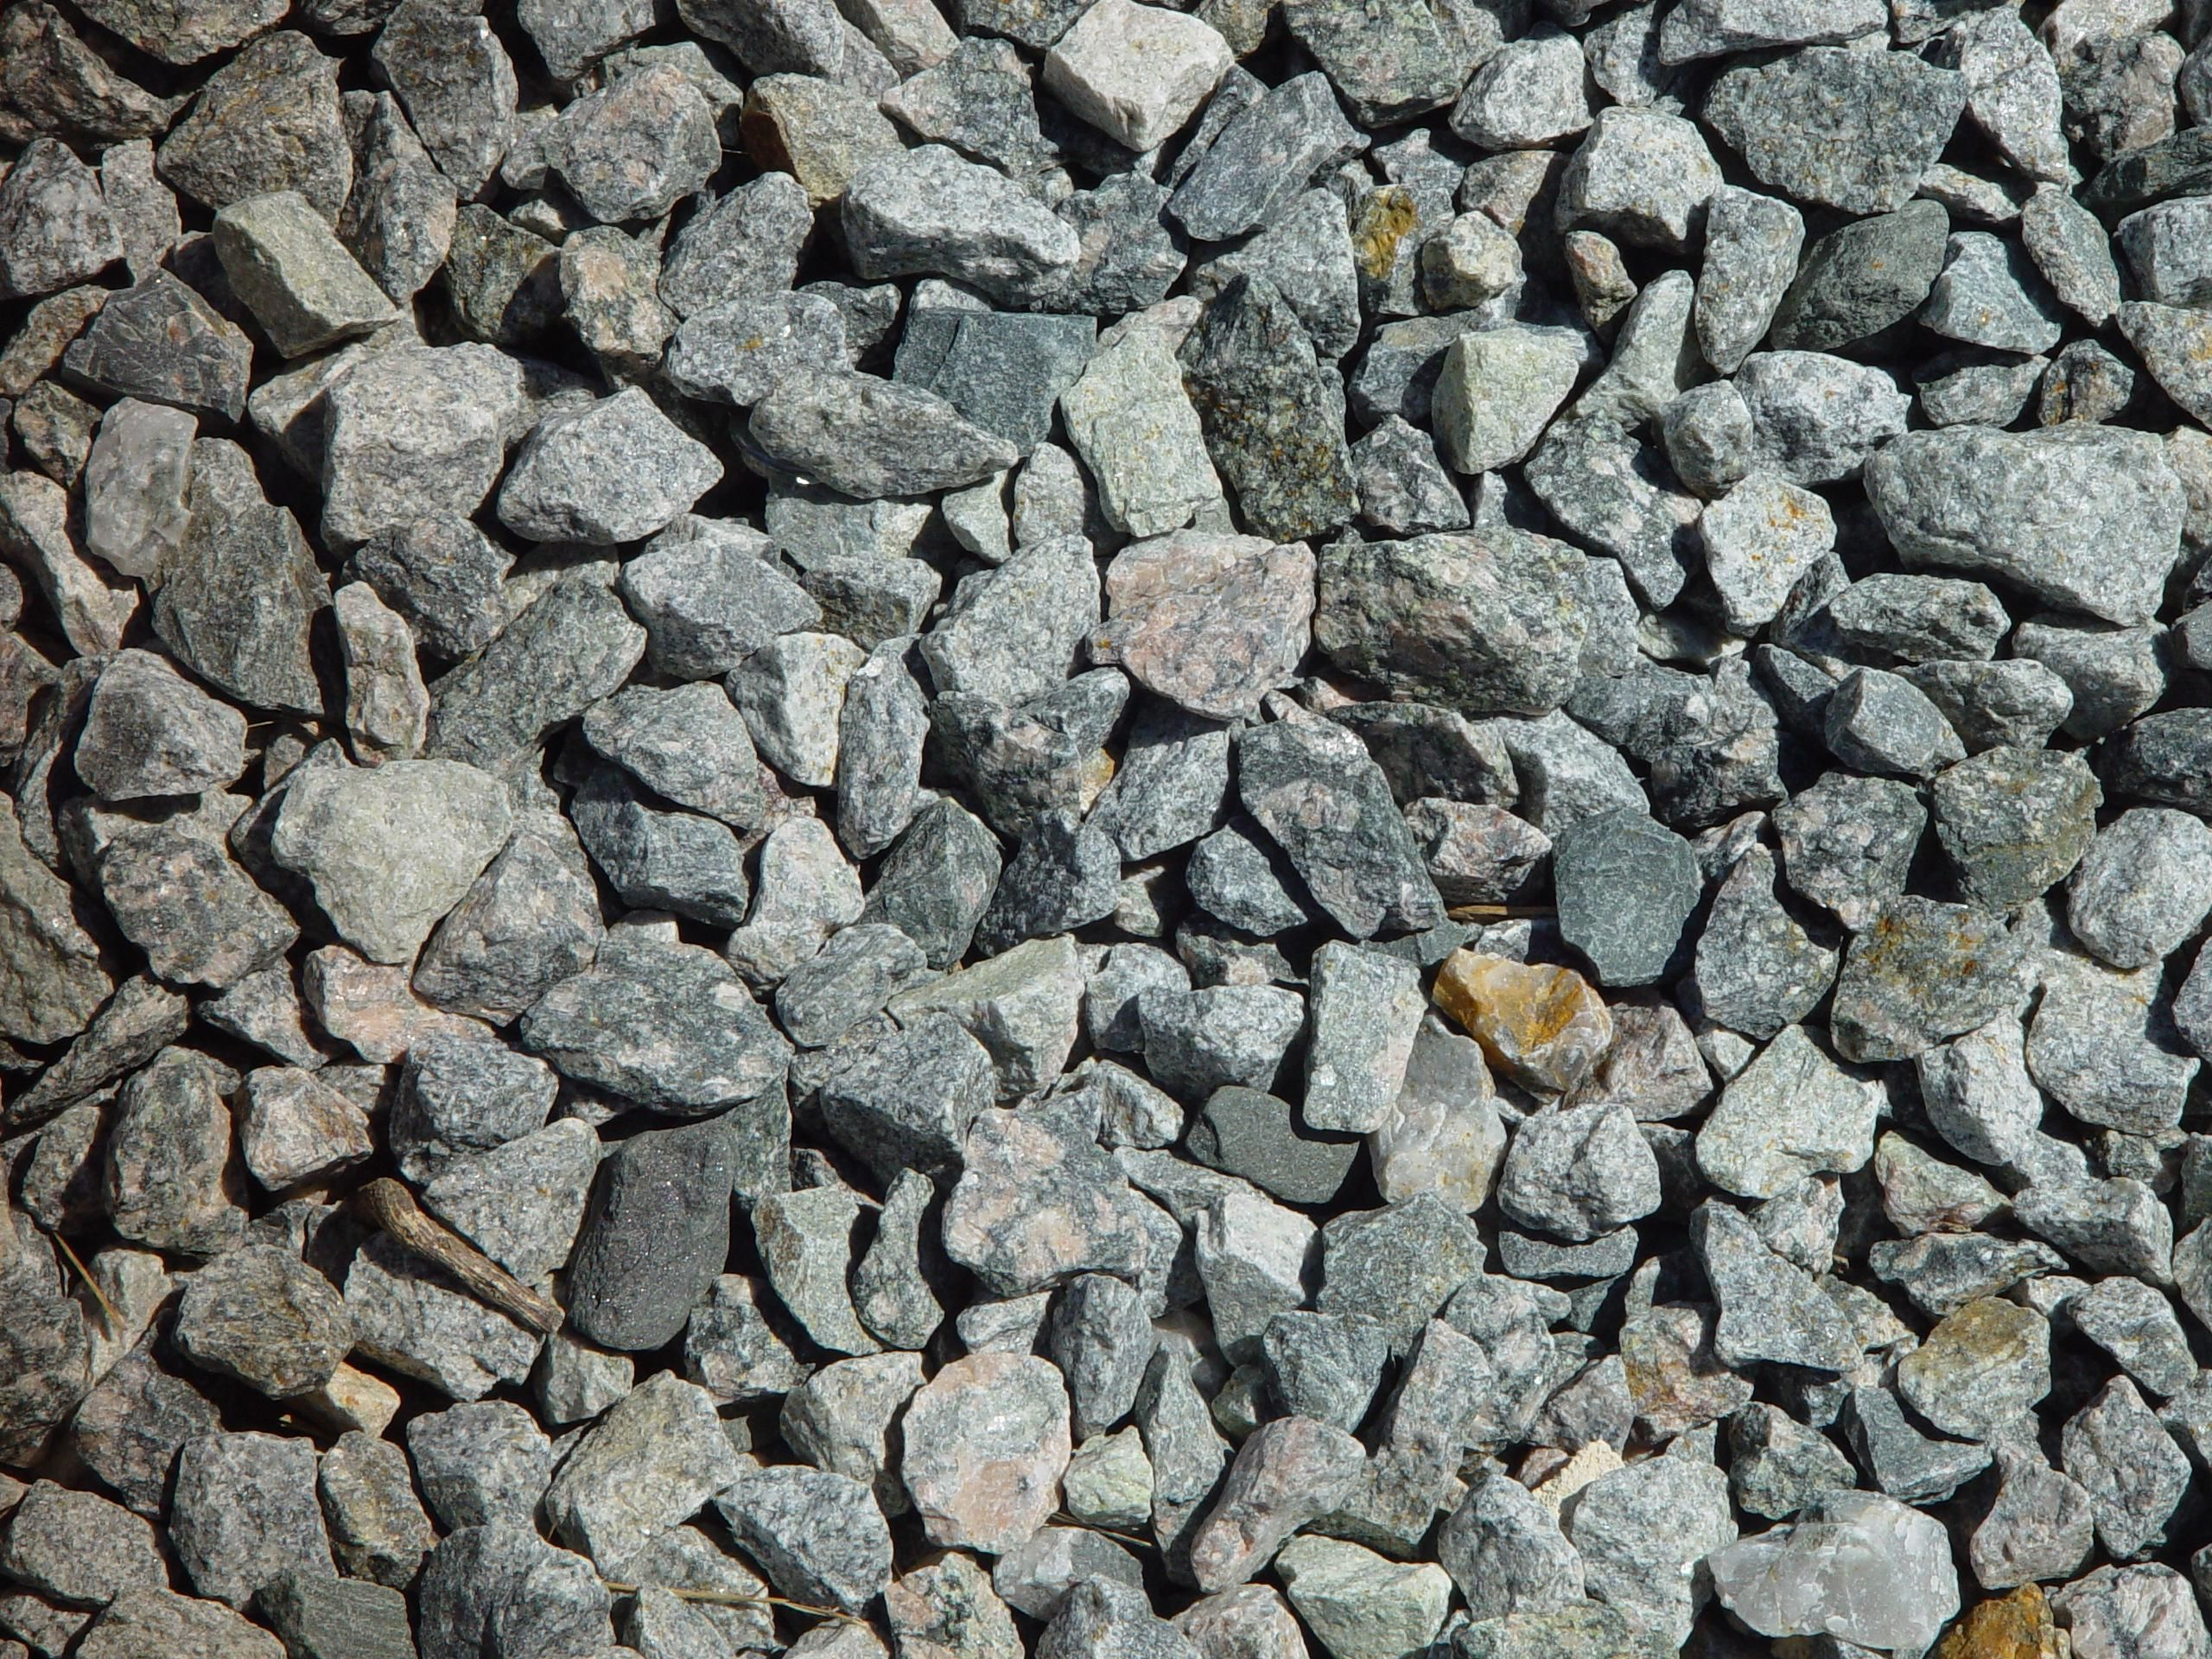
\includegraphics[width=.50\columnwidth]{images/133gravel}
\caption[Gravel]{Gravel.}
\label{fig:133gravel}
\end{figure}
\begin{figure}[!htb]
\centering
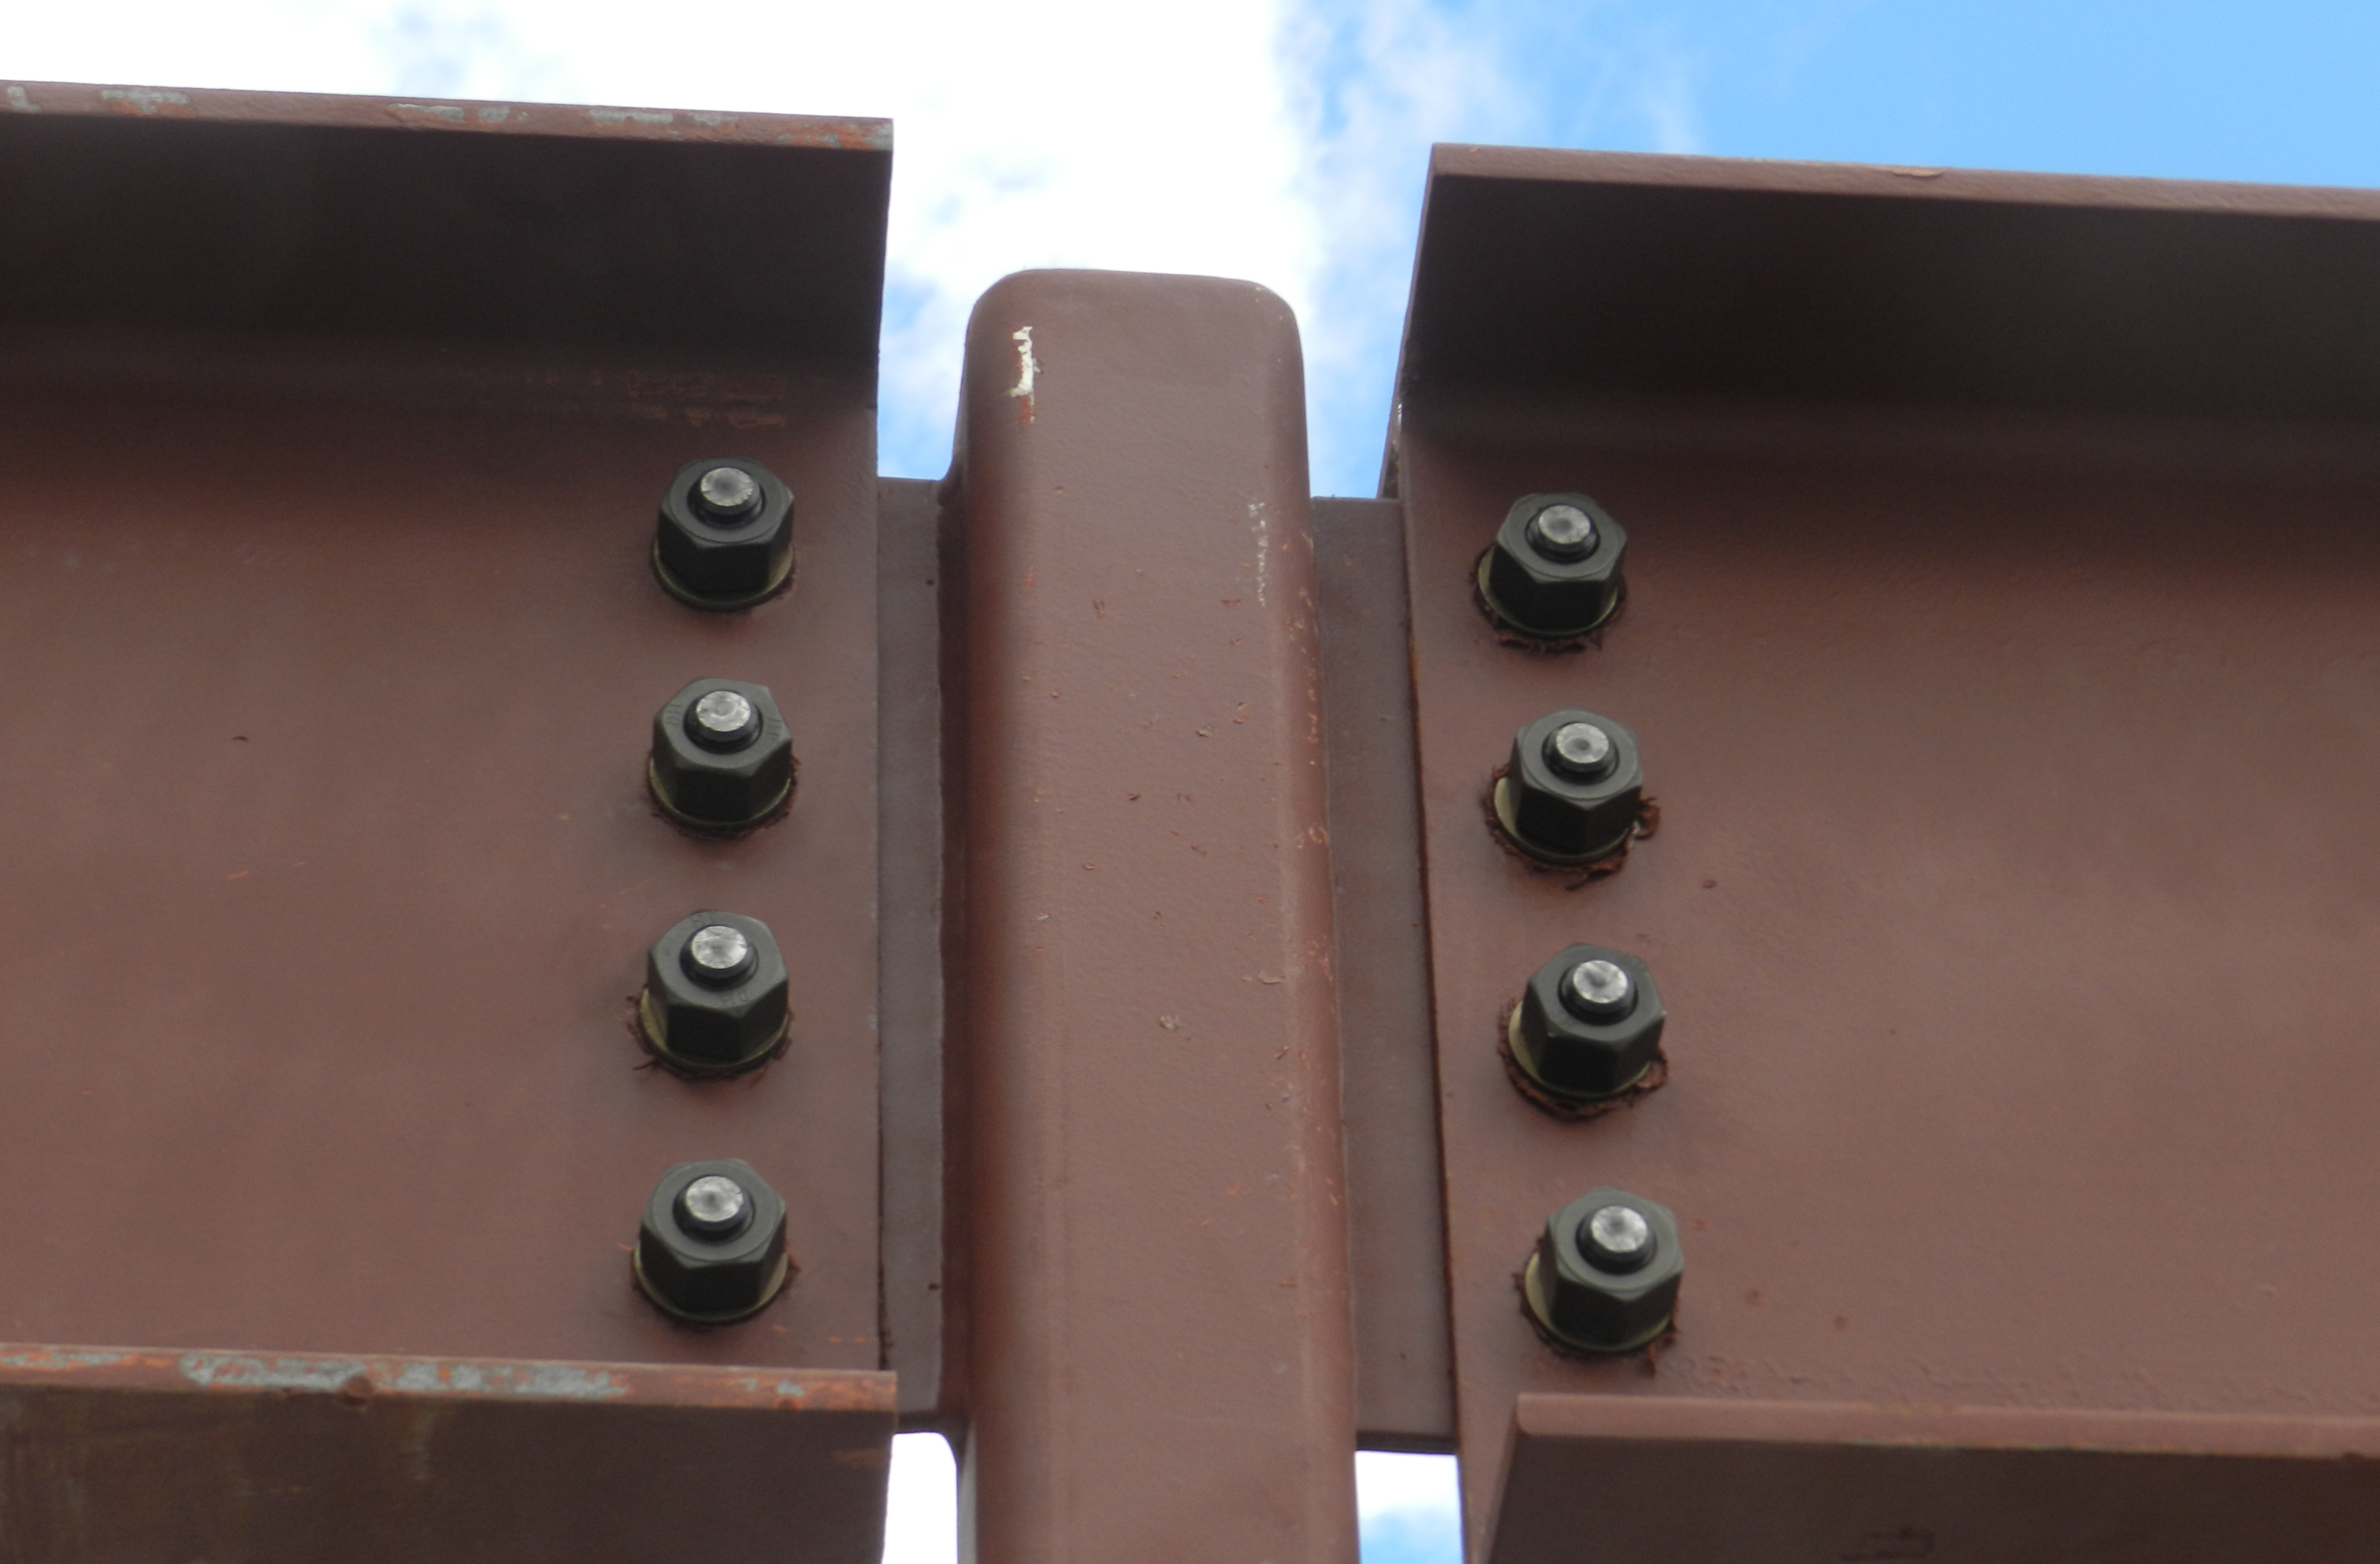
\includegraphics[width=.50\columnwidth]{images/050steel}
\caption[Steel]{Steel.}
\label{fig:050steel}
\end{figure}
In fact, gravels, Fig. \ref{fig:054bsgmaterials}, or granular particles in
general, are far from being a well-defined and easy to characterize material,
for instance a steel beam, Fig.
\ref{fig:050steel}. For continuous materials simulation
parameters are readily available.
In case of a pile of particles the sum of discrete particle properties determines the pile's macroscopic behavior 
(e.g. angle of repose).
In discrete particle simulations particle based parameters (e.g. contact parameters) determine the macroscopic behavior 
of the ensemble.
Unfortunately, particles are not uniform and particle based simulation
parameters are difficult to obtain, and also depends on the numerical shape
(polyhedral, multi-spheres, and simple spheres).
A set of experimental and numerical solutions, together with artificial neural networks, can improve the accuracy 
and the range of applicability of the characterization of particles properties, and reduce the computational costs.
Discrete Element Method requires parameters for the individual contact, but characterize every particle is prohibitive.
We need to find average contact parameters that lead to the expected bulk effect.
We could start with an example of piled particles, more specifically called the
drained angle of repose. This angle of repose \ref{fig:060aor},
characteristic of the bulk macroscopic behaviour of the ensemble, is originated from the microscopic
characteristics of each particle.
\begin{figure}[htbp]
  %\null\hfill
  \subfloat[Silibeads angle of repose.]{
	  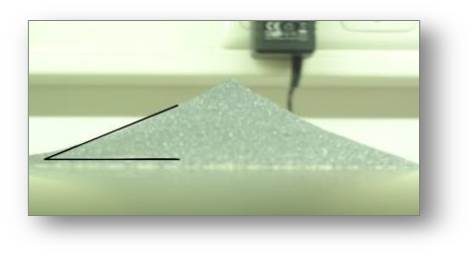
\includegraphics[width=.48\columnwidth]{images/058silibeads}
	  \label{fig:058silibeads}
  }
  \quad
 % \hfill
  \subfloat[Sinter pellets  angle of repose.]{
	  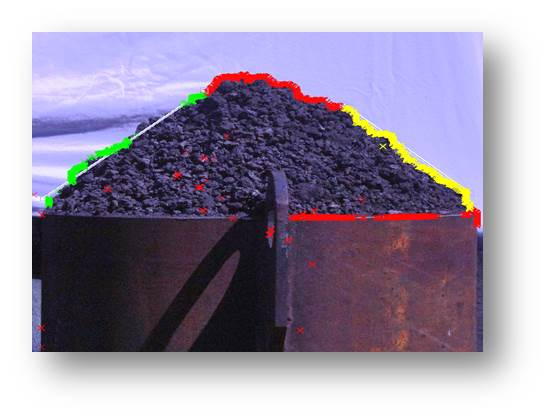
\includegraphics[width=.48\columnwidth]{images/059sinterpellets}
	  \label{fig:059sinterpellets}
  }
 % \hfill\null
  \caption{Angle of repose identification.}
  \label{fig:060aor}
\end{figure}
Measurement of a bulk parameter value, through calibration we obtain the
individual contact parameters:
\begin{enumerate}
\item{Chose initial set of parameters}
\item{DEM simulation}
\item{Compare macroscopic DEM simulation results with experiments}
\item{Choose new parameters}
\end{enumerate}
By our calibration procedure we obtain valid sets of particle based simulation parameters.
Ok, but that's very time consuming, because in each control loop we have to
perform a complete $DEM$ simulation in our case we would need 9.900 days on a 32
core machine. It is not necessary to evaluate a huge number of parameter sets,
rather we should try to evaluate the \textbf{sensitivity} 
of the macroscopic bulk behavior with respect to individual particle based parameters.
This can be realized efficiently by artificial neural networks Fig.
\ref{fig:048neuron0}!
\improvement{few words on biological relationship}
\begin{figure}[!htb]
\centering
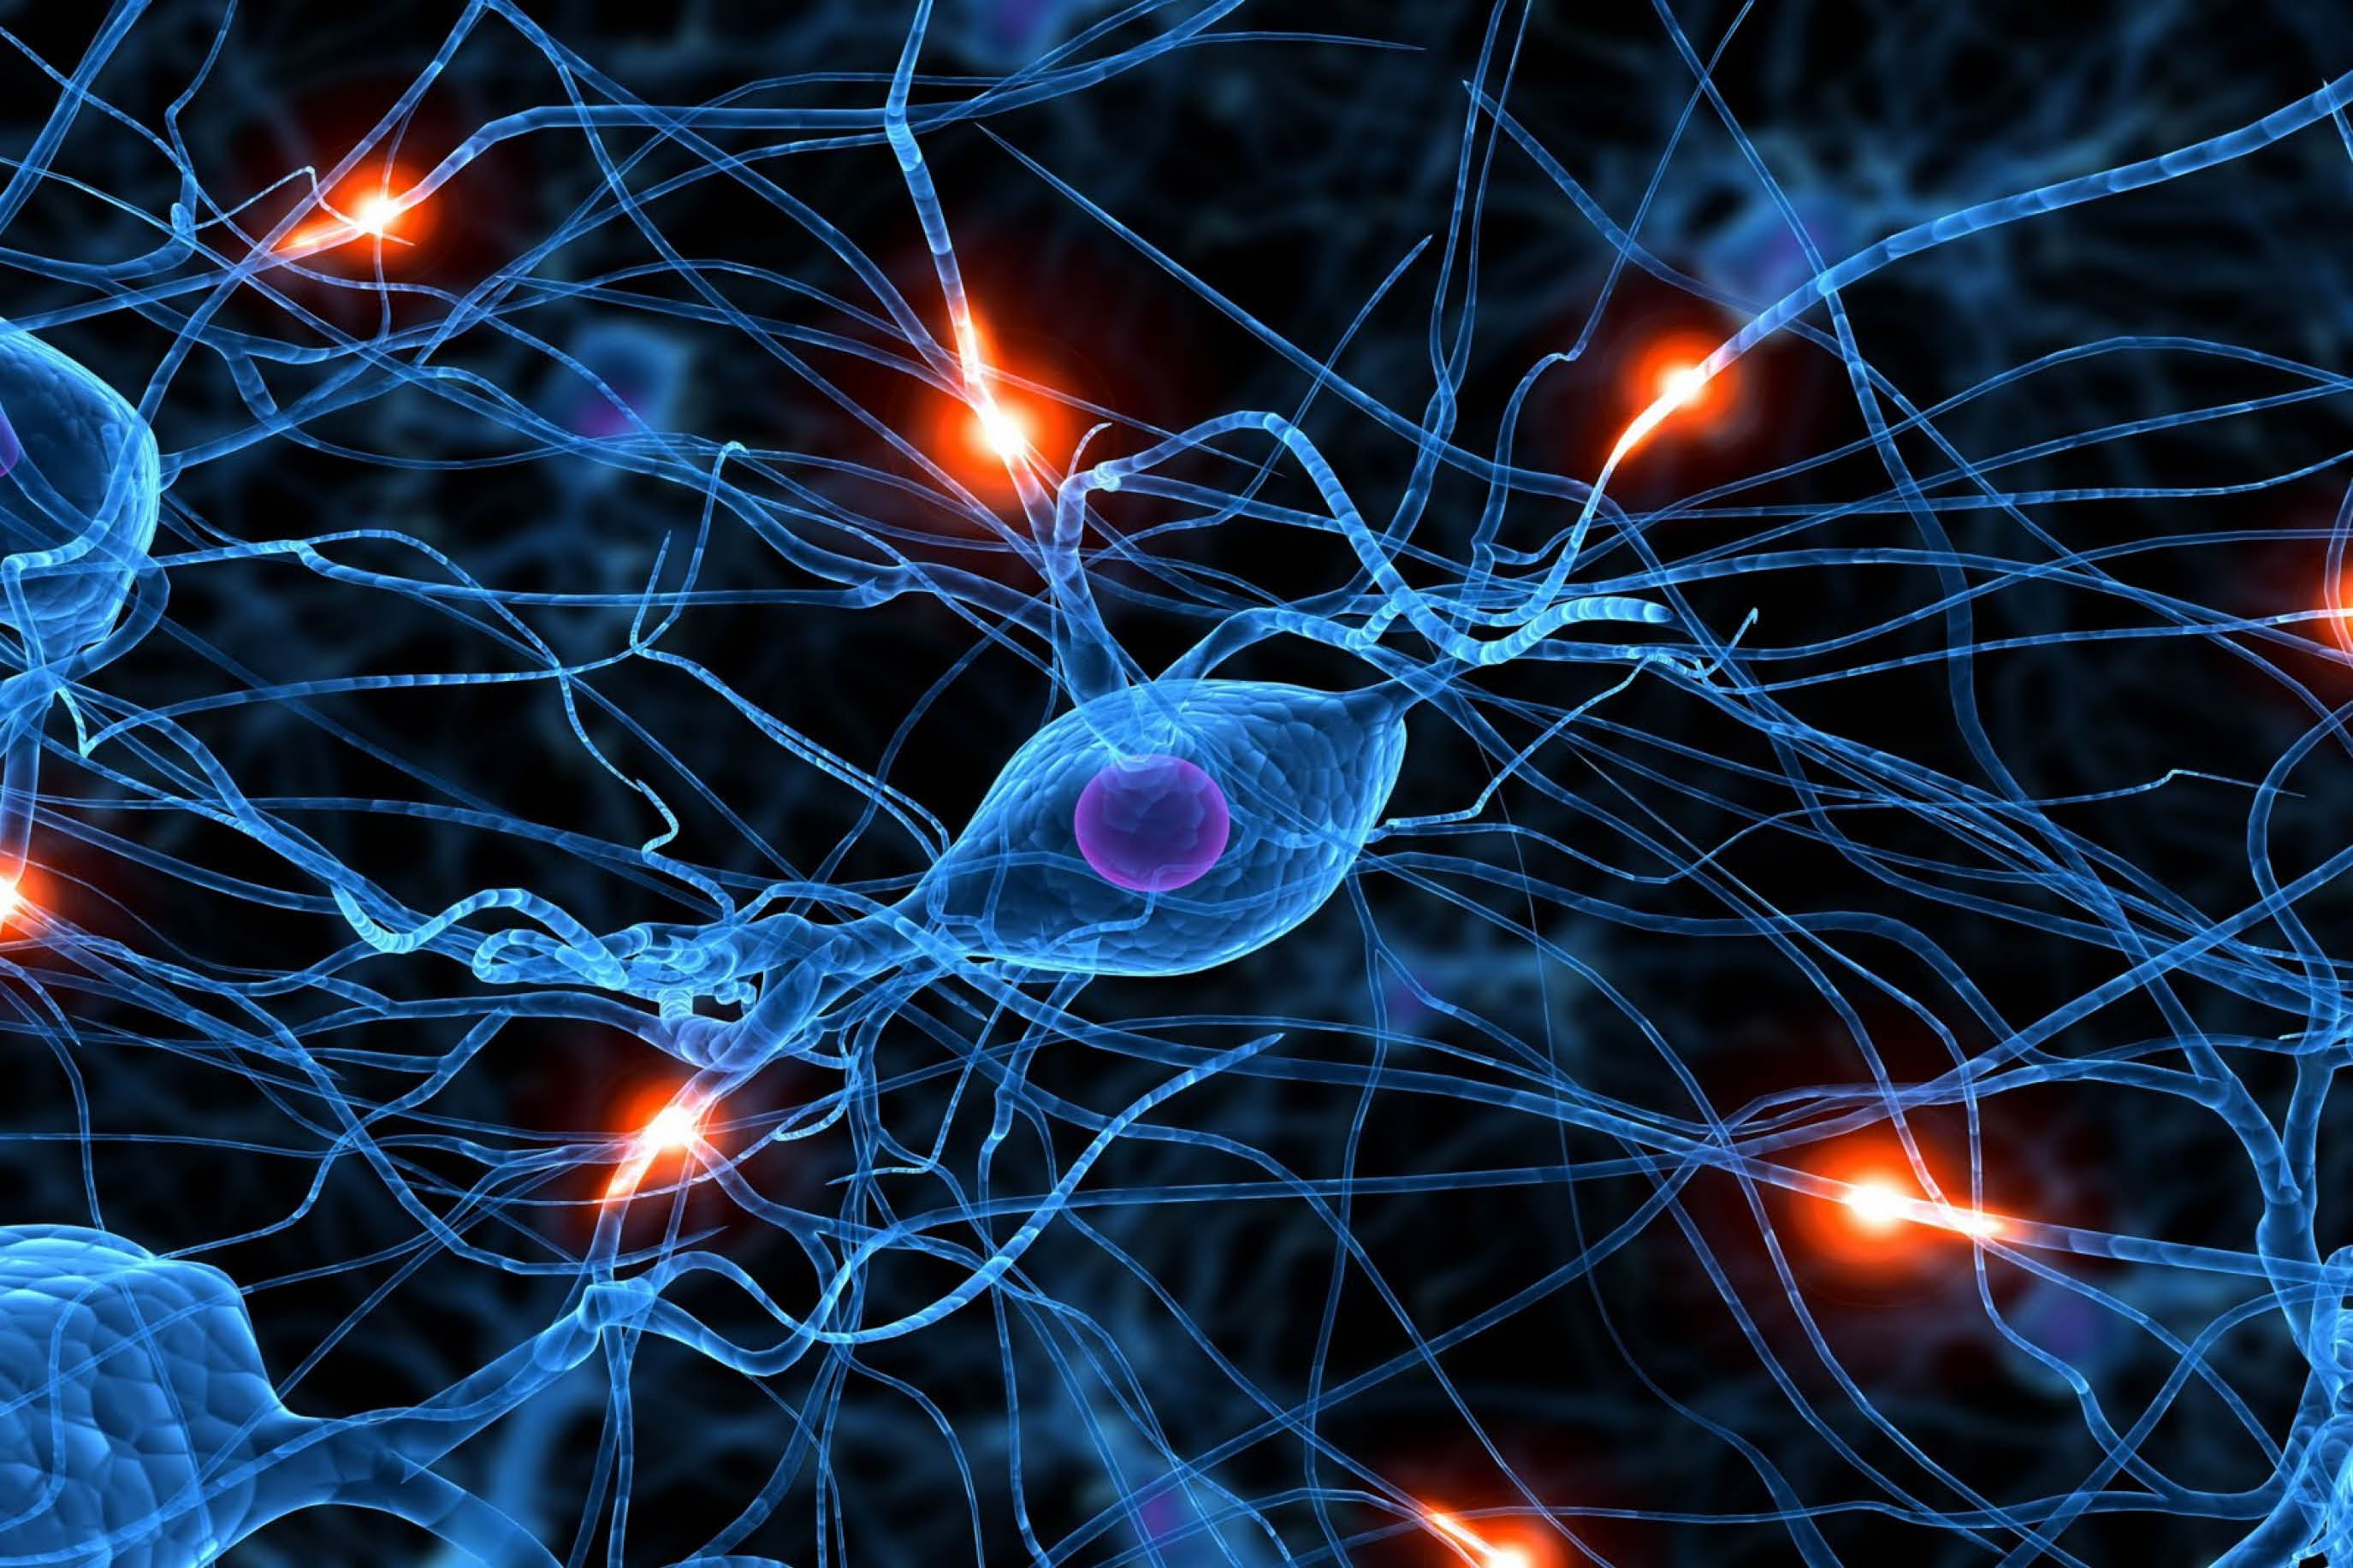
\includegraphics[width=.50\columnwidth]{images/048neuron0}
\caption[Biological inspiration]{Biological inspiration for the Artificial
Neural Networks: a human neuron with the incoming electric signals
\cite{RefWorks:158}.}
\label{fig:048neuron0}
\end{figure}
In this artificial neural network neurons are linked to particle based input parameters. 
By matching the output of the artificial neural network to DEM simulation results the network is trained 
(i.e. individual neurons are weighted).
Later, the trained neural network can be used to predict additional valid sets of particle based simulation parameters. 

\begin{enumerate}
\item{Train neural network by 500 dedicated DEM simulations (time consuming)}
\item{Test another 6.250.000 combinations by the neural network (very fast)}
\item{Check if predictions of neural network are correct (by comparing with experimental  values)}
\end{enumerate}

Typically, less than 1\% of the tested parameter sets lead to correct
macroscopic results (i.e. 6.000 to 60.000 valid parameter sets).
By this assessment of particle based simulation parameters we obtain valuable information about the dependence 
of bulk solid behavior on individual particle properties.
First we can determine the validity range, mean and variance band of each input
parameter. Next we can determine a probability density function for each input
parameter. Then, we can investigate mutual dependencies.
This calibration procedure is universal in a sense that the same artificial neural network can be harnessed for 
different macroscopic bulk behaviors.
This effort is really necessary because the predictive capability of any DEM simulation strongly 
depends on the validity of the particle 
based simulation parameters.
\improvement{add some words on the applications}

% !TEX encoding = UTF-8
% !TEX TS-program = pdflatex
% !TEX root = ../Tesi.tex
% !TEX spellcheck = en-EN

%************************************************
\chapter{Prologue}
\label{cap:prologue}
%************************************************

Particles in various forms - ranging from raw materials to food grains and pharmaceutical powders - 
play a major role in a variety of industries, including process industry and metallurgy. 
In his book, \citet{RefWorks:117} stated that "between 1 and 10\% of all the energy is used in 
comminution, i.e. the processes of crushing, grinding, milling, micronising". 
Many methods have been developed to study particles.
For instance, Discrete Element Methods (\acs{DEMs}), "a special class of numerical
schemes for simulating the behavior of discrete, interacting bodies", are widely used to 
simulate particle behaviour in these granular processes
(\citet{RefWorks:130}).\\ 

\section{Metallurgical industry}
\label{sec:metallurgical industry}
In this thesis, we focused on the granular materials the metallurgical industry
handles, especially, in two processes:
\begin{itemize}
  \item{sinter cooling,}
  \item{pig ore smelting through a blast furnace.} 
\end{itemize} 

In the first process we were interested about a sinter chute
segregator, or more specifically, about the size distribution of the particles
at its exit.\\
In the second process, we wanted to investigate the raceway zone of the blast
furnace, both its formation and its evolution.

\section{Challenges}
\label{sec:challenges}

\begin{figure}[!htb]
\centering
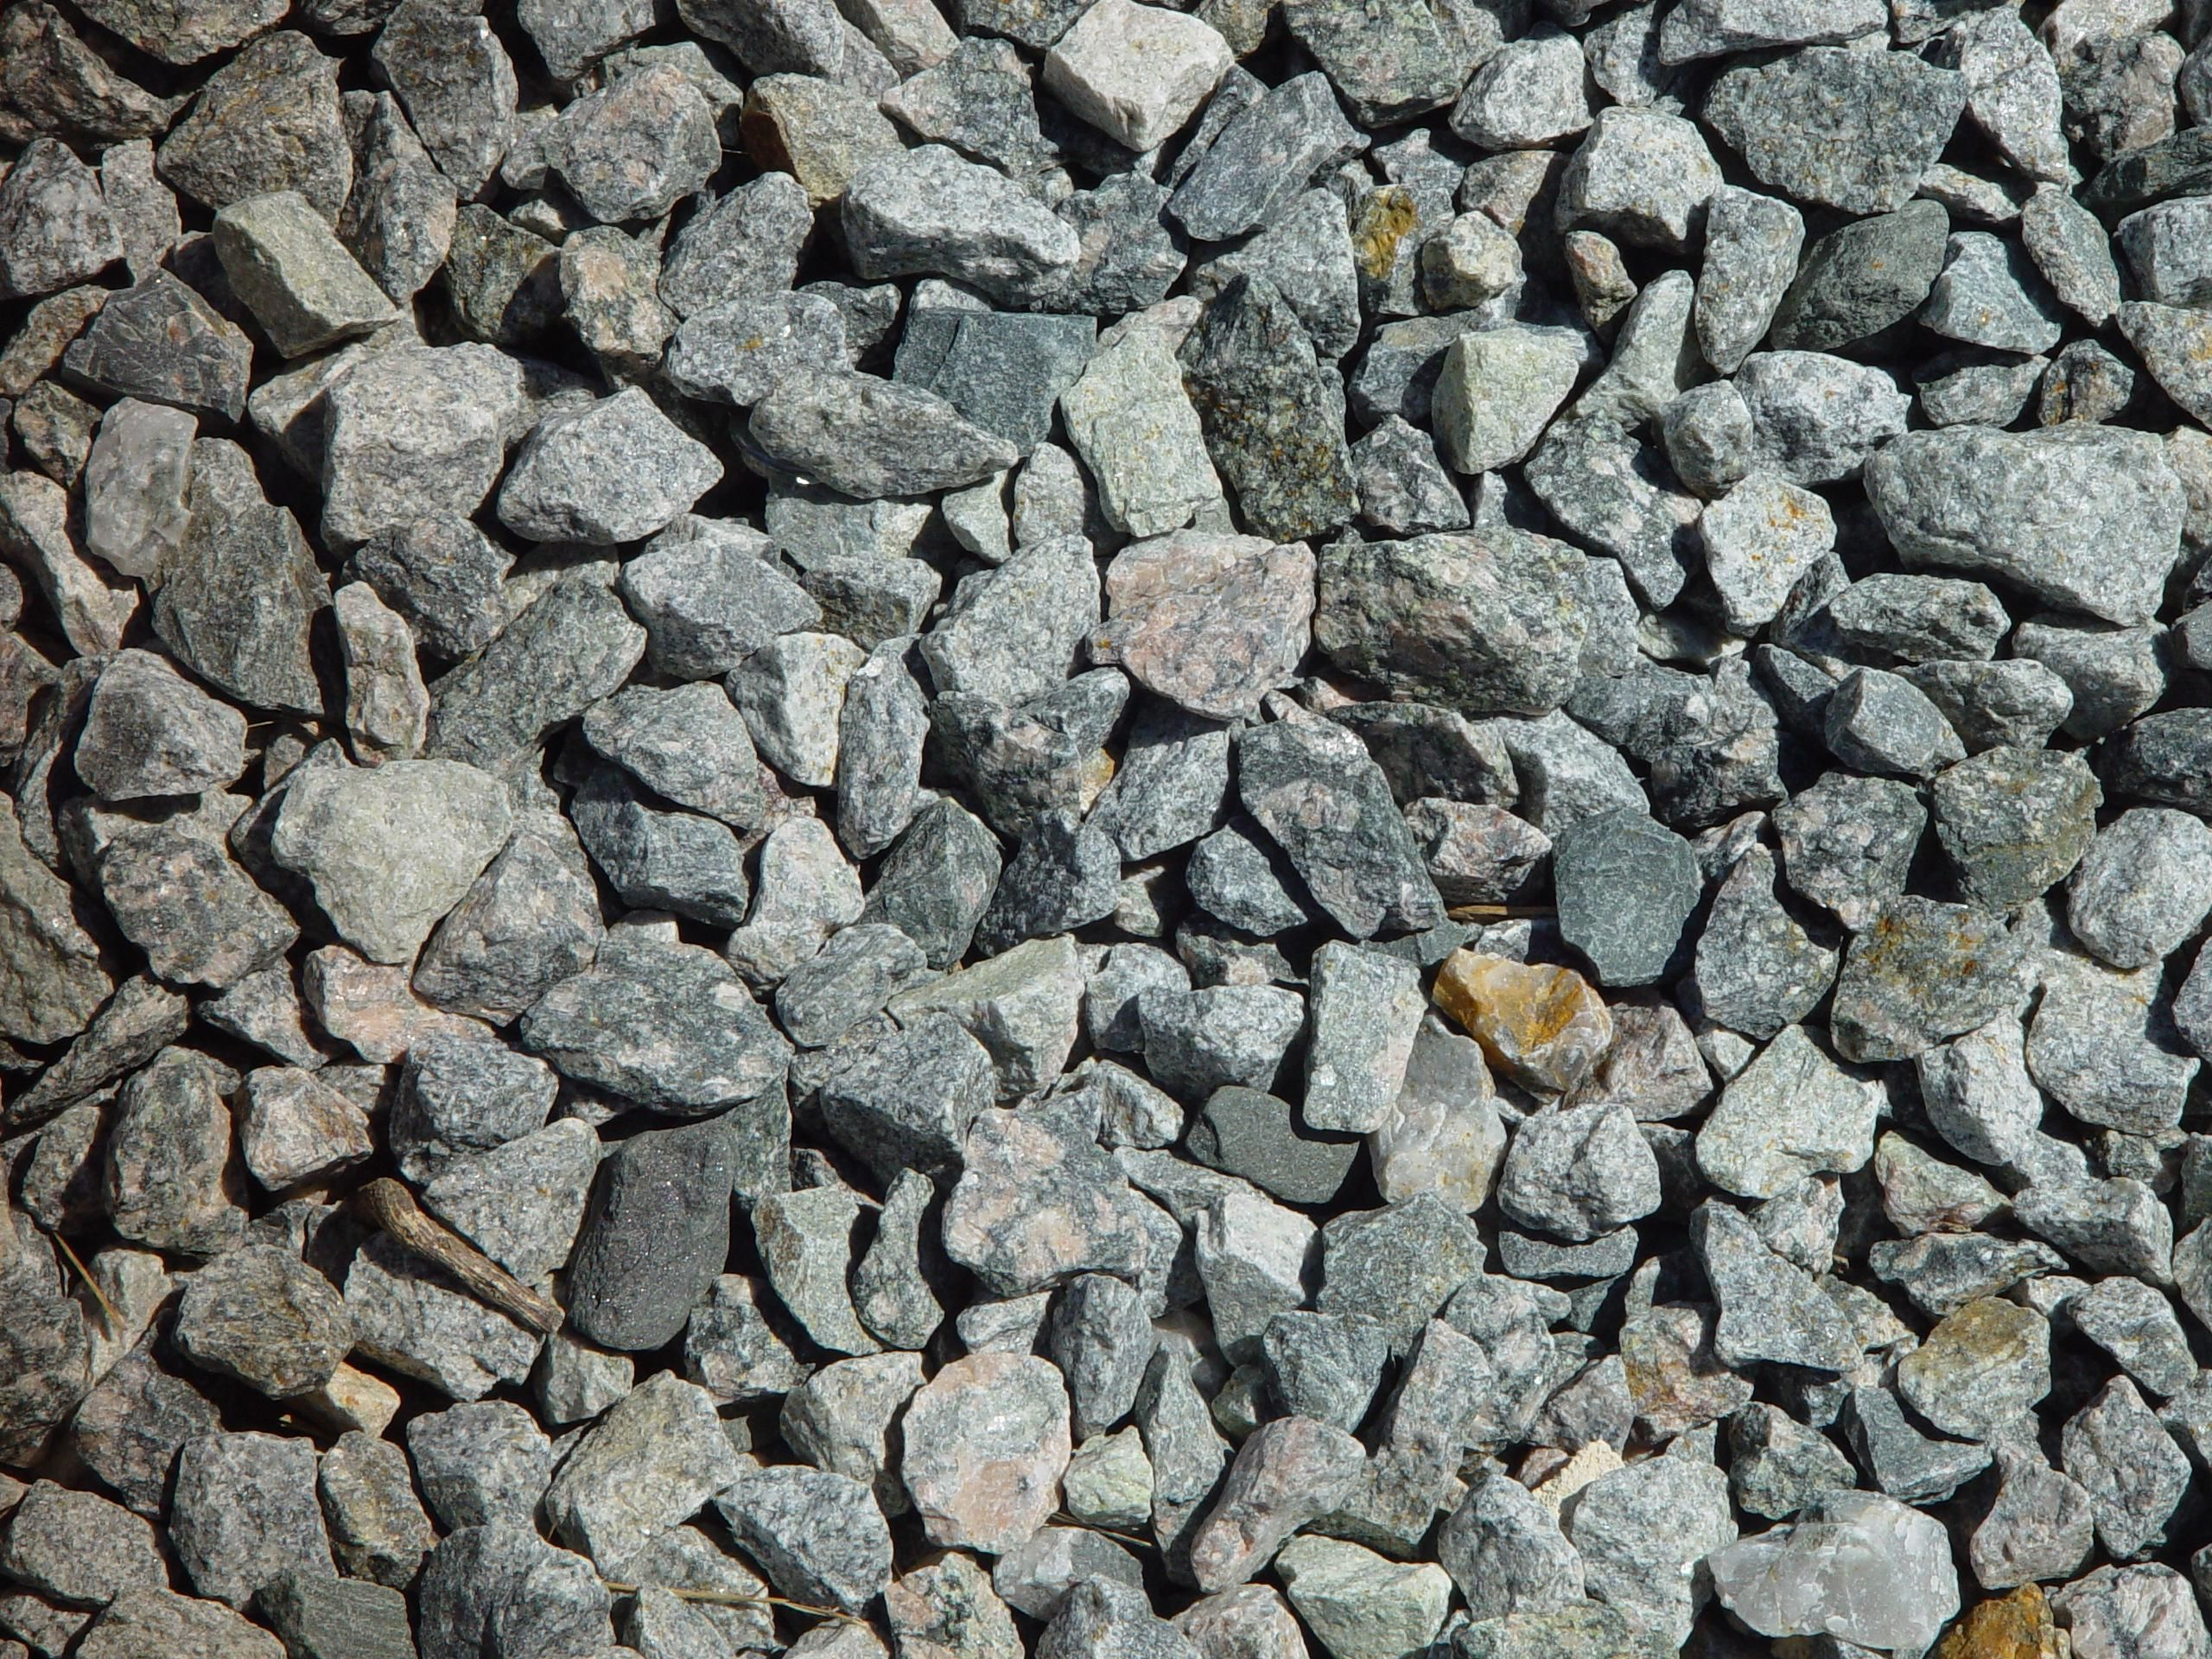
\includegraphics[width=.50\columnwidth]{images/133gravel}
\caption[Gravel]{Gravel.}
\label{fig:133gravel}
\end{figure}
\begin{figure}[!htb]
\centering
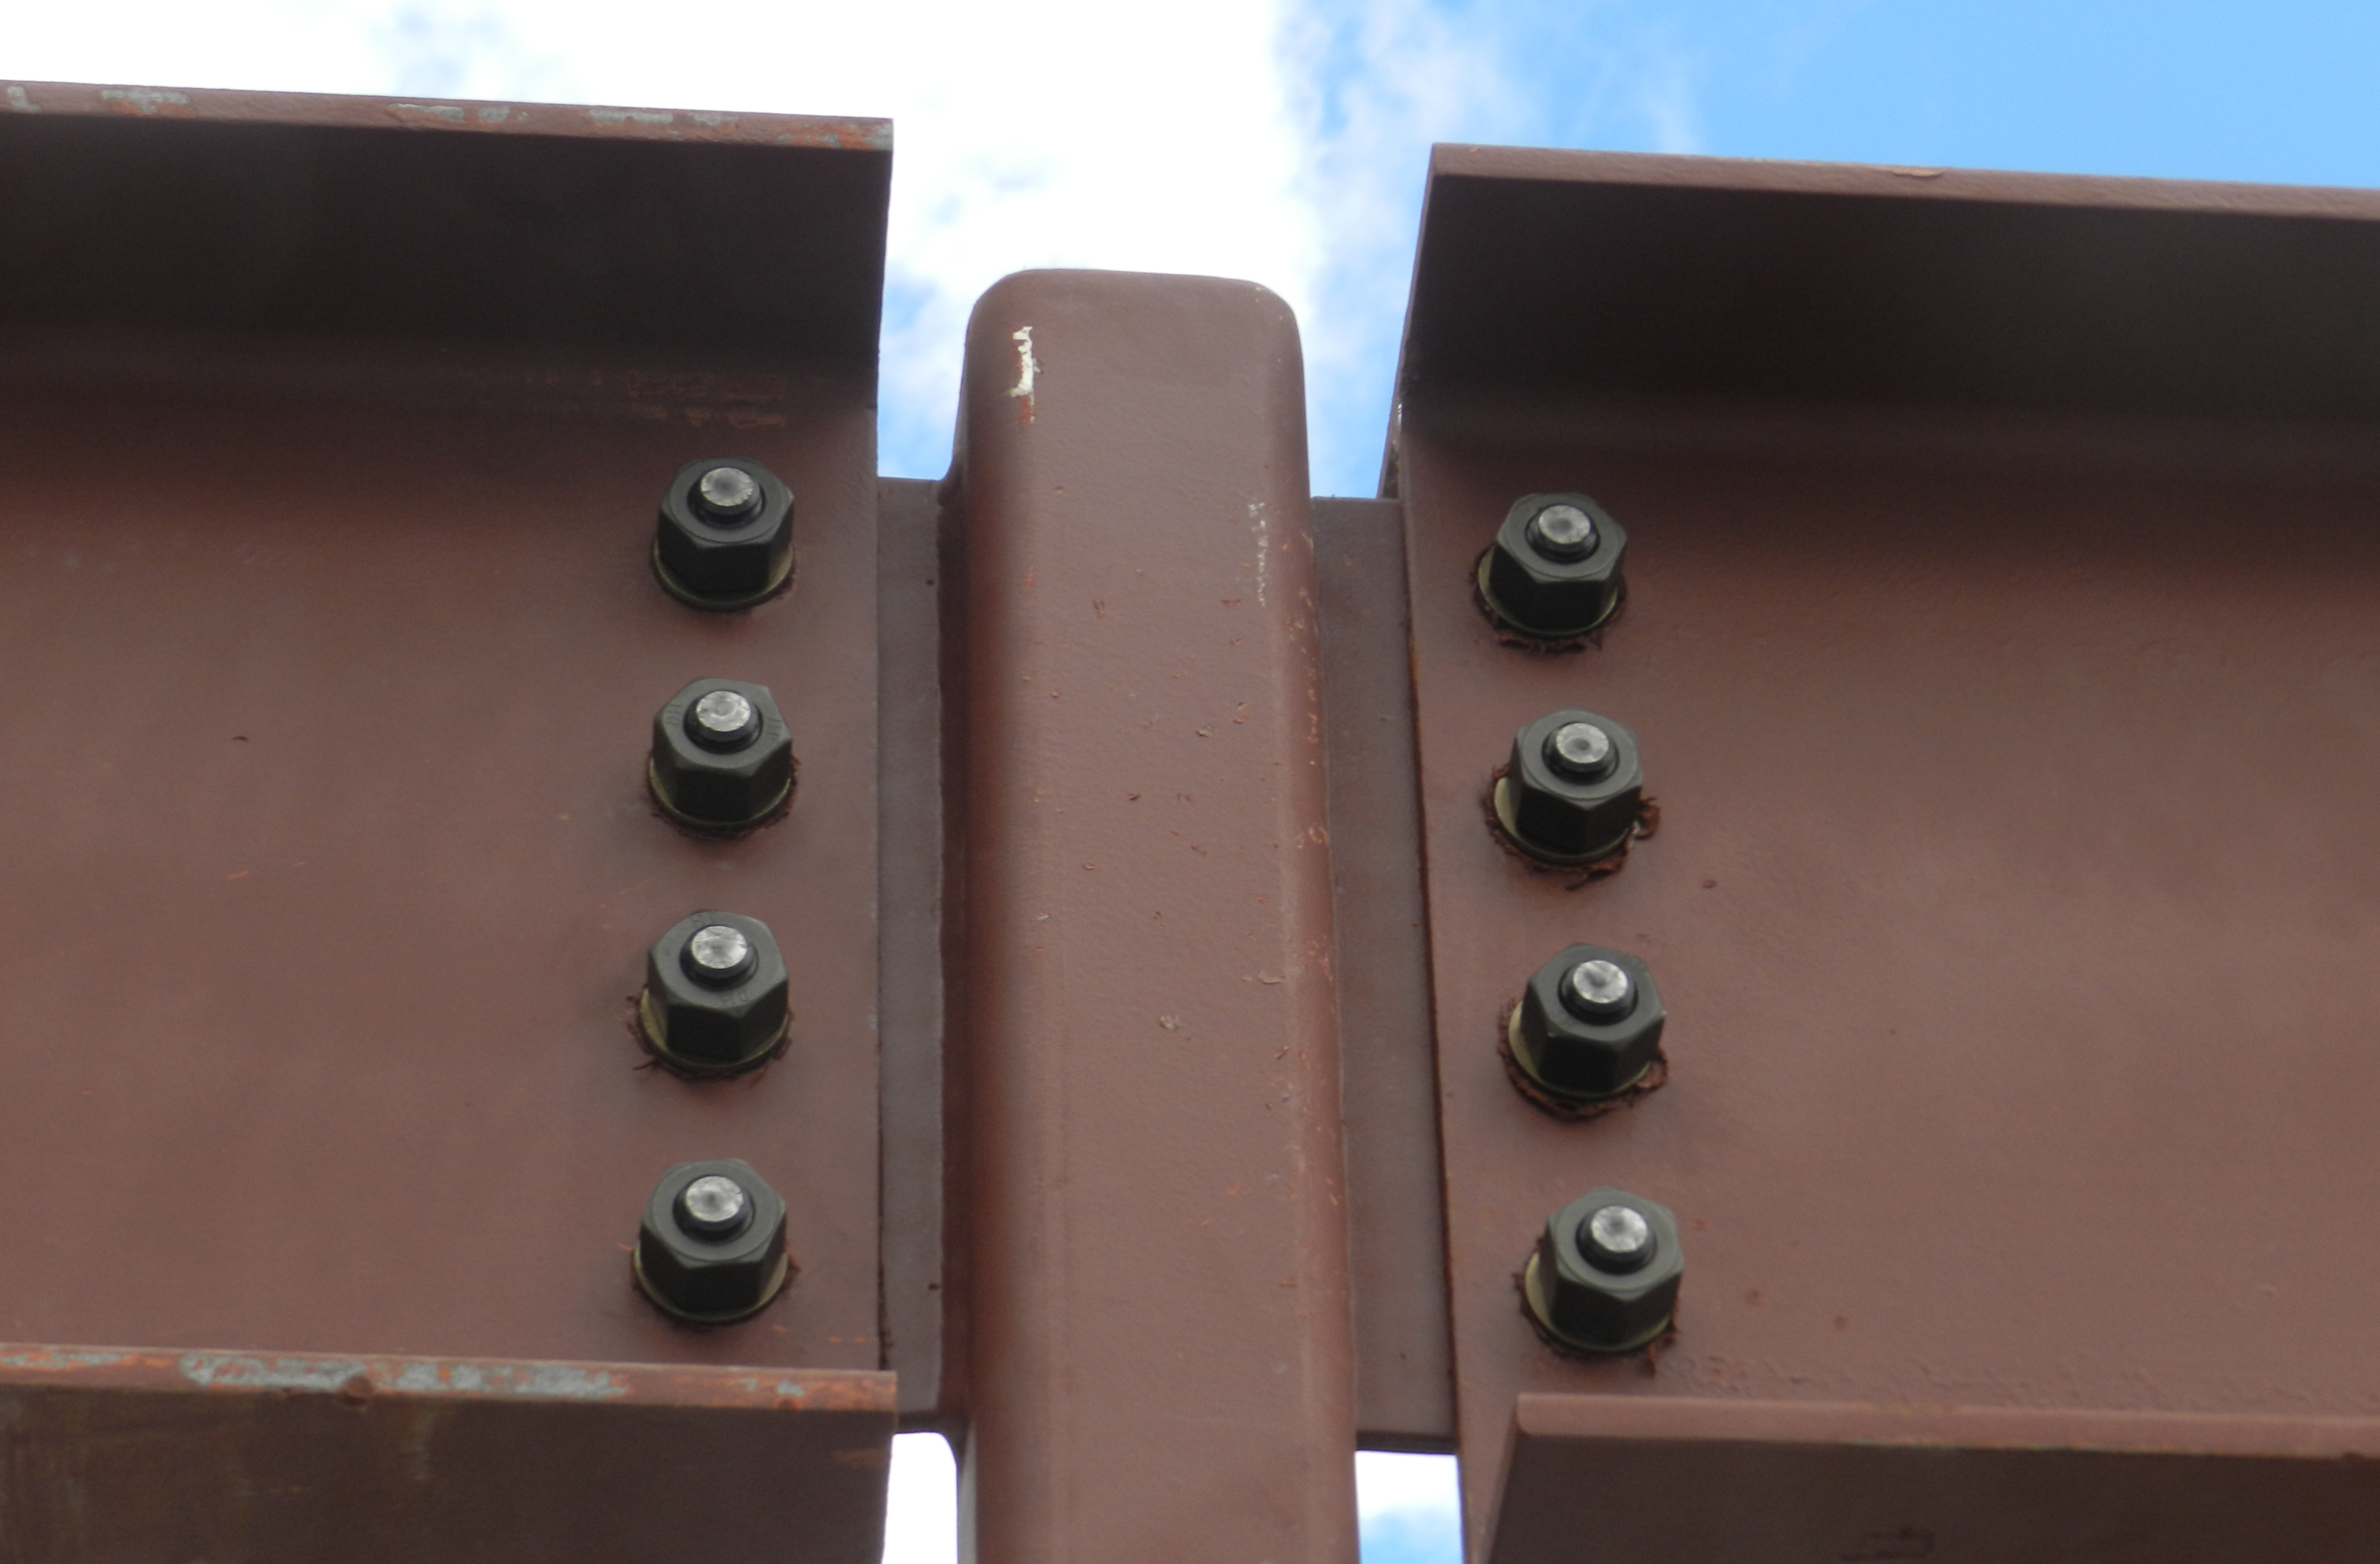
\includegraphics[width=.50\columnwidth]{images/050steel}
\caption[Steel]{Steel.}
\label{fig:050steel}
\end{figure}
In fact, gravels, Fig. \ref{fig:054bsgmaterials}, or granular particles in
general, are far from being a well-defined and easy to characterize material,
like for instance a steel beam, Fig.
\ref{fig:050steel}. For continuous materials simulation
parameters are readily available.
In case of a pile of particles the sum of discrete particle properties determines the pile's macroscopic behavior 
(e.g., angle of repose).\\
In discrete particle simulations particle based parameters (e.g., contact
parameters) determine the macroscopic behavior of the ensemble.
Unfortunately, particles are not uniform and particle based simulation
parameters are difficult to obtain, and also depends on the numerical shape
(polyhedral, multi-spheres, and simple spheres).

\section{Calibration}
\label{sec:calibration}

A set of experimental and numerical solutions, together with artificial neural
networks to regress the inverse problem, could improve the accuracy and the
range of applicability of the characterization of particles properties, and reduce the computational costs.
The Discrete Element Method requires parameters for the individual contact, but
to characterize every particle is prohibitive.\\
We needed to find average contact parameters that could lead to the expected
bulk effect.
We could start with an example of piled particles, more specifically called the
drained angle of repose. This angle of repose, see Fig. \ref{fig:060aor},
characteristic of the bulk macroscopic behaviour of the ensemble, is originated from the microscopic
characteristics of each particle.
\begin{figure}[htbp]
  %\null\hfill
  \subfloat[Silibeads angle of repose.]{
	  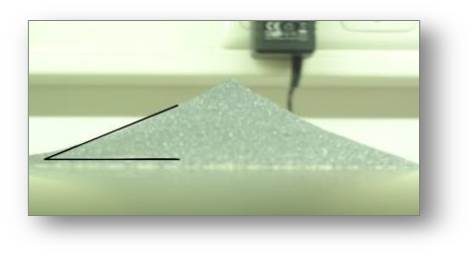
\includegraphics[width=.48\columnwidth]{images/058silibeads}
	  \label{fig:058silibeads}
  }
  \quad
 % \hfill
  \subfloat[Sinter pellets  angle of repose.]{
	  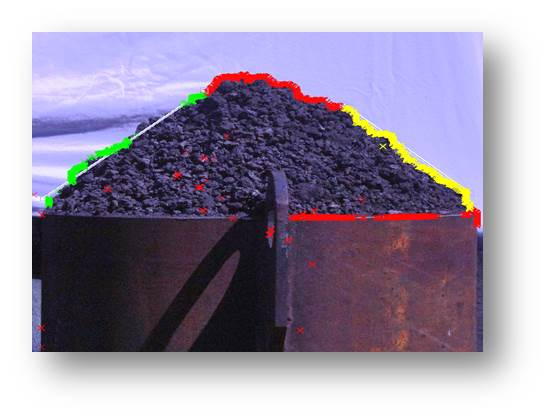
\includegraphics[width=.48\columnwidth]{images/059sinterpellets}
	  \label{fig:059sinterpellets}
  }
 % \hfill\null
  \caption{Angle of repose identification.}
  \label{fig:060aor}
\end{figure}
Once measured the bulk parameter value, through calibration we could obtain the
individual contact parameters:
\begin{enumerate}
\item{we chose initial set of parameters;}
\item{we performed a \acs{DEM} simulation;}
\item{we compared macroscopic \acs{DEM} simulation results with experiments;}
\item{if they matched we ended the loop, otherwise we started again from 1 with
new parameters.}
\end{enumerate}
By our calibration procedure we could obtain valid sets of particle based
simulation parameters in an extremely time consuming way, because in each
control loop we would have to perform a complete \acs{DEM} simulation.
In fact, a feasibility study from \citet{RefWorks:173}
required a total of
9.900 days on a 32 core machine to reliably complete a calibration procedure.
However, the evaluation of a a large number of parameter sets can not be
considered essential, nor necessary. 
Our aim was rather to determine the \textit{sensitivity} 
of the macroscopic bulk behavior with respect to individual particle based parameters.
This could be realized efficiently by artificial neural networks, see Fig.
\ref{fig:048neuron0}. 

\section{Neural Network Calibration}
\label{sec:neuralnetworkcalibration}

After the original work of \citet{RefWorks:189} we know that the human brain is
composed of neurons and their connections. 
They receive inputs from receptive
nerves and together elaborate an output response (e.g., to remove the hand from
a hot surface).
\begin{figure}[!htb]
\centering
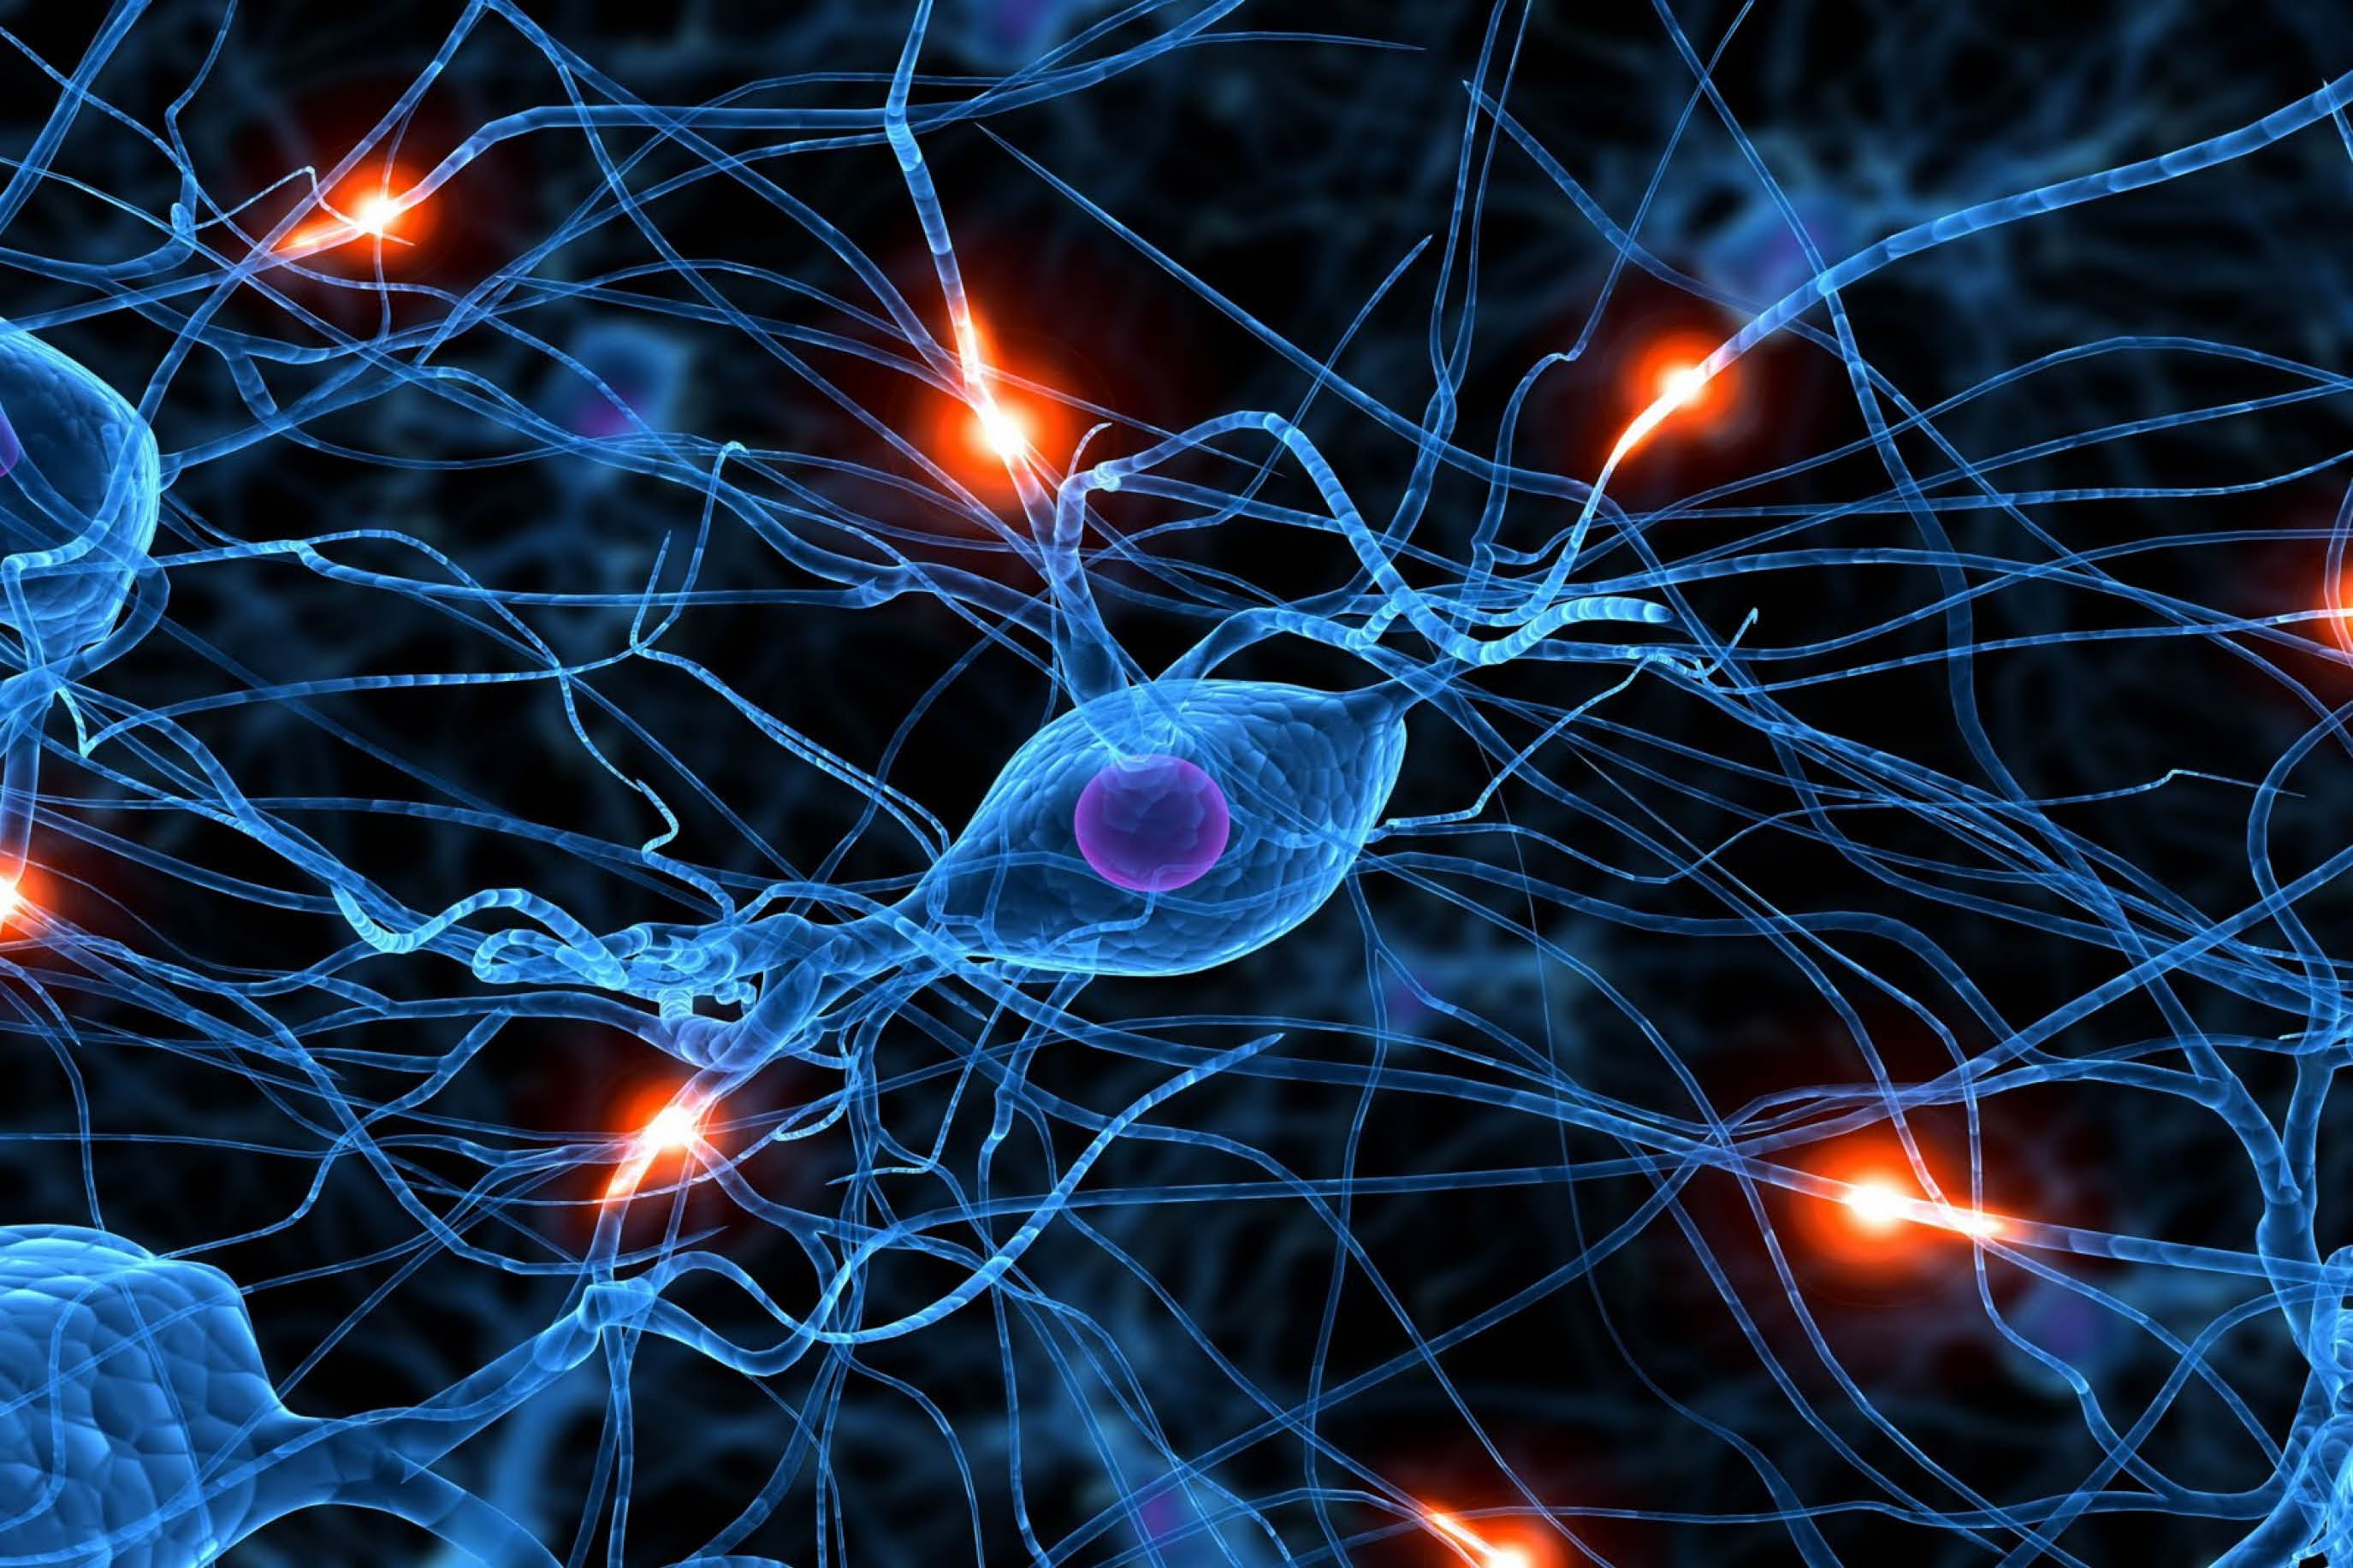
\includegraphics[width=.50\columnwidth]{images/048neuron0}
\caption[Biological inspiration]{Biological inspiration for the Artificial
Neural Networks: a human neuron with the incoming electric signals
\cite{RefWorks:158}.}
\label{fig:048neuron0}
\end{figure}
Similarly, in the artificial neural network we trained a series of neurons to
solve a regression problem.
The neurons had
as inputs particle based parameters and as output the corresponding \acs{DEM}
simulation results.
With both data the network was trained (i.e. individual neurons are
weighted).
Later, the trained neural network could be used to predict additional valid sets
of particle based simulation parameters.

\begin{enumerate}
\item{We trained a neural network by approximately 500 dedicated \acs{DEM} simulations
(time consuming);}
\item{we predicted another 6 250 000 combinations by the neural network
(fast);}
\item{we checked the corrrectness of the neural network predictions (by
comparing with experimental  values).}
\end{enumerate}

\section{Parameters Identification}
\label{sec:parametersidentification}

In our experience, less than 1\% of the predicted parameter sets lead to correct
macroscopic results (i.e. 6.000 to 60.000 valid parameter sets).
By this assessment of particle based simulation parameters we obtained valuable
information about the dependence of bulk solid behavior on individual particle properties.
First we could determine the validity range, mean and variance band of each
input parameter. Next we could determine a probability density function for each
input parameter. Then, we could investigate mutual dependencies.
This calibration procedure was universal in a sense that the same artificial
neural network could be harnessed for different macroscopic bulk behaviors.
This effort was really necessary because the predictive capability of any
\acs{DEM} simulation strongly depends on the validity of the particle 
based simulation parameters.\\
Once we had reliable \acs{DEM} parameters, we could use them for large scale \acs{DEM}
simulations.
% \begin{itemize}
% \item{;}
% \item{ of a blast furnace.}
% \end{itemize}
% !TEX encoding = UTF-8
% !TEX TS-program = pdflatex
% !TEX root = ../Tesi.tex
% !TEX spellcheck = en-EN

%************************************************
\chapter{Motivation and Insufficiency of the State of the Art}
\label{cap:insufficiency}
%************************************************

% As already mentioned in \ref{sec:metallurgical industry}, this work focused on
% the particles handled by metallurgical industries.
% \improvement{list of metallurgical processes with particulate materials. E.g.,
% blast furnace is fed with coke and sintered iron ore particles: distribution of
% the feed by the chute, raceway formation} 
% \improvement{More words on motivation:
% industrial processes.
% 1)Ask MB brochure on sinter cooler. 2) Ask TL and CF material on raceway (cite Alice's thesis).} 

\citet{RefWorks:195} states that the iron metal can be obtained by reduction of
iron oxides. The most used apparatus to obtain pig iron is the blast furnace.
Iron oxides are mined from earth crust. 
However, a blast furnace needs particles
ranged between 7 and 25 millimiters \cite{RefWorks:195}.
To reach the required specification, the extracted minerals are crushed and then
sieved. Sieving divides the particles in two categories:
\begin{itemize}
  \item{lump ore, between 7 and 25 millimiters,}
  \item{fines, less than 7 millimiters.} 
\end{itemize}

Lump ore can be used directly for blast furnace smelting.\\
\begin{figure}[!htb]
\centering
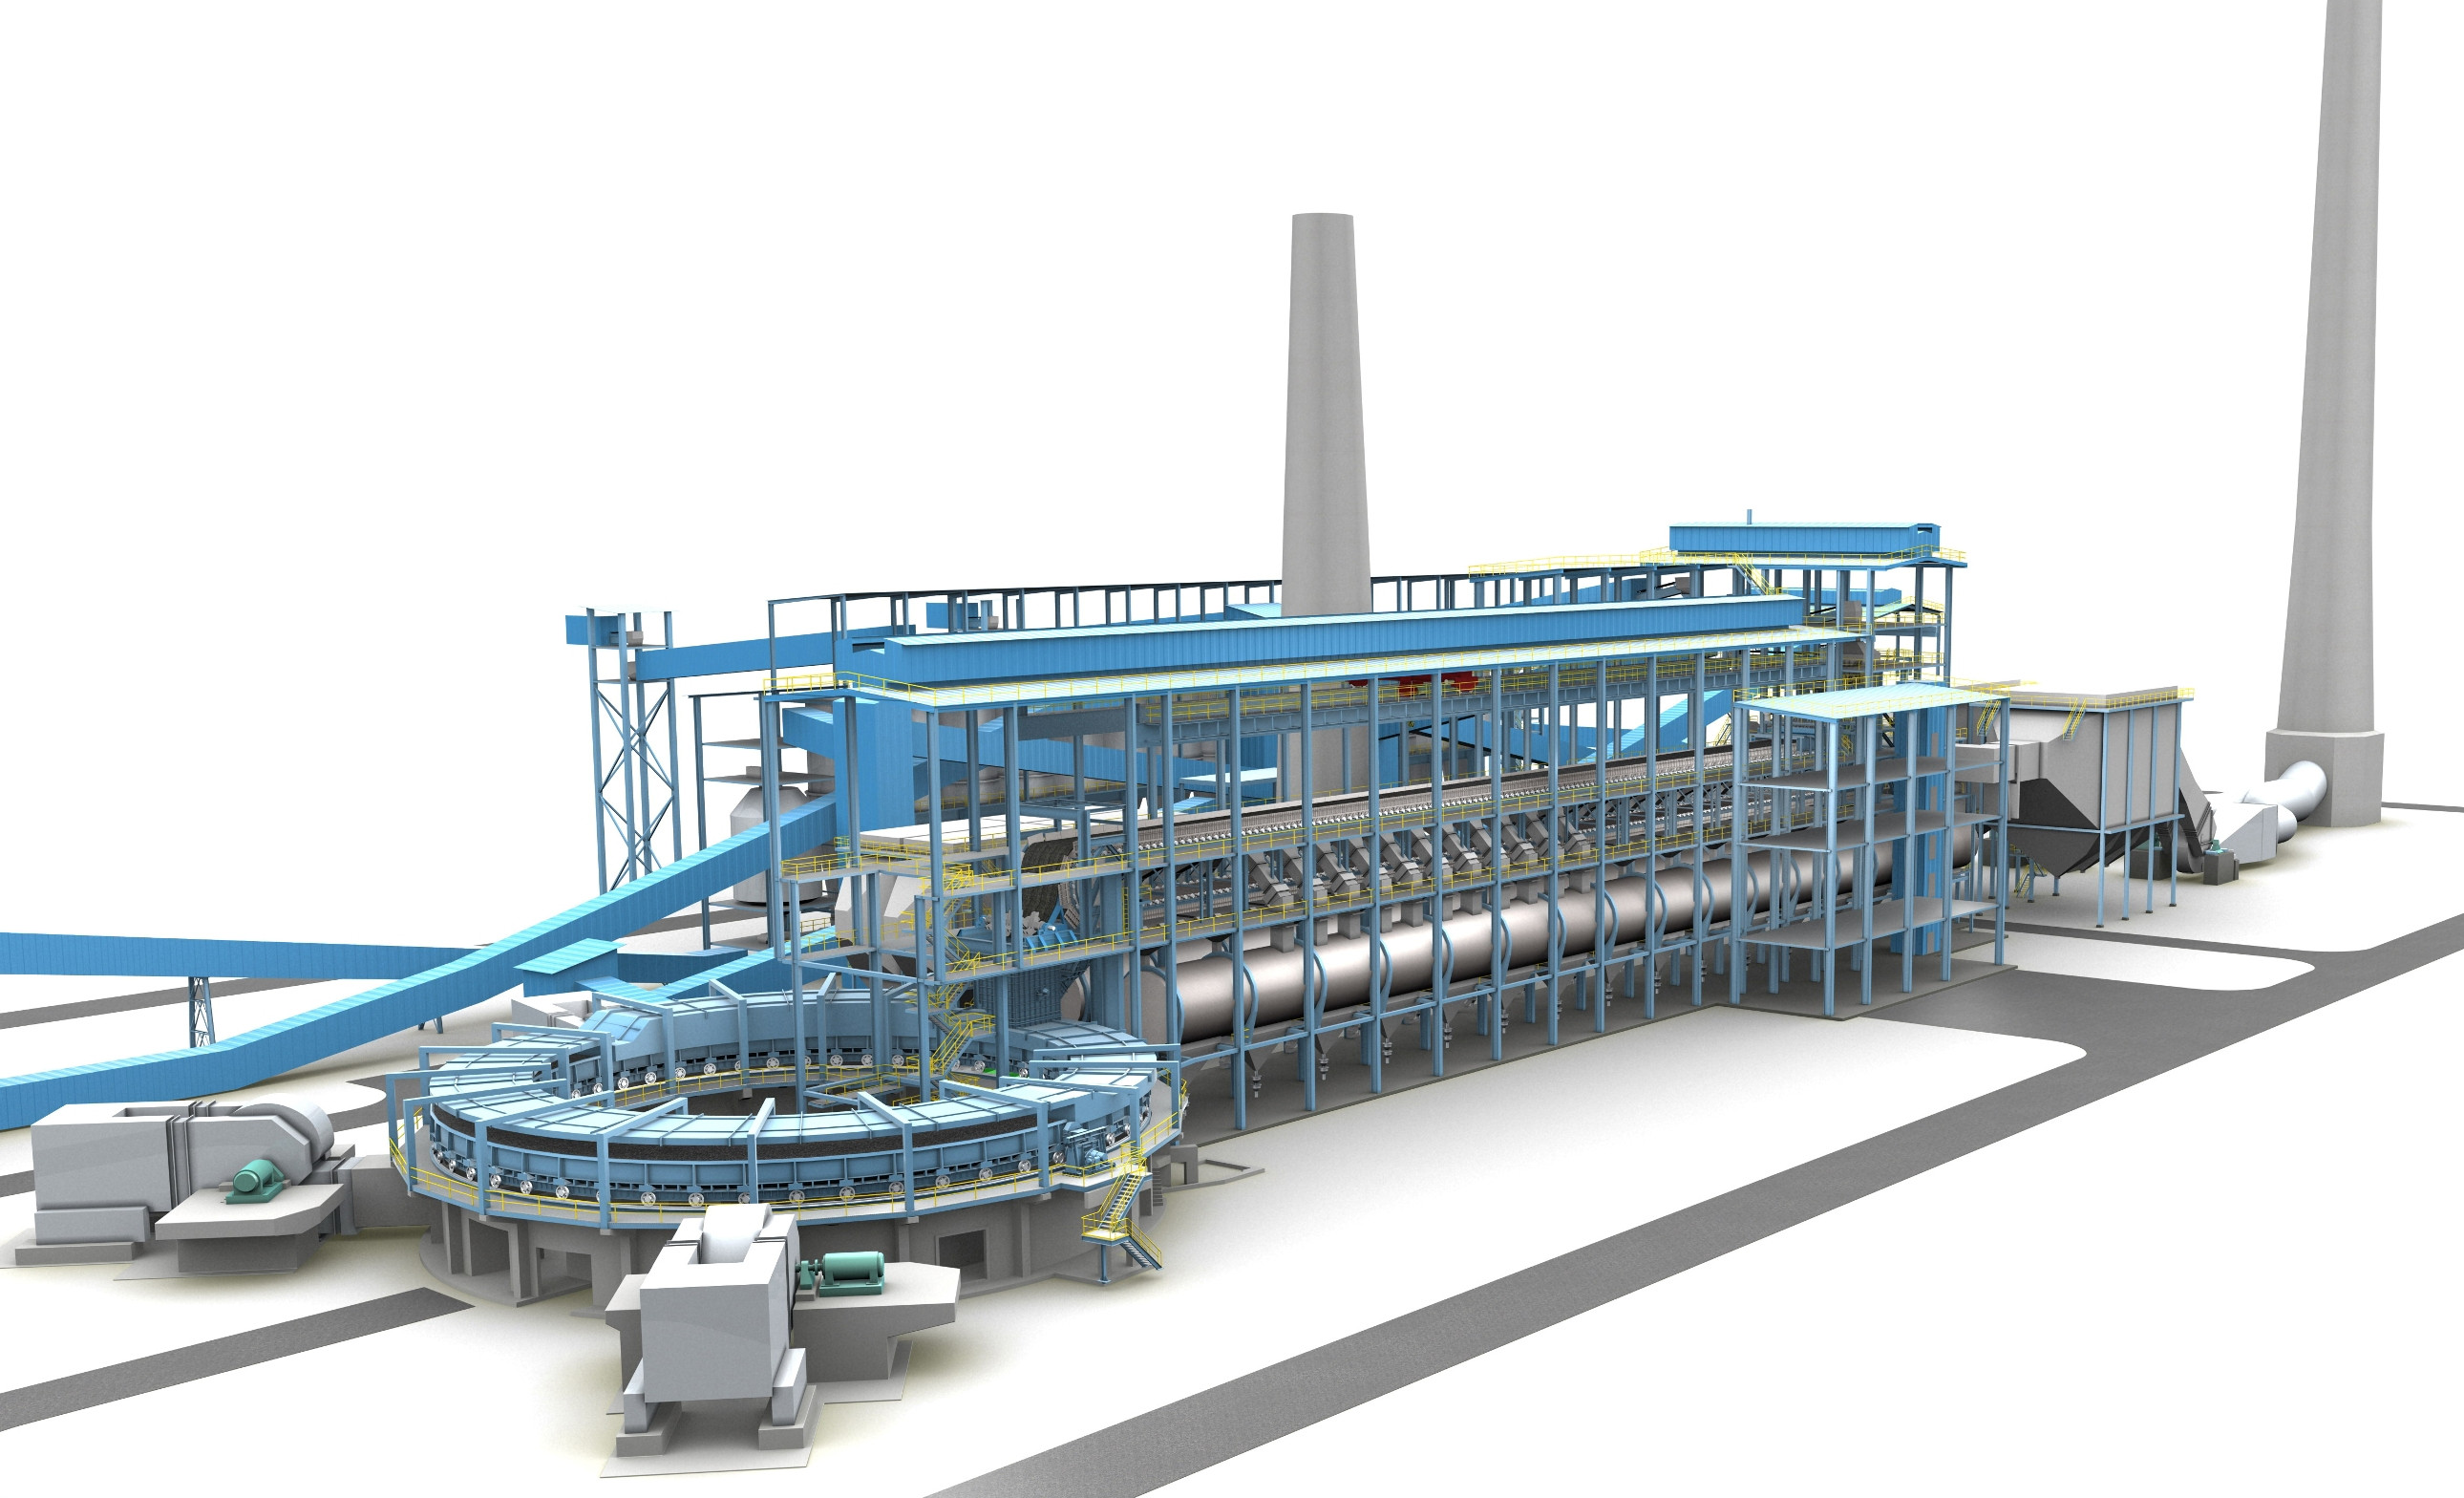
\includegraphics[width=.92\columnwidth]{images/124sinterplant}
\caption[Sinter plant]{Sinter plant (Primetals GmbH).}
\label{fig:124sinterplant}
\end{figure}
Instead, fines need to be sintered. 
Sintering consists in partially melting the
fines with limestone and coke.\\
The resulting granular material needs nonetheless to be cooled for
transportation and storage. 
The metallurgical industry uses a \textit{sinter chute cooling system} for this
purpose, see Fig. \ref{fig:124sinterplant}, with many phases:
\begin{enumerate}
  \item{Hot particles are fed into a chute, which deposits the
  particles on a rotating system and segregates them, i.e. lays the large
  particles on the bottom and the small ones on top.}
  \item{Air is injected from the bottom of the rotating system, cooling the
  particles.}
  \item{The resulting particles larger than 25 millimiters are crushed, and
  reinserted in the flow.}
  \item{The particles smaller than 7 millimiters are melted once
  more.}
  \item{The particles between 7 and 25 millimiters are ready for blast furnace
  smelting.}
\end{enumerate}

In our thesis, we focused on (1), and the particles involved in this process.\\
Further, we investigated the more complex blast furnace smelting, with focus on
the raceway area, which can be seen in Fig. \ref{fig:125blastfurnace}.

\begin{figure}[!htb]
\centering
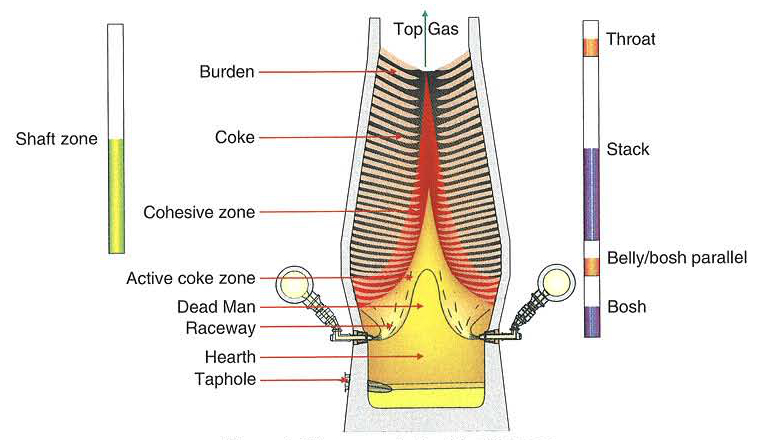
\includegraphics[width=.86\columnwidth]{images/125blastfurnace}
\caption[Blast furnace scheme]{Blast furnace scheme \cite{RefWorks:200}.}
\label{fig:125blastfurnace}
\end{figure}

\section{Materials characterization}
\label{sec:materialscharacterization}

A univocal
method to characterize these particles has so far not been established.
From the experimental point of view, the main issues are the difficult setups and the general 
reliability and reproducibility of the tests. 
From the numerical point of view, no general procedure is available, and the existence of a 
mathematically unique solution describing macro/micro particle contact has yet
to be proved.\\
Moreover, in a recent study, \citet{RefWorks:56} implied "that the dynamic properties of a 
powder cannot be applied to universally predict the static properties of a powder, and, likewise, 
the static properties cannot be used to predict dynamic properties".\\

\section{DEM Simulations}
\label{sec:demsimulations}

Many authors used \acs{DEM}, the discrete
element method used in this work, to understand sintering processes 
\cite{RefWorks:196, RefWorks:197} and smelting \cite{RefWorks:198,
RefWorks:199}.\\
In their original formulation of \acs{DEM} \citet{RefWorks:172} allowed two particles to slightly overlap upon
contact, see Fig. \ref{fig:062collision}, and consequently they proposed
repulsive forces in relation to this overlap distance.
\begin{figure}[!htb]
\centering
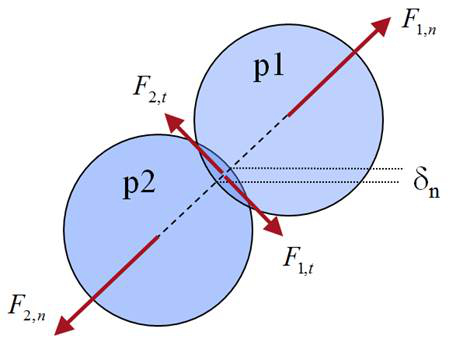
\includegraphics[width=.50\columnwidth]{images/062collision}
\caption[Soft sphere model]{Soft sphere model.}
\label{fig:062collision}
\end{figure}
The force that particle $i$ exerts on particle $j$ is defined as:
\begin{equation}
m \ddot{x}_{ij} + c \dot{x}_{ij} + k x_{ij} =  F_{ij} .
\label{equ:newtonlaw}
\end{equation}

Their fundamental modelling concept of \acs{DEM} has
since been widely accepted in the literature and their soft sphere contact law has been developed further by
numerous researchers (\citet{RefWorks:148} and \citet{RefWorks:145}).
With increasing computational resources, \acs{DEM} simulations have become very
popular giving rise to the development of commercial (e.g., $PFC3D$, used by
\citet{RefWorks:87}) and open-source software (e.g.,
\acs{LIGGGHTS}, \citet{RefWorks:136}, \citet{RefWorks:139}).
Soft-sphere \acs{DEM} simulations of thousands of particles have been proven to 
faithfully model particle bulk behaviour, as in Fig. \ref{fig:061cfdemsim}
(\citet{RefWorks:86}).\\
\begin{figure}[!htb]
\centering
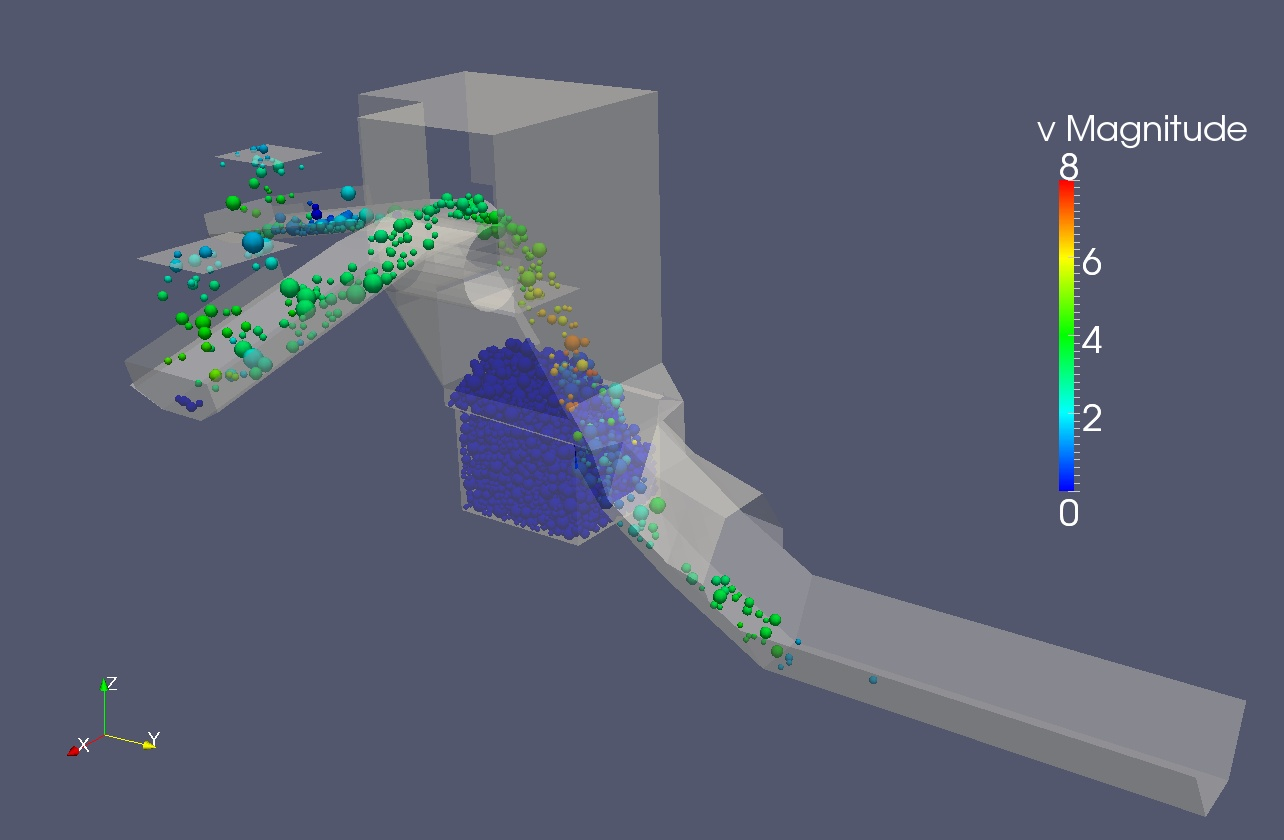
\includegraphics[width=.70\columnwidth]{images/061cfdemsim}
\caption[DEM simulation]{Example of a DEM simulation (www.cfdem.com).}
\label{fig:061cfdemsim}
\end{figure} 

\section{Parameters}
\label{sec:parameters}

In these macroscopic \acs{DEM} simulations, the contact law kernel between a 
pair of particles determines the global bulk behaviour of the granular material
(\citet{RefWorks:131}).
As a consequence, defining a correct contact law is of crucial importance for the predictive 
capability of \acs{DEM} simulations. 
Since \acs{DEM} contact laws are based 
on a set of semi-empirical parameters, correct contact law 
parameters must be defined for a given granular material
or \acs{DEM} simulations will fail (\citet{RefWorks:177}). \\
Identifying \acs{DEM} contact law parameters is not a trivial task. 
Due to the huge number of particles in a granular material, it
may be impractical to identify valid parameter sets by performing bilateral 
particle collision experiments. 
Furthermore, some contact law parameters such as the coefficient of rolling
friction are purely empirical and cannot be determined by direct 
particle-to-particle measurements (\citet{RefWorks:87}).
Therefore, \acs{DEM} contact law parameters (Table \ref{tab:08DEMparameters}) are
commonly determined by comparing the macroscopic outcome of large-scale \acs{DEM}
simulations with bulk experiments (\citet{RefWorks:91}). 
If \acs{DEM} simulation results disagree with bulk measurements, the set of contact
law parameters must be adjusted until reasonable agreement is achieved.\\
However, this purely forward methodology of parameter identification is limited by 
the multi-dimensionality of the parameter space and the associated computational costs of the required 
\acs{DEM} test simulations. 
Moreover, one parameter set which is valid for one bulk behaviour (e.g., angle
of repose) might fail for another (e.g., shear tester). \\

\subsection{Direct Determination}
\label{subsec:directdetermination}

\begin{figure}[!htb]
\centering
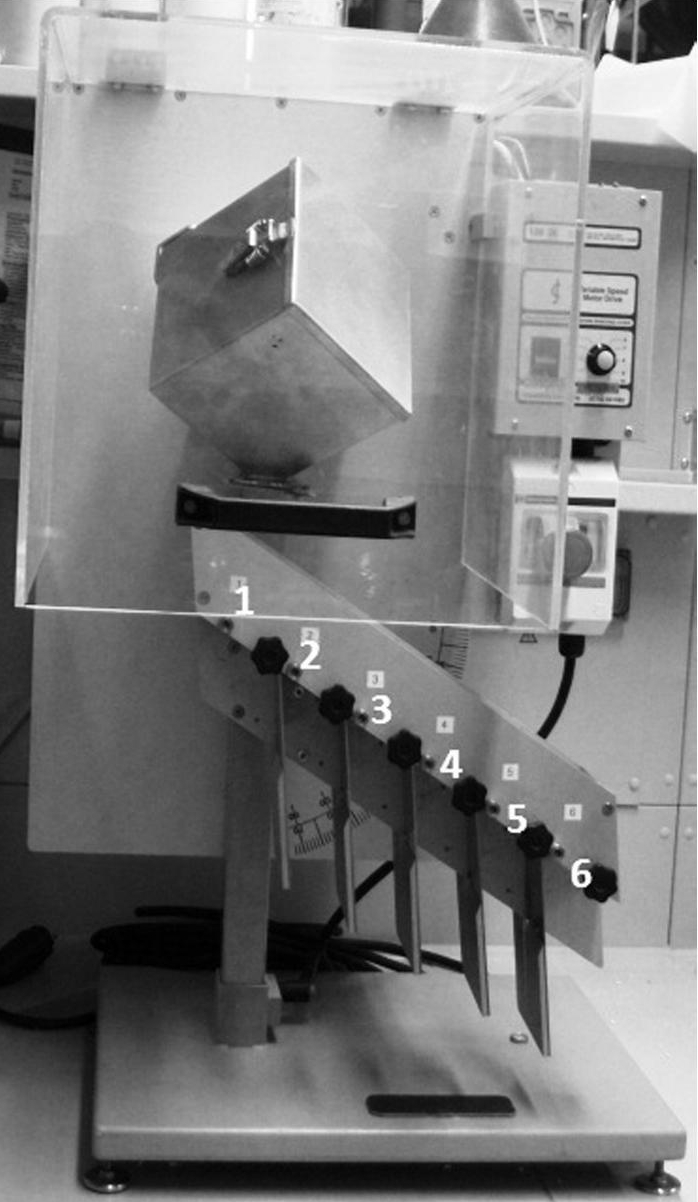
\includegraphics[width=.30\columnwidth]{images/126qpmtester}
\caption[QPM tester]{QPM tester \cite{RefWorks:177}.}
\label{fig:126qpmtester}
\end{figure}
There are yet ways to determine contact parameters directly by measuring
material properties or by performing particle based experiments, see e.g.
\citet{RefWorks:177}, \citet{RefWorks:181}, and \citet{RefWorks:186}, as in
Fig. \ref{fig:126qpmtester}.\\
However, these methodologies are laborious, 
since they have to be performed for every new granular material prior to a \acs{DEM}
simulations. 
Especially for the already cited rolling friction parameter, it is arduous to
link the rolling friction parameter to the non-sphericity of the particle. \\
Clearly, there is a
need for an efficient method for identifying \acs{DEM} contact law parameters, given
a specific particle behaviour.




% !TEX encoding = UTF-8
% !TEX TS-program = pdflatex
% !TEX root = ../Tesi.tex
% !TEX spellcheck = en-EN

%************************************************
\chapter{Aim of this Thesis}
\label{cap:aim}
%************************************************

In our study, we harnessed Artificial Neural Networks (\acs{ANNs}) in order to
reduce the number of \acs{DEM} test simulations required
to characterize bulk materials for large scale simulations. \\
As the following chapters will show, we divided this task in two sections:
\begin{enumerate}
  \item{identification of \acs{DEM} parameters, in part
  \ref{par:identification},}
  \item{applications, in part \ref{par:applications}.}
\end{enumerate}

\section{Aim for Neural Network}
\label{sec:aimforneuralnetwork}

\acs{ANNs} have proven to be a versatile tool in analysing complex, non-linear
systems of multi-dimensional input streams (Vaferi et al. \cite{RefWorks:150}, Witten et
al. \cite{RefWorks:174} and Haykin \cite{RefWorks:158}).
In our case, we fed an \acs{ANN} with \acs{DEM} contact law parameters as input
and compared the output with the bulk behaviour 
predicted by a corresponding \acs{DEM} simulation. 
The difference between \acs{ANN} prediction and \acs{DEM} prediction was used to
train our specific \acs{ANN} with a backward-propagation algorithm. 
\begin{figure}[!htb]
\centering
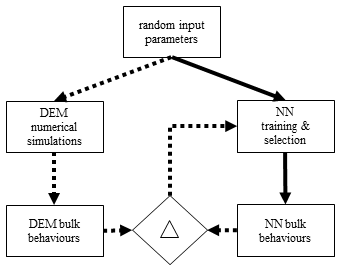
\includegraphics[width=.50\columnwidth]{images/127anntraining}
\caption[ANN training]{ANN training.}
\label{fig:127anntraining}
\end{figure}
After a training phase comprising a limited number of \acs{DEM} test simulations,
the \acs{ANN} could then be used as a stand-alone prediction tool for the bulk behaviour of a 
granular material in relation to \acs{DEM} contact law parameters, see Fig.
\ref{fig:127anntraining}. \\
In this study, we applied this parameter identification method to two different
granular bulk behaviours, namely the angle of repose (\acs{AoR}) test and the
Schulze shear cell (\acs{SCT}) test.
In both cases, we first trained a specific \acs{ANN} using a number of \acs{DEM} test
simulations before we identified valid sets of \acs{DEM} contact law parameters by
comparing the stand-alone \acs{ANN} predictions with corresponding bulk experiments. 
For both cases we obtained valid sets of contact law parameters, 
which we then compared to formulate a reliable contact law for a given
granular material.
We further showed that the same \acs{ANN} could be used to characterize different
granular materials, which have the same particle behaviour and could modelled with the same contact
law.
% !TEX encoding = UTF-8
% !TEX TS-program = pdflatex
% !TEX root = ../Tesi.tex
% !TEX spellcheck = en-EN

%************************************************
\part{Theory}
\label{par:theory}
%************************************************

%\improvement{Write something?}
% !TEX encoding = UTF-8
% !TEX TS-program = pdflatex
% !TEX root = ../Tesi.tex
% !TEX spellcheck = en-EN

%************************************************
\chapter{Discrete Element Method}
\label{cap:dem}
%************************************************


\begin{itemize}
  \item{Molecular Dynamics;}
  \item{Discrete Element Method:
  \begin{itemize}
  \item{Hard spheres approach;}
  \item{Soft spheres approach.}
\end{itemize} }
\end{itemize}

%\section{DEM}
%\label{sec:dem}
For each particle i inside the domain, a Discrete Element Method ($DEM$) code
follows the trajectory and calculates the force that particle i exerts on particle j.
The main forces involved are: gravity, contact forces due to collisions, and
further interactions such as electrostatic, Van der Waals, cohesive forces and fluid-solid interactions in 
multiphase flows. 

\section{Hard spheres approach}
\label{sec:hardspheresapproach}
\info{words on hard spheres approach}

\section{Soft spheres approach}
\label{sec:softspheresapproach}

Contact models:
\begin{itemize}
  \item{Hooke;}
  \item{Hertz.}
\end{itemize}
Rolling friction:
\begin{itemize}
  \item{cdt;}
  \item{epsd;}
  \item{epsd2.}
\end{itemize}

\subsection{Hooke}
\label{subsec:hooke}

\subsection{Hertz}
\label{subsec:hertz}

For the raw material used in this work 
Di Renzo and Di Maio \cite{RefWorks:145} suggested using the non-linear
Hertzian model without cohesion for the particle-particle and particle-wall contacts. 
This granular model uses the following formula for the contact force between two granular particles (Eq. \ref{eq:forceij}):
%************************************************
\begin{equation}
 F_{ij} = 
\begin{cases}
F_{n,ij} + F_{t,ij} = \left( k_n \delta_{n,ij} + \gamma_n v_{n,ij} \right) + \left( k_t \delta_{t,ij} + \gamma_t v_{t,ij} \right) & \text{if } r < d ,\\
0    & \text{if } r > d ,\\
\end{cases}
 \label{eq:forceij}
\end{equation}

%************************************************
where the subscript $n$ stands for normal and $t$ for tangential. 
Here, $k$ and $\gamma$ are respectively the stiffness and damping coefficients, 
while $\delta$ and $v$ are the displacement and the velocity, $r$ is the
distance between two particles of radii $R_i$ and $R_j$, and $d = R_i + R_j $ is
the contact distance.
Both the normal and the tangential
force comprise two terms, a spring force and a damping force. 
The tangential (or shear) force is a ``history'' effect that accounts for the
tangential displacement (``tangential overlap'') between the particles for the
duration of contact.
The $k_n$, $k_t$, $\gamma_n$, and $\gamma_t$ coefficients are calculated from
the material properties as follows:
%************************************************
\begin{equation}
\begin{aligned}
	k_n &= \frac{4}{3} E_{eq} \sqrt{R_{eq} \xi_n} ,\\
	\gamma_n &= 2 \sqrt{\frac{5}{6}} \beta \sqrt{S_n m_{eq}} ,\\
	k_t &= 8 G_{eq} \sqrt{R_{eq}} \xi_n ,\\
	\gamma_t &= 2 \sqrt{\frac{5}{6}} \beta \sqrt{S_t m_{eq}} .
\end{aligned}
\label{eq:hertz}
\end{equation}

%************************************************
In addition to the equations \ref{eq:hertz} the following relations (Eqns. \ref{eq:equivProp2}) are required:
%************************************************
\begin{equation}
\begin{aligned}
 \frac{1}{E_{eq}} & = \frac{1-\nu_i^2}{E_i} + \frac{1-\nu_j^2}{E_j} ,\\
 \frac{1}{G_{eq}} & = \frac{2(2+\nu_i)(1-\nu_i)}{E_i} + \frac{2(2+\nu_j)(1-\nu_j)}{E_j} ,\\
 \frac{1}{R_{eq}} &= \frac{1}{R_i} + \frac{1}{R_j} ,\\
 \frac{1}{m_{eq}} &= \frac{1}{m_i} + \frac{1}{m_j} ,\\
 \beta & = \frac{\ln(e)}{\sqrt{ln^2(e)+\pi^2}} ,\\
 S_n & = 2 E_{eq} \sqrt{R_{eq} \delta_n} ,\\
 S_t & = 8 G_{eq} \sqrt{R_{eq} \delta_n} ,\\
 k_r & = k_t R_{eq}^2 .\\
\end{aligned}
\label{eq:equivProp2}
\end{equation}


%************************************************

In the paper by Wensrich and Katterfeld \cite{RefWorks:87}, further details on
the method can be found.\\
In the contact law we used, 
the tangential component of the contact force between two generic particles
($F_t$) is truncated to fulfil:
%************************************************
\begin{equation}
F_{t,ij} \leq \mu_s F_{n,ij},
 \label{eq:force_t}
\end{equation}

%************************************************

where $F_n$ is the normal component and $\mu_s$ is the coefficient of sliding
friction, one of the particle-based $DEM$ parameter we investigated, 
another being the coefficient of rolling friction ($\mu_r$). 

\subsection{EPSD2}
\label{subsec:epsd2}

For coarse non-spherical particles, this is a critical parameter and describes
inter-particle friction in medium to dense granular flow simulations. It is proportional to the 
torque counteracting the rotation of the particle. The $\mu_r$ parameter enters the 
equations according to the elasto-rolling resistance model presented by Wensrich and 
Katterfeld \cite{RefWorks:87} and Ai et al. \cite{RefWorks:131} 
based on the work of Jiang et al. \cite{RefWorks:143}. 
The model is called $EPSD2$ in $LIGGGHTS$ and is appropriate for both one-way and cyclical rolling cases.
The maximum magnitude of rolling resistance torque is (Eq. \ref{eq:trmax}):

%************************************************
\begin{equation}
T_{r~max} = \mu_r R_r |\tilde{F_n}| ~,
 \label{eq:trmax}
\end{equation}

%************************************************

where $R_r$ is the equivalent radius and $F_n$ the normal force.
The last two particle-based $DEM$ parameters we investigated were $\rho_p$
and the coefficient of restitution ($COR$) as defined by Ai. et al.
\cite{RefWorks:131}.\\

\improvement{ADD ACRONYM table AND CSV LIST HERE}

\ref{tab:08DEMparameters}\\
\ref{tab:14bulkvalues}\\
\begin{table}[h]
\centering
\begin{tabular}{l}
\hline 
    Radius \ac{R} (m)   \\ [5pt]

	Size distribution (-) \\ [5pt]

    Young's modulus \ac{E} (Pa)  \\ [5pt]

    Poisson's ratio \ac{nu} (-) \\ 
     Time step \ac{deltat} (s) \\ [5pt]
        \hline
     Coefficient of sliding friction \ac{mus} (-)\\  [5pt]
    Coefficient of rolling friction \ac{mur} (-) \\ [5pt]
    Coefficient of restitution \ac{CoR} (-)   \\ [5pt]
     Particle density $\ac{rhop} = \frac{mass ~ of ~ one ~ particle}{volume ~ of
     ~ one ~ particle}$ ($kg/m^3$)  \\ [5pt]
     Geometry factor \ac{dCylDp} (-)  \\ [5pt]
   
\hline
\end{tabular}
\caption[DEM parameters]{DEM parameters. The upper parameters were
identical in all simulations. The lower parameters were constant in each
simulation, but were varied between simulations.}
\label{tab:08DEMparameters}
\end{table}


\begin{table}[h]
  \centering
    \begin{tabular}{lcc}
    \hline
     & acronym & formula \\ 
     \hline
    bulk density & \ac{rhob} & $\frac{mass ~ of ~ the ~ bulk}{volume ~ of ~ the ~ bulk}$ \\ 
    [5pt]
     
    steady-state flow/pre-shear coefficient of internal friction & \ac{mupsh}
     & $\frac{\tau_{psh}}{\sigma_{n,psh}}$ \\      [5pt]
     
    incipient flow/shear coefficient of internal friction & \ac{mush} &
    $\frac{\tau_{sh}}{\sigma_{n,sh}}$ \\      [5pt]
     
    static angle of repose & \ac{AoR}   & from the slope \\
\hline
    
    \end{tabular}%
  \caption{Values representative of bulk behaviour.}
\label{tab:14bulkvalues}
\end{table}%

\section{Literature Values}
\label{sec:literaturevalues}

\improvement{Discuss about literature values for all parameters (ref.
Combarros, Paulick).}
%% !TEX encoding = UTF-8
% !TEX TS-program = pdflatex
% !TEX root = ../Tesi.tex
% !TEX spellcheck = it-IT

%************************************************
\chapter{Computational Fluid Dynamics}
\label{cap:cfd}
%************************************************

\lipsum[1]


% !TEX encoding = UTF-8
% !TEX TS-program = pdflatex
% !TEX root = ../Tesi.tex
% !TEX spellcheck = en-EN

%************************************************
\chapter{Artificial Neural Network}
\label{cap:ann}
%************************************************

\section{Probability theory}
\label{sec:probability}

\citet{RefWorks:194} defines $X$ a random variable with a fixed domain $Val(X)$,
showing aspects of the system's world. In this world, a fixed assignment of
values to variables (from one to all) is called an $event$.
Given a probability distribution $P$, this assigns to the specific event
$\alpha$ a value: $P(\alpha)$.
Provided a random variable $X$, whose $Val(X) = \{ x^1, \ldots , x^k \}$, a
\textit{Probability Distribution} over $X$ is $P(X) = \{ P(x^1), \ldots , P(x^k)
\}$.
He further defines, given a second random variable $Y$:
\begin{itemize}
  \item {Probability of conjunction of events, $P(X = x, Y = y)$ or $P(x, y)$,
  or $P((X = x) \cap (Y = y))$;}
  \item {A set of variables, $\mathbf{X} = \{X_1, X_2, \ldots , X_k \}$;}
  \item {Joint distribution over one set of variables, $P(\mathbf{X}) =
  P(X_1, X_2, \ldots , X_k) $;}
  \item {Joint distribution over two sets of variables, $P(\mathbf{X, Y}) =
  P(X_1, X_2, \ldots , X_k, Y_1, Y_2, \ldots , Y_l  ) $;}
  \item {Conditional distribution, $P(\mathbf{X | Y}) =
  P(X_1, X_2, \ldots , X_k | Y_1, Y_2, \ldots , Y_l  ) $.}
\end{itemize}

For later reference, we write two fundamental rules of the probability theory,
the sum rule (Eq. \ref{eq:sumrule}) and the product rule (Eq.
\ref{eq:productrule}), from which Bayes derived his theorem (Eq.
\ref{eq:bayestheorem}):
\begin{equation}
\label{eq:sumrule}
P(X) = \sum_Y {P(X, Y)}, 
\end{equation}

\begin{equation}
\label{eq:productrule}
P(X, Y) = P(Y | X) \cdot P(X), 
\end{equation}

\begin{equation}
\label{eq:bayestheorem}
P(Y | X) = \frac{P(X | Y) \cdot P(Y)}{P(X)}.
\end{equation}


\subsection{The Gaussian Distribution}
\label{subsec:gaussian}

Provided a single real valued variable $x$, a Gaussian distribution is:
\begin{equation}
\label{eq:gaussiandistribution}
\mathcal{N}(x | \mu, \sigma^2) = \frac{1}{(2 \pi \sigma^2)^{0.5}} exp \left\{
 - \frac{1}{2 \sigma^2} (x - \mu)^2	\right\} ,
\end{equation}

where $\mu$ is the mean and $\sigma^2$ is the variance, of which the square root
is the standard deviation.
Further, $\beta = 1/\sigma^2$ is the deviation.
Given a set of observations $\mathbf{x} = (x_1, \ldots, x_N)^T$, assumed
\textit{indipendent and identically distributed} (i.i.d.), the probability of
the data set becomes:
\begin{equation}
\label{eq:likelihoodgaussian}
p(\mathbf{x} | \mu, \sigma^2) = \prod_{n = 1}^{N} \mathcal{N}(x | \mu,
\sigma^2),
\end{equation}
which can be more easily computed if written in a logaritmic form:
\begin{equation}
\label{eq:loglikelihoodgaussian}
ln p(\mathbf{x} | \mu, \sigma^2) = - \frac{1}{2 \sigma^2} \sum_{n = 1}^{N}{(x_n
- \mu)^2} - \frac{N}{2} ln (\sigma^2) - \frac{N}{2} ln (2 \pi) .
\end{equation}
To obtain the expectation of this likelihood Equation
\ref{eq:loglikelihoodgaussian} can be maximized over $\mu$ and $\sigma^2$,
giving respectively Eq. \ref{eq:mu} and Eq. \ref{eq:sigma}:
\begin{equation}
\label{eq:mu}
\mathbb{E}[\mu_{ML}] = \mathbb{E}\left[\frac{1}{N} \sum_{n =
1}^{N}{(x_n)}\right] = \mu ,
\end{equation}
\begin{equation}
\label{eq:sigma}
\mathbb{E}[\sigma^2_{ML}] = \mathbb{E}\left[\frac{1}{N} \sum_{n = 1}^{N}{(x_n -
\mu_{ML})^2} \right] = \left( \frac{N - 1}{N} \right) \sigma^2.
\end{equation}
In case of a D-dimensional vector $\mathbf{x}$, we write the multivariate
Gaussian distribution as:
\begin{equation}
\label{eq:multivariategaussiandistribution}
\mathcal{N}(\mathbf{x} | \boldsymbol{\mu}, \mathbf{\Sigma}) = 
\frac{1}{(2 \pi)^{D/2} |\boldsymbol\Sigma|^{0.5}} 
exp \left\{ - \frac{1}{2} (\mathbf{x} - \boldsymbol{\mu})^T 
\boldsymbol\Sigma^{-1}  (\mathbf{x} - \boldsymbol{\mu})
\right\} ,
\end{equation}

where $\mathbf{\Sigma}$ is the covariance matrix.


\section{Regression statistics}
\label{sec:regressionstatistics}

Statistics finds relationship between random variables.
Once one of them ($response$) is chosen, it infers its dependance from the
others ($regressors$), also including an additive $error$ term
(\citet{RefWorks:194}). We call this a \textit{regression model}, which can be
linear or nonlinear.
In this work we exploited the following regression models:
\begin{itemize}
  \item{Bayesian linear,}
  \item{Gaussian non linear,}
  \item{Artificial Neural Network (\acs{ANN}).}
\end{itemize}
We later explained, section \ref{sec:annmodeldev}, why we focused on the last
one over the other two.
% The B and the  regressions 
% can be used as regression methods for \acs{DEM} identification
% and as benchmark for more precise tools. 
%to further
%assess the quality of the \acs{ANNs} training.

\subsection{Supervised learning}
\label{subsec:supervisedlearning}

The learning processes available for a regression model are:

\begin{itemize}
  \item{supervised learning, or learning with a teacher,}
  \item{semi-supervised learning,}
  \item{unsupervised learning.}
\end{itemize}

The easiest regression model consists in fitting target data
points (exptected response) with a polynomial curve.
The cofficients of the curve are obtained by minimizing a cost function, which
is proportional to the distance of said data points to the curve.
The expected response represents the teacher of the system.
The network is trained in \textit{batch mode}, all the examples are known before
starting the training.
Further, these examples were assumed to be \textit{independent and identically
distributed}.
We focused on supervised learning: the materials we investigated
are examined in batch, not online.\\
\citet{RefWorks:194} defines \textit{supervised learning} an application, where all the
training examples comprises the input vectors and their corresponding target
vectors.
%\subsection{Gaussian non linear regression}
%\label{subsec:gaussiannonlinearregression}
% \improvement{I focus only on supervised learning, but also unsupervised
% learning and semi-supervised learning exist.}


\subsection{The Standard Bayesian Linear Model}
\label{subsec:standardlinearmodel}

\citet{RefWorks:192} define the standard linear regression model with Gaussian noise as:
\begin{equation}
\label{eq:standardlinearregression}
y = \mathbf{x}^T \mathbf{w} + \varepsilon,
\end{equation}

where $\mathbf{x}$ is the input vector, $\mathbf{w}$ are the weights of the
linear model, and $y$ is the target value. The noise $\varepsilon$ adopts an
$i.i.d.$ Gaussian distribution:
\begin{equation}
\label{eq:noise}
\varepsilon = \mathcal{N}(0, \sigma_n^2).
\end{equation}

Extending to the n-dimensional case, we have a set of $n$ observations:
\begin{equation}
\label{eq:observations.tex}
\mathcal{D} = \{ (\mathbf{x}_i, y_i) | i = 1, \ldots, n \} = (X, \mathbf{y}).
\end{equation}

Consequently, the $likelihood$, or probability density of the observations given
the parameters, becomes:
\begin{equation}
\label{eq:likelihoodcontinuous}
\begin{align*}
p(\mathbf{y} | X, \mathbf{w}) &= \prod_{i = 1}^{n} {p(y_i | \mathbf{x}_i,
\mathbf{w})} = \prod_{i = 1}^{n} {\frac{1}{\sqrt{2\pi} \sigma_n} 
exp \left(- \frac{(y_i - \mathbf{x}_i^T \mathbf{w})^2}{2 \sigma_n^2} \right)} \\
&= \frac{1}{(2\pi \sigma_n^2)^{n/2}} exp \left(- \frac{1}{2 \sigma_n^2}
|\mathbf{y} - X^T \mathbf{w}|^2 \right) = \mathcal{N}(X^T \mathbf{w}, \sigma_n^2
I), 
\end{align*}
\end{equation}
where the Euclidean length of vector $\mathbf{v}$ is indicated by
$|\mathbf{v}|$.
We also consider the weights $\mathbf{w}$ proportional to the Gaussian
distribution with zero mean and variance equal to the coviarance matrix
$\Sigma_p$.\\
Remembering the theorem of Bayes, Eq. \ref{eq:bayestheorem}, which states that:
\begin{equation}
\label{eq:bayestheoremword}
posterior = \frac{likelihood \times prior}{marginal ~ likelihood},
\end{equation}

we can define the continuous posterior distribution as:
\begin{equation}
\label{eq:bayestheoremcontinuous}
p(\mathbf{w | y }, X) = \frac{p(\mathbf{y} | X, \mathbf{w}) \cdot
p(\mathbf{w})}{p(\mathbf{y} | X)},
\end{equation}

where the \textit{marginal likelihood} is:
\begin{equation}
\label{eq:marginallikelihood}
p(\mathbf{y} | X) = \int{p(\mathbf{y} | X, \mathbf{w} p(\mathbf{w}) d
\mathbf{w}}.
\end{equation}

A first estimation of the posterior can be determined as follow:
\begin{equation}
\label{eq:likelihoodprior}
\begin{align*}
p(\mathbf{w} | X, \mathbf{y}) 
& \propto exp(- \frac{1}{2 \sigma_n^2} (\mathbf{y} - X^T \mathbf{w})^T
(\mathbf{y} - X^T \mathbf{w})) exp(- \frac{1}{2} \mathbf{w}^T \Sigma_p^{-1}
\mathbf{w}) \\
& \propto exp(- \frac{1}{2} (\mathbf{w} - \mathbf{\bar{w}})^T (\frac{1}{
\sigma_n^2} X X^T + \Sigma_p^{-1}) (\mathbf{w} - \mathbf{\bar{w}}))  \\
& \sim \mathcal{N}( \mathbf{\bar{w}} = \frac{1}{\sigma_n^2} A^{-1} X
\mathbf{y}, A^{-1}) ,
\end{align*}
\end{equation}

where $A = \sigma_n^{-2} X X^T + \Sigma_p^{-1}$.\\
An effective tool for the posterior predictive density of a variational Bayesian
multiple linear regression model is provided by \citet{RefWorks:193}.
% % \subsection{Bayesian linear regression}
% \label{subsec:bayesianlinearregression}

% We chose the Bayesian inference amongst the possible linear regression models.
%     a_0: shape parameter of the prior precision of coefficients
%     b_0: rate  parameter of the prior precision of coefficients
%     c_0: shape parameter of the prior noise precision
%     d_0: rate  parameter of the prior noise precision

% The theory is briefly explained in subsection \ref{subsec:bayesian linear
% regression}.
% \wrong{understand if the software requires as priors only the standard
% deviation or also the initial weights.}
% \info{to be continued}

\subsection{Gaussian Process}
\label{subsec:gaussianprocess}

\citet{RefWorks:192} define a \textit{Gaussian process} as a set of random variables. 
Any finite random of these variables have a joint Gaussian distribution.
The process $f(\mathbf{x})$ can be defined by its mean function $m(\mathbf{x})$
and its covariance function $k(\mathbf{x, x'})$, which are, respectively:
\begin{equation}
\label{eq:meanfunction}
m(\mathbf{x}) = \mathbb{E}\left[f(\mathbf{x}) \right],
\end{equation}
\begin{equation}
\label{eq:covariancefunction}
k(\mathbf{x, x'}) = \mathbb{E}\left[(f(\mathbf{x}) - m(\mathbf{x}))
(f(\mathbf{x'}) - m(\mathbf{x'})) \right],
\end{equation}
and it can be written in a compact form as:
\begin{equation}
\label{eq:gaussianprocess}
f(\mathbf{x}) \sim \mathcal{GP}(m(\mathbf{x}), k(\mathbf{x, x'})).
\end{equation}
In fact, the Bayesian linear regression model is a subcase of the Gaussian
process model, with the following conditions:
\begin{equation}
\label{eq:bayesianlinearmodelgaussianprocess}
\begin{align*}
f(\mathbf{x}) &= \boldsymbol{\phi(\mathbf{x})}^T \mathbf{w}, \\
\mathbf{w}	  & \sim \mathcal{N} (\mathbf{0}, \Sigma_p), \\
\mathbb{E}[f(\mathbf{x}) ] &= \boldsymbol{\phi(\mathbf{x})}^T
\mathbb{E}[\mathbf{w}] = 0, \\
\mathbb{E}[f(\mathbf{x}) f(\mathbf{x'})] &= \boldsymbol{\phi(\mathbf{x})}^T
\mathbb{E}[\mathbf{ww}^T] \boldsymbol{\phi(\mathbf{x'})} =
\boldsymbol{\phi(\mathbf{x})}^T \Sigma_p \boldsymbol{\phi(\mathbf{x'})}.
\end{align*}
\end{equation}
We used the \textit{squared exponential} (SE), also called Radial Basis Function
(RBF) or Gaussian Function, as covariance function. It defines the covariance
between a pair of random variables as:
\begin{equation}
\label{eq:covariancefunctionse}
cov(f(\mathbf{x}_p), f(\mathbf{x}_q)) = k(\mathbf{x}_p, \mathbf{x}_q) =
exp \left(-\frac{1}{2} |\mathbf{x}_p - \mathbf{x}_q|^2 \right) .
\end{equation}

Specifically, we handled the software developed by \citet{RefWorks:192} 
for Gaussian processes inference and prediction, although we constrained ourselves to the case of exact inference
(regression with Gaussian likelihood).
The complete description of the Gaussian non linear regression can be found in
\citet{RefWorks:194}.

\info{decide if using the equations from 5.3 to 5.7 of Rasmussen}

\section{Introduction on Artificial Neural Networks}
\label{sec:annintro}
%\improvement{Add some more details from Haykin introduction}
An Artificial Neural Network (\acs{ANN}) is a powerful regression model, 
based on non-linear functions (\citet{RefWorks:158}). 
In fact, we can see a neural network as a huge and parallel computer, composed
of many processing units. 
It stores experienced knowledge and translates it in
an usable form. 
The biological inspiration for artificial neural networks can be seen in Fig.
\ref{fig:049neuron1}. 
It resembles the human brain especially because it
uses a learning process to acquire knowledge, which is stored through the
synaptic weights.

\begin{figure}[!htb]
\centering
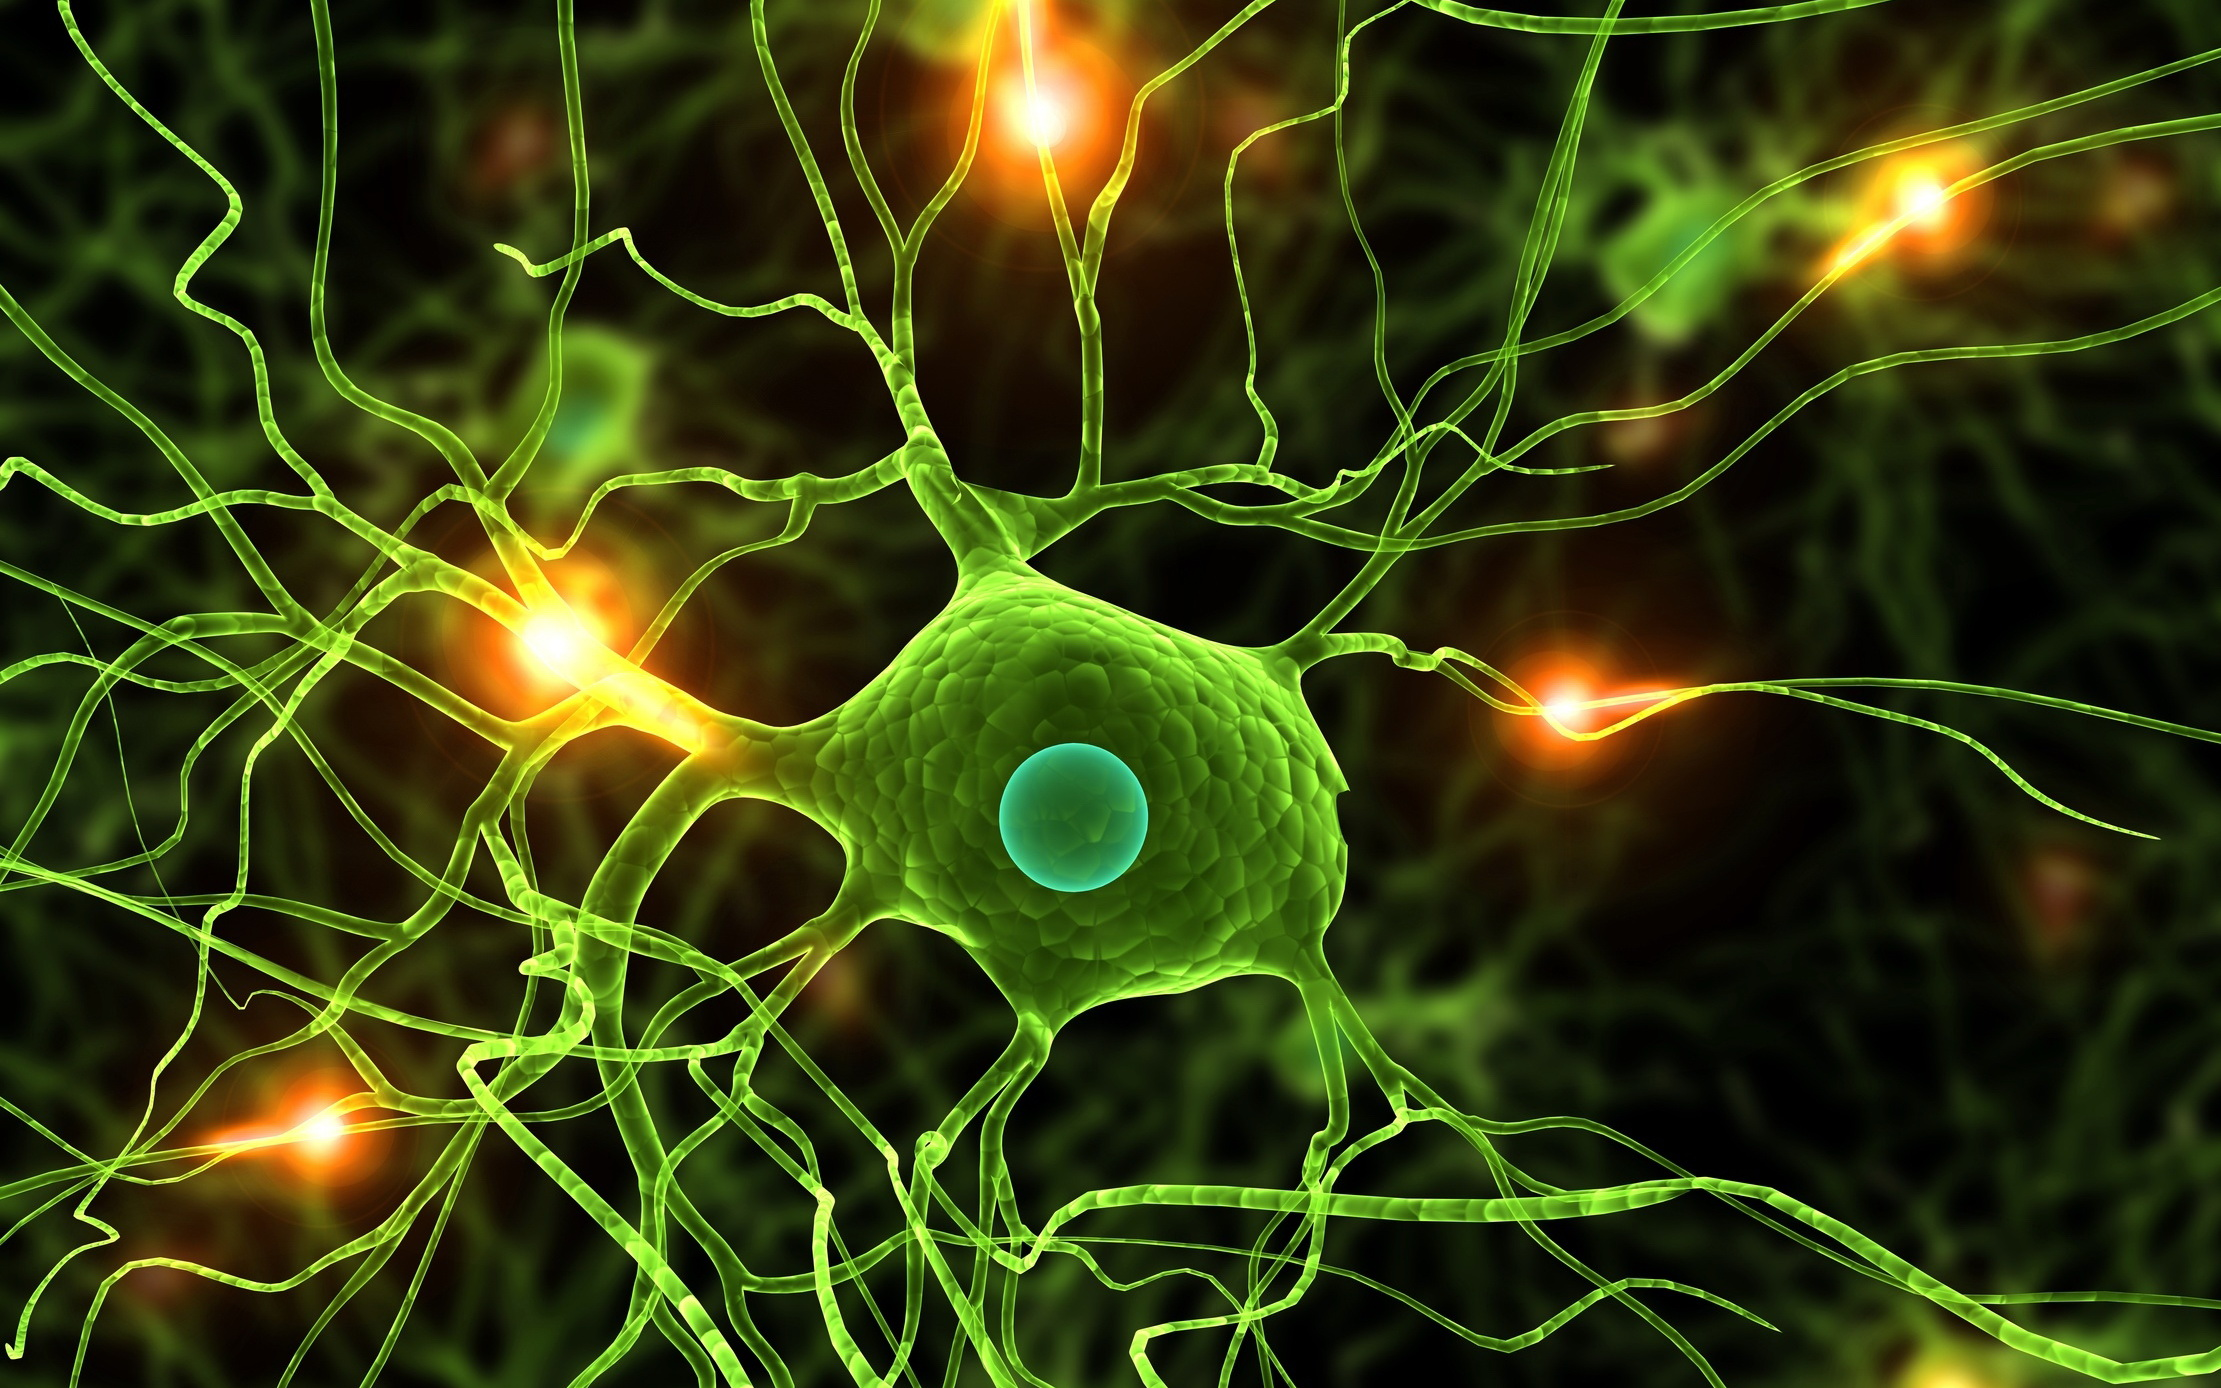
\includegraphics[width=.80\columnwidth]{images/049neuron1}
\caption[Biological inspiration 2]{Biological inspiration 2.}
\label{fig:049neuron1}
\end{figure}

In this work, we first used the \acs{ANN} to fit the \acs{DEM} numerical simulation
data, and then to process a vast number of parameters combinations. 
\acs{ANNs} map combinations of input data to convenient outputs (fitting). 
Amongst the available \acs{ANNs} were important for our context: 
\begin{itemize}
  \item {the Feedforward (\acs{FF}) \acs{ANN},}
  \item {the Radial basis function (\acs{RBF}) \acs{ANN}.}	
\end{itemize}
We did not investigate the latter.
For \acs{FF}-\acs{ANN},
numerous training algorithms are available. 
The most common are based on
backpropagation, e.g., Levenberg-Marquardt, Bayesian regulation and the scaled
conjugate gradient.

\section{Perceptron}
\label{sec:perceptron}

The basic element of an artificial neural network is the perceptron, a single
neuron, see Fig.
\ref{fig:064perceptron}, which is mathematically described by equation
\ref{eq:perceptron}: 
\begin{equation}
y = \varphi(b + \sum_{j = 1}^{m}{w_j \cdot x_j}),
 \label{eq:perceptron}
\end{equation}

where $x_j$ are the input nodes, $y$ is the output node, $w_j$ are the weights
and $b$ is the bias.
\begin{figure}[!htb]
\centering
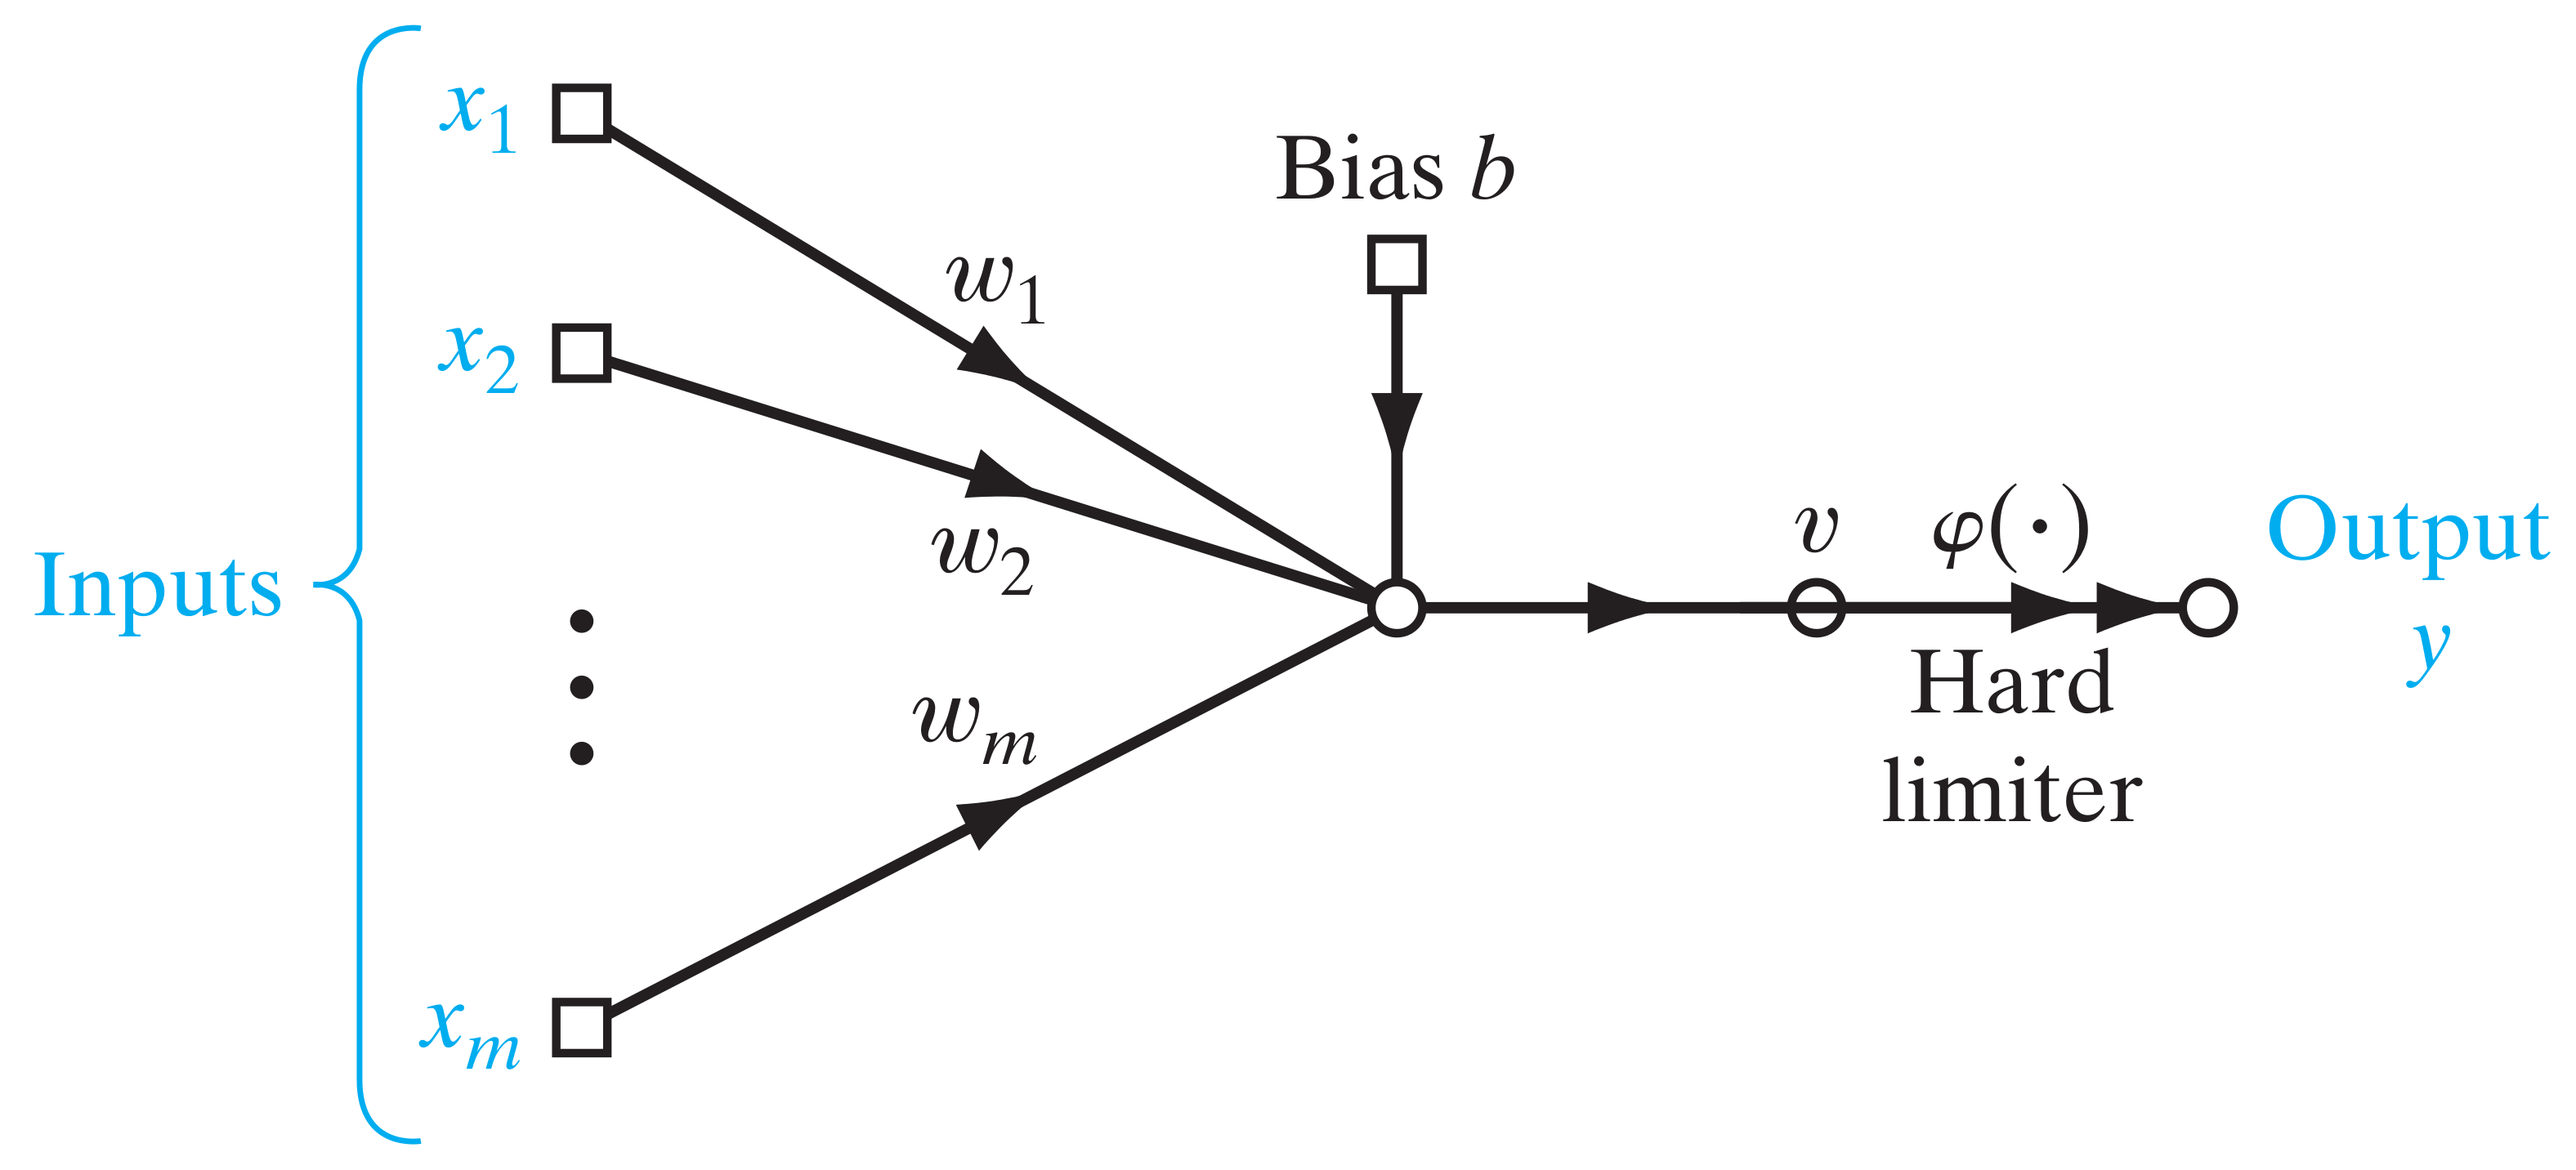
\includegraphics[width=.80\columnwidth]{images/064perceptron}
\caption[Perceptron scheme]{Perceptron scheme \cite{RefWorks:158}.}
\label{fig:064perceptron}
\end{figure}
In the simplest case  the activation function $\varphi(\cdot)$ is an hard
limiter, or a signum function.
Consequently, $y$ can be +1, for positive inputs, or -1, for negative inputs. Inputs of the first class
belong to class $\mathscr{C}_1$, of the second to class $\mathscr{C}_2$.
Thus, the patterns ($y$) are hypothesised to be linearly separable.
In this case the training, as identification of the correct weights and bias,
can be precisely mathematically described. \\
\begin{figure}[!h]
\centering
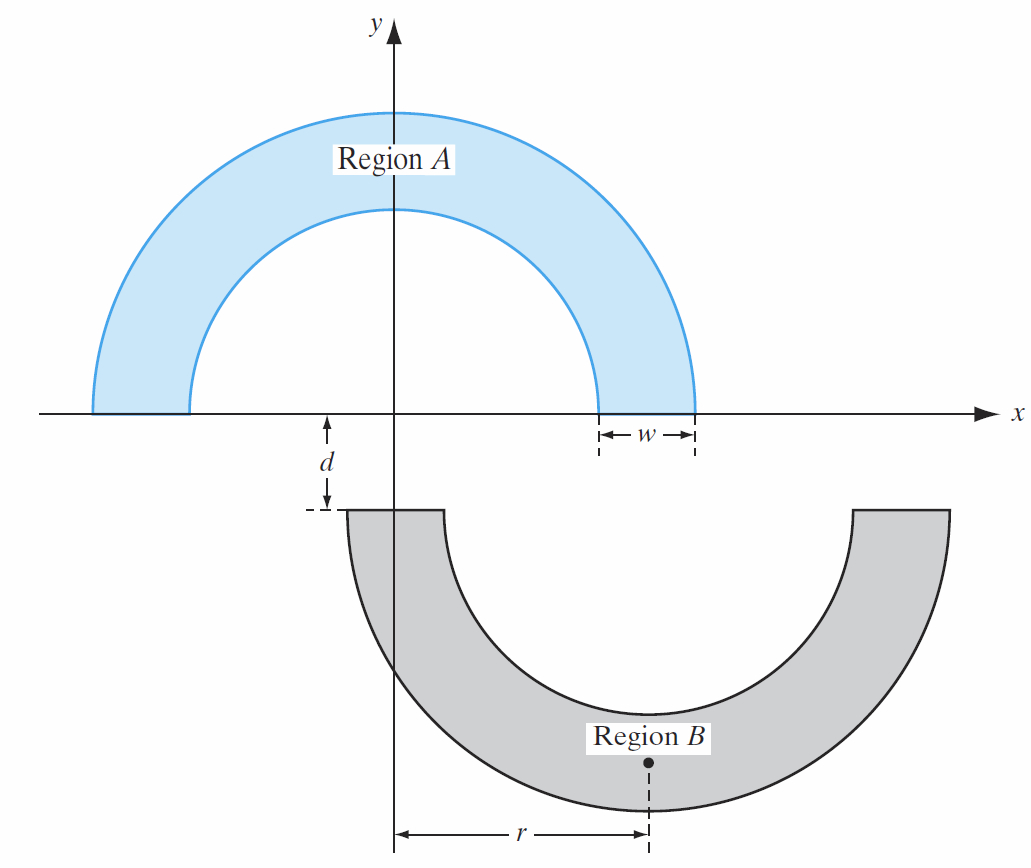
\includegraphics[width=.6\columnwidth]{images/105doublemoon2}
\caption[Double moon scheme]{Double moon scheme \cite{RefWorks:158}.}
\label{fig:105doublemoon2}
\end{figure}
The classical example of the double moon, see Fig. \ref{fig:105doublemoon2},
which clarifies the limits of the single perceptron approach, especially 
why a single neuron is not capable to handle a
nonlinear problem.
We drew two \textit{moons}, both with an inner radius $r$. 
Their minimum distance is $d$.
We could consider the two moons as composed by a finite number of
two-dimensional points.
If we use a portion of these points to train the $perceptron$, i.e. 
to teach the network which points belong to a region and which belong to the
other.
Goal of the $perceptron$ is to divide the two-dimensional
into two separate regions.
As long as $d$ is positive, the investigation space
can easily be linearly separated in two regions.
Once trained, the $perceptron$ can assign the remaining points 
to one moon or the other according to the training.

\section{Multilayer}
\label{sec:multilayer}

\begin{figure}[!h]
\centering
\includegraphics[width=.70\columnwidth]{images/063doublemoon}
\caption[Double moon classification problem 1]{Double moon classification
problem \cite{RefWorks:158}. Literature challenge to distinguish between linear
and non linear separation algorithms.}
\label{fig:063doublemoon}
\end{figure}



The handling of multiple outputs or, in our example, 
when $d$ becomes negative, see Fig. \ref{fig:063doublemoon}, makes linear
separation not possible, and a multineuron approach necessary. 
\wrong{better explanation of the example necessary}
\begin{figure}[!htb]
\centering
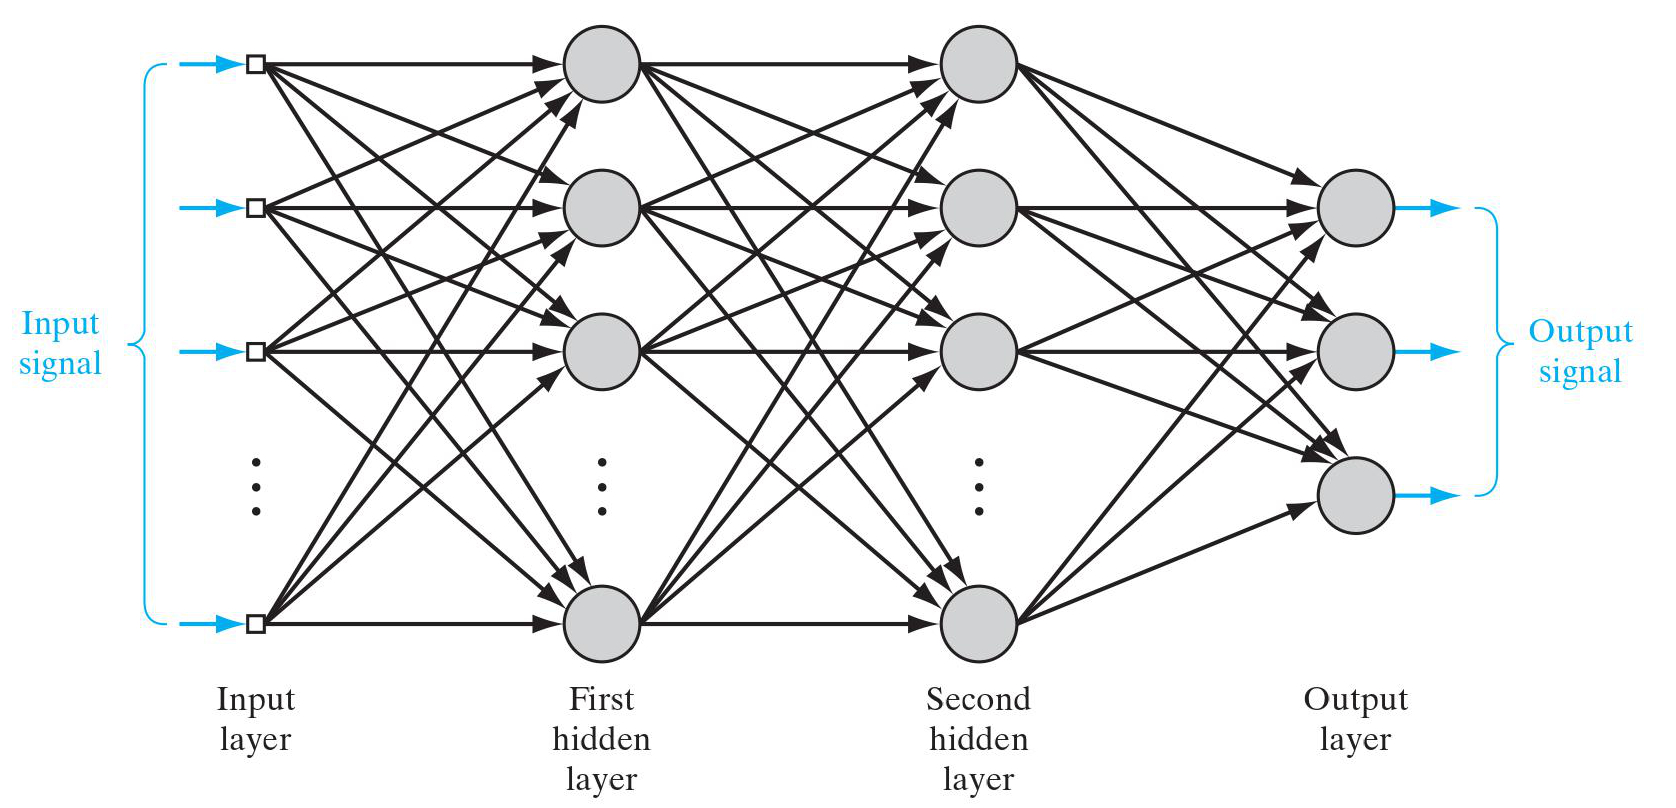
\includegraphics[width=.80\columnwidth]{images/111multilayerperceptron}
\caption[Multilayer perceptron]{Multilayer perceptron architecture, with
emphasys over the componing layers
\cite{RefWorks:158}.}
\label{fig:111multilayerperceptron}
\end{figure}
Many neurons are combined to form a network, as in the architecture presented
in Fig. \ref{fig:111multilayerperceptron}.
The first requirement of a multilayer neural network
is that each neuron of the network must have differentiable nonlinear activation
function, such as the strictly increasing hyperbolic tangent.
Further, the network must have at least one layer $hidden$ from both the input
and the output nodes, see Fig. \ref{fig:018nnscheme}, to compute higher-order
statistics.
An high degree of $connectivity$ is another salient characteristic, dependent on
the synaptic weights of the network.
Usually, each neuron of one layer is linked with all the neurons in the previous
layer.
A network is called \acs{FF} if the inputs of the neurons in
one layer are exclusively the output signals of the neurons in the previous
layer.\\

%\improvement{Add some more details about the multilayer from Haykin}
%\improvement{explain feed forward here, pag 21 haykin}

\section{Batch Learning}
\label{sec:batchlearning}

A Multilayer \acs{ANN} can be trained in a supervised fashion with a training
sample
\begin{equation}
\label{eq:trainingsample}
\mathscr{T} = \{\mathbf{x}(n), \mathbf{d}(n) \}^N_{n = 1},
\end{equation}

where $\mathbf{x}(n)$ is the stimulus applied to the input layer.
The error is calculated 
as the difference at the j-th
node between the output of the neuron ($y_j(n)$) and the expected response
($d_j(n)$):
\begin{equation}
\label{eq:error}
e_j(n) = d_j(n) - y_j(n).
\end{equation}

$\mathbf{d}(n)$ is the desired response vector, and $d_j(n)$ is its j-th
element.
As in the Least Mean Square algorithm (see \citet{RefWorks:158}), we define
the \textit{instanteneous error energy} for the j-th neuron as:
\begin{equation}
\label{eq:insterrorenergy}
\mathscr{E}_j(n) = \frac{1}{2}
\mathit{e}_j^2(n).
\end{equation}

If we sum over all the neurons in the output layer, we obtain
the \textit{total instanteneous error energy} as:
\begin{equation}
\label{eq:totalinsterrorenergy}
\begin{align*}
\mathscr{E}(n) & = \sum_{j \in C}{\mathscr{E}_j(n)} \\
			   & = \frac{1}{2} \sum_{j \in C}{\mathit{e}_j^2(n)}
\end{align*}
\end{equation}

With a total of $N$ expected
responses for training the cost function to be minimized can be expressed as the
\textit{error energy averaged over the training sample}:
\begin{equation}
\label{eq:costfunction}
\mathscr{E}_{av}(N) = \frac{1}{N}
\sum_{n=1}^{N}{\mathscr{E}_n(N)}.
\end{equation}


\section{Backpropagation algorithm}
\label{sec:backpropagationalgorithm}

% If we consider a single perceptron, each example consists of a vector of inputs
% and a scalar expected response.

A multilayer perceptron network can be trained with the
supervised back-propagation algorithm, composed of two phases, forward and
backward, as shown in Fig. \ref{fig:112ffbp}.
\begin{figure}[!htb]
\centering
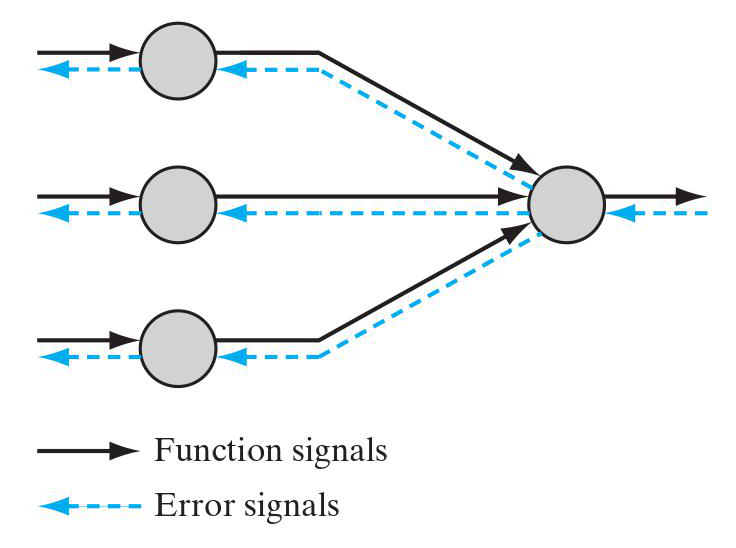
\includegraphics[width=.50\columnwidth]{images/112ffbp}
\caption[\acs{FF} Backpropagation]{\acs{FF} Backpropagation
\cite{RefWorks:158}.}
\label{fig:112ffbp}
\end{figure}
In the first phase the weights do not change. 
From the inputs through the hidden
and output layers the output is computed.
In the second phase the error is calculated 
and used to tune the weights, backward from the output to hidden
layers.
Of course, it arises the problem of when stopping the loop (or epoch). 
Thus, a cost
function (\acs{EW}) is defined: 
in each loop of
the algorithm its value is lower than in the previous loop.
If we consider $C$ neurons in the output layer the 
\textit{total instantaneous error energy} of the whole network is:
\wrong{rephrase after missing paragraph}
Consequently, the weight of the $i$-th input for the $j$-th neuron with the
$n$-th example is corrected as follow:
\begin{equation}
\label{eq:deltaweight}
\Delta w_{ji}(n) = -\eta \frac{\partial \mathscr{E}(n)}{\partial
\mathit{w}_{ji}(n)},
\end{equation}

where \acs{eta} is the \textit{learning-rate parameter},
which could be a user tuned parameter. 
A large \acs{eta} makes the algorithm fast,
while a small one prevents divergence.
Converged is reached when $\mathscr{E}_{av}(N) < 10^{-4}$.\\
The validity of the \textit{\acs{FF} Multilayer Perceptron Neural Networks}
(\acs{MLPNN}), with a backpropagation reinforcement learning training algorithm,
% (scaled conjugate gradient)
has been demonstrated in the 
literature, see \citet{RefWorks:158}. Several scientists 
\cite{RefWorks:161, RefWorks:166, RefWorks:167, RefWorks:168, RefWorks:169,
RefWorks:170, RefWorks:178, RefWorks:179} have employed \acs{ANNs} to model
the mechanical properties of materials.

\section{Optimization}
\label{sec:optimization}

Expanding this vision to multineurons network shifts into a matrix of inputs and
a vector of expected responses and consequently a vector of errors, from which
we can derive an error surface. Its local \textit{gradient vector}
\textbf{g}(\textit{n}) can be written as:

\begin{equation}
\label{eq:gradientvector}
\mathbf{g}(\mathit{n}) = 
\left. \frac{\partial \mathscr{E}_{av}(\mathbf{w})}{\partial
\mathbf{w}}\right|_{\mathbf{w}=\mathbf{w}(\mathit{n})} ,
\end{equation}

\wrong{insert the equation system}
The quadratic approximation of the error surface can be performed with the
following methods:

\begin{itemize}
  \item{conjugate gradient,}
  \item{Newton and quasi-Newton,}
  \item{Levenberg-Marquardt.}
\end{itemize}

Compared to a linear approximation the conjugate gradient method is 
more precise. 
Further, it is faster and less computationally demanding than the
remaining quadratic methods.
First, the weights are randomly initialized. 
At every iteration the n-th example is used to computed $\eta$, and later
explicetely the weights $(n + 1)$'th iteration are obtained.
Then \textbf{g}(\textit{n + 1}) is calculated, to be later used with the
Polak-Ribiere method to compute the direction vector.
The gradient methods stops when the residuals, calculated from the
\acs{EAVN}, reach convergence.

% To be able to handle non-linearly separable data, the standard linear perceptron
% \acs{ANN} was modified to obtain \textit{FF Multilayer Perceptron Neural Networks
% (MLPNN)}.
% Here, each processing unit or node (neuron) possesses a nonlinear activation function. 
% They are interconnected to form layers that are also interlinked. 

\section{Generalization}
\label{sec:generalization}

\begin{figure}[htbp]
  %\null\hfill
  \subfloat[Good fitting.]{
	  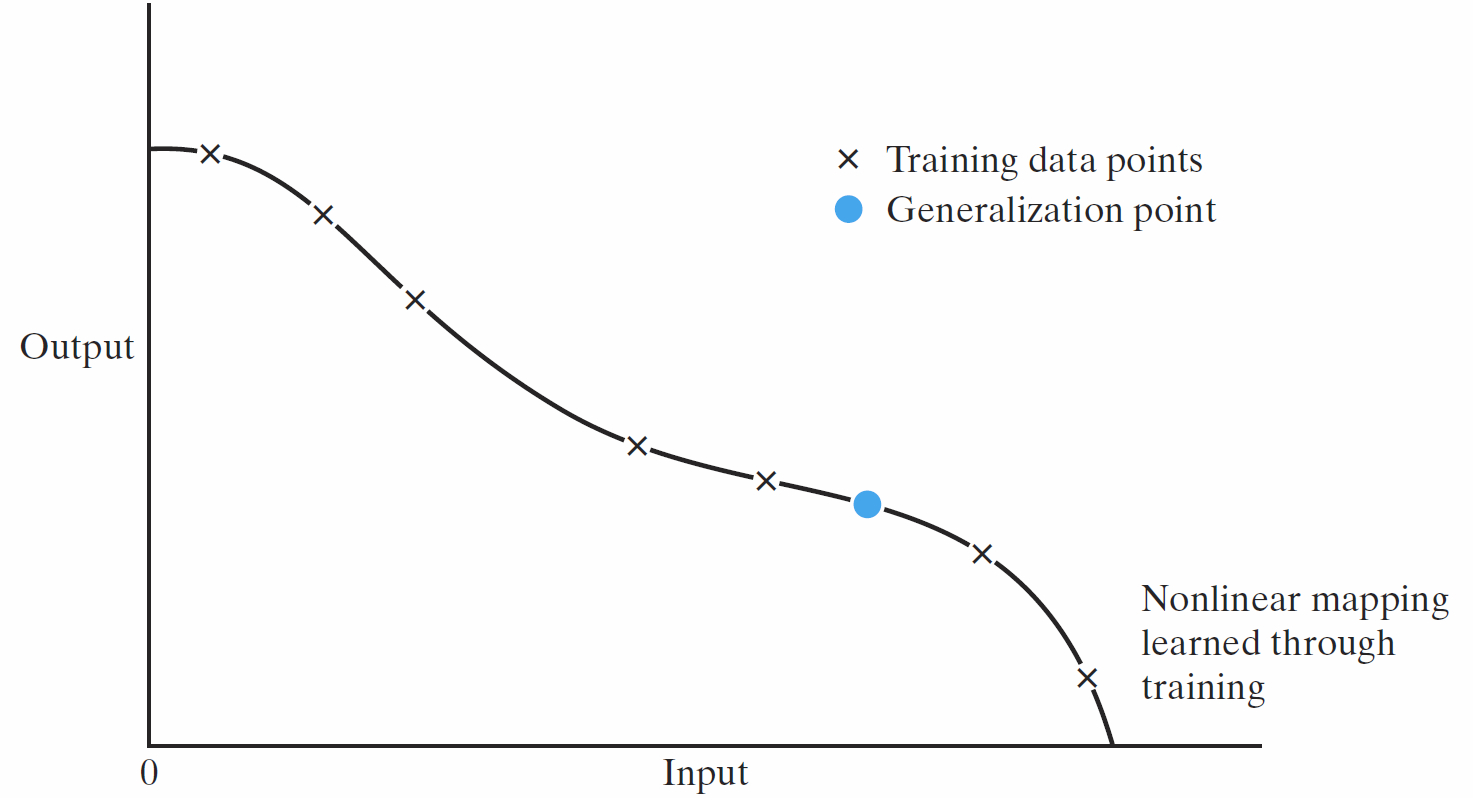
\includegraphics[width=.47\columnwidth]{images/106goodfitting}
	  \label{fig:106goodfitting}  }
  \quad
 % \hfill
  \subfloat[Bad fitting.]{
	  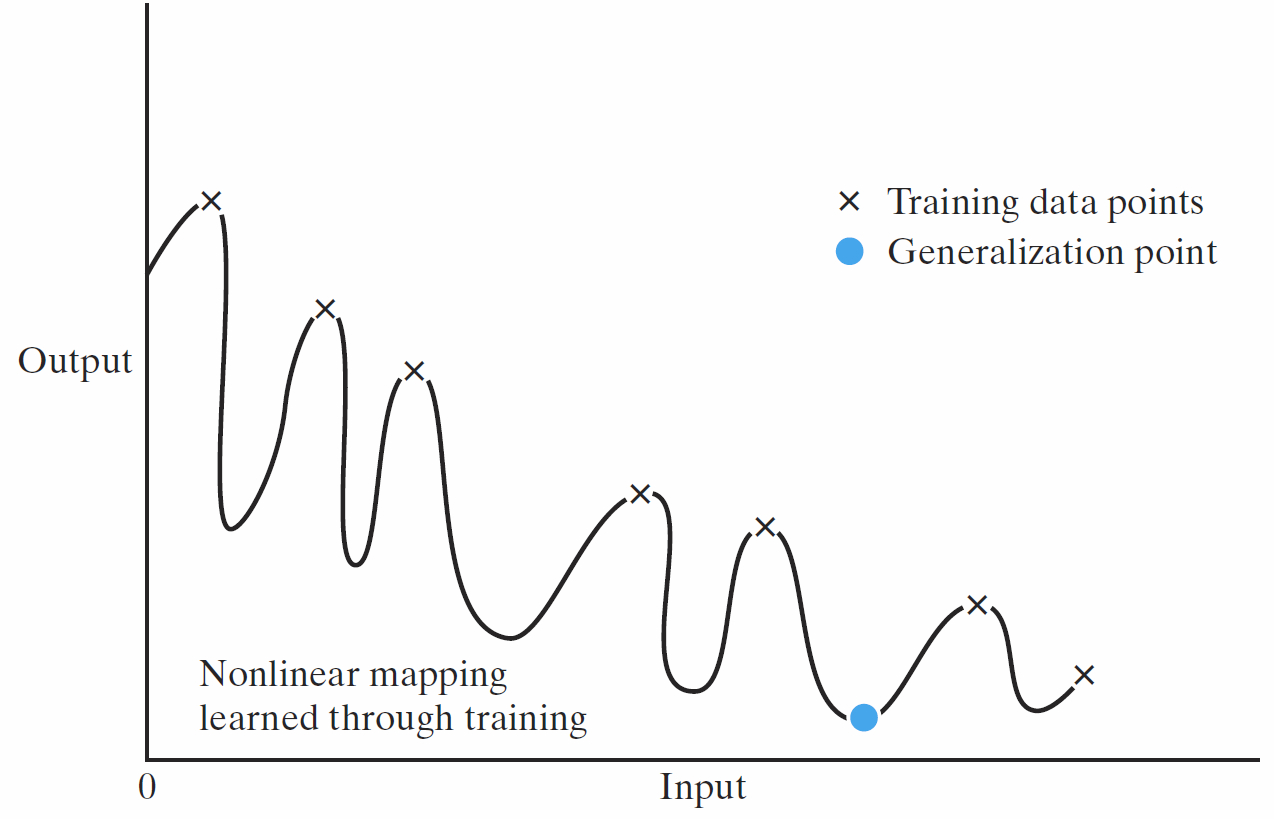
\includegraphics[width=.47\columnwidth]{images/107badfitting}
	  \label{fig:107badfitting}
  }
 % \hfill\null
  \caption[Fitting.]{Fitting, or agreement, between data point and
  regression, or interpolation, functions
  \cite{RefWorks:158}.}
  \label{fig:108fitting}
\end{figure}

Correctly computed input-output mapping is a synonym of a well $generalized$
network, and of good nonlinear interpolation of the inputs, as in Fig. 
\ref{fig:106goodfitting}. On the other hand, an excessive amount of
training samples, known as $overfitting$, leads to poor generalization, see 
Fig. \ref{fig:107badfitting}. Also the architecture of the neural network and
physical complexity of the problem influence the generalization.
A good rule of thumb requires the size of the training sample to be of the same
order of magnitude of the ratio between (a) the total number of free parameters 
(i.e., synaptic weights and biases) in the
network and (b) the fraction of classification errors permitted on test
data (e.g., the mean square value of the estimation error).

\begin{table}[htbp]
  \centering

    \begin{tabular}{l|ccc}
    \hline
          & Bayesian & Gaussian & ANN \\
          \hline
    Cost function & maximum  & maximum & scaled \\
     			  & likelihood & likelihood & conjugated \\
     			  & estimation & estimation & gradient \\
    \hline
    \end{tabular}%
      \caption{Regression methods comparison.}
  \label{tab:17regressionmethods}%
\end{table}%

\section{Cross validation}
\label{sec:crossvalidation}

A computationally efficient training and the evaluation of good generalization
can be performed with the statistical tool of \textit{cross-validation}.
The available data are randomly divided in the following subsets:

\begin{enumerate}
  \item{training samples subset,}
  \item{generalization (or validation, or early stopping) samples subset,}
  \item{test samples subset.}
\end{enumerate}

For instance, every ten epochs the training is halted and the validation error
(or the cost function) is evaluated with the partially trained network over the
validation set.
Then the training is resumed.
This continues until the learning curve of the error for the validation set
reaches a local minimum, a condition that should happen sooner (i.e., in a
minor number of loops) than the falling of the learning curve for the training
set (cost function \acs{EAVN}) under the prescribed limit.
At this point the output of the trained network is evaluated over the test
subset to evaluate its generalization performances.
Also the standard regression models (i.e., Bayesian and Gaussian) are similarly
evaluated.

\section{ANNs training for DEM identification}
\label{sec:annstrainingfordemidentification}

Following the best practice suggested by \citet{RefWorks:150}, we
used $MLPNN$.
Further, the quality of the \acs{ANN} data had to be examined critically. 
\citet{RefWorks:158} 
suggested considering the quality of (a) \acs{ANN} training process and (b) the
subsequent data generation based on the inputs provided.
Task (a) is particularly important
when dealing with experimental training data, and
usually addressed
by noise-corrupted pattern calibration
and by comparison with standard statistical methods.
However, our training pool was numerical and extensive, 
and the particles in our simulations were inserted using a random
seed value.
For vast amounts of training data, the effect of noise-corrupted patterns is
negligible, see \citet{RefWorks:158}.
Thus, in our work task (b) was more challenging.
Once trained, the \acs{ANN} were fed
combinations of \acs{DEM} parameters. 
We tried different methods to generate these combinations. 
Our first attempt consisted of assigning parameters to the investigated
variables in even increments from the minimum to the maximum values. 
For example, the \acs{CoR} ranged from 0.5 to 0.9, and thus the first value was
0.5, the second 0.508163, and so on.
To increase generalization, we decided to follow a different approach: 
random value generators created the number of required values in the defined
ranges for each parameter investigated.
These were combined and used as input.\\

% !TEX encoding = UTF-8
% !TEX TS-program = pdflatex
% !TEX root = ../Tesi.tex
% !TEX spellcheck = en-EN

%************************************************
\part{Identification of DEM parameters}
\label{par:identification}
%************************************************

\lipsum[1]



% !TEX encoding = UTF-8
% !TEX TS-program = pdflatex
% !TEX root = ../Tesi.tex
% !TEX spellcheck = it-IT

%************************************************
\chapter{Numerical Simulation}
\label{cap:numericalsimulation}
%************************************************

\lipsum[1]


\section{Angle of Repose}
\label{sec:aorsim}


\lipsum[1]


\section{Shear Cell}
\label{sec:scsimulation}
%************************************************

\lipsum[1]

% !TEX encoding = UTF-8
% !TEX TS-program = pdflatex
% !TEX root = ../Tesi.tex
% !TEX spellcheck = it-IT

%************************************************
\chapter{Experimental Characterization}
\label{cap:experimentalcharacterization}
%************************************************

\lipsum[1]



\section{Particle Distribution}
\label{sec:particledistribution}

\lipsum[1]



\section{Angle of Repose (p-p) - Small Scale}
\label{sec:aor}


\lipsum[1]

\section{Angle of Repose (p-p) - Large Scale}
\label{sec:aorlargescale}


\lipsum[1]



\section{Schulze Ring Shear Cell tester (p-p)}
\label{sec:SRSCT}
%************************************************

\lipsum[1]

\section{Jenike Shear Cell tester}
\label{sec:jsct}
%************************************************

\lipsum[1]
% !TEX encoding = UTF-8
% !TEX TS-program = pdflatex
% !TEX root = ../Tesi.tex
% !TEX spellcheck = en-EN

%************************************************
\chapter{Artificial Neural Network Generalization}
\label{cap:anntraining}
%************************************************

\section{Principal Component Analysis (PCA) Results}
\label{sec:pcaanalysis}

We evaluated the linear relationship between the microscopic and the
macroscopic parameters in the training simulations with Matlab Principal
Component Analysis.
The results can be seen in Table \ref{tab:06inputRelationshipTable}.
Sliding friction (\acs{mus}), rolling friction (\acs{mur}) and particle density (\acs{rhop})
had the greatest influence on, respectively, the coefficient of pre-shear
(\acs{mupsh}), the angle of repose  (\acs{AoR}) and the bulk density (\acs{rhob}). Notably, \acs{rhop}
was not used as a training parameter for \acs{AoR} bulk behaviour. \\
In fact, we can see how each relationship is below the 100\% necessary to claim
a direct linear correlation.
Thus, we demonstrated that we need more precise statistical tools to investigate
the relationships and generalize the results.

\begin{table}[h]
\centering
\scalebox{1.0}{
\begin{tabular}{c|cccccccc}
\hline
          & $\mu_s$ & $\mu_r$ & $COR$ & $\rho_p$ & $\mu_{sh}$ & $\mu_{psh}$ & $\rho_{b}$ & $AOR$ \\
          \hline
    $\mu_s$ & 100.00 & 0.55  & 0.04  & 0.00  & 3.84  & 87.26 & 8.39  & 49.48 \\
    $\mu_r$ & 0.55  & 100.00 & 0.15  & 0.00  & 58.92 & 33.70 & 3.10  & 60.20 \\
    $COR$ & 0.04  & 0.15  & 100.00 & 0.00  & 15.52 & 0.57  & 1.71  & 0.00 \\
    $\rho_p$ & 0.00  & 0.00  & 0.00  & 100.00 & 4.98  & 5.71  & 99.00 & 0.00 \\
    $\mu_{sh}$ & 3.84  & 58.92 & 15.52 & 4.98  & 100.00 & 26.03 & 9.52  & 0.00 \\
    $\mu_{psh}$ & \textbf{87.26} & 33.70 & 0.57  & 5.71  & 26.03 & 100.00 & 4.33 
    & 0.00
    \\
    $\rho_{b}$ & 8.39  & 3.10  & 1.71  & \textbf{99.00} & 9.52  & 4.33  & 100.00
    & 0.00 \\
    $AOR$ & 49.48 & \textbf{60.20} & 0.00  & 0.00  & 0.00  & 0.00  & 0.00  &
    100.00 \\
    
\hline
\end{tabular}}
\caption{Values of linear relationship between considered variables multiplied
for 100}
\label{tab:06inputRelationshipTable}
\end{table}

\section{Regression statistic training concept}
\label{sec:regressiontrainingconcept}

\begin{figure}[!htb]
\centering
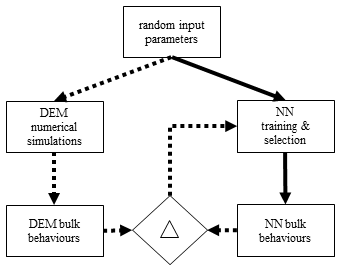
\includegraphics[width=.50\columnwidth]{images/127anntraining}
\caption[ANN training]{ANN training.}
\label{fig:127anntraining}
\end{figure}

Initially, as shown in Fig. \ref{fig:019methodology} in the training phase
(dashed lines) \acs{DEM} simulations are performed
with random initial input parameters.
The behaviours obtained are used to train the following regression models:
\begin{itemize}
  \item{Bayesian linear,}
  \item{Gaussian non linear,}
  \item{Artificial Neural Network (\acs{ANN}).}
\end{itemize}
For all the three models training consists in a loop that continues until the
difference between the outputs of each model and its samples is below the
limit ($\Delta$) (see Chapter \ref{cap:ann} for more details).\\
Thus, we were able to use the \acs{DEM} parameter combinations and their
corresponding bulk values to train the models.
Especially, we divided the samples in three pools: the first, with 70\% of the
samples, as \textit{training set}, the second, with 15\% of the samples, as
\textit{generalization set}, for early stopping, and the third, as \textit{test
set}, as suggested by Haykin (2009). The assignment of each sample to each pool
was random.

\subsection{ANN training concept specifications}
\label{subsec:anntrainingconceptspecifications}

The training of an \acs{ANN} consists in defining the weights and the biases for
each of its neuron.
We first defined the typology of Artificial Neural Networks (\acs{ANNs}) we used and
the input we fed them, see Benvenuti et al. \cite{RefWorks:205}.
Our \acs{ANNs} have three different layers: the input layer has a number of neurons
equal to the number of different inputs of the network, see Fig.
\ref{fig:018nnscheme}, with the scheme of how the Multilayer Perceptron \acs{ANN} ($MLPNN$) derives one
bulk-behaviour-dependent variable from the mutually independent simulation variables.
The hidden (or central) layer's number of neurons was to be investigated. 
The output layer contains one neuron for the output.
The transfer function for the neurons of the central layer is the tangential
sigmoid, while the neuron of the output layer use the linear transfer
function.\\
\begin{figure}[!htb]
\centering
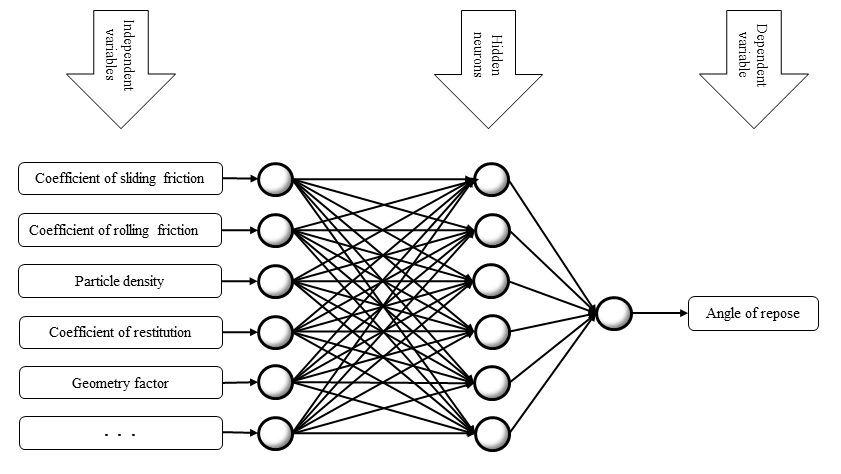
\includegraphics[width=.96\columnwidth]{images/129NN22}
\caption[ANN Scheme]{Artificial Neural Network (\acs{ANN}) Scheme. Regressors
are show in the left-hand side of the image. An example of a response is shown
in the right-hand side of the image.}
\label{fig:018nnscheme}
\end{figure}
We started with all the \acs{DEM} parameter combinations and their corresponding
numerical \acs{mupsh} from the \textit{training set} to create 36 \acs{ANNs} that
differed in their numbers of neurons in the hidden layer (between five to forty neurons).
The \textit{generalization set} was used to speed the training. 
We then determined the coefficient of determination (\acs{r2}), 
\begin{equation}
R^2 = \frac {SSR}{SST} = 1 - \frac {SSE}{SST} .
 \label{eq:rsquare}
\end{equation}

between the
$bulk-macro$ behaviours in the output of the \acs{ANN} and the \textit{test
set} simulations, which were not correlated with the remaining 70\% used for the
training.
Thus, we could select for \acs{mupsh} the \acs{ANN} with the maximum \acs{r2}, 
again as suggested by Vaferi et al. \cite{RefWorks:150}, and we noted its number
of neurons.
We repeated the same \acs{ANN} creation steps for \acs{mush}, \acs{rhob}
and \acs{AoR}, obtaining one trained \acs{ANN} for each bulk value. \\

\subsection{Sinter fine ANN training}
\label{subsec:sinterfineanntraining}

As said, we started with the sinter fine.
The first bulk value \acs{ANN} trained was the \acs{mupsh}, where we achieved a
$\acs{r2} = 0.96$ for an \acs{ANN} with twenty neurons, a consistent agreement
between the \acs{DEM} and the \acs{ANN} values, which demonstrates the accurate predictive power of
the \acs{ANN}, compared to the other two methods.
Increasing the number of neurons did not improve the \acs{r2}; it even started to
oscillate with higher numbers of neurons.
The weights and biases, which represent the trained network, can be be found in
Table \ref{tab:34weightsoriginalsinterfinesct}.
In Fig. \ref{fig:022regression} the corresponding plot for the \acs{ANN} with the maximum \acs{r2} is shown. 
Each circle represents one of the 546 simulations. \\
We subsequently obtained the optimal number of neurons for all
\acs{ANNs}. Table \ref{tab:35weightssinterfineaor} shows the weights for the
\acs{AoR}.\\

\begin{figure}[!h] 
\centering 
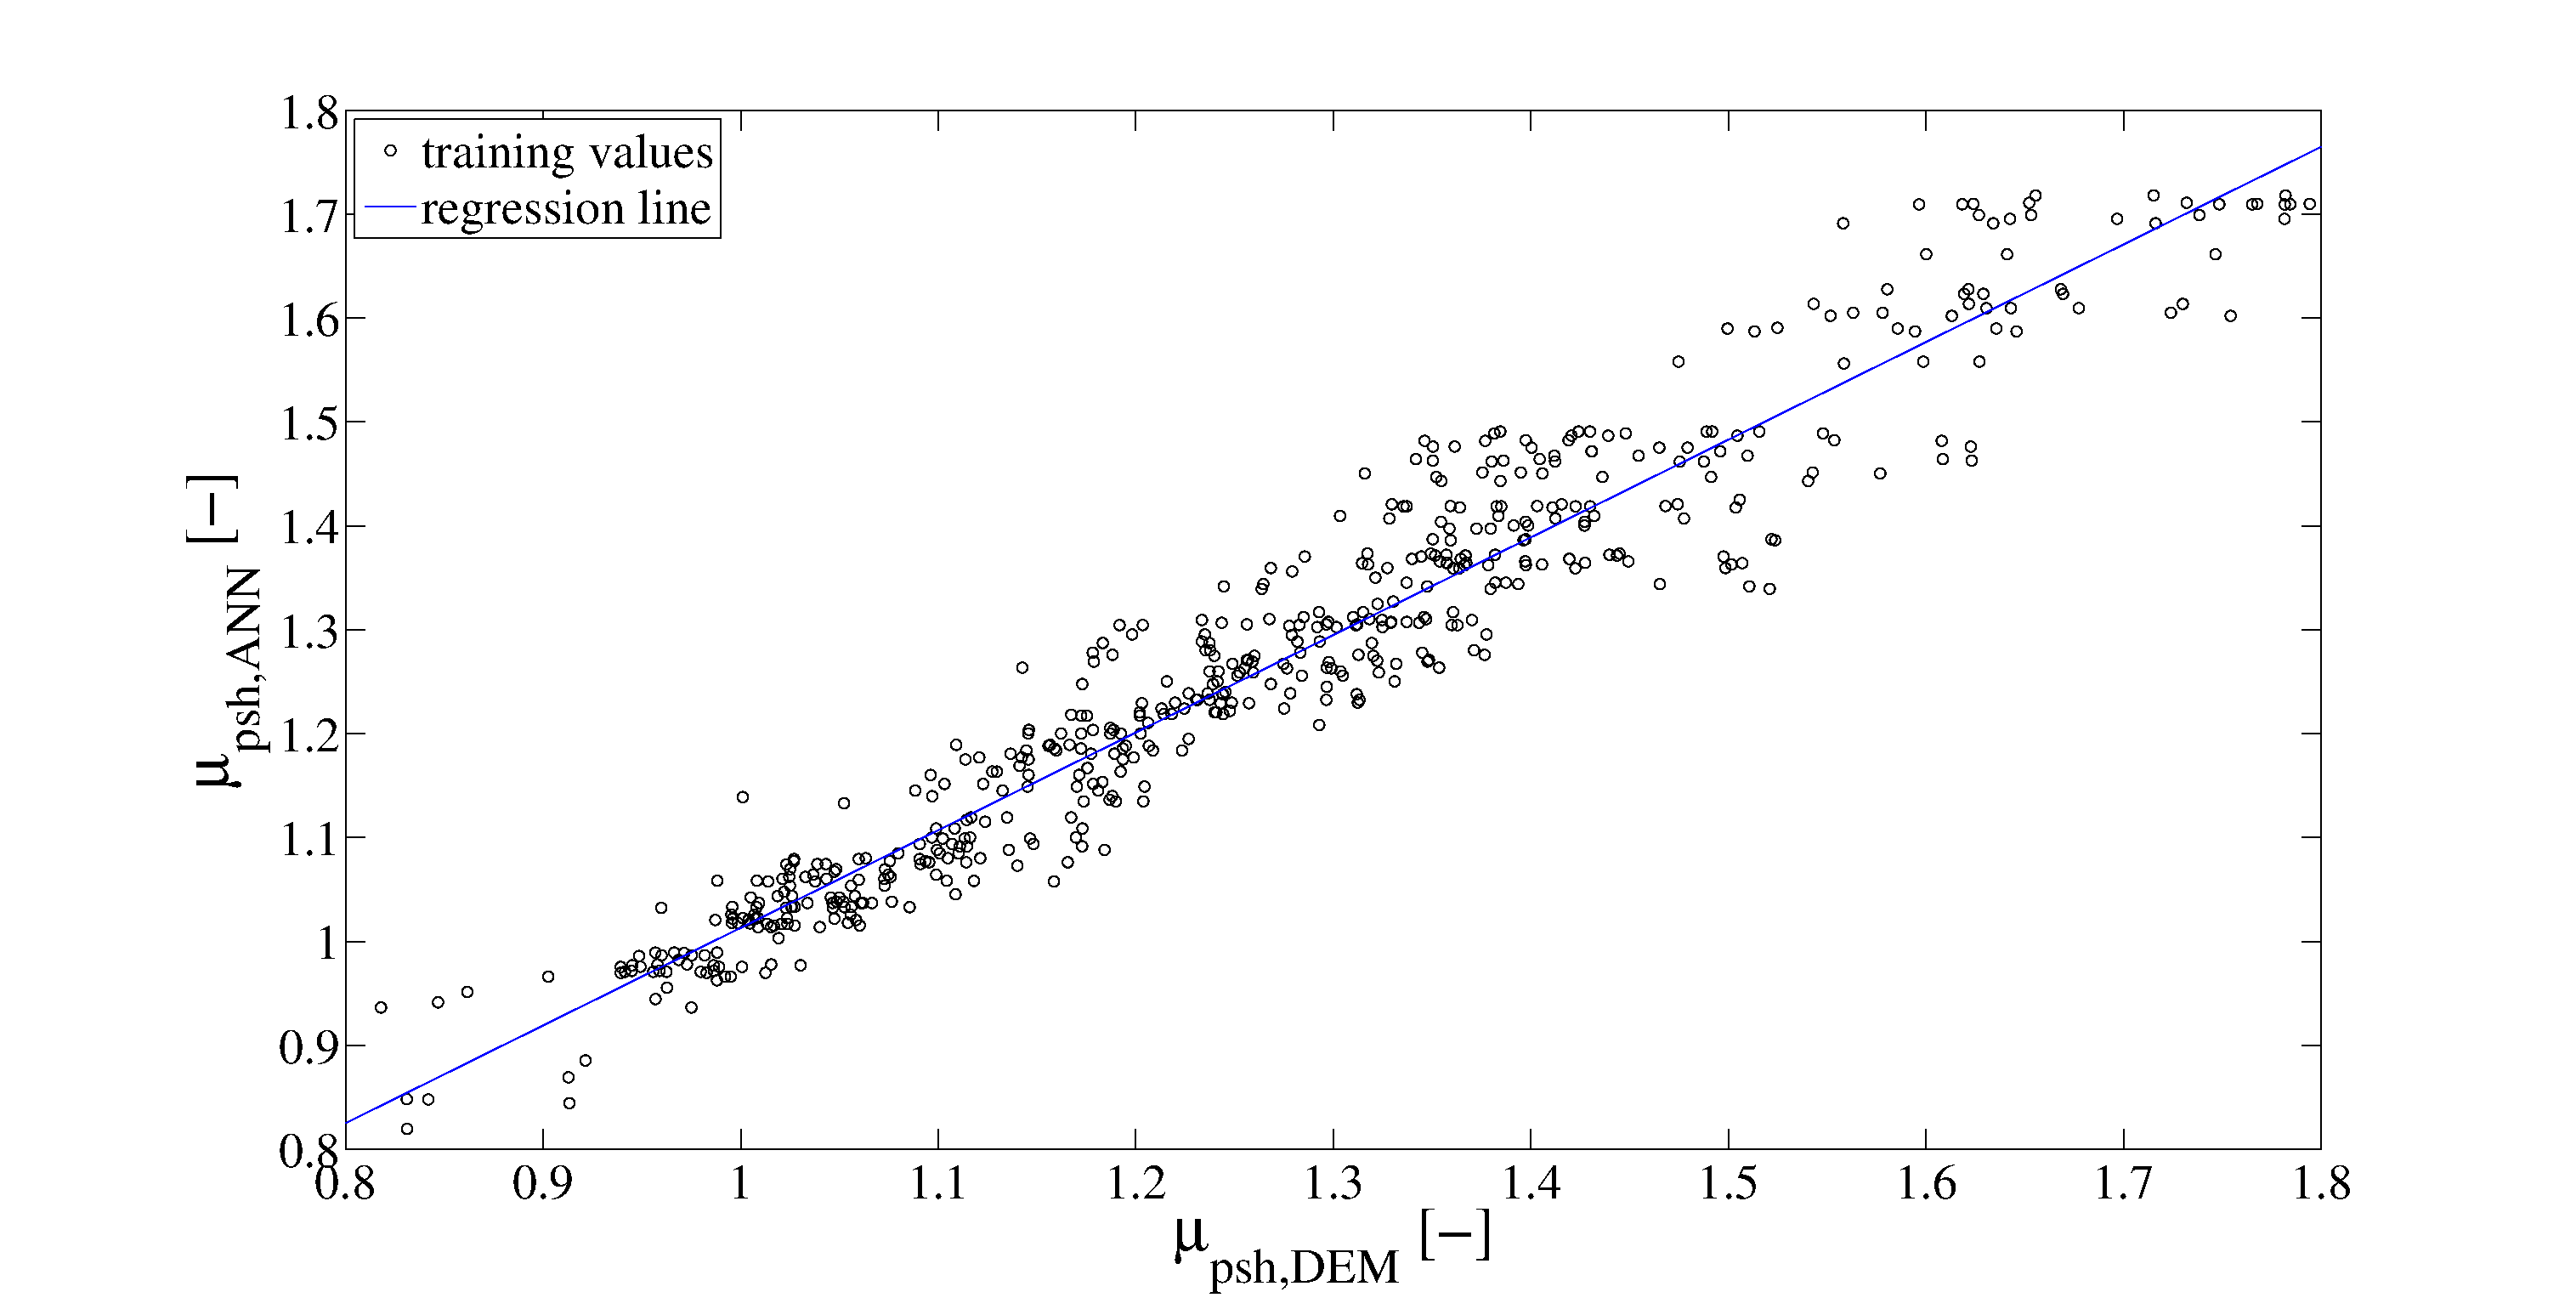
\includegraphics[width=.80\columnwidth]{images/022regression.eps}
%[width=.96\textwidth]
\caption[Comparison between prediction of the trained ANN and full DEM
simulation]{Comparison between prediction of the trained Artificial Neural
Network (\acs{ANN}) and 546 
\wrong{write down all the simulations performed at the end.}
full DEM simulations of the coefficient of pre-shear
(\acs{mupsh}).}
\label{fig:022regression} 
\end{figure}
\begin{table}[htbp] 
 \centering 
\begin{tabular}{l|cccccccccc} 
 \hline 
   &    \multicolumn{10}{l}{Weights of connection between input and hidden layer}  \\ 
 Neurons & 1 &  2 &  3 &  4 &  5 &  6 &  7 &  8 & 9 & 10 \\ 
 \hline 
  & 1.583 &  -0.543 &  -0.135 &  -0.462 &  1.370 &  1.048 &  1.025 &  -0.542 &  -0.162 &  -0.499 \\ 
  & -0.062 &  -0.576 &  -0.107 &  -1.246 &  -0.362 &  -0.239 &  1.078 &  1.156 &  0.161 &  0.919 \\ 
  & -0.057 &  0.265 &  0.552 &  -0.660 &  -0.006 &  1.021 &  0.139 &  -0.415 &  1.115 &  0.920 \\ 
  & 1.618 &  1.564 &  0.398 &  0.693 &  0.865 &  -0.047 &  0.535 &  -0.450 &  -0.558 &  -1.034 \\ 
  & 0.341 &  -0.028 &  -2.021 &  -1.331 &  0.899 &  -0.052 &  1.293 &  0.258 &  -1.550 &  0.786 \\ 
  & 0.309 &  0.682 &  0.277 &  -0.250 &  0.885 &  1.141 &  0.587 &  -0.825 &  -0.497 &  -0.054 \\ 
  & -0.186 &  0.950 &  -0.373 &  -0.218 &  0.355 &  -0.815 &  0.072 &  1.283 &  0.576 &  -0.740 \\ 
\hline 
   &    \multicolumn{10}{l}{Weights of connection between hidden and output layer}  \\ 
  & -0.200 &  -0.496 &  0.260 &  -0.210 &  0.061 &  0.023 &  0.202 &  0.033 &  0.079 &  0.167 \\ 
\hline 
   &    \multicolumn{10}{l}{Biases of hidden layer}  \\ 
  & -1.906 &  2.073 &  1.657 &  1.479 &  -1.280 &  -1.119 &  -0.770 &  0.569 &  0.345 &  -0.075 \\ 
\hline
\hline  
   &    \multicolumn{10}{l}{Weights of connection between input and hidden layer}  \\ 
 Neurons & 11 &  12 &  13 &  14 &  15 &  16 &  17 &  18 & 19 & 20 \\ 
 \hline 
  & -0.154 &  -0.126 &  -0.303 &  0.798 &  -1.191 &  -0.704 &  -0.254 &  -0.988 &  0.788 &  -0.612 \\ 
  & -0.292 &  0.715 &  1.266 &  -0.506 &  0.074 &  -1.095 &  -1.565 &  -1.085 &  -0.968 &  -0.073 \\ 
  & -0.443 &  1.142 &  0.342 &  -0.198 &  0.545 &  -0.202 &  0.722 &  -0.577 &  -1.573 &  -0.440 \\ 
  & 0.918 &  0.458 &  -1.031 &  -0.916 &  -0.092 &  0.312 &  0.935 &  -0.390 &  -0.489 &  -1.510 \\ 
  & -0.612 &  0.922 &  1.412 &  -0.305 &  -0.120 &  -0.696 &  -0.396 &  0.834 &  0.908 &  -0.022 \\ 
  & -1.047 &  -1.113 &  0.228 &  1.605 &  -0.899 &  -1.168 &  -0.017 &  -0.081 &  0.341 &  0.876 \\ 
  & -1.320 &  0.114 &  -0.233 &  -0.013 &  1.191 &  0.087 &  -0.527 &  1.106 &  0.266 &  0.877 \\ 
\hline 
   &    \multicolumn{10}{l}{Weights of connection between hidden and output layer}  \\ 
  & -0.082 &  0.173 &  -0.419 &  0.054 &  0.023 &  -0.056 &  -0.181 &  -0.150 &  0.167 &  -0.580 \\ 
\hline 
   &    \multicolumn{10}{l}{Biases of hidden layer}  \\ 
  & -0.231 &  -0.508 &  0.435 &  0.813 &  -1.221 &  -1.386 &  -1.356 &  -1.671 &  1.700 &  -2.221 \\ 
\hline 
\hline 
   &    \multicolumn{10}{l}{Biases of output layer}  \\ 
 &    \multicolumn{10}{c}{-0.543}  \\ 
\hline 
 \end{tabular} 
\caption[Weights and biases table for the coefficient of internal friction
for sinter fine]{Weights and biases table for the coefficient of internal
friction for sinter fine.}
\label{tab:originalsinterfinesct} 
\end{table}
\begin{table}[htbp] 
 \centering 
\begin{tabular}{l|ccccccccc} 
 \hline 
   &    \multicolumn{9}{l}{Weights of connection between input and hidden layer}  \\ 
 Neurons & 1 &  2 &  3 &  4 &  5 &  6 &  7 &  8 & 9 \\ 
 \hline 
  & 0.148 &  -0.064 &  -0.585 &  -1.247 &  1.264 &  0.108 &  -0.335 &  -0.950 &  0.722 \\ 
  & 1.889 &  1.334 &  -0.105 &  1.016 &  1.781 &  -0.652 &  -1.664 &  1.497 &  -0.578 \\ 
  & -0.271 &  1.221 &  1.086 &  0.777 &  0.298 &  0.984 &  0.101 &  -1.466 &  -0.230 \\ 
  & -1.316 &  0.385 &  -1.997 &  -1.531 &  -1.159 &  1.877 &  1.227 &  0.948 &  1.643 \\ 
\hline 
   &    \multicolumn{9}{l}{Weights of connection between hidden and output layer}  \\ 
  & 0.137 &  0.437 &  -0.575 &  -0.025 &  0.109 &  -0.667 &  -0.184 &  0.119 &  0.806 \\ 
\hline 
   &    \multicolumn{9}{l}{Biases of hidden layer}  \\ 
  & -2.453 &  2.311 &  1.399 &  0.679 &  0.108 &  0.844 &  -1.614 &  -1.674 &  2.654 \\ 
\hline 
   &    \multicolumn{9}{l}{Biases of output layer}  \\ 
 &    \multicolumn{9}{c}{-0.494}  \\ 
\hline 
 \end{tabular} 
\caption[Weights and biases table for sinter fine AoR]{Weights and biases table
for sinter fine \acs{AoR}.}
\label{tab:35weightssinterfineaor} 
\end{table}

\section{Statistical tools comparison}
\label{sec:statisticaltoolscomparison}

%\begin{figure}[htbp]
  %\null\hfill
  \subfloat[SCT Bayesian linear regressor.]{
	  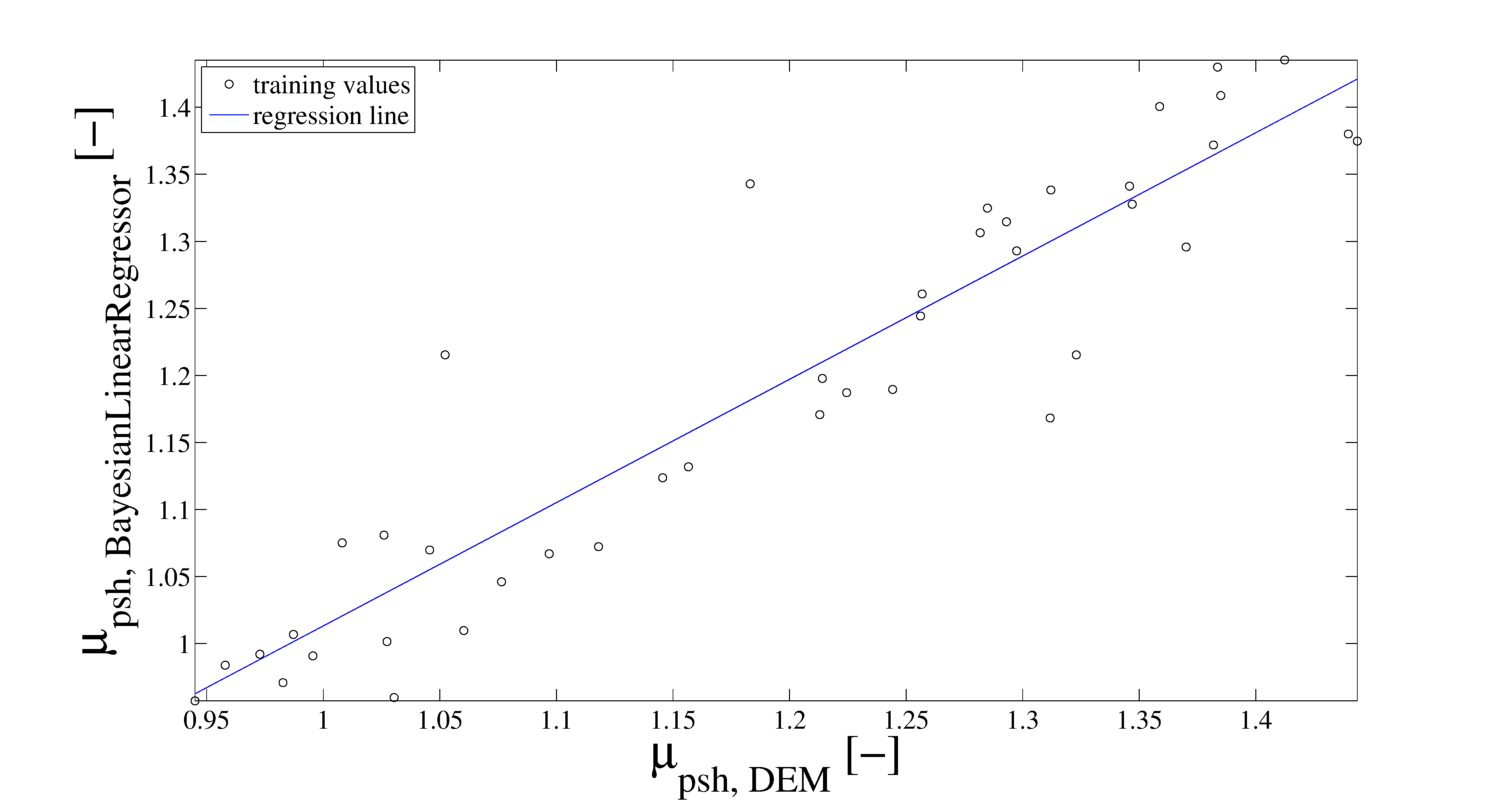
\includegraphics[width=.48\columnwidth]{images/069sctbayesianlinearregressor}
	  \label{fig:069sctbayesianlinearregressor}
  }
  \quad
    \subfloat[SCT Gaussian non linear regressor.]{
	  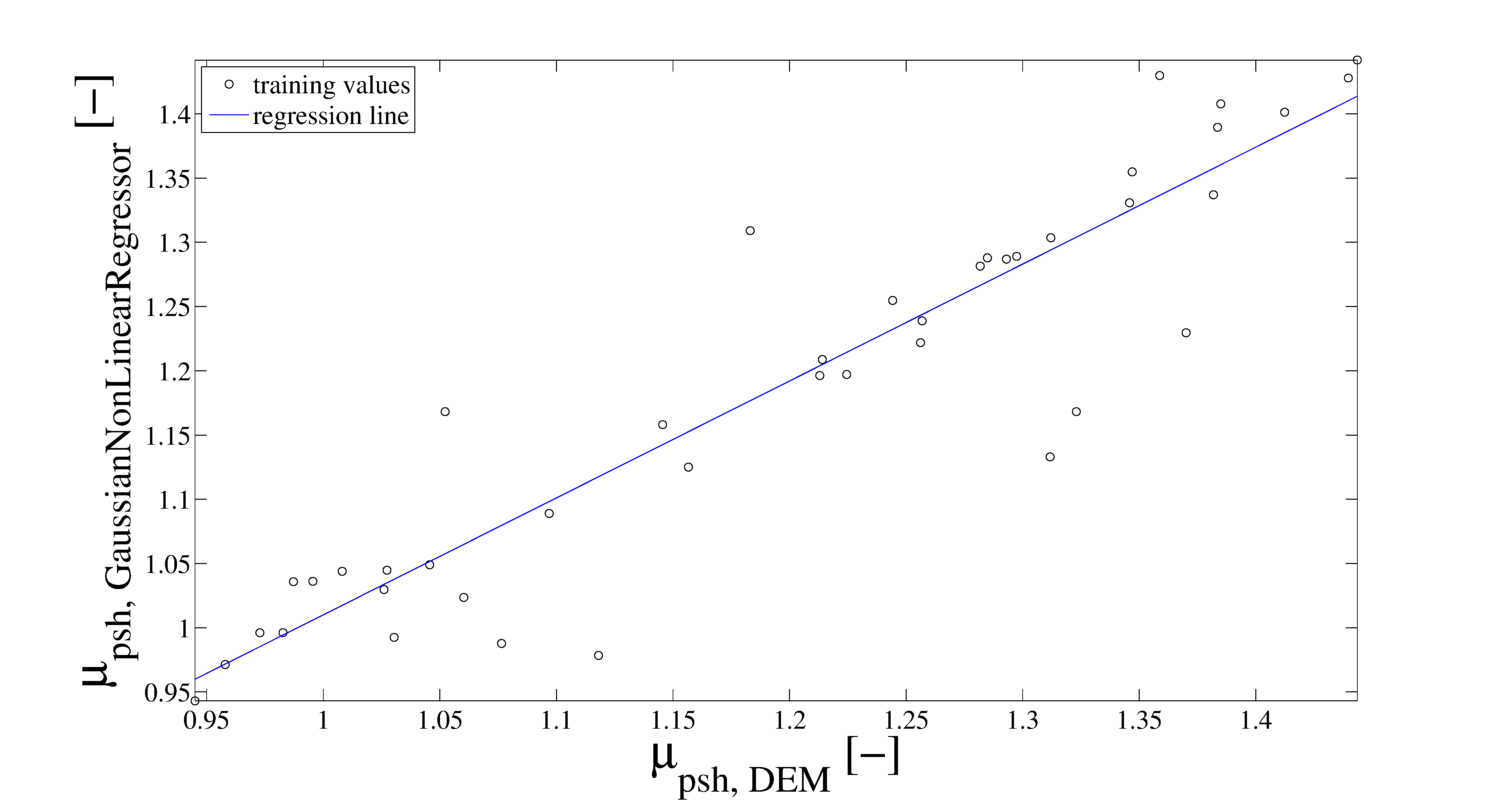
\includegraphics[width=.48\columnwidth]{images/070sctgaussiannonlinearregressor}
	  \label{fig:070sctgaussiannonlinearregressor}
  }
  \\
 % \hfill
  \subfloat[SCT ANN non linear regression.]{
	  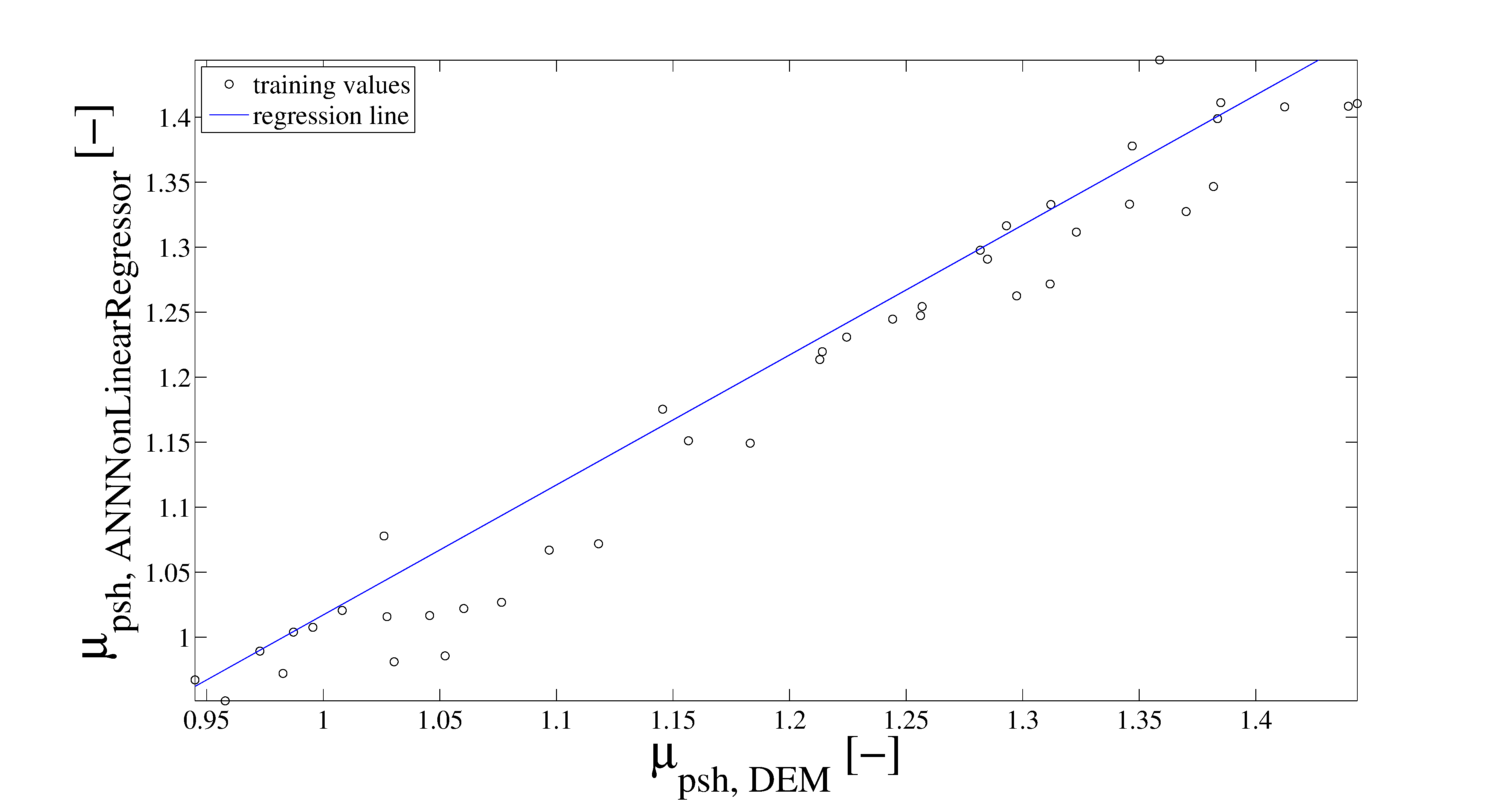
\includegraphics[width=.48\columnwidth]{images/071annnonlinearregressor}
	  \label{fig:071annnonlinearregressor}
  }
  \quad
    \subfloat[AoR Bayesian linear regressor.]{
	  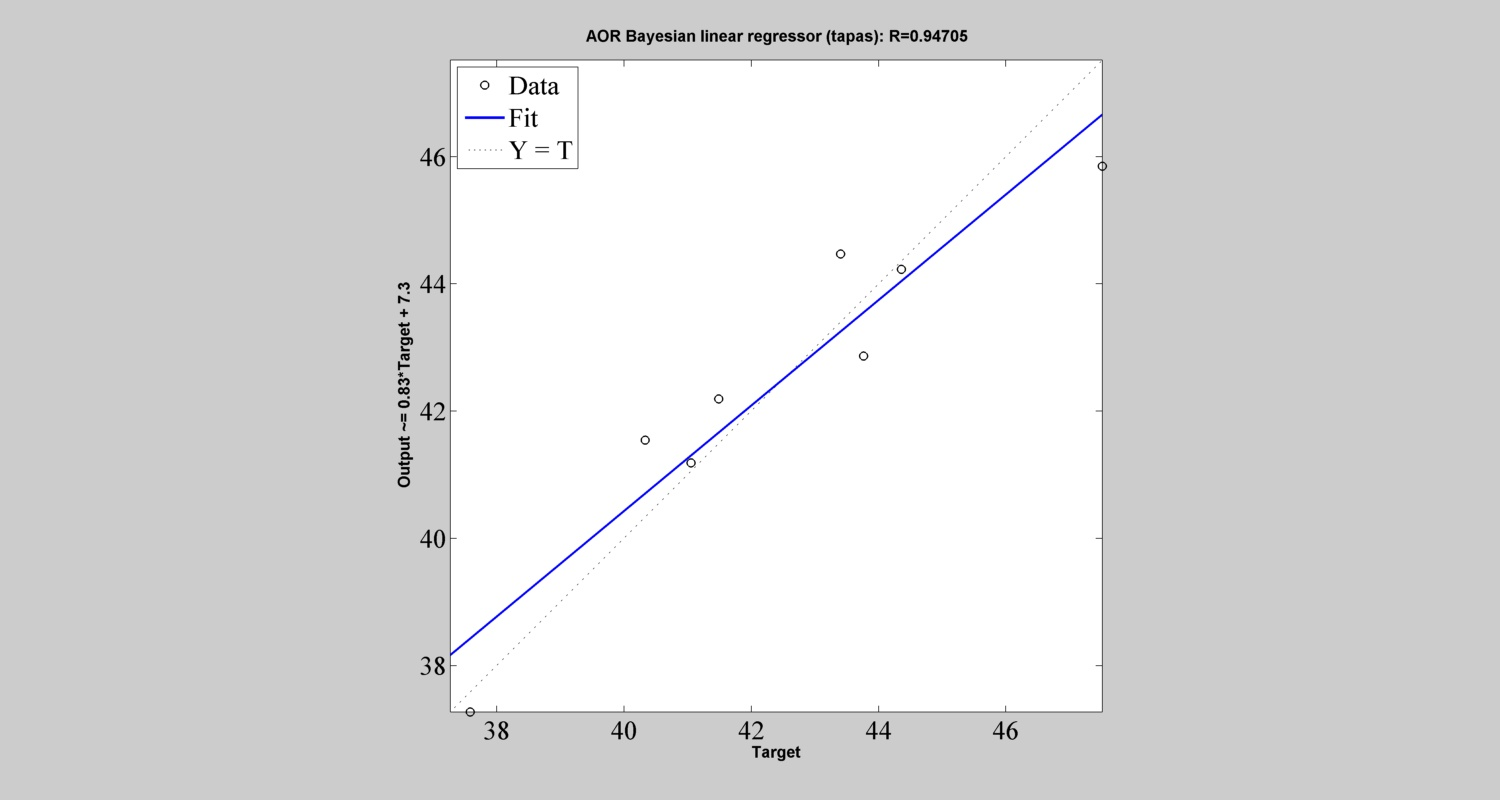
\includegraphics[width=.48\columnwidth]{images/072aorbayesianlinearregression}
	  \label{fig:072aorbayesianlinearregression}  }
  \\
    \subfloat[AoR Gaussian non linear regressor.]{
	  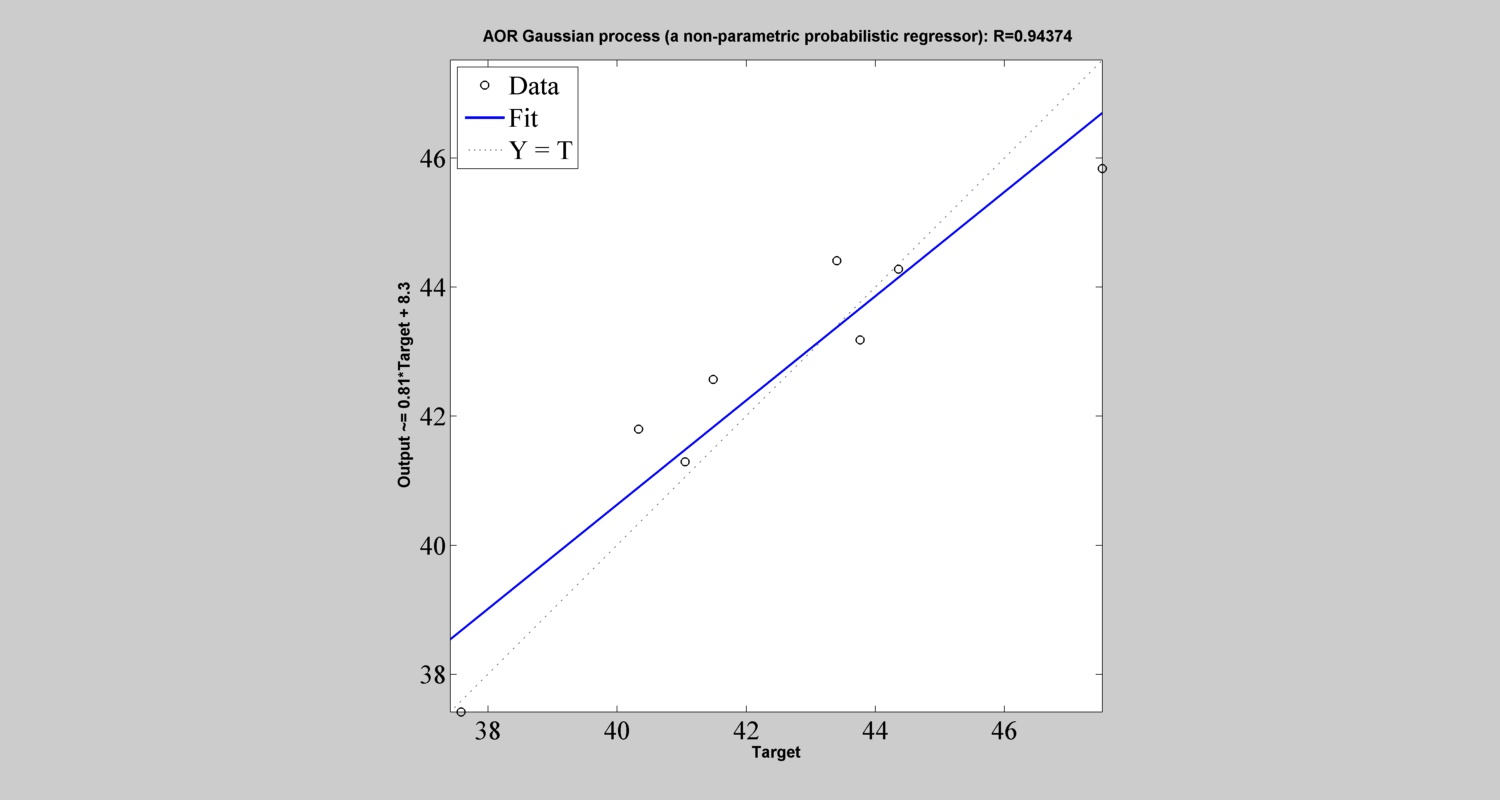
\includegraphics[width=.48\columnwidth]{images/073aorgaussiannonlinearregression}
	  \label{fig:073aorgaussiannonlinearregression}
  }
  \quad
 % \hfill
  \subfloat[AoR ANN non linear regression.]{
	  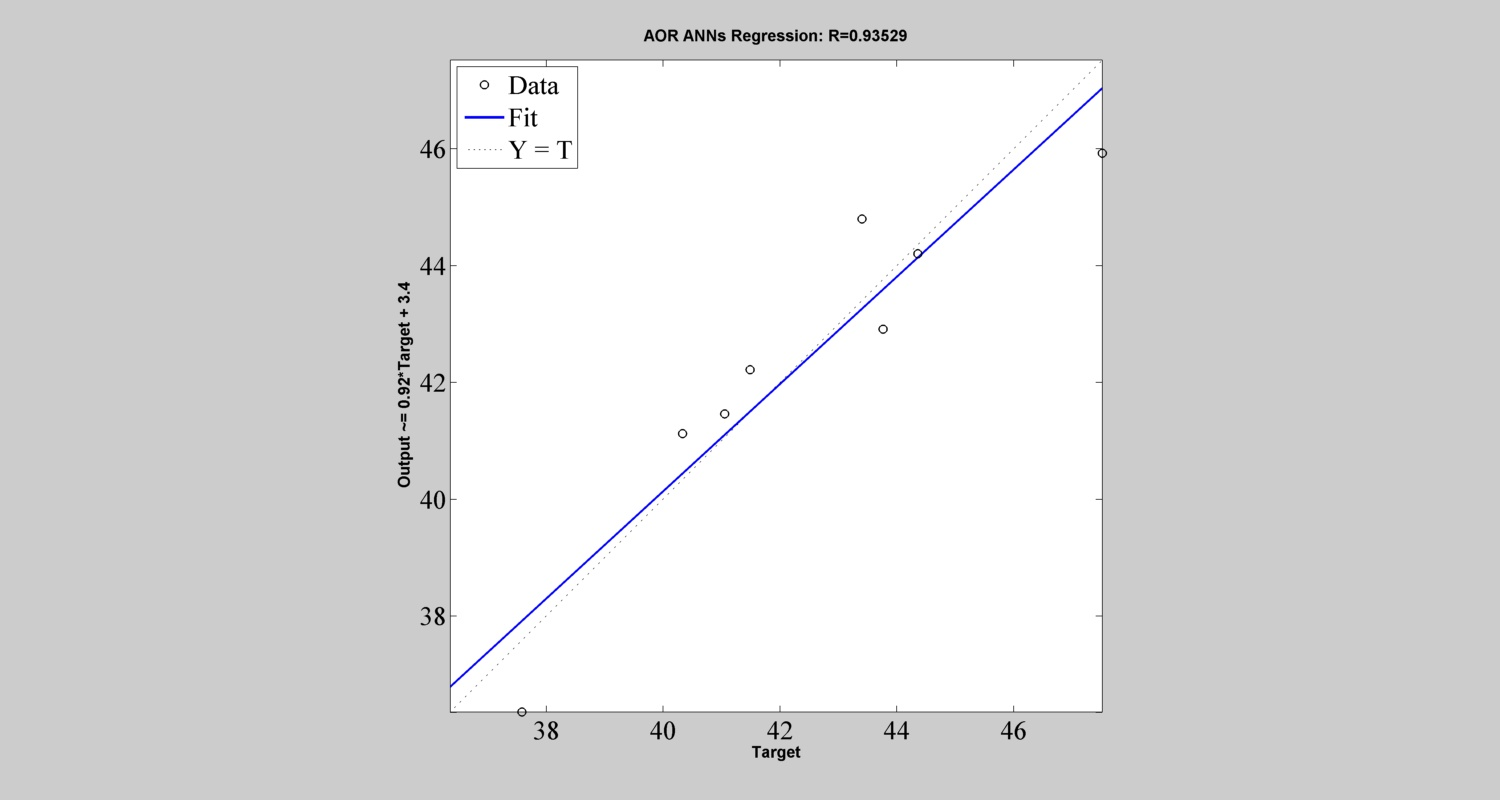
\includegraphics[width=.48\columnwidth]{images/074aorannnonlinearegression}
	  \label{fig:074aorannnonlinearegression}
  }
 % \hfill\null
  \caption{Regressions.}
  \label{fig:077regressions}
\end{figure}

% \begin{figure}%[!h] 
% \centering 
% 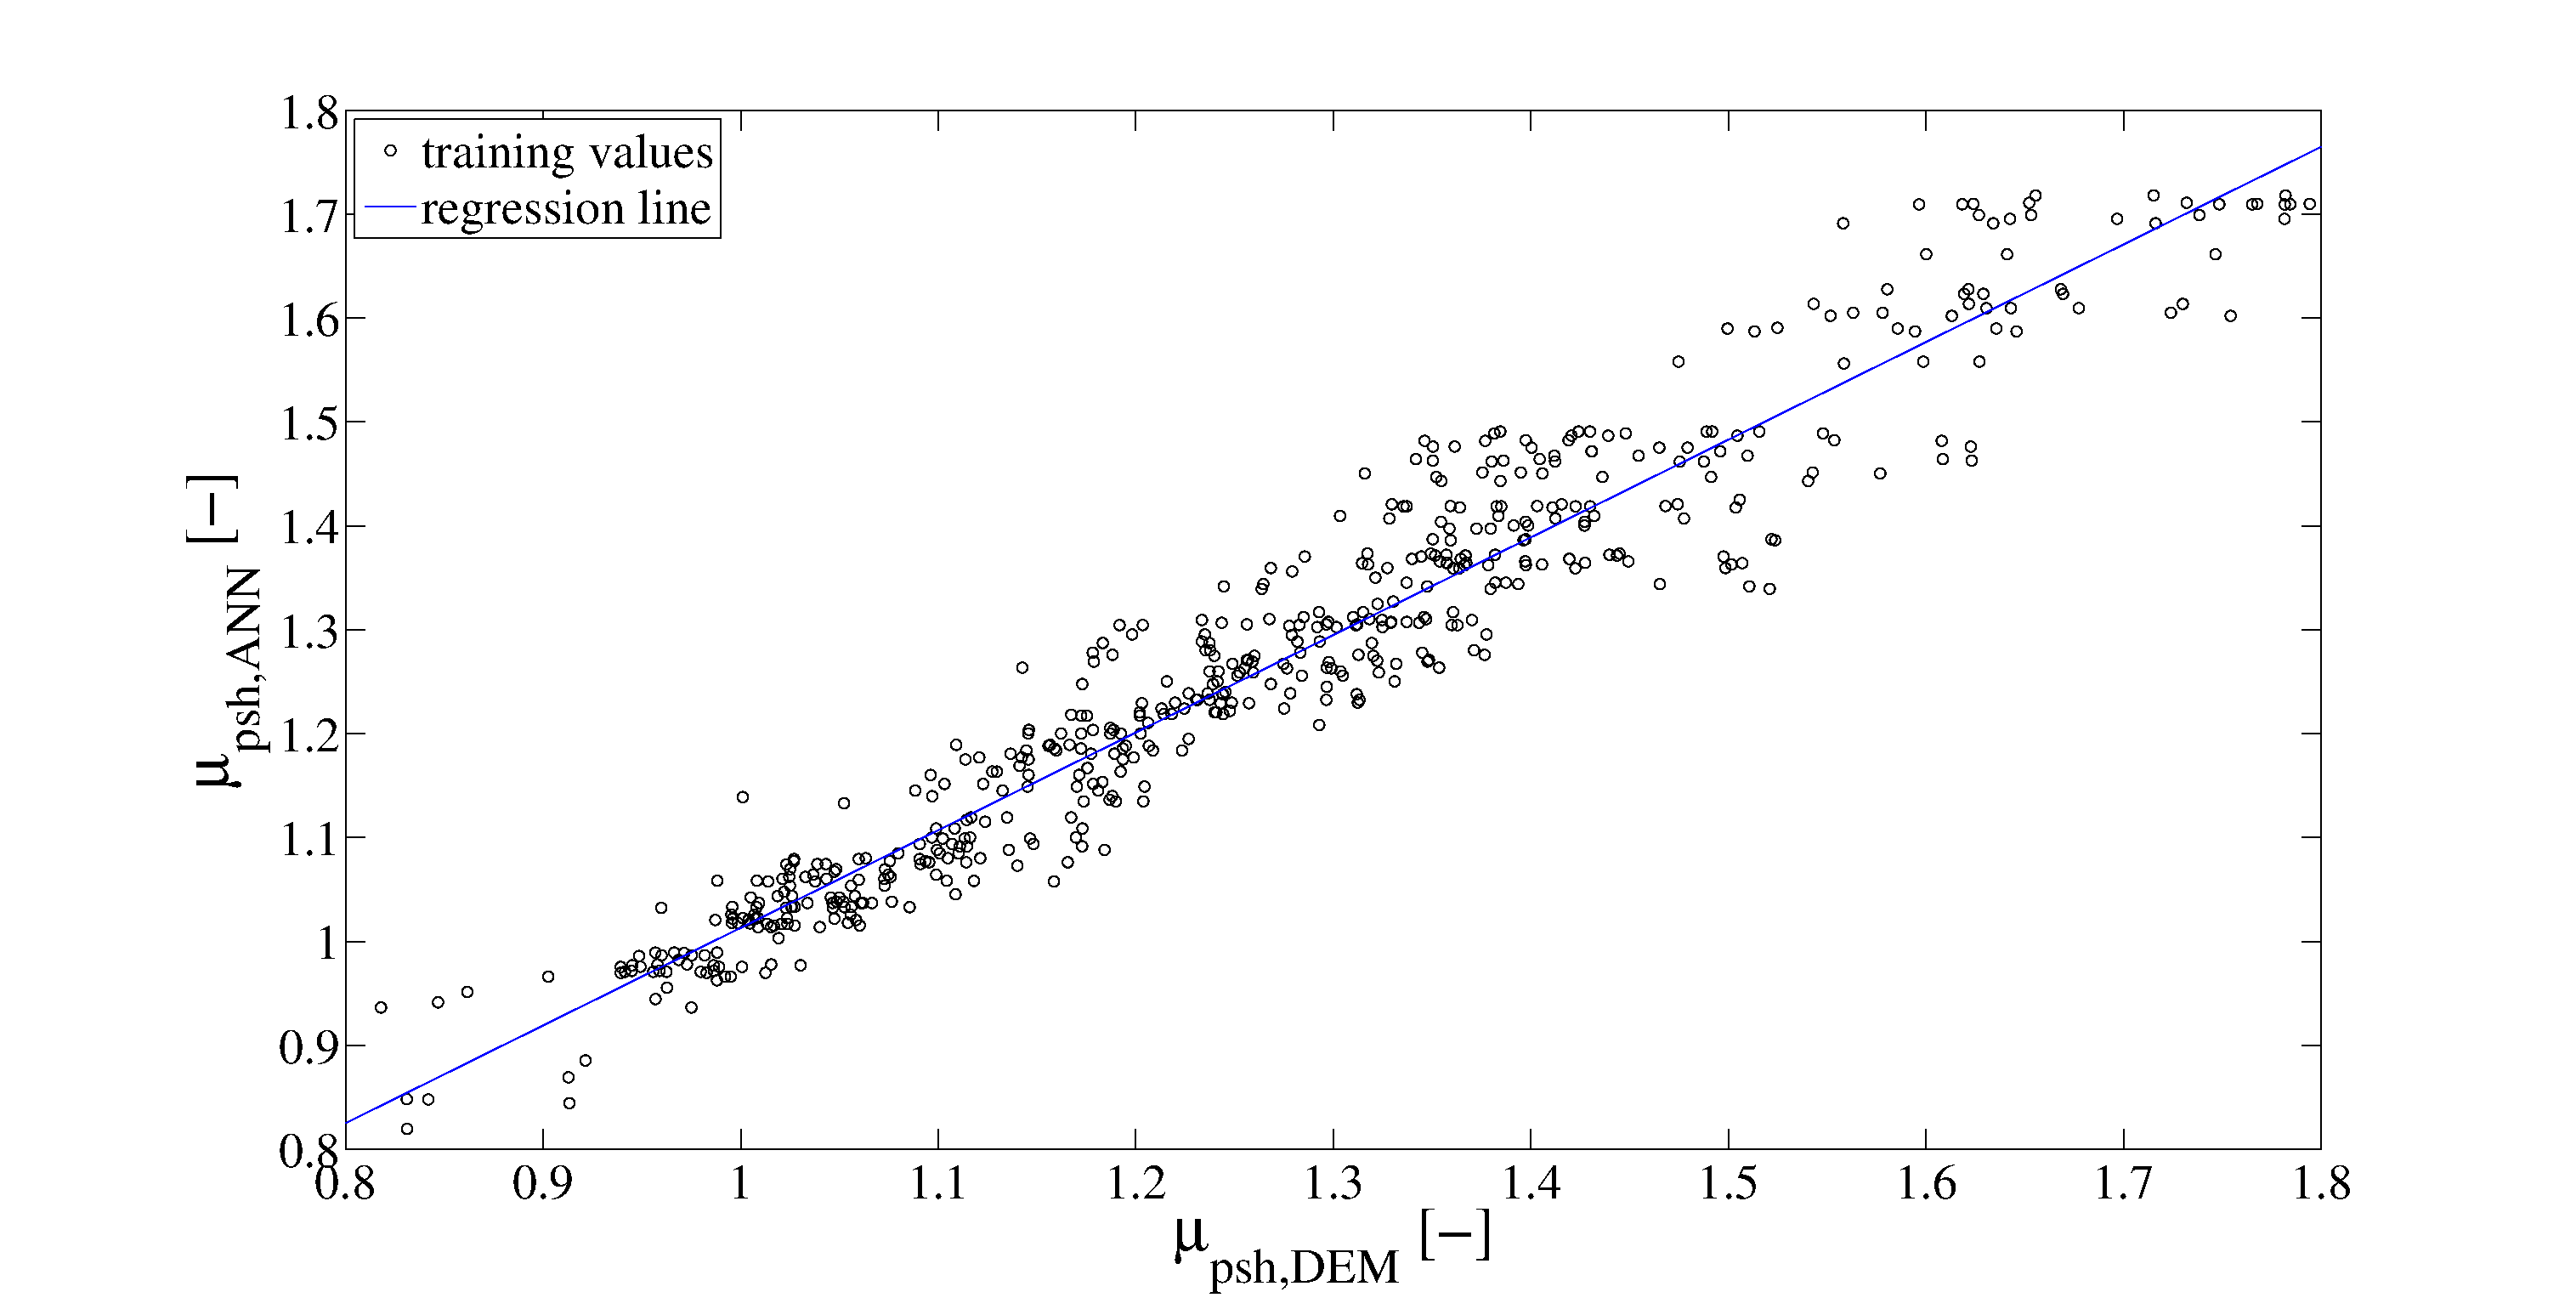
\includegraphics[width=.80\columnwidth]{images/022regression.eps}
% %[width=.48\textwidth]
% \caption[Comparison between prediction of the trained ANN and full DEM
% simulation]{Comparison between prediction of the trained Artificial Neural
% Network ($ANN$) and 546 
% \wrong{write down all the simulations performed at the end.}
% full DEM simulations of the coefficient of pre-shear
% (\ac{mupsh}).}
% \label{fig:022regression} 
% \end{figure}
\begin{figure}[htbp]
	\centering
  %\null\hfill
  \subfloat[SCT Bayesian linear regressor.]{
	  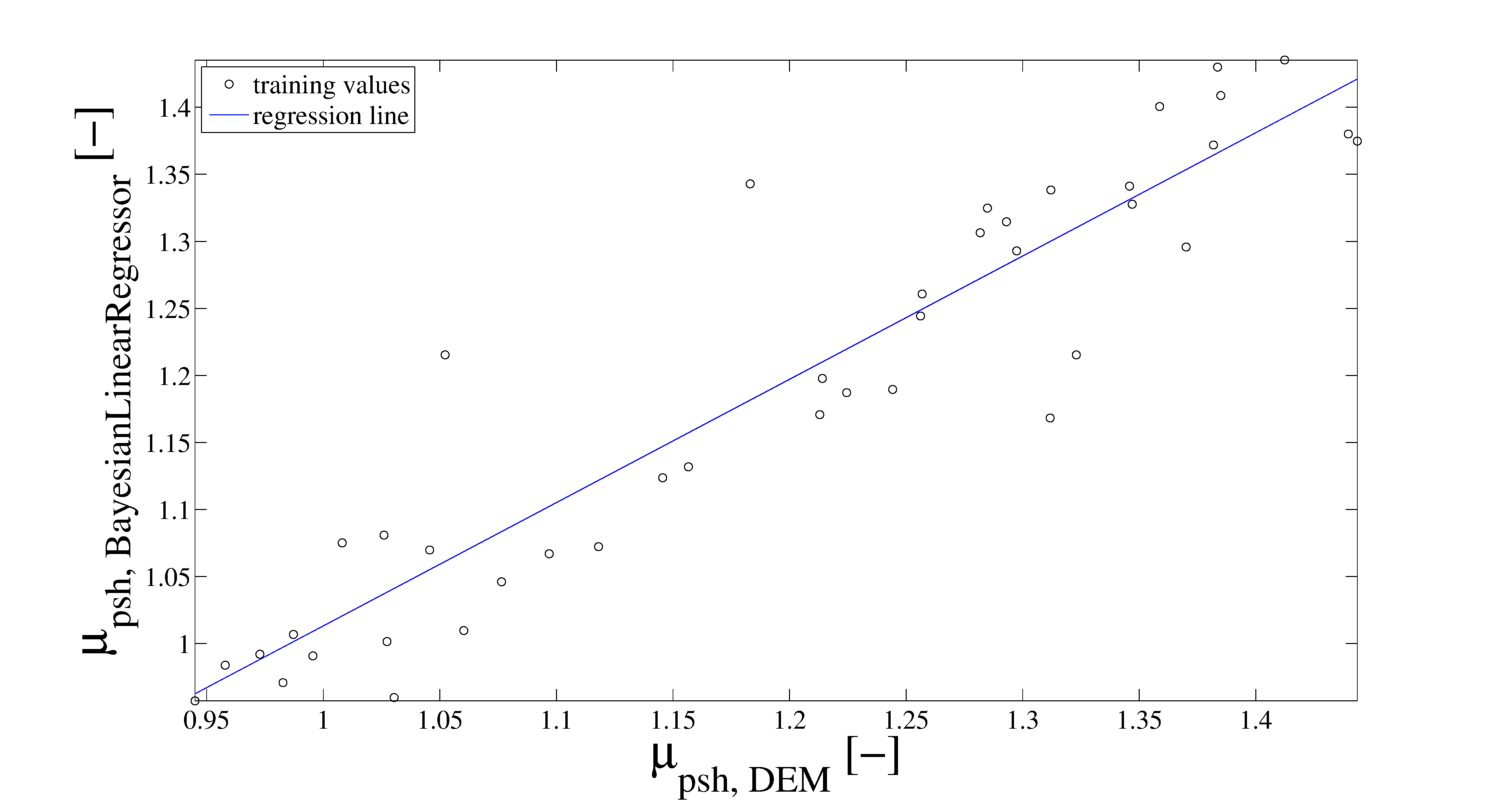
\includegraphics[width=.75\columnwidth]{images/137SCTBayesianLinearRegressor}
	  \label{fig:137SCTBayesianLinearRegressor}
  }
  \\
    \subfloat[SCT Gaussian non linear regressor.]{
	  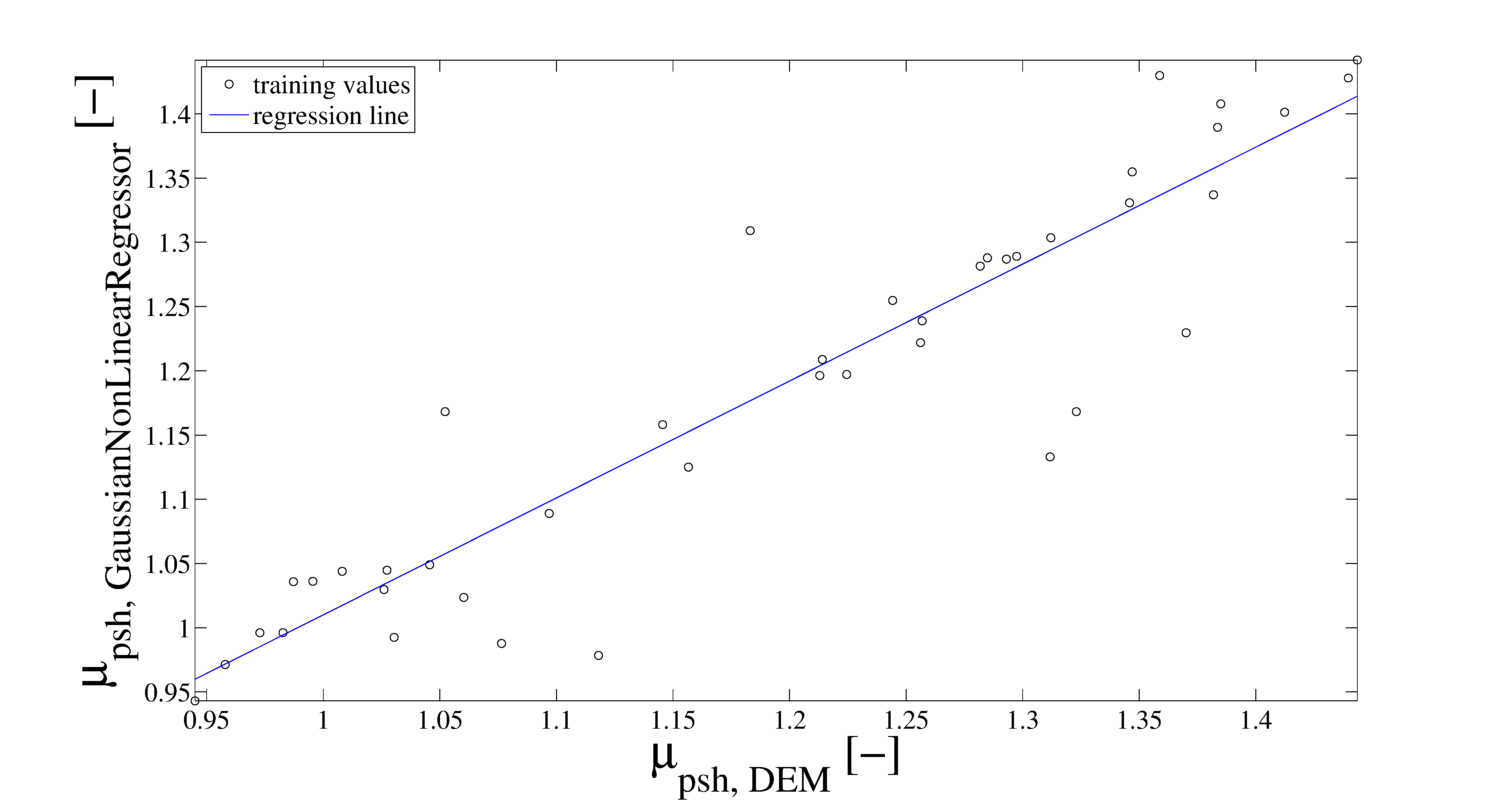
\includegraphics[width=.75\columnwidth]{images/138SCTGaussianNonLinearRegressor}
	  \label{fig:138SCTGaussianNonLinearRegressor}
  }
  \\
 % \hfill
  \subfloat[SCT ANN non linear regression.]{
	  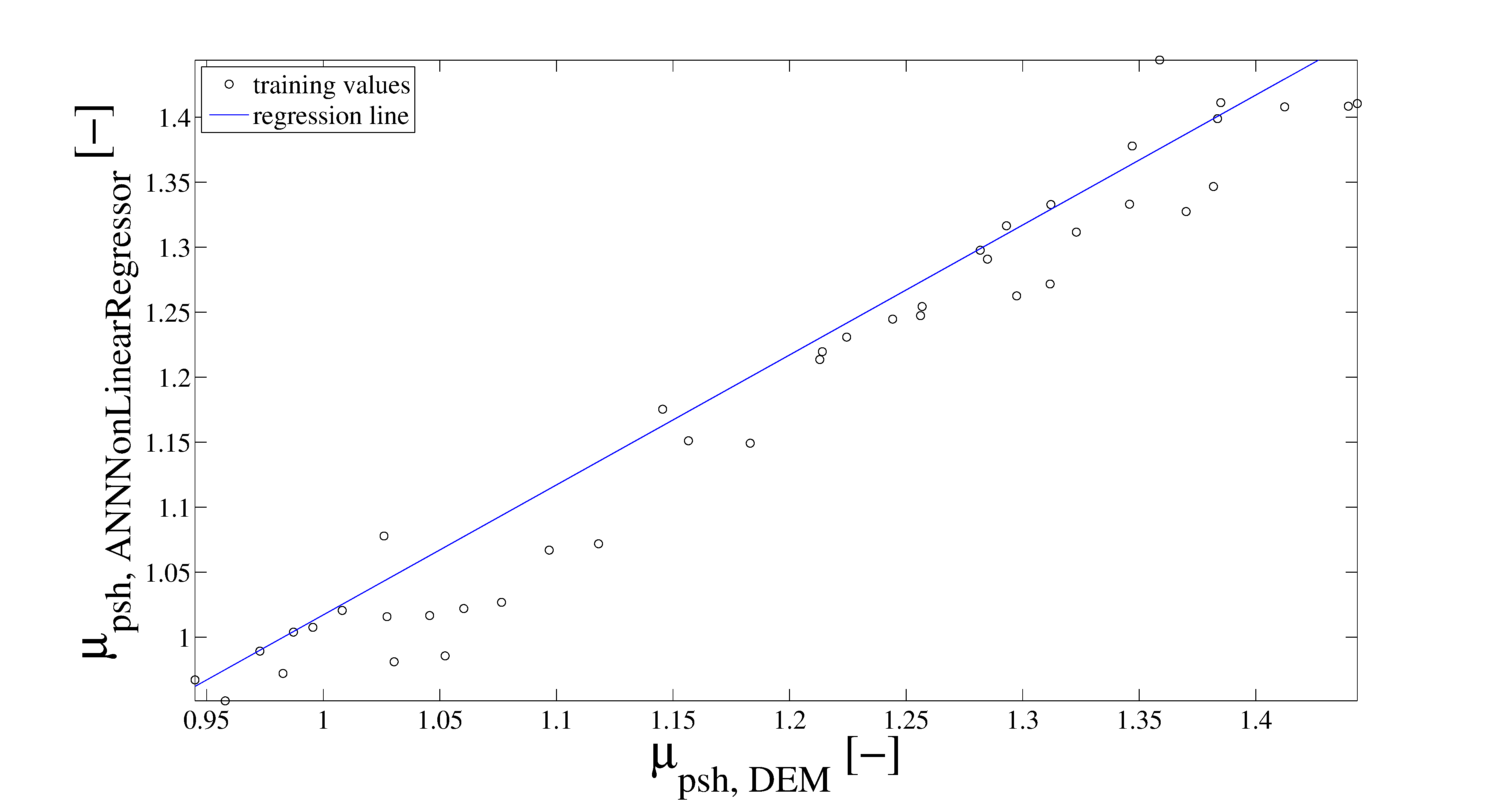
\includegraphics[width=.75\columnwidth]{images/139SCTANNNonLinearRegressor}
	  \label{fig:139SCTANNNonLinearRegressor}
  }
  \caption{Regressions comparison for the \acs{mupsh}.}
  \label{fig:143sctregressions}
\end{figure}

% \begin{figure}%[!h] 
% \centering 
% 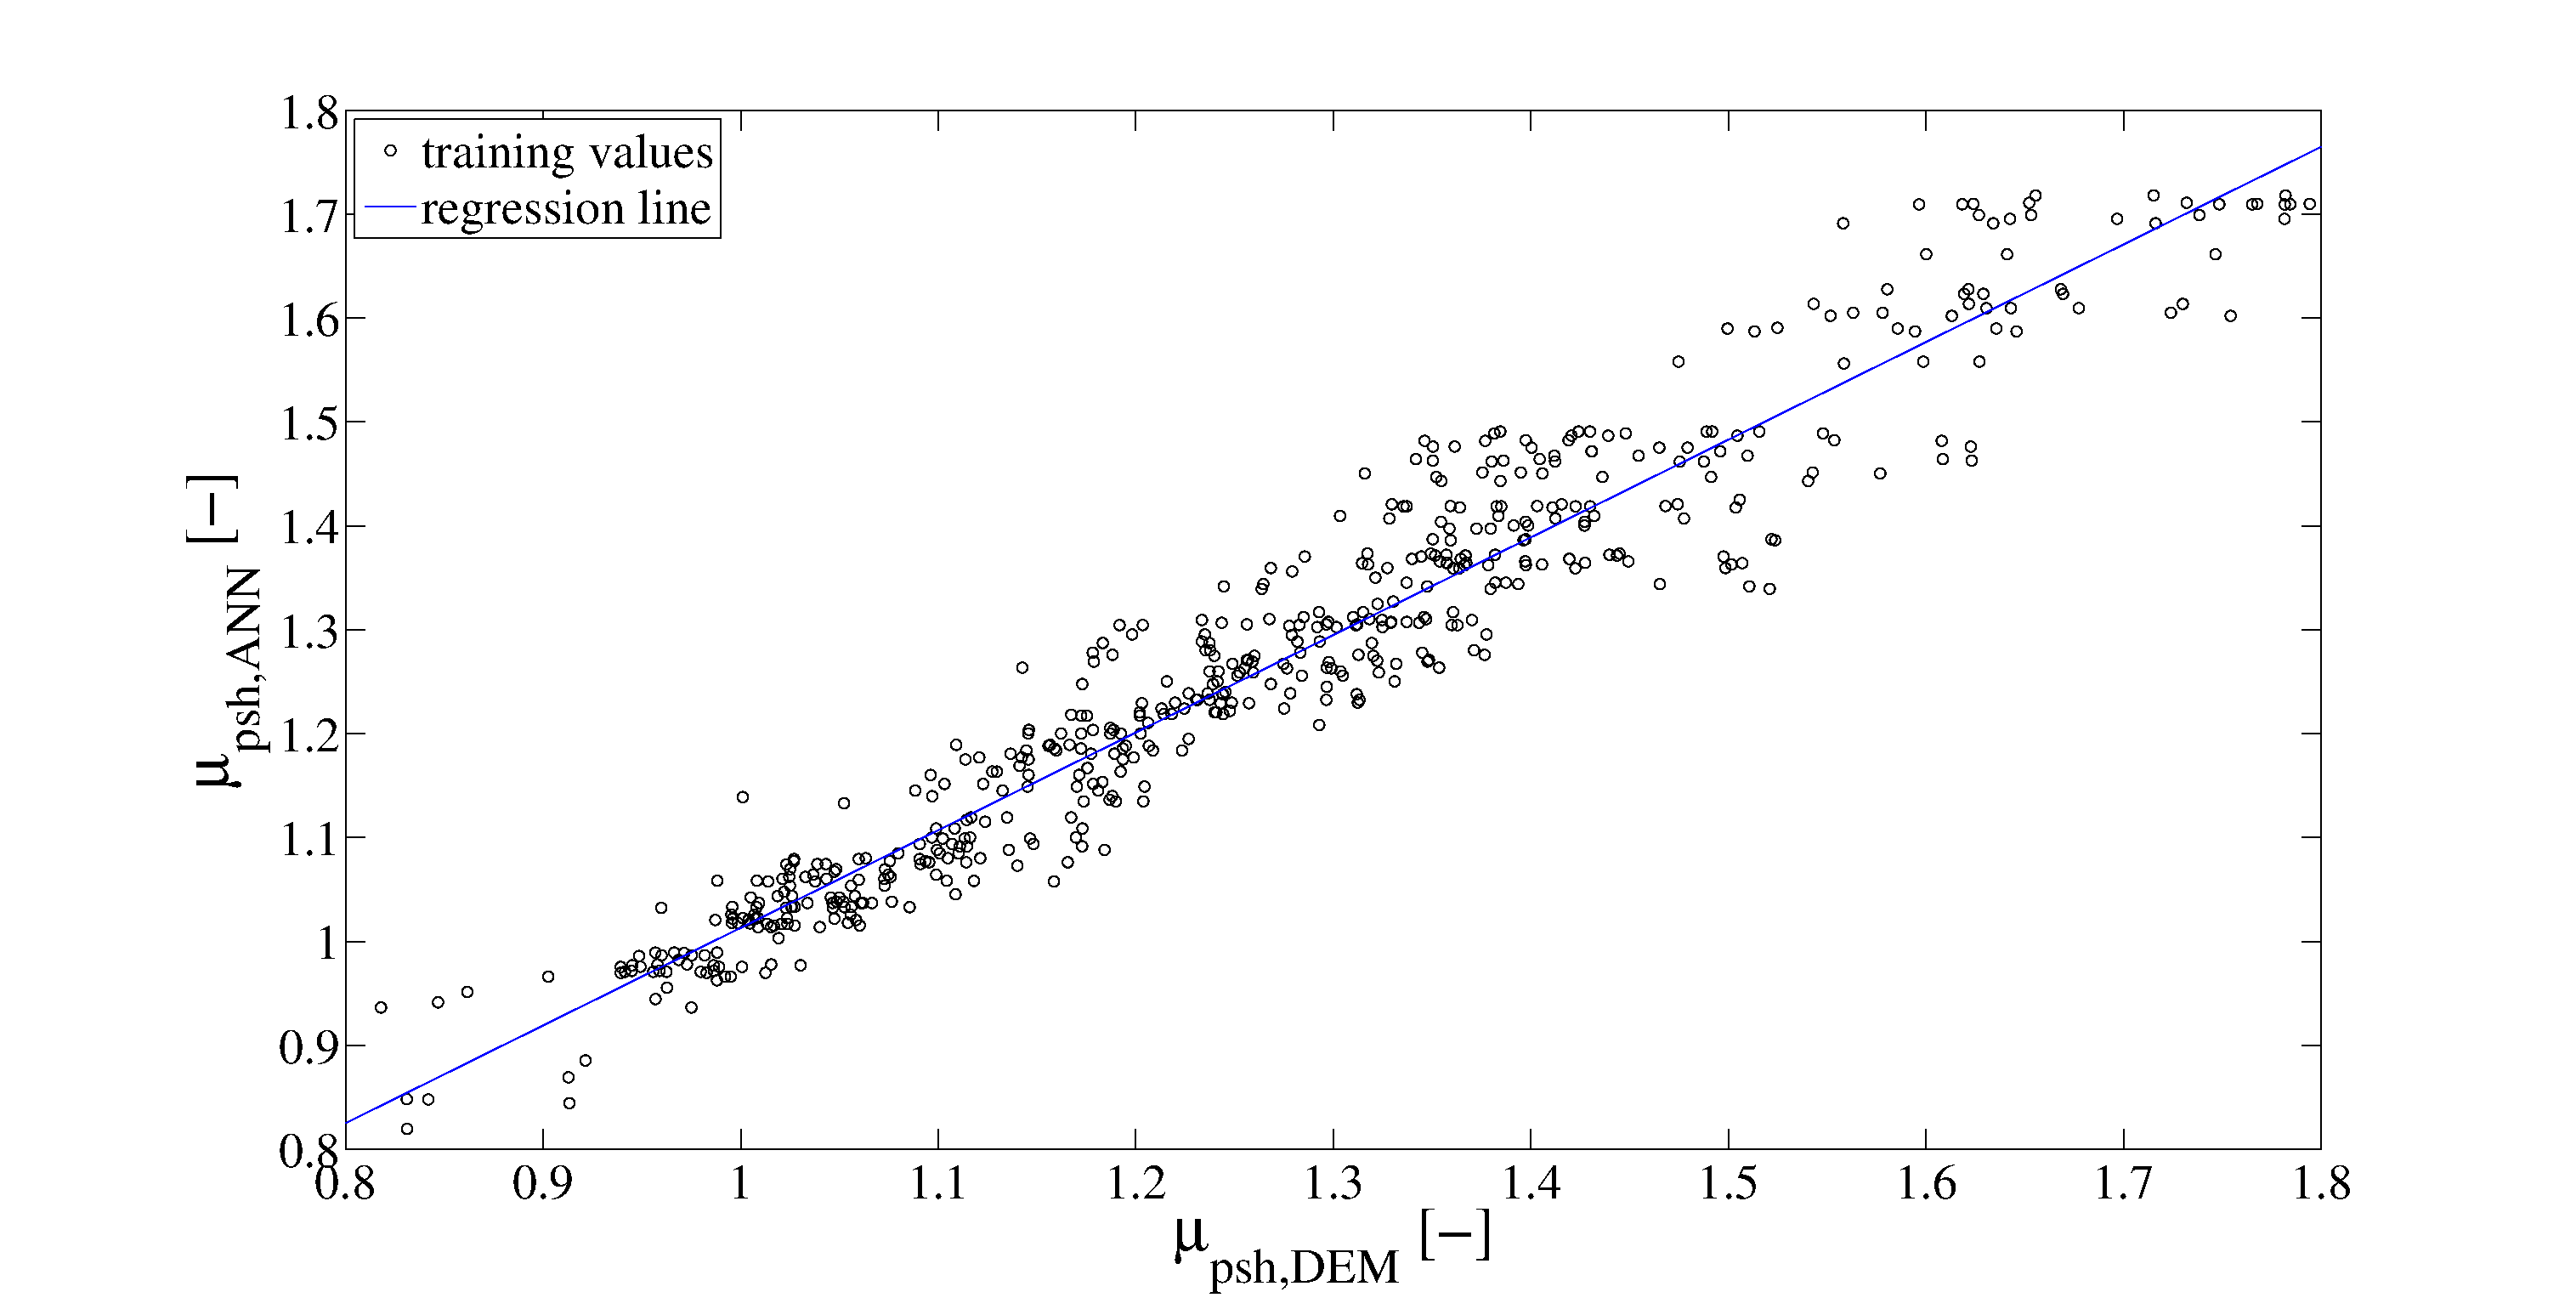
\includegraphics[width=.80\columnwidth]{images/022regression.eps}
% %[width=.48\textwidth]
% \caption[Comparison between prediction of the trained ANN and full DEM
% simulation]{Comparison between prediction of the trained Artificial Neural
% Network (\acs{ANN}) and 546 
% \wrong{write down all the simulations performed at the end.}
% full DEM simulations of the coefficient of pre-shear
% (\acs{mupsh}).}
% \label{fig:022regression} 
% \end{figure}
\begin{figure}[htbp]
	\centering

	 % \resizebox{12cm}{!}{\input{images/137SCTBayesianLinearRegressor.tikz}}


    \subfloat[AoR Bayesian linear regressor.]{
	  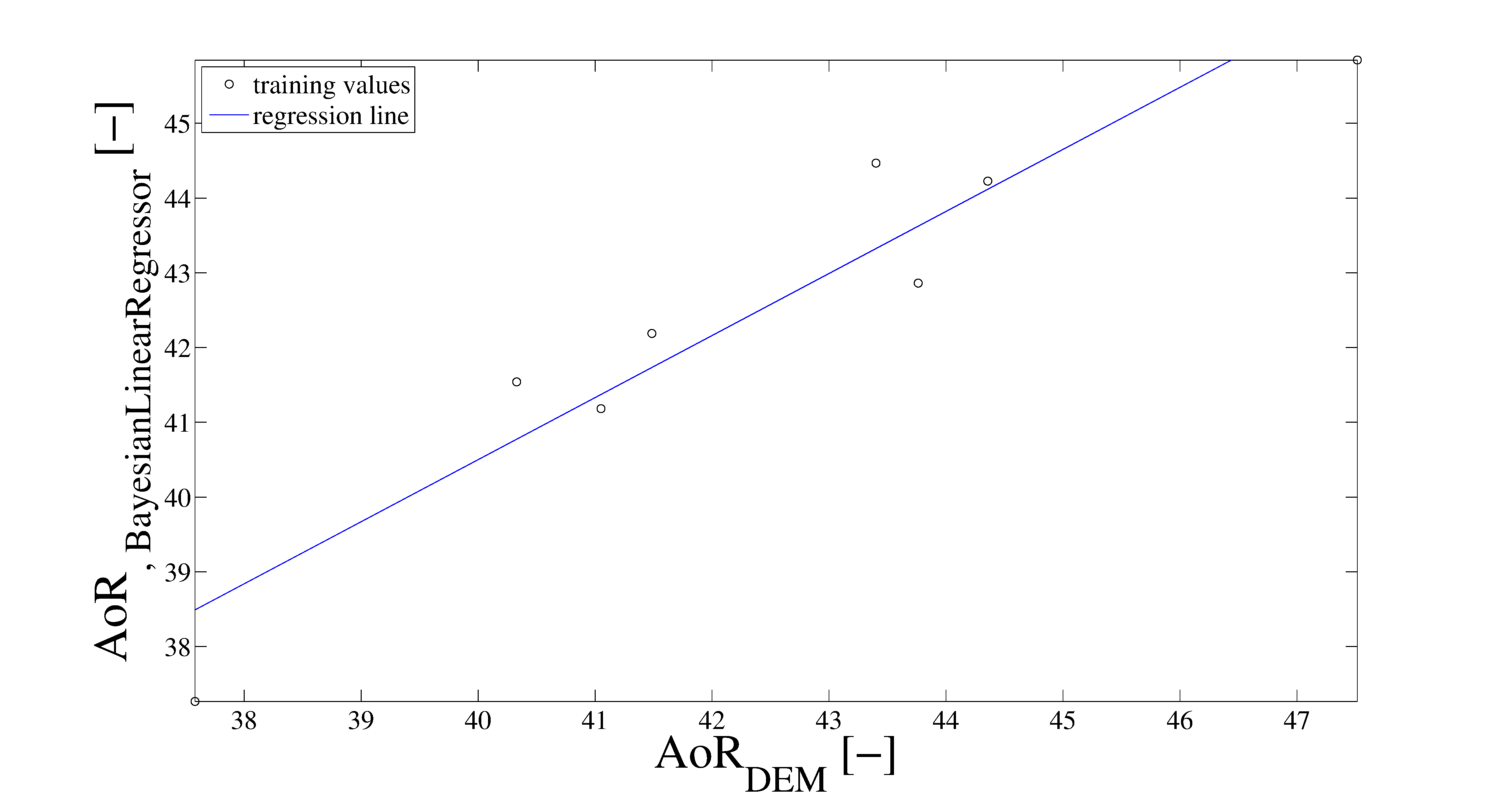
\includegraphics[width=.75\columnwidth]{images/140AoRBayesianLinearRegressor}
	  \label{fig:140AoRBayesianLinearRegressor}  }
  \\
    \subfloat[AoR Gaussian non linear regressor.]{
	  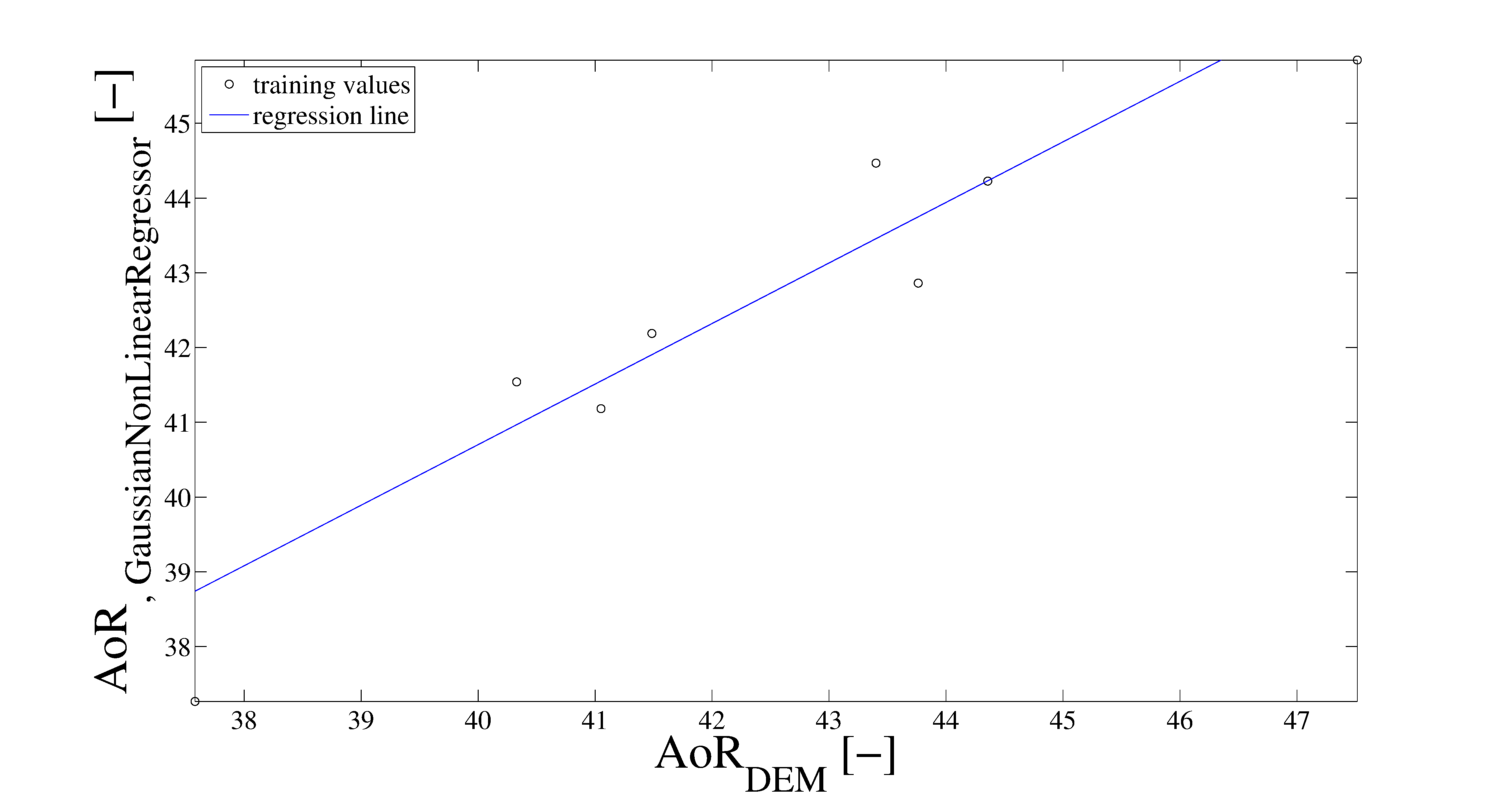
\includegraphics[width=.75\columnwidth]{images/141AoRGaussianNonLinearRegressor}
	  \label{fig:141AoRGaussianNonLinearRegressor}
  }
  \\
 % \hfill
  \subfloat[AoR ANN non linear regression.]{
	  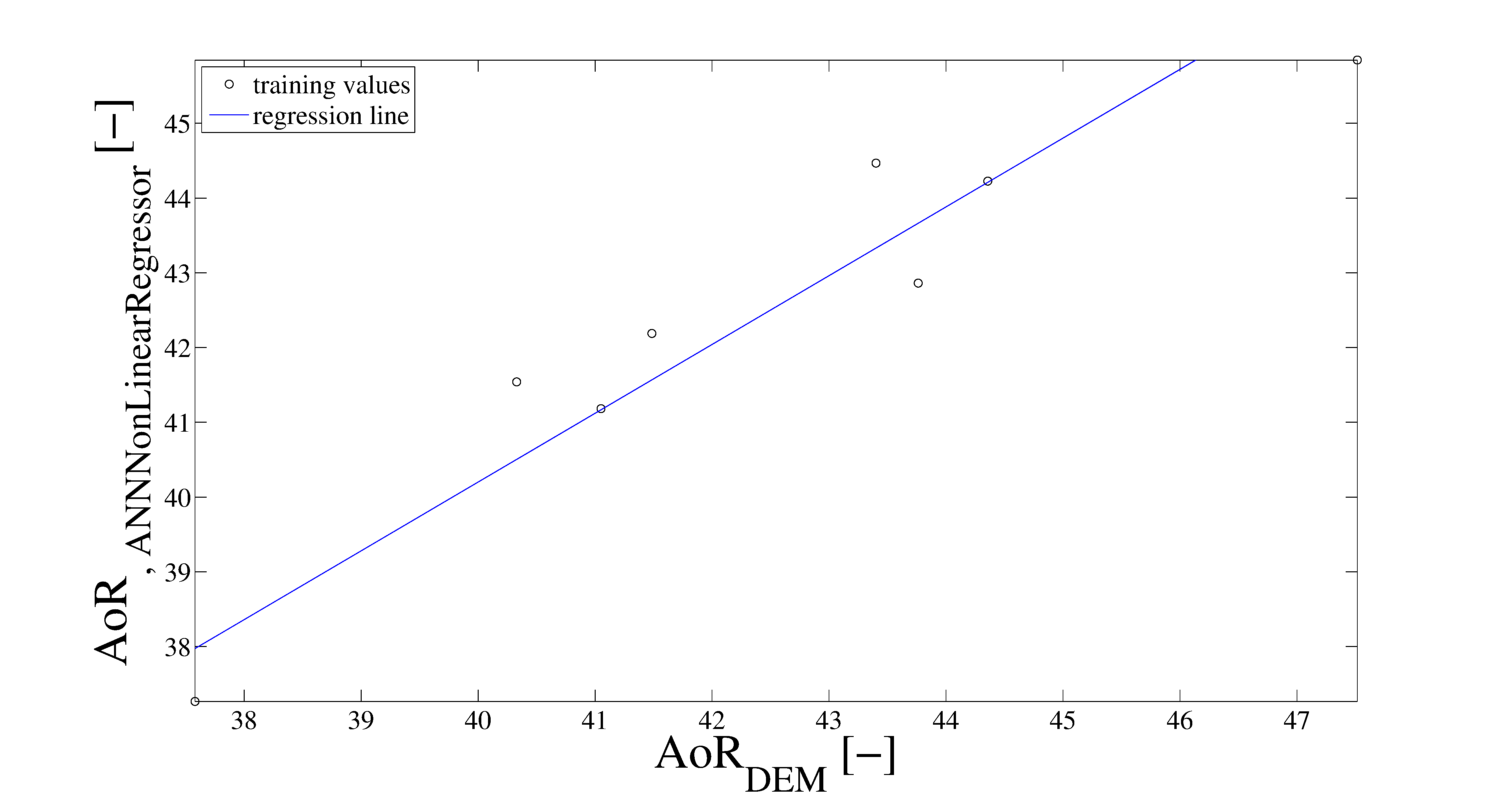
\includegraphics[width=.75\columnwidth]{images/142AoRANNNonLinearRegressor}
	  \label{fig:142AoRANNNonLinearRegressor}
  }
 % \hfill\null
  \caption{Regressions comparison for the \acs{AoR}.}
  \label{fig:144aorregressions}
\end{figure}

% \begin{figure}%[!h] 
% \centering 
% 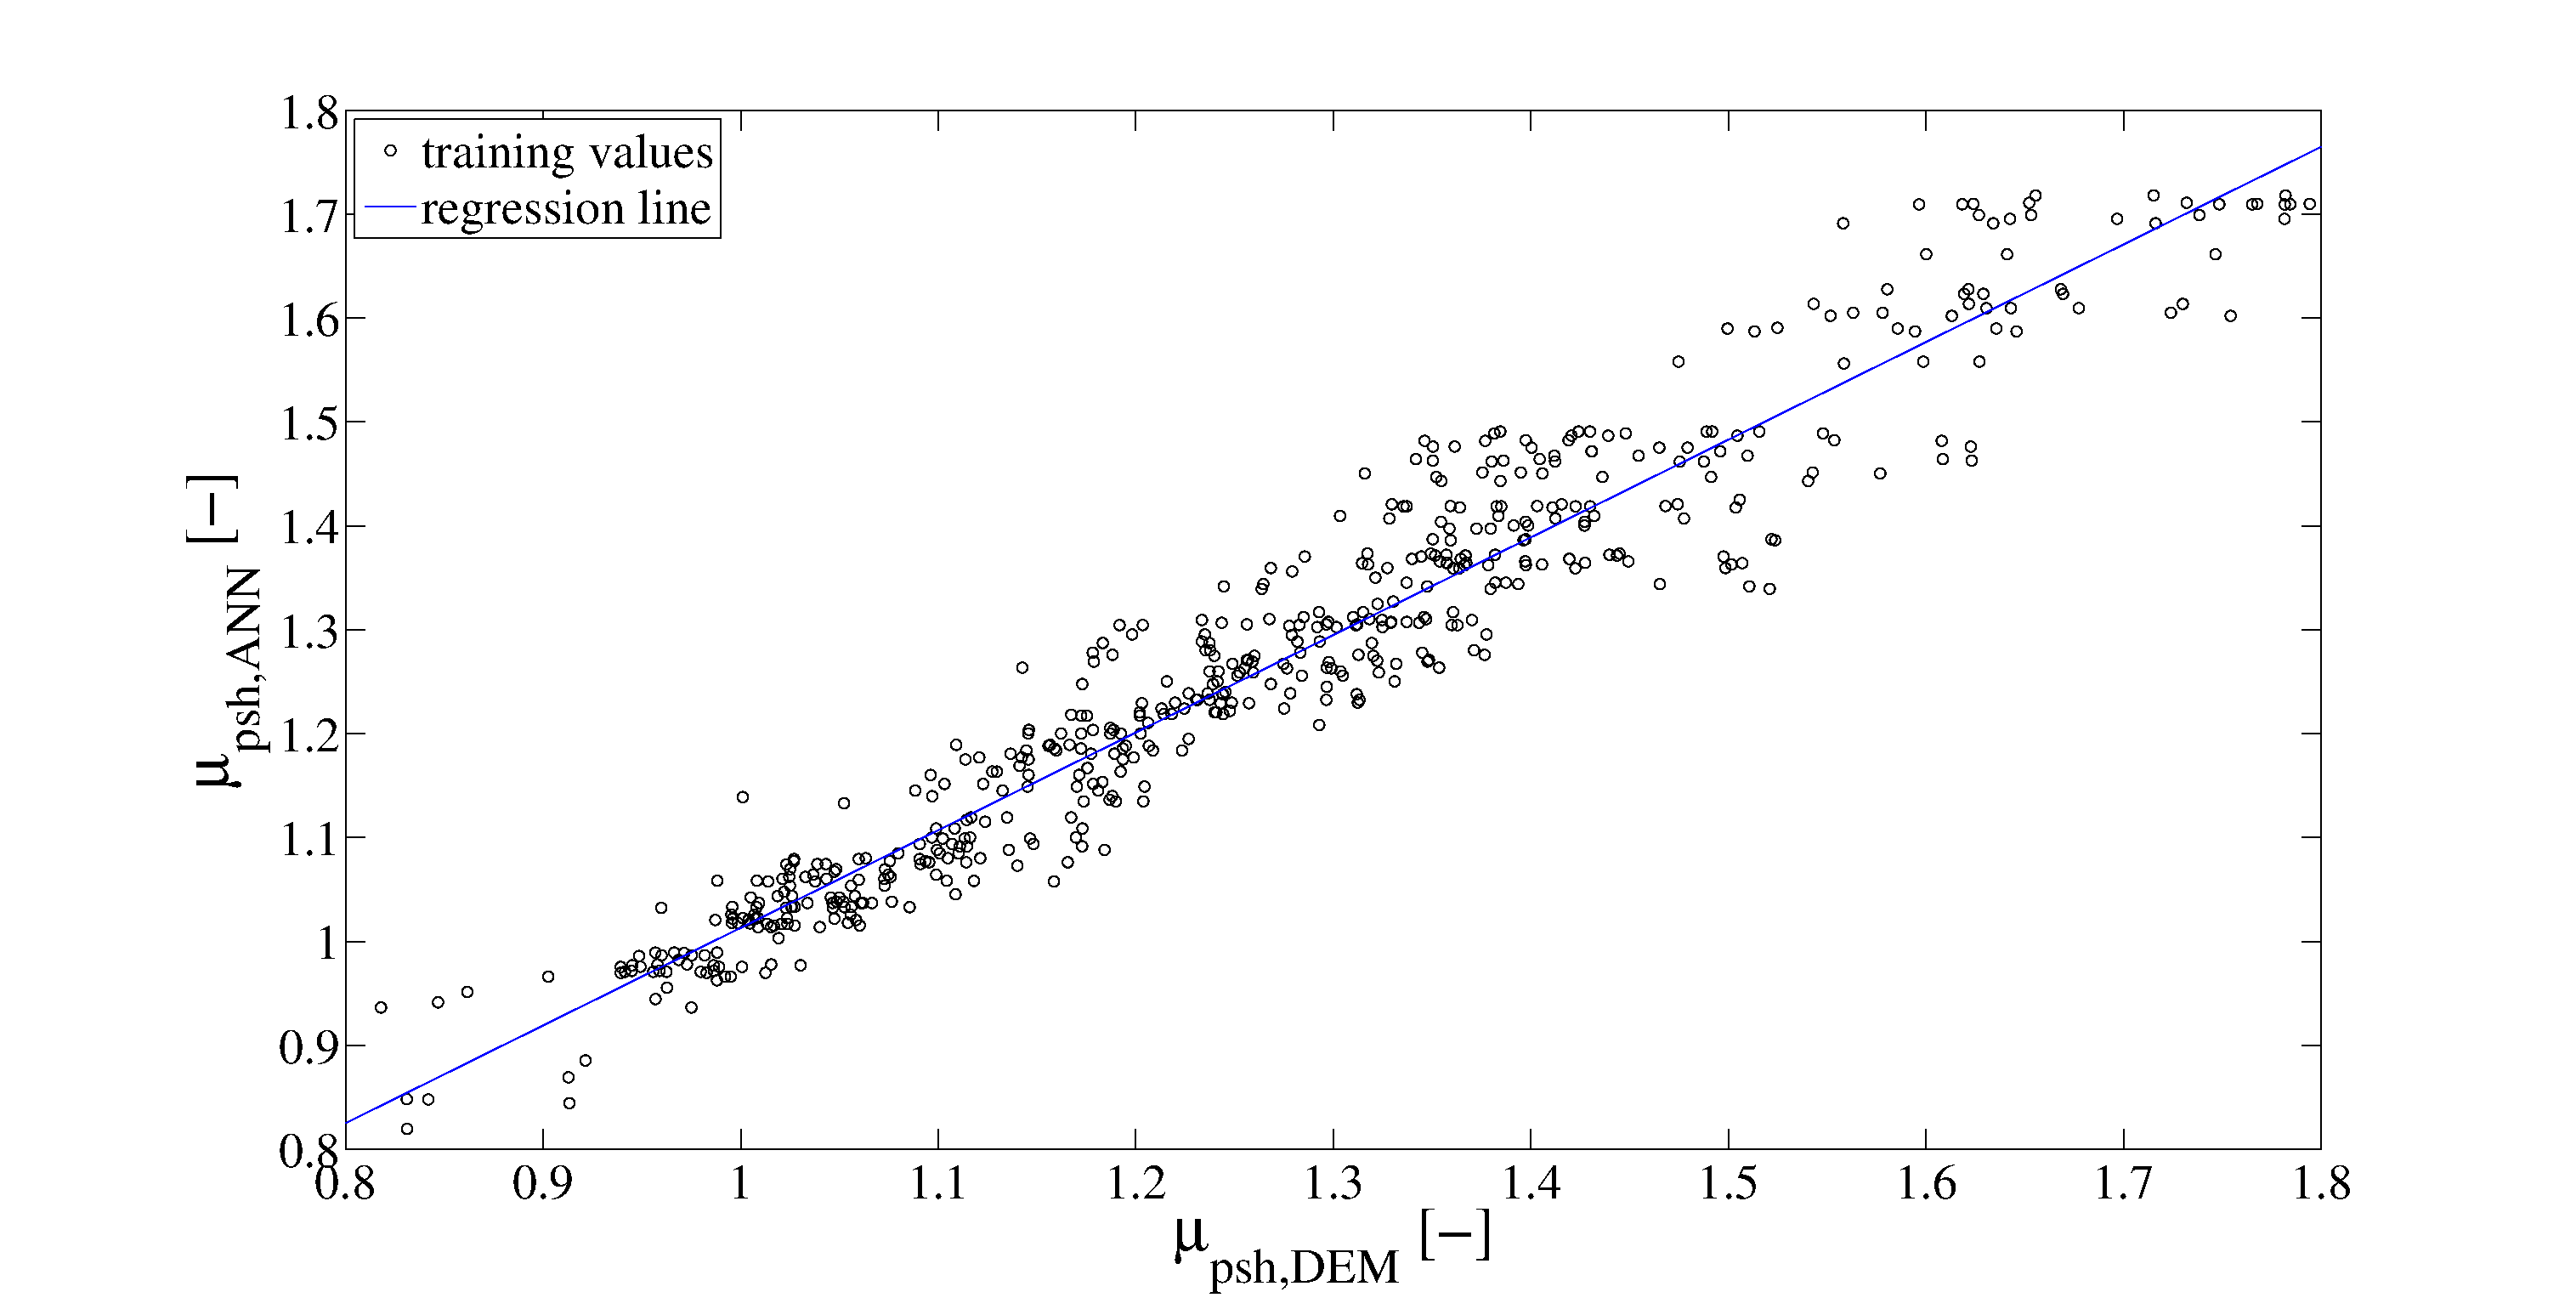
\includegraphics[width=.80\columnwidth]{images/022regression.eps}
% %[width=.48\textwidth]
% \caption[Comparison between prediction of the trained ANN and full DEM
% simulation]{Comparison between prediction of the trained Artificial Neural
% Network (\acs{ANN}) and 546 
% \wrong{write down all the simulations performed at the end.}
% full DEM simulations of the coefficient of pre-shear
% (\acs{mupsh}).}
% \label{fig:022regression} 
% \end{figure}

We checked \acs{r2}, \textit{mean absolute error}, 
\begin{equation}
MAE = \frac{\sum _{i=1}^{n} (x_{i}-\widehat{x}_{i})}{n} ,
\label{eq:meanAbsoluteError}
\end{equation}
\textit{mean squared error},
\begin{equation}
MSE = \frac{\sum _{i=1}^{n} (x_{i}-\widehat{x}_{i})^{2}}{n}
\label{eq:meanSquareError}
\end{equation}
and \textit{root mean squared error},
\begin{equation}
RMSE = \sqrt{\frac{\sum _{i=1}^{n} (x_{i}-\widehat{x}_{i})^{2}}{n}}
\label{eq:rootMeanSquareError}
\end{equation}
for the \textit{Bayesian linear
regression}, the \textit{Gaussian nonlinear
regression}, and the
\textit{\acs{ANN} regression} to establish the most effective method.
All were trained with the same training set. 
For instance, a comparison of the \acs{r2} for the \acs{mupsh} can be see in 
Fig. \ref{fig:143sctregressions}.
In Fig. \ref{fig:144aorregressions} a similar comparison for the \acs{AoR} can
be found.\\
In fact, the check was performed for each method by comparing the
\acs{DEM} bulk values of the test set against the bulk values predicted by each method from the 
corresponding \acs{DEM} input values of the test set. \\
Table \ref{tab:15regressionvalues} shows a quantitative comparison between the
three methods for the \acs{mupsh}. 
\begin{table}[htbp]
  \centering

    \begin{tabular}{lccc}
    \hline
          & Bayesian & Gaussian & ANN \\
          \hline
    Coefficient of determination (\acs{r2}) & 0.86  & 0.843 & 0.959 \\
    Root mean squared error & 0.057 & 0.061 & 0.031 \\
    Mean absolute error & 0.042 & 0.038 & 0.025 \\
    Mean squared error & 0.003 & 0.004 & 0.001 \\
    \hline
    \end{tabular}%
      \caption{Regression methods quantitative comparison.}
  \label{tab:15regressionvalues}%
\end{table}%
%************************************************

\section{Parameter Identification}
\label{sec:parameteridentification}

Since \acs{mupsh}, \acs{mush} and \acs{rhob} belonged to the shear-cell
simulations, their \acs{ANNs} were handled together: we had one cluster with three 
\acs{ANNs} for the shear cell and one with only one \acs{ANN} for the \acs{AoR}.
We could then proceed in identifying valid input parameters.

\subsection{Computational Condiderations}
\label{subsec:computationalcondiderations}

\citet{RefWorks:116, RefWorks:160} suggested using a Design of Experiments
(\acs{DoE}) method to determine the parameter combinations to be simulated.
They stated that this approach allows optimization of computation time
with an acceptable loss of precision.
The speed of the trained \acs{ANNs} enabled us to follow a different approach to
maximizing the precision of the characterization.\\

\begin{table}[h]
\centering
\begin{tabular}{lcccc}
\hline
 &  \ac{mus} & \ac{mur} & \ac{CoR} & \ac{rhop}  \\
  &	$[-]$  & $[-]$   & $[-]$   & $[kg/m3]$ \\
          \hline
    range & $[0.1 \ldots 1.0]$ & $[0.1 \ldots 1.0]$ & $[0.5 \ldots 0.9]$ &
    $[2000 \ldots 3500]$     \\
    \# rnd & 100   & 100   & 25    & 25    \\

\hline
\end{tabular}
\caption[DEM random input values]{DEM random input values. Within each range \#
random values are chosen.}
\label{tab:12DEMRandominputvalues}
\end{table}

\subsection{Decisional Limits}
\label{subsec:decisionallimits}

We created random values
in the range and numbers defined in Table \ref{tab:12DEMRandominputvalues}
according to a standard uniform distribution.
These combinations were then fed to and processed by the selected
\acs{ANNs}, and thus three bulk values for the shear
cell and one for the \acs{AoR} were obtained.
The \acs{ANN} evaluation was significantly faster than the \acs{DEM} simulations. The
individuation of the numerical bulk behaviours for all the \acs{DEM} combinations
did not take more than a few seconds on a single core.\\
\begin{figure}[!htb] 
\centering 
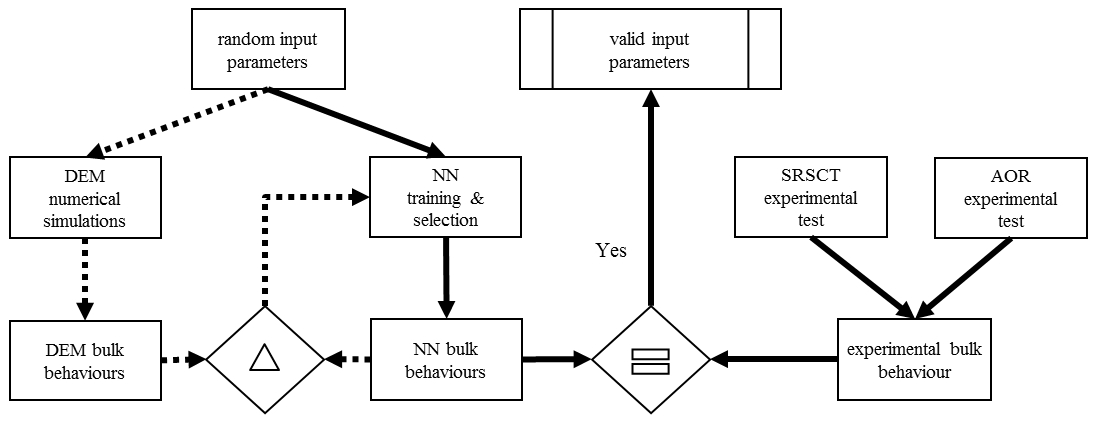
\includegraphics[width=.96\textwidth]{images/019methodology} 
\caption[Method]{Method. In the training phase (dashed lines)
$DEM$ simulations are performed
with random initial input parameters.
The behaviours obtained are used to train the
Artificial Neural Networks ($ANNs$) in a loop that continues until the
difference between the outputs of each $ANN$ and its simulations is below the
limit ($\Delta$).
In the parameters identification phase (solid
lines) we identify valid input parameters by comparing (\textbf{=}) $ANNs$ and
experimental behaviours.}
\label{fig:019methodology} 
\end{figure}
As can be seen in Fig. \ref{fig:019methodology}, in the parameters
identification phase (solid lines) we identify valid input parameters by comparing (\textbf{=}) \acs{ANNs} and
experimental behaviours.\\
We obtained for each of the twelve load conditions of the \acs{SCT} three bulk
values (\acs{mupsh}, \acs{mush} and \acs{rhob}).
The fourth bulk value was the result of two angle of repose (\acs{AoR}) tests that
recreated the repose angle observed in a pile of the
real material. 
Subsequently, we compared the \acs{ANN} and experimental bulk behaviours for the
twelve shear-cell load conditions.
If in a DEM-parameter combination all the three bulk values differed by less 
than 5\% from those of the corresponding experiments, i.e.:
%************************************************
\begin{equation}
 \begin{cases}
\text{if } & \lvert{1-\frac{\mu_{psh,num}}{\mu_{psh,exp}}}\rvert < 5\%  ,\\
\text{and if } & \lvert{1-\frac{\mu_{sh,num}}{\mu_{sh,exp}}}\rvert < 5\% , \\ 
\text{and if } & \lvert{1-\frac{\rho_{p,num}}{\rho_{p,exp}}}\rvert < 5\% ,\\ 
\end{cases}
 \label{eq:check2}
\end{equation}
the combination was marked. The marked combinations were processed by the
\acs{AoR} \acs{ANN}, and then compared with the experiment.
Were considered valid those that differed by less than $5\%$ also in this
comparison (Eq. \ref{eq:checkaor}):
%************************************************
\begin{equation}
\text{if} ~~~~~~ \lvert{1-\frac{AoR_{num}}{AoR_{exp}}}\rvert < 5\% .
\label{eq:checkaor}
\end{equation}
%************************************************

\section{Sinter fine Characterization}
\label{sec:sinterfinecharacterization}

We realized 6,250,000 parameter of combinations random values for sinter fine.
Amongst them we searched for values complying with the experimental results.
Further, we investigated the reliability of the procedure, see Section
\ref{subsec:reliabilityconsiderations}.\\
The comparison between numerical and experimental behaviours led to a first
series of marked combinations ($MC1$) for two load conditions of
the shear cell:
\begin{itemize}
  \item{$\acs{sigman} = 1,068$ Pa, P=1.0, as plotted in Fig.
  \ref{fig:041radarpirker1schulze1068},}
  \item{$\acs{sigman} = 10,070$ Pa, P=1.0, as plotted in Fig.
  \ref{fig:024radarpirker1schulze10070}.}
\end{itemize}
We decided to show the valid values achieved through the procedure for every
material analyzed with three compact graphical schemes:

\begin{itemize}
  \item{parameter space plot,}
  \item{box plot,}
  \item{density plot.}
\end{itemize}

In the following sections, the plots regarding the sinter fine with
$\acs{sigman} = 10,070$ Pa are discussed and interpreted as pattern for each
material in each load condition.

\subsection{Parameter space plot}
\label{subsec:parameterspaceplot}

An example of a parameter space plot can be seen
in Fig. \ref{fig:024radarpirker1schulze10070}.
On the axes we can see:
\begin{itemize}
  \item{the \acl{CoR} (\acs{CoR}),}
  \item{the \acl{mus} (\acs{mus}),}
  \item{the \acl{mur} (\acs{mur}),}  
  \item{the \acl{rhob} (\acs{rhob}).}
\end{itemize}
Further, are shown:
\begin{itemize}
  \item{the minimum input values amongst the millions possible combinations,
  with a blue straight line;}
  \item{the minimum values amongst the valid, or marked combinations, with a
  green straight line;}
  \item{the mean values amongst the valid, or marked combinations, with an
  orange dotted line;}
  \item{the negative standard deviations from the mean values amongst the valid,
  or marked combinations, with a red straight line;}
  \item{the positive standard deviations from the mean values amongst the valid,
  or marked combinations, with a red straight line;}  
  \item{the maximum values amongst the valid, or marked combinations, with a
  green straight line;}
  \item{the maximum input values amongst the millions possible combinations,
  with a blue straight line.}  
\end{itemize}

The shaded area indicates valid parameter combinations, and dark shaded
values indicate the confidence range.
As expected, the two shaded areas cover the majority of the plot, proving at the
same time 1) the non-unicity of the solution for the characterization problem
and 2) the possible solutions may largerly vary over the domain.\\
However, the confidence range gives more punctual information.
Note that the confidence interval is large, 
especially for the \acs{CoR}, which highlights its insignificant influence on the
characterization.
Both the \acs{rhop} and the \acs{mus}, however, show a narrow confidence interval, 
which demonstrates their influence and the ability of this procedure to find
valid \acs{DEM} parameters.
Further, the mean values for the \acs{mus} and the \acs{mur} are
comparable to the highly friction resistant materials described in the literature \cite{RefWorks:175}.
These results agree with our
examination of the ratio of the standard deviation to the range, see Table \ref{tab:13DEMvalidvalues}.
Finally, this plot is especially interesting for reliability consideration, see
Section \ref{subsec:reliabilityconsiderations}.

\begin{figure}[htbp]
\centering 
  \subfloat[Parameter space plot, \acs{SCT}, $\sigma_n=1068$ Pa, P=1.0.]{
	  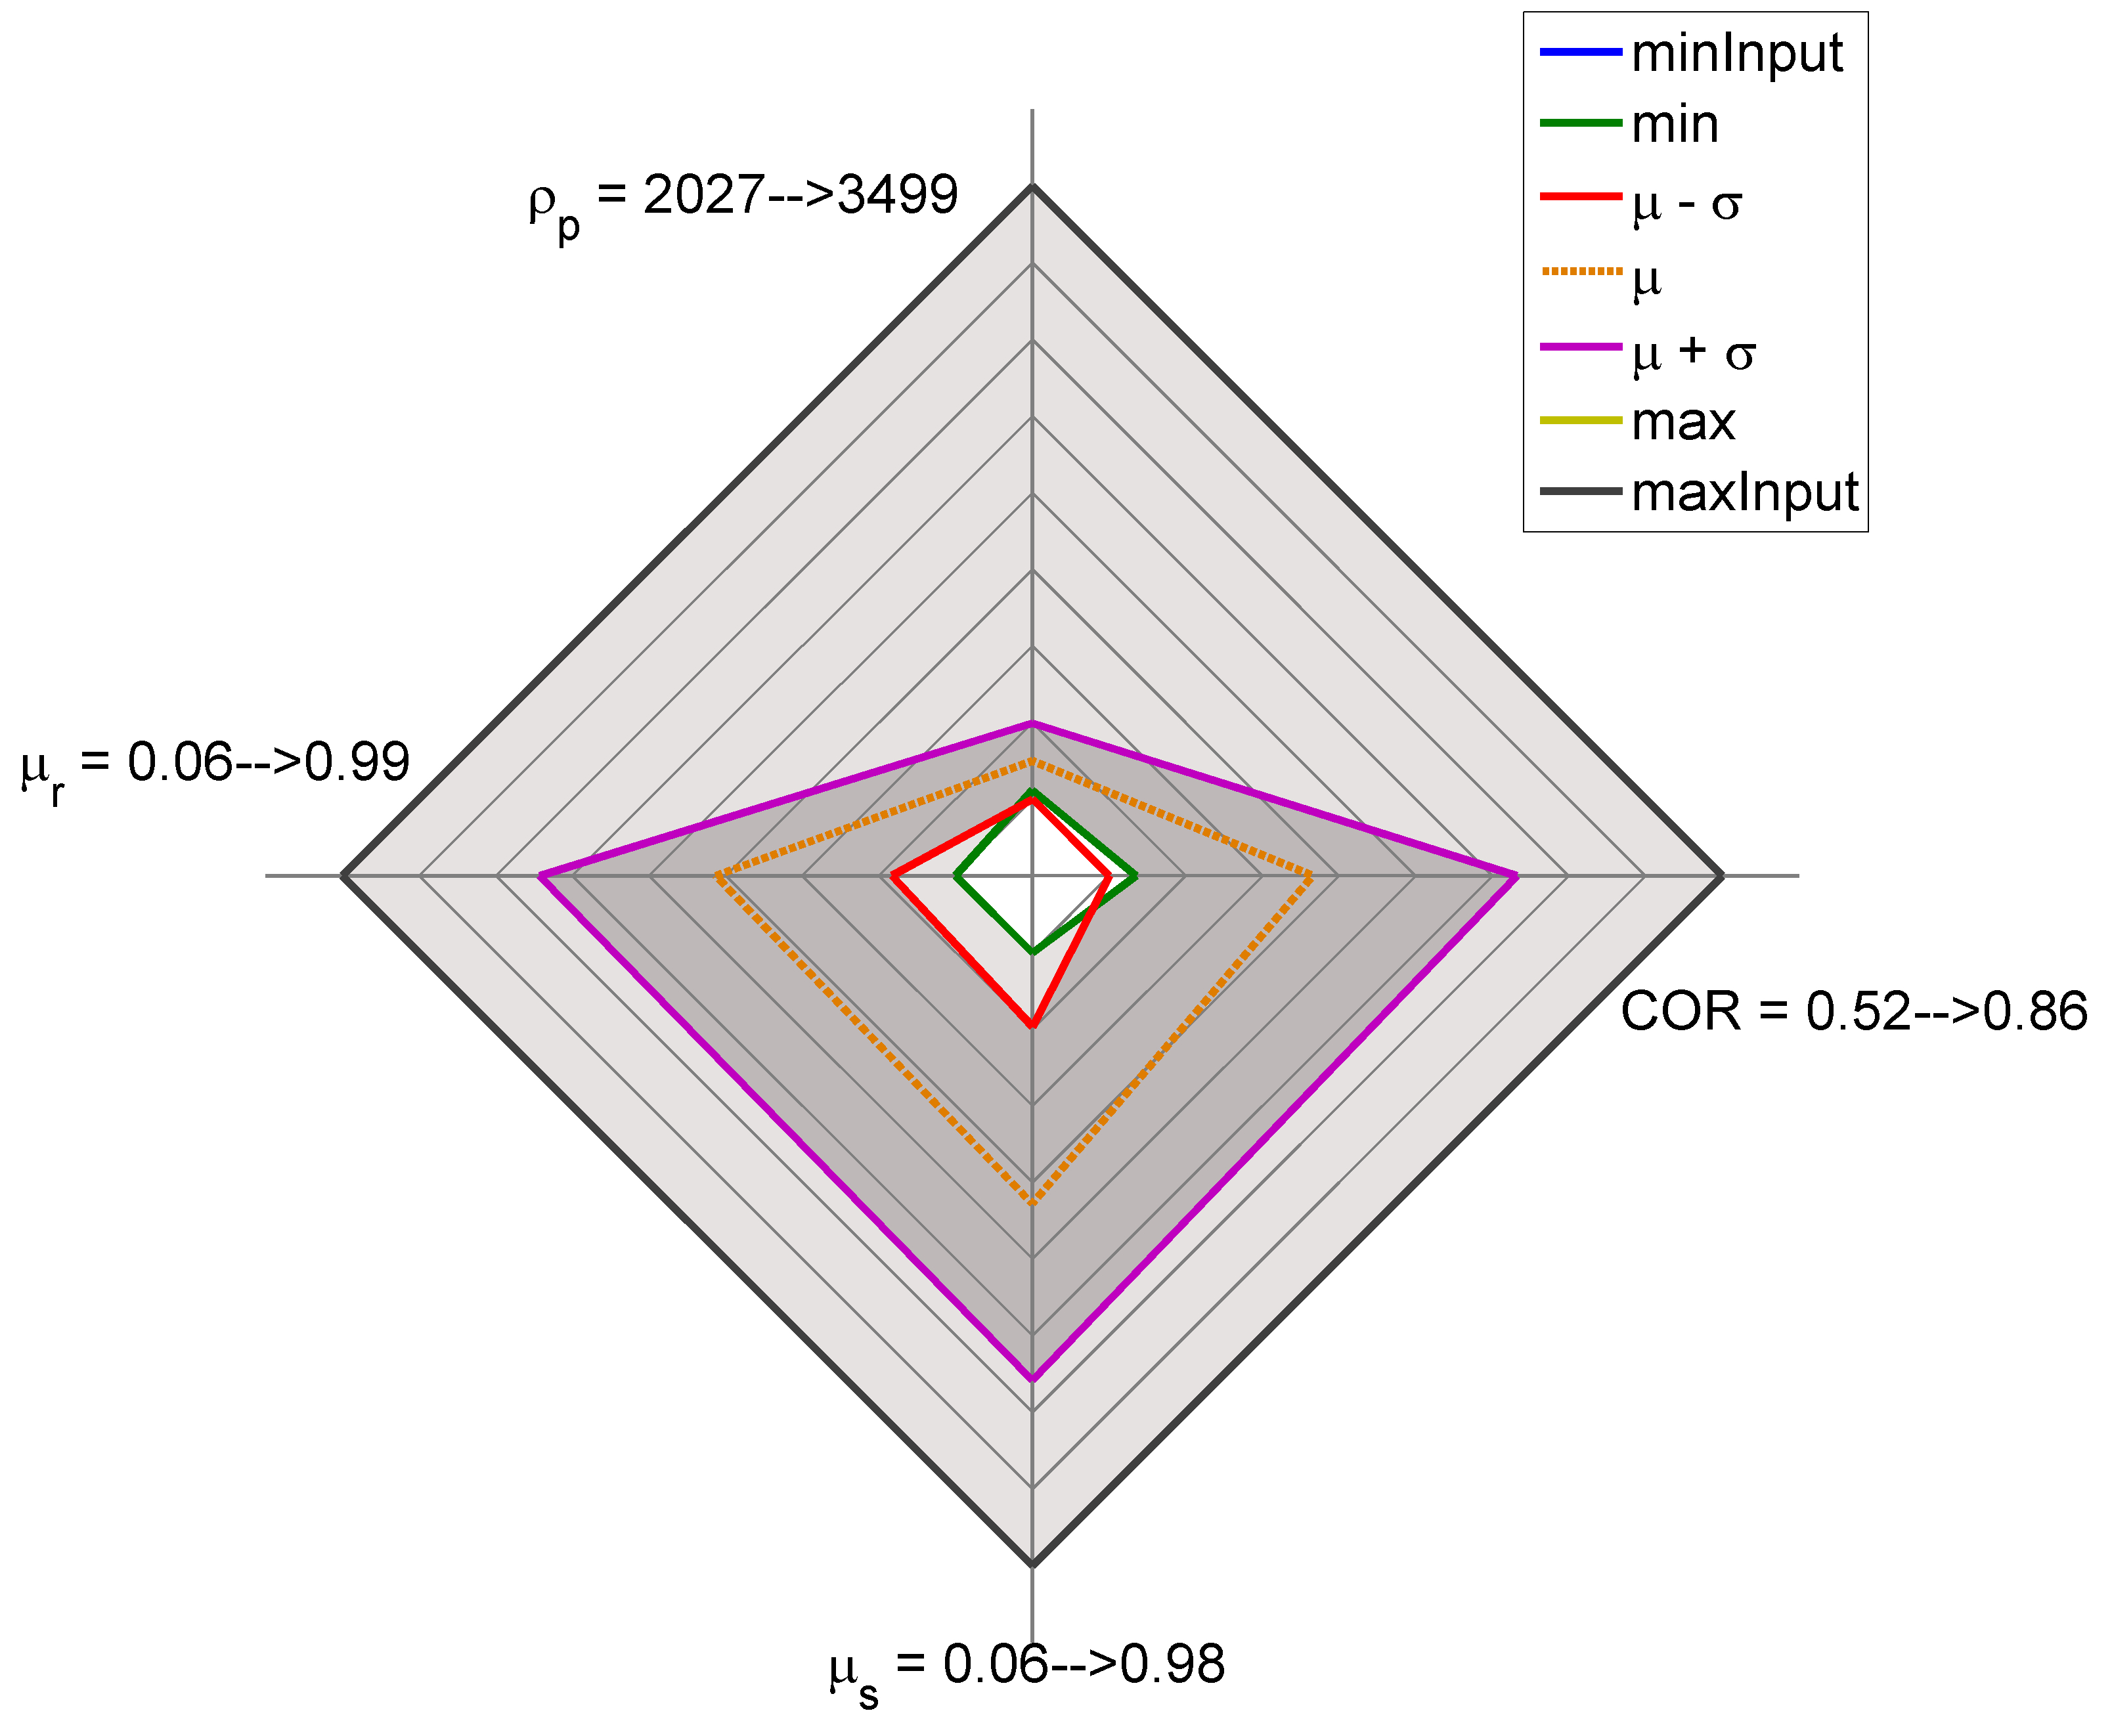
\includegraphics[width=.35\columnwidth]{images/041radarpirker1schulze1068}
	  \label{fig:041radarpirker1schulze1068}
  }
  \\
    \subfloat[Parameter space plot, \acs{SCT}, $\sigma_n=10070$ Pa, P=0.8.]{
	  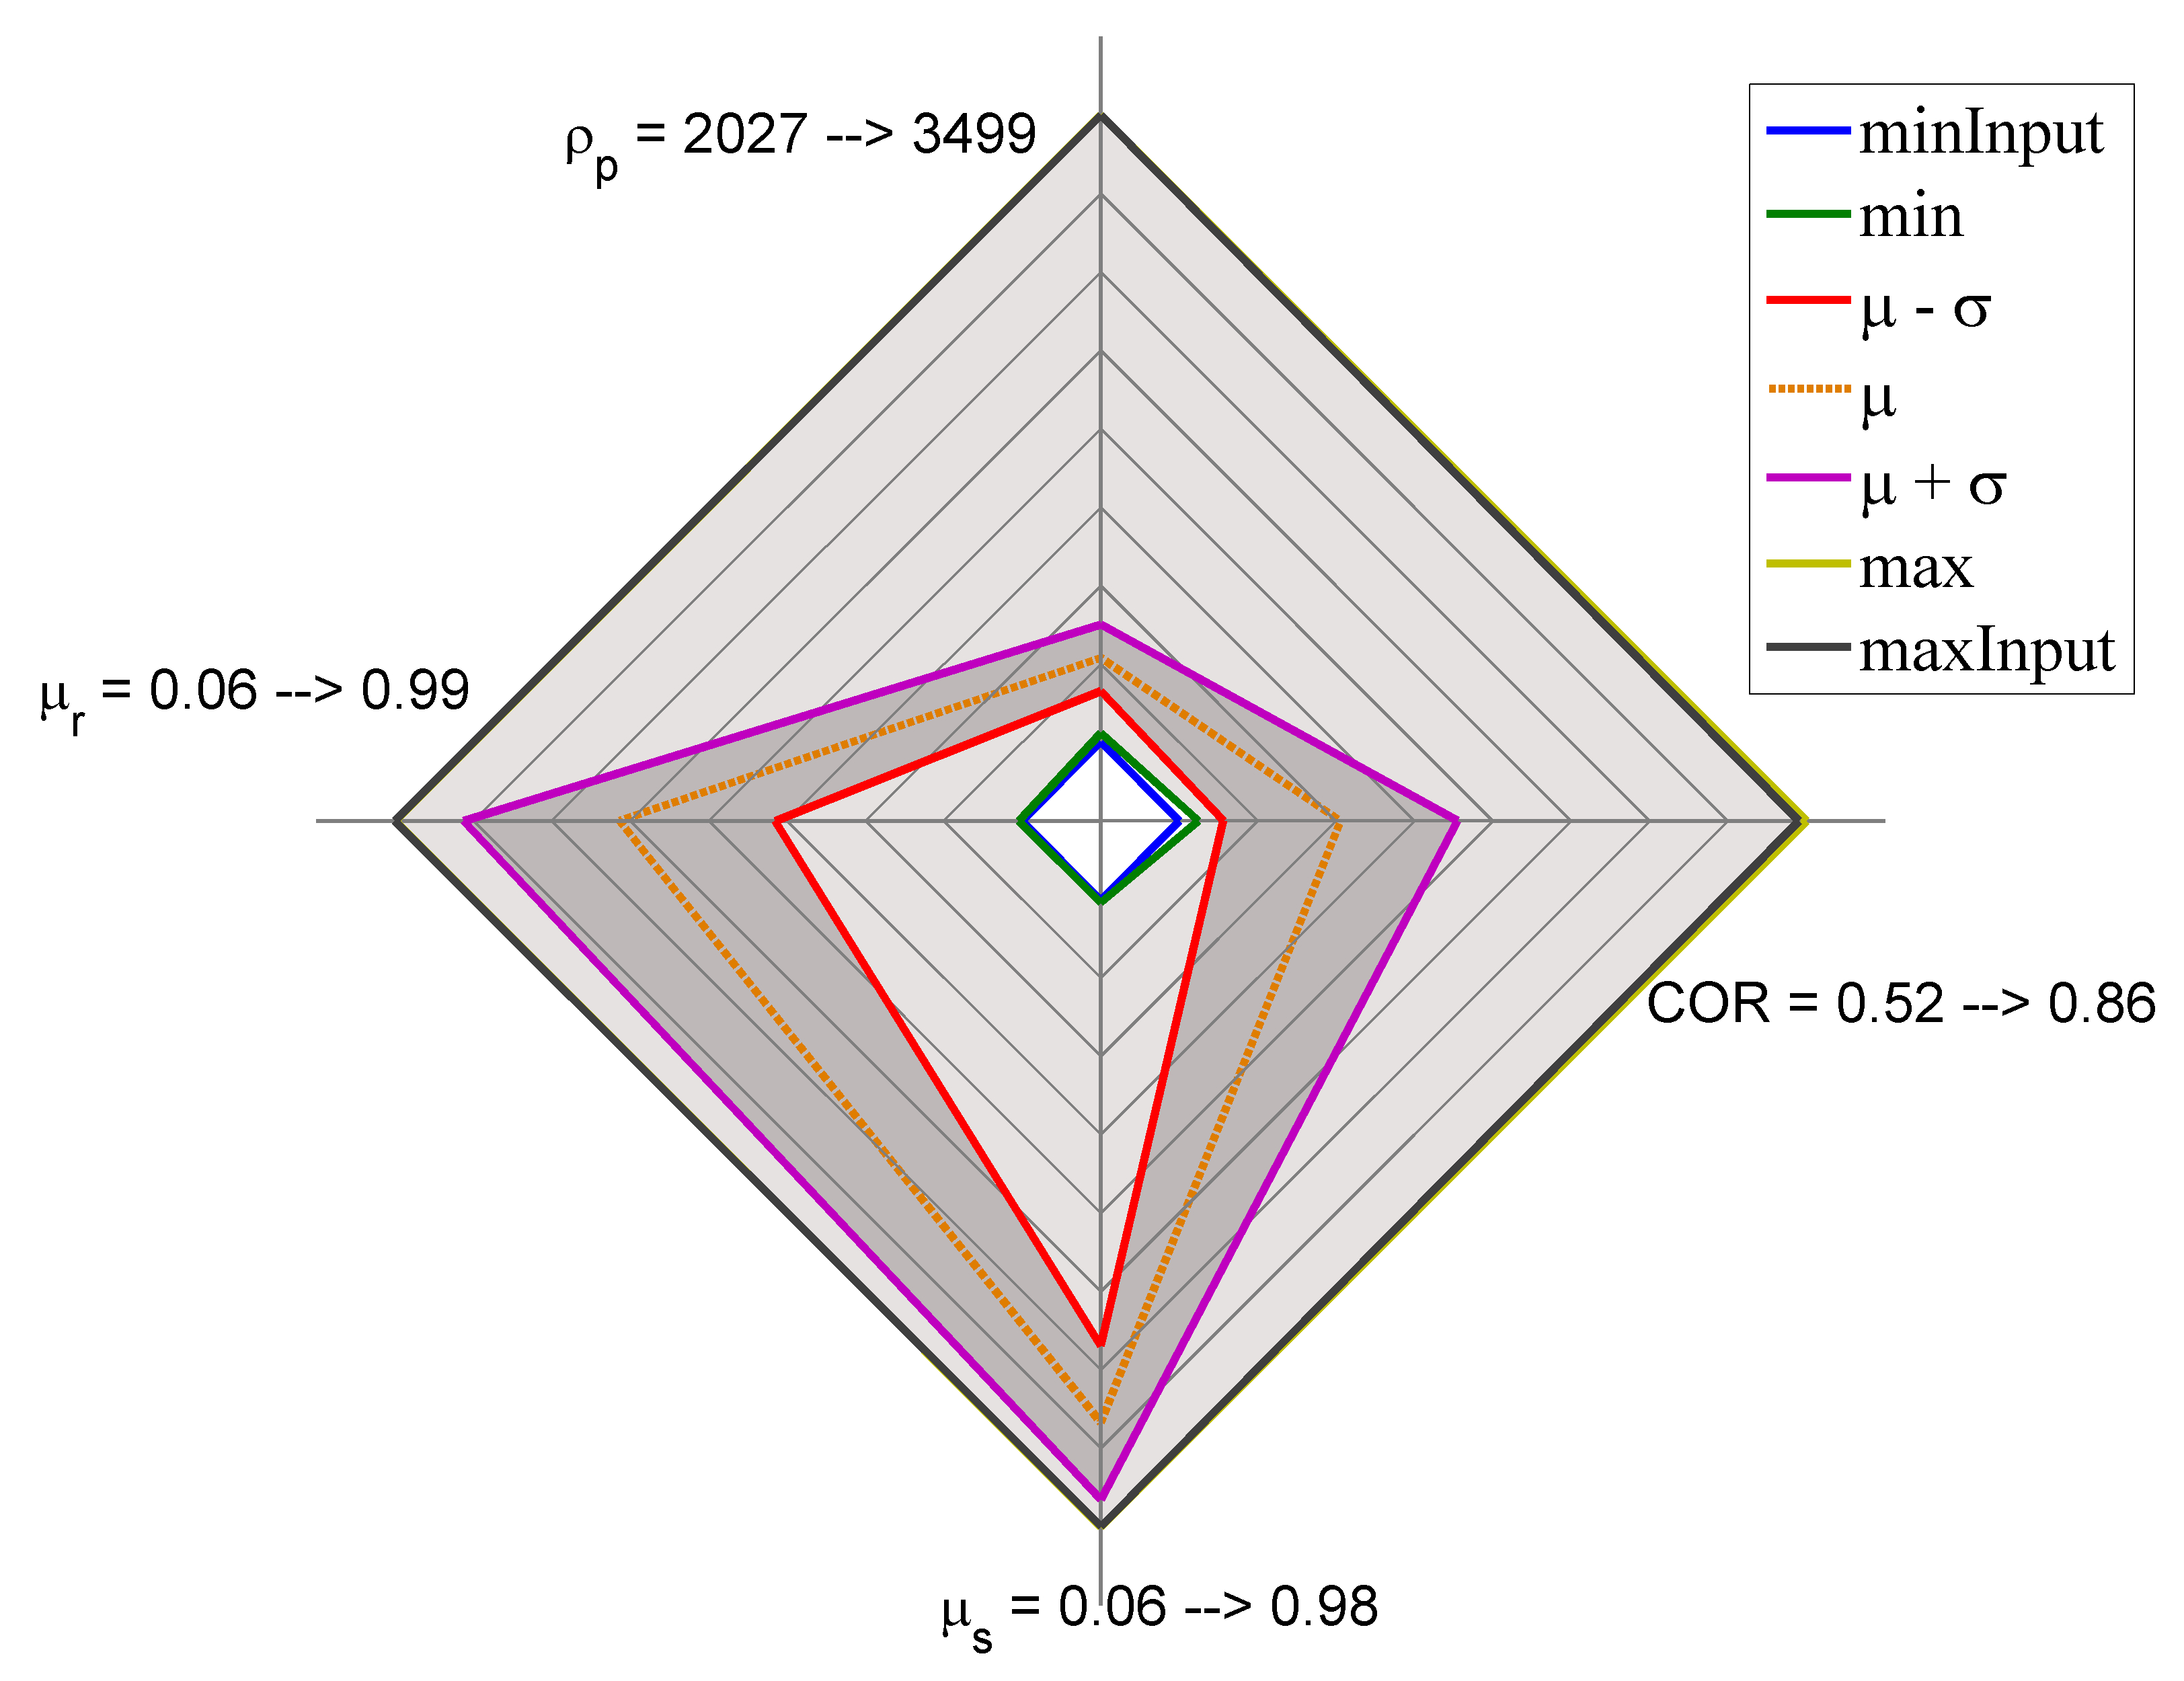
\includegraphics[width=.35\columnwidth]{images/026radarpirker08schulze10070}
	  \label{fig:026radarpirker08schulze10070}
  }
  \\
  \subfloat[Parameter space plot, \acs{SCT}, $\sigma_n=10070$ Pa, P=1.0.]{
	  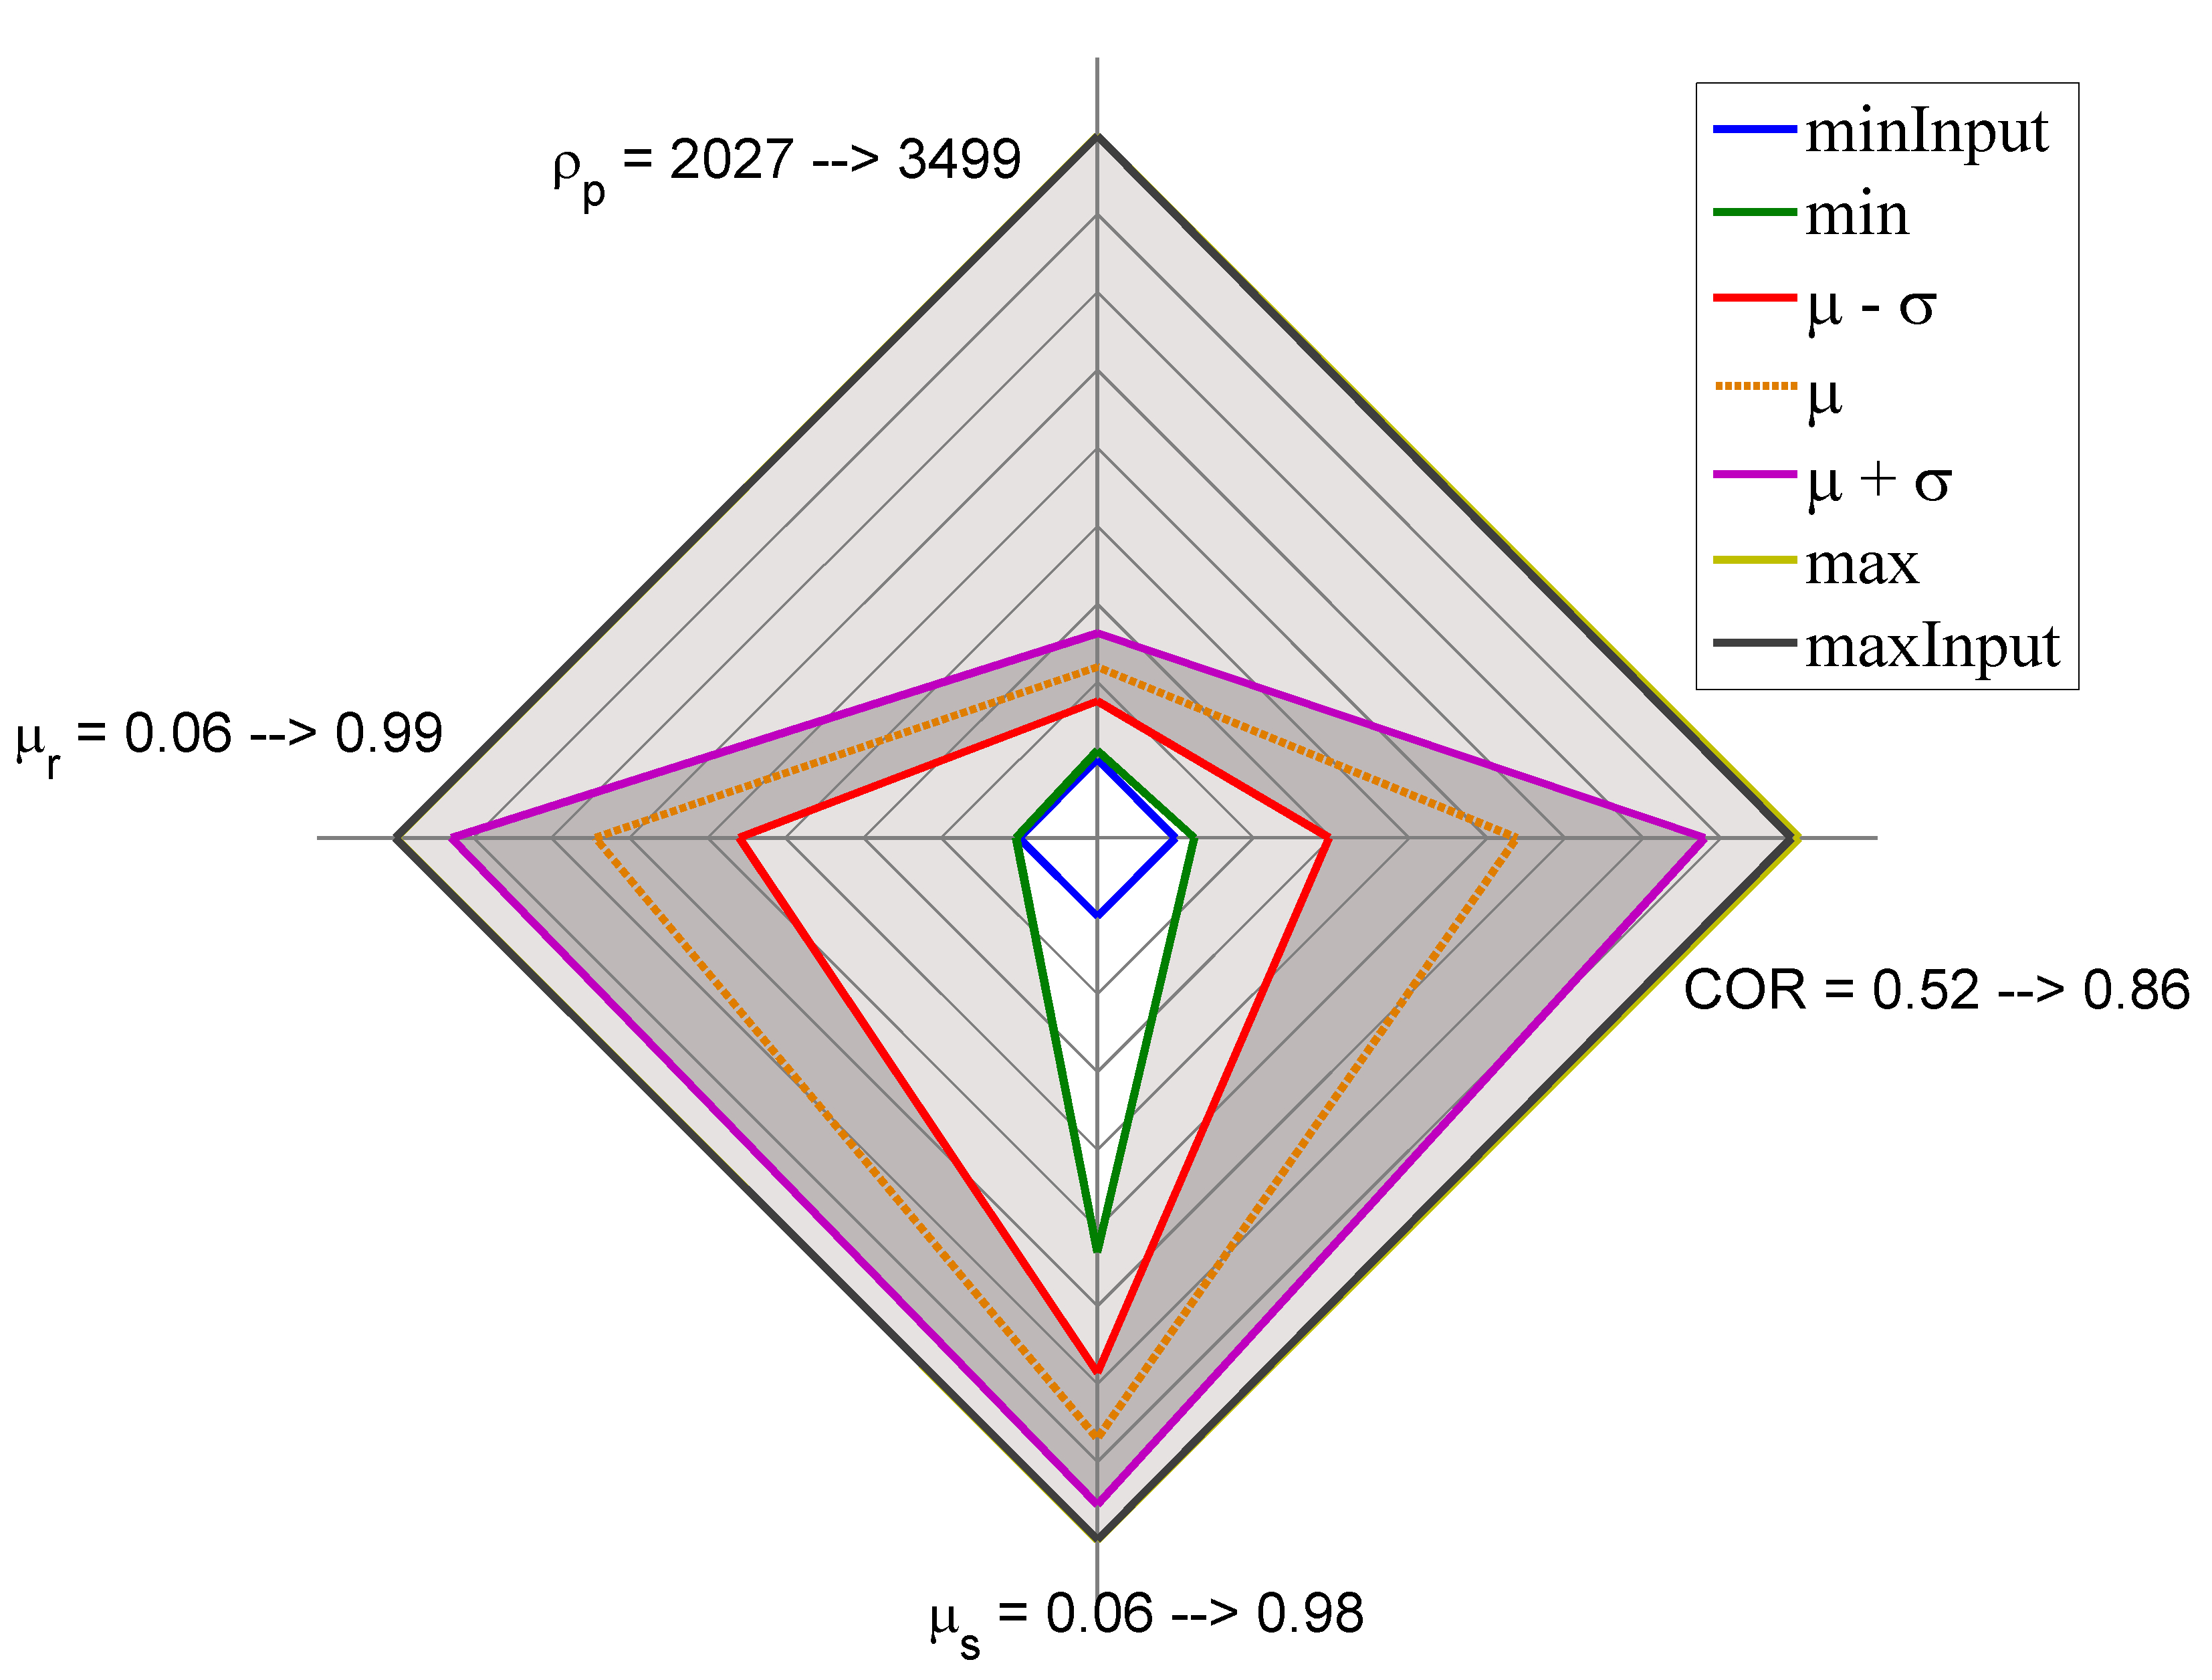
\includegraphics[width=.35\columnwidth]{images/024radarpirker1schulze10070}
	  \label{fig:024radarpirker1schulze10070}
  }
  \quad
    \subfloat[Box plot, \acs{SCT}, $\sigma_n=10070$ Pa, P=1.0.]{
	  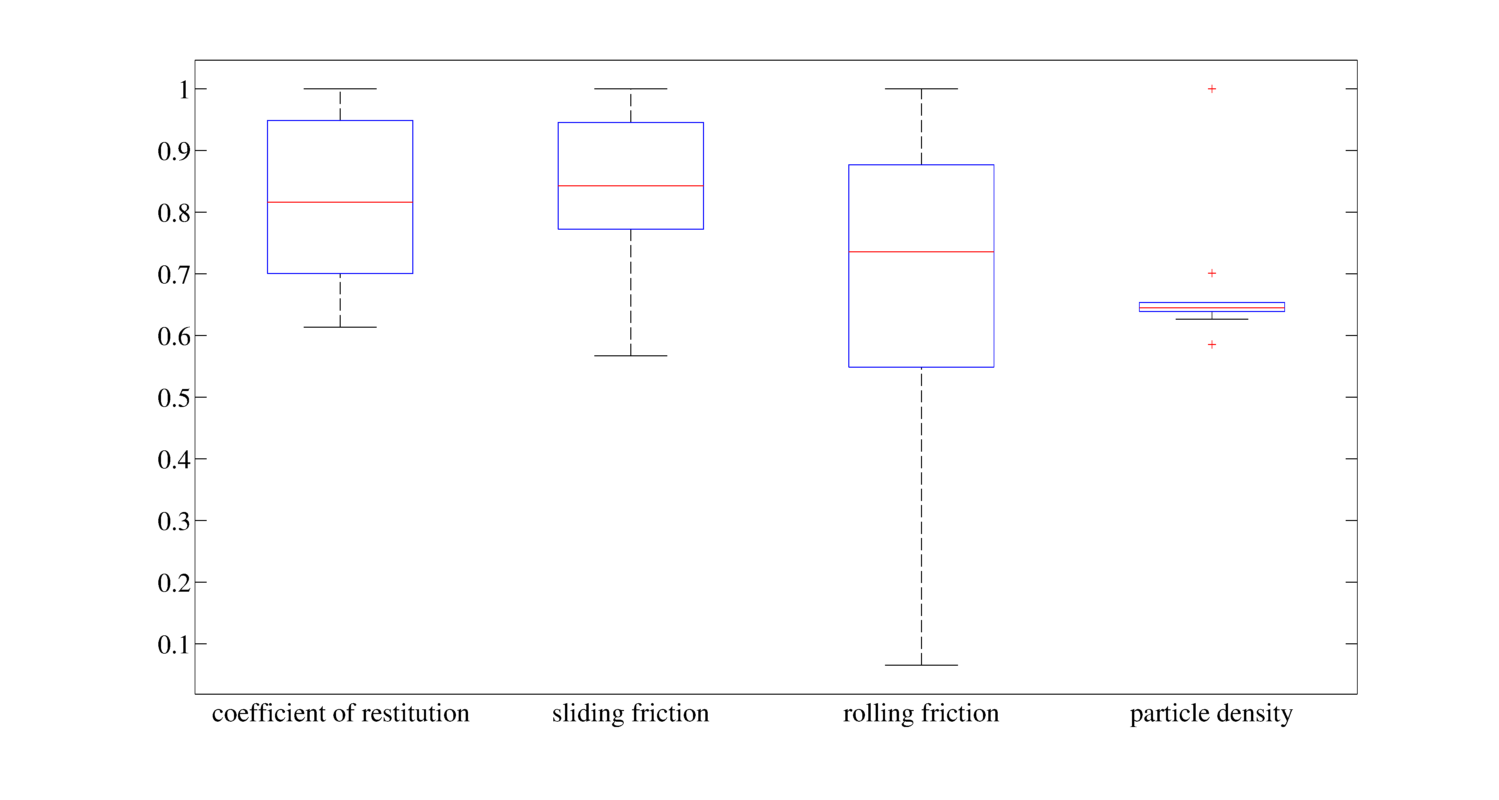
\includegraphics[width=.35\columnwidth]{images/075sctboxplot}
	  \label{fig:075sctboxplot}  }
  \\
    \subfloat[Parameter space plot, \acs{SCT}, $\sigma_n=10070$ Pa, P=1.2.]{
	  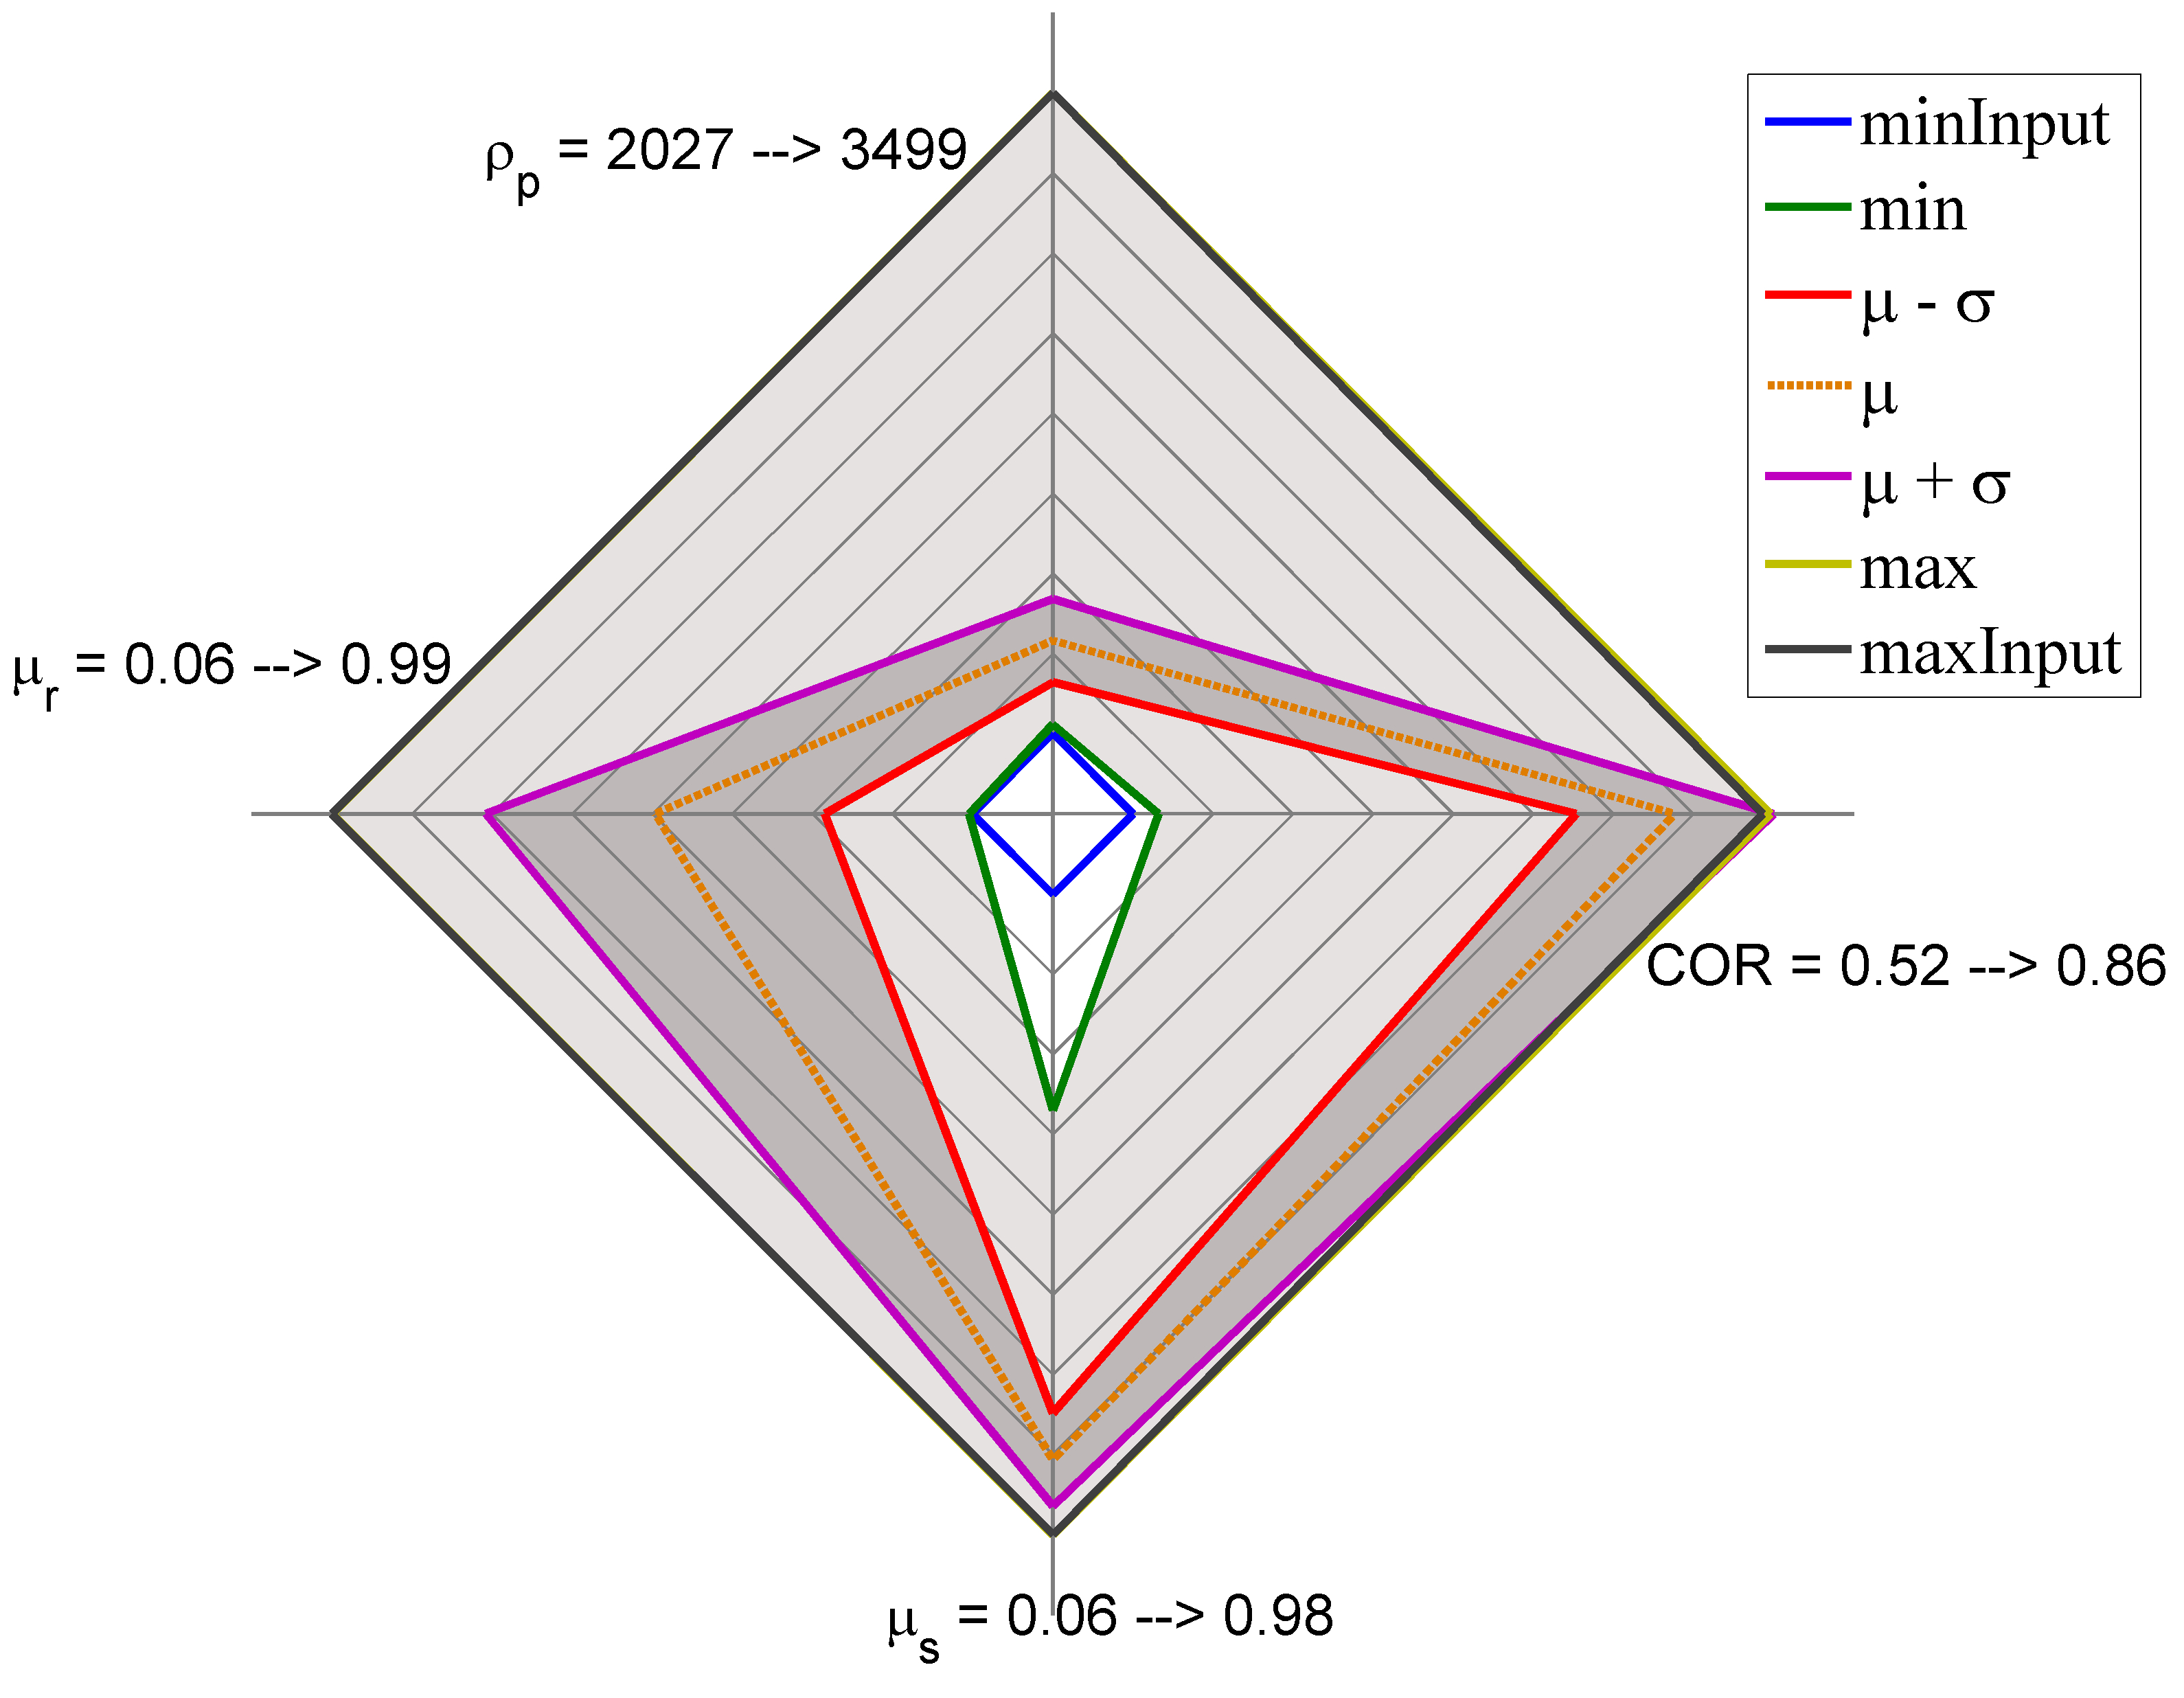
\includegraphics[width=.35\columnwidth]{images/028radarpirker12schulze10070}
	  \label{fig:028radarpirker12schulze10070}
  }
  \caption{SCT parameter space plots.}
  \label{fig:079sctparameterspaceplots}
\end{figure}

\subsection{Box plot}
\label{subsec:boxplot}
  
An example of a box plot can be seen
in Fig. \ref{fig:145BoxSCT1068p08sinterfine}.
\citet{RefWorks:207} defines a box plot a graphical representation of
collections of numerical data by means of their quartiles.
These are three points, which divide the data in four groups that are equals and
contain a quarter of the data each.\\
In a box plot the values between the first quartile (25\%) and the third
quartile (75\%) are included in a blue box.
Further, so called \textit{baffles} or \textit{whishers} are lines, which are
extended as far as the minimum and maximum values not considered outliers.
The data which exceed the whishers are represented with red crosses.
Finally, the median is represented as a red straight line.
Values are normalized, meaning that for each input value the maximum extracted
is one.\\
The representation through box plots in Fig.
\ref{fig:075sctboxplot} is consistent for the the \acs{rhop} and the
\acs{mus} with those shown in the parameter space plot in Fig.
\ref{fig:024radarpirker1schulze10070}.
However, the box plot representation helps to underline the much higher level of
variability for the \acs{mur} compared to the \acs{CoR}.
This can be explained if we consider again the non-unicity of the solution and
how the \acs{mur} has a reduced influence on the shear cell results compared to
the \acs{mus}.
This aspect is even clear in a density plot.

\begin{figure}[htbp]
\centering 
%   \subfloat[Parameter space plot, \acs{SCT}, $\sigma_n=1068$ Pa, P=1.0.]{
% 	  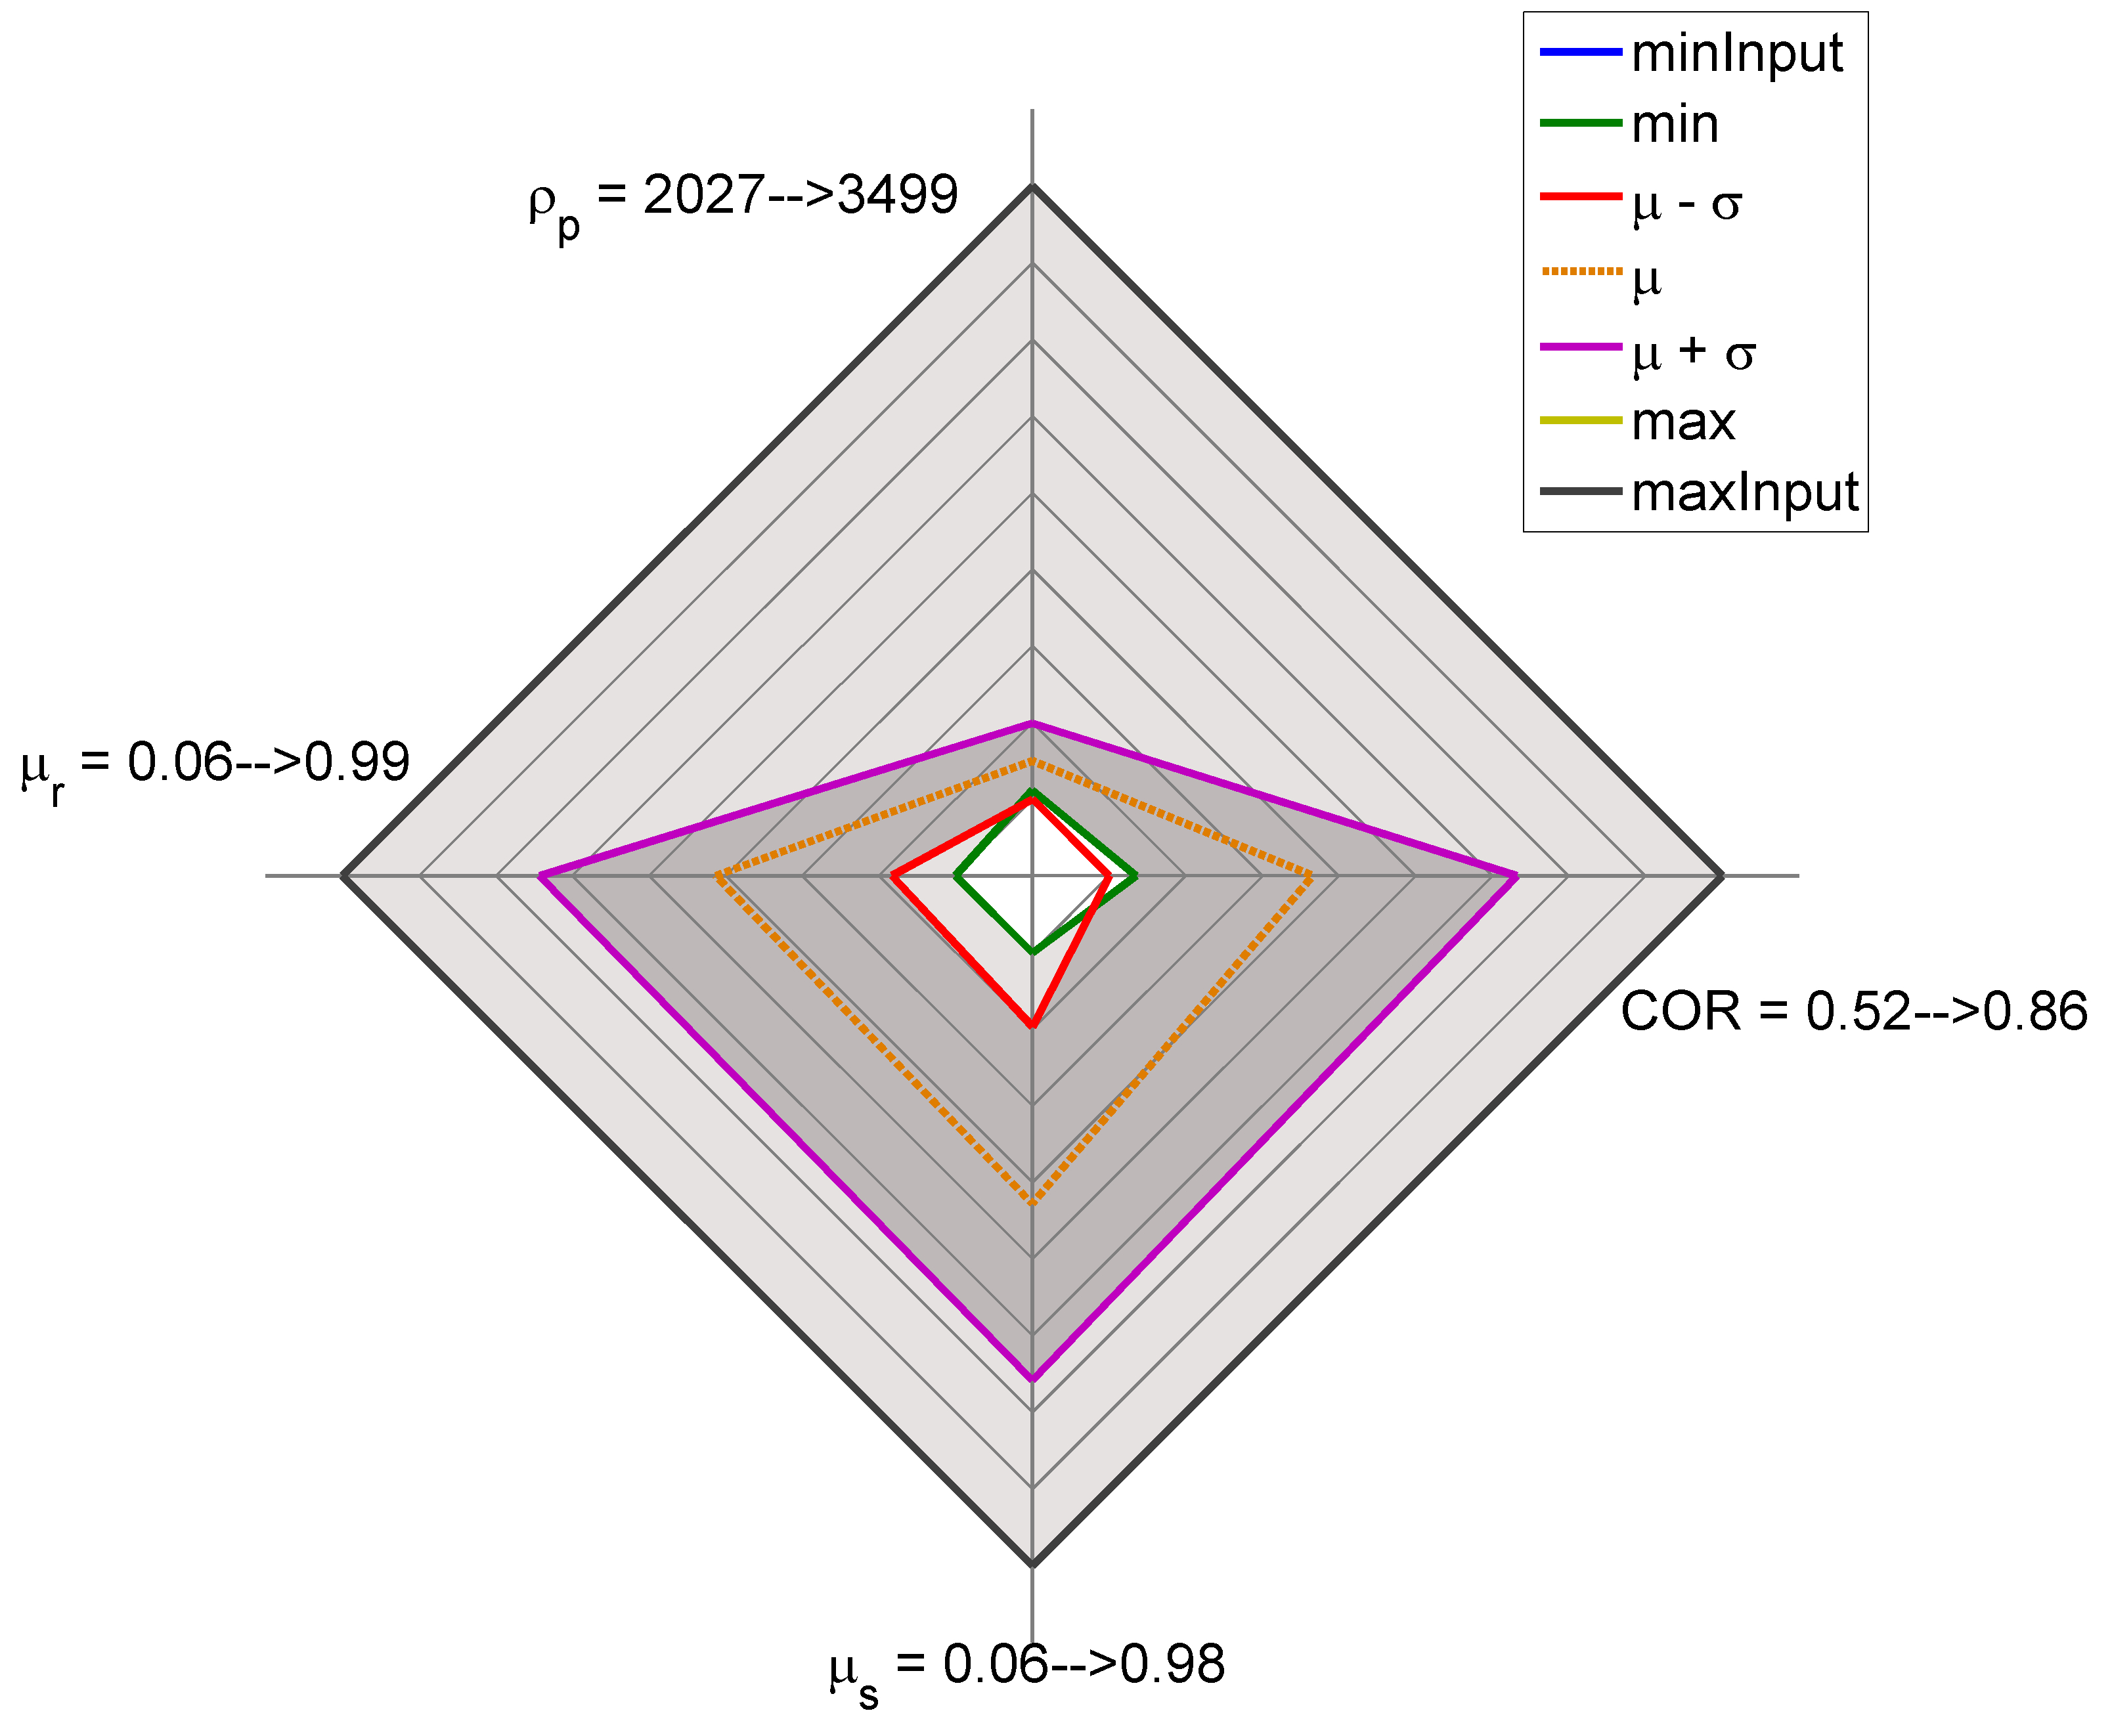
\includegraphics[width=.35\columnwidth]{images/041radarpirker1schulze1068}
% 	  \label{fig:041radarpirker1schulze1068}
%   }
%   \\157BoxSCT10070p08sinterfine.png
%158BoxSCT10070p12sinterfine.png
    \subfloat[Box plot, \acs{SCT}, $\sigma_n=10070$ Pa, P=0.8.]{
	  \includegraphics[width=.70\columnwidth]{images/157BoxSCT10070p08sinterfine}
	  \label{fig:157BoxSCT10070p08sinterfine}  }
  \\
    \subfloat[Box plot, \acs{SCT}, $\sigma_n=10070$ Pa, P=1.0.]{
	  \includegraphics[width=.70\columnwidth]{images/075sctboxplot}
	  \label{fig:075sctboxplot}  }
  \\
    \subfloat[Box plot, \acs{SCT}, $\sigma_n=10070$ Pa, P=1.2.]{
	  \includegraphics[width=.70\columnwidth]{images/158BoxSCT10070p12sinterfine}
	  \label{fig:158BoxSCT10070p12sinterfine}  }
  \\
  \caption[SCT box plots for sinter fine]{SCT box
  plots for sinter fine, $\sigma_n=10070$ Pa. The range of valid parameters is
  shown, together with the average and the 25 and 75 percentile.}
  \label{fig:156boxplotsct10070sinterfine}
\end{figure}

\subsection{Density plot}
\label{subsec:densityplot}

Further, we observed that various \acs{DEM} parameter
combinations could reproduce the experimental behaviour, and thus evaluated
their mutual dependencies.
This is shown more clearly in a density plot (e.g., Fig. 
\ref{fig:159TileSCT10070p08sinterfine}) 
of the particles' coefficient of restitution (\acs{CoR}) in relation to
the coefficients of sliding friction (\acs{mus}) and rolling friction (\acs{mur}).
The \acs{rhop} was not considered, since every valid combination has the same
value for it (or a close number).\\
In the white area, no valid sets of simulation parameters could be found.
In each cell the valid sets are grouped according to the 4 different COR
ranges.
Each cell is coloured according to the group with the most members.\\
It is clear their correlation, as already stated by Wensrich and 
Katterfeld \cite{RefWorks:87}.
For high values of the \acs{CoR} small values for \acs{mus} and \acs{mur} are
sufficient to reach the desired frictional bulk values.
On the other hand, with low \acs{CoR} values, high numbers for the friction
micro coefficients are necessary to achieve the same results.
This effect agrees with the contact law used, described in Chapter
\ref{cap:dem}.\\
For the $\acs{sigman} = 10,070$ Pa, P=1.0 case, Fig.
\ref{fig:160TileSCT10070p10sinterfine}, multiple
combinations (250,407 or 4\% of the total) of \acs{mus} and \acs{mur} reproduced
the experimental behaviour with varying \acs{CoR}.

\begin{figure}[htbp]
\centering 
  \subfloat[Density plot, $SSC$, $\sigma_n=10070$ Pa, P=0.8.]{
	  \includegraphics[width=.48\columnwidth]{images/027cloudpirker08schulze10070}
	  \label{fig:027cloudpirker08schulze10070}
  }
  \\
    \subfloat[Density plot, $SSC$, $\sigma_n=10070$ Pa, P=1.0.]{
	  \includegraphics[width=.48\columnwidth]{images/025cloudpirker1schulze10070}
	  \label{fig:025cloudpirker1schulze10070}
  }
  \\
  \subfloat[Density plot, $SSC$, $\sigma_n=10070$ Pa, P=1.2.]{
	  \includegraphics[width=.48\columnwidth]{images/030cloudpirker12schulze10070}
	  \label{fig:030cloudpirker12schulze10070}
  }
  \\
  \caption{Density plot comparison of SCT results.}
  \label{fig:080sctdensityplots}
\end{figure}

\subsection{Reliability Considerations}
\label{subsec:reliabilityconsiderations}

We tested the marked combinations
by modifying the experimental bulk values of the shear cell to further prove
the validity of the system.
We artificially decreased or increased the shear force, and thus \acs{mupsh} and
\acs{mush}, by a product coefficient ($P$), e.g. Eq. \ref{eq:pcoeff}:
\begin{equation}
\label{eq:pcoeff}
\mu_{psh, new} = \mu_{psh, old} \cdot P .
\end{equation}

First, we set it to $P=0.8$, and we obtained another
series of marked combinations ($MC2$).
It could be seen in the parameter space plot in Fig.
\ref{fig:026radarpirker08schulze10070} that the confidence range is narrower
than for $P=1.0$, while in the density plot in Fig. 
\ref{fig:159TileSCT10070p08sinterfine} the area
appears larger, although slightly less densely populated. Finally, for $P=1.2$
and its marked combinations ($MC3$) the parameter space plot in Fig.
\ref{fig:028radarpirker12schulze10070} shows a largely different confidence
range, while the density plot in Fig. \ref{fig:161TileSCT10070p12sinterfine} 
shows a smaller area. As expected, the procedure was highly sensitive to
variations in the experimental data.
Our approach could therefore be used
for a wide range of bulk materials.\\

%************************************************
%************************************************

\subsection{Sinter fine 1068}
\label{subsec:sinterfine1068}

\begin{figure}[htbp]
	\centering

    \subfloat[Parameter space plot, \acs{SCT}, $\sigma_n=1068$ Pa, P=0.8.]{
	  \includegraphics[width=.5\columnwidth]{images/150ParamSpaceSCT1068p08sinterfine}
	  \label{fig:150ParamSpaceSCT1068p08sinterfine}  }
	 
    \subfloat[Parameter space plot, \acs{SCT}, $\sigma_n=1068$ Pa, P=1.0.]{
	  \includegraphics[width=.5\columnwidth]{images/041radarpirker1schulze1068}
	  \label{fig:041radarpirker1schulze1068}  } 
	  
    \subfloat[Parameter space plot, \acs{SCT}, $\sigma_n=1068$ Pa, P=1.2.]{
	  \includegraphics[width=.5\columnwidth]{images/151ParamSpaceSCT1068p12sinterfine}
	  \label{fig:151ParamSpaceSCT1068p12sinterfine}  } 	  
	  

 % \hfill\null
  \caption[SCT parameter space plots 1]{SCT parameter space
  plots for sinter fine, $\sigma_n=1068$ Pa.}
  \label{fig:149paramspaceplotsct1068}
\end{figure}

% \begin{figure}%[!h] 
% \centering 
% \includegraphics[width=.80\columnwidth]{images/022regression.eps}
% %[width=.48\textwidth]
% \caption[Comparison between prediction of the trained ANN and full DEM
% simulation]{Comparison between prediction of the trained Artificial Neural
% Network (\acs{ANN}) and 546 
% \wrong{write down all the simulations performed at the end.}
% full DEM simulations of the coefficient of pre-shear
% (\acs{mupsh}).}
% \label{fig:022regression} 
% \end{figure}
\begin{figure}[htbp]
	\centering

    \subfloat[Box plot, \acs{SCT}, $\sigma_n=1068$ Pa, P=0.8.]{
	  \includegraphics[width=.75\columnwidth]{images/145BoxSCT1068p08sinterfine}
	  \label{fig:145BoxSCT1068p08sinterfine}  }
	 
    \subfloat[Box plot, \acs{SCT}, $\sigma_n=1068$ Pa, P=1.0.]{
	  \includegraphics[width=.75\columnwidth]{images/148BoxSCT1068p10sinterfine}
	  \label{fig:147BoxSCT1068p10sinterfine}  } 
	  
    \subfloat[Box plot, \acs{SCT}, $\sigma_n=1068$ Pa, P=1.2.]{
	  \includegraphics[width=.75\columnwidth]{images/147BoxSCT1068p12sinterfine}
	  \label{fig:148BoxSCT1068p12sinterfine}  } 	  
	  

 % \hfill\null
  \caption[SCT box plots 1]{SCT box
  plots for sinter fine, $\sigma_n=1068$ Pa.}
  \label{fig:146boxplotsct1068}
\end{figure}

% \begin{figure}%[!h] 
% \centering 
% \includegraphics[width=.80\columnwidth]{images/022regression.eps}
% %[width=.48\textwidth]
% \caption[Comparison between prediction of the trained ANN and full DEM
% simulation]{Comparison between prediction of the trained Artificial Neural
% Network (\acs{ANN}) and 546 
% \wrong{write down all the simulations performed at the end.}
% full DEM simulations of the coefficient of pre-shear
% (\acs{mupsh}).}
% \label{fig:022regression} 
% \end{figure}
\begin{figure}[htbp]
	\centering

    \subfloat[Density plot, \acs{SCT}, $\sigma_n=1068$ Pa, P=0.8.]{
	  \includegraphics[width=.75\columnwidth]{images/152TileSCT1068p08sinterfine}
	  \label{fig:152TileSCT1068p08sinterfine}  }
	 
    \subfloat[Density plot, \acs{SCT}, $\sigma_n=1068$ Pa, P=1.0.]{
	  \includegraphics[width=.75\columnwidth]{images/153TileSCT1068p10sinterfine}
	  \label{fig:153TileSCT1068p10sinterfine}  } 
	  
    \subfloat[Density plot, \acs{SCT}, $\sigma_n=1068$ Pa, P=1.2.]{
	  \includegraphics[width=.75\columnwidth]{images/154TileSCT1068p12sinterfine}
	  \label{fig:154TileSCT1068p12sinterfine}  } 	  
	  

 % \hfill\null
  \caption[SCT Density plots 1]{SCT Density
  plots for sinter fine, $\sigma_n=1068$ Pa.}
  \label{fig:155tileplotsct1068sinterfine}
\end{figure}

% \begin{figure}%[!h] 
% \centering 
% \includegraphics[width=.80\columnwidth]{images/022regression.eps}
% %[width=.48\textwidth]
% \caption[Comparison between prediction of the trained ANN and full DEM
% simulation]{Comparison between prediction of the trained Artificial Neural
% Network (\acs{ANN}) and 546 
% \wrong{write down all the simulations performed at the end.}
% full DEM simulations of the coefficient of pre-shear
% (\acs{mupsh}).}
% \label{fig:022regression} 
% \end{figure}

\subsection{AoR results}
\label{subsec:aorresults}

We then processed the random combinations with the \acs{AoR} \acs{ANN}. In Fig.
\ref{fig:031radarpirker1aor} the parameter space plot for the same criteria as
before could be seen.
In accordance with theory (Wensrich and Katterfeld \cite{RefWorks:87}), in a simulation dominated
by rolling particles, the coefficient of rolling friction has the maximum
influence. \\
\begin{figure}[htbp]
\centering 
  \subfloat[Parameter space plot, $AoR_{exp} = 38.85 ^\circ$.]{
	  \includegraphics[width=.50\columnwidth]{images/031radarpirker1aor}
	  \label{fig:031radarpirker1aor}
  }
  \\
    \subfloat[Box plot, $AoR_{exp} = 38.85 ^\circ$.]{
	  \includegraphics[width=.60\columnwidth]{images/076aorboxplot}
	  \label{fig:076aorboxplot}
  }
  \\
    \subfloat[Density plot plot, $AoR_{exp} = 38.85
        ^\circ$.]{
	  \includegraphics[width=.60\columnwidth]{images/162TileAORsinterfine}
	  \label{fig:162TileAORsinterfine}  }
  \\
  \caption[AoR valid values plots]{\acs{AoR} valid values plots. The valid
  values for the \acs{AoR} sinter fine test are shown in three different plots.
  The results are clearly different from the \acs{SCT} test and the \acs{mur}
  is the most relevant parameter.}
  \label{fig:207aorparameterspaceplots}
\end{figure}
%************************************************
% \begin{table}[h]
\centering
\begin{tabular}{cccccc}
\hline
$\sigma_n$ (Pa) & $\tau$ (Pa) & $\mu_{psh}$ (-) & $\tau_{\%}$ (\%) &
$\mu_{sh}$ (-) & $\rho_b$ (kg/m3) \\
\hline
    1068  & 1059  & 0.9916 & 80 & 1.2333 & 1718 \\
    2069  & 1818  & 0.8787 & 80 & 0.9994 & 1759 \\
    10070 & 8232  & 0.8175 & 80 & 1.1712 & 1802 \\

\hline
\end{tabular}
\caption[Experimental results]{Experimental results. Values for three
load conditions}
\label{tab:05sinterTableExperimental}
\end{table}
% \info{one table for each material? here or in the polydispersity chapter?}

\subsection{Merge results}
\label{subsec:mergeresults}

Finally, we extracted from the $MC1$ values the \acs{AoR} \acs{ANN} behaviour
and compared it with the experimental one.
As could be seen in the parameter space plot in Fig.
\ref{fig:208mergeparameterspaceplots}, the confidence interval is very small,
indicating that all the parameters but the \acs{CoR} played an important role, 
and demonstrating the reliability of these parameter
combinations in representing the bulk behaviour.
From the initial 6,250,000 combinations, only 3,884 were valid (0.0621
\%), see Table \ref{tab:13DEMvalidvalues}.

\begin{table}[h]
\centering
\begin{tabular}{llccc}
\hline

          & type  & SSC & AoR   & SSC \& AoR \\
          \hline

    $\mu_s$ & mean  & 0.831 & 0.177 & 0.664 \\
    $[-]$   & std. dev. (SD) & 0.097 & 0.095 & 0.029 \\
          & range ($R$) & 0.9   & 0.9   & 0.9 \\
          & SD / R & 0.108 & 0.106 & 0.032 \\
          \hline
    $\mu_r$ & mean  & 0.692 & 0.830 & 0.916 \\
    $[-]$   & std. dev. (SD) & 0.215 & 0.193 & 0.042 \\
          & range ($R$) & 0.9   & 0.9   & 0.9 \\
          & SD / R & 0.239 & 0.214 & 0.046 \\
          \hline
              COR   & mean  & 0.708 & 0.590 & 0.590 \\
   $ [-]$   & std. dev. (SD) & 0.104 & 0.073 & 0.065 \\
          & range ($R$) & 0.4   & 0.4   & 0.4 \\
          & SD / R & 0.259 & 0.183 & 0.161 \\
          \hline
    $\rho_p$ & mean  & 2245.7 & 3192.8 & 2283.9 \\
    $[kg/m3]$ & std. dev. (SD) & 80.5  & 277.4 & 67.1 \\
          & range ($R$) & 1500  & 1500  & 1500 \\
          & SD / R & 0.054 & 0.185 & 0.045 \\
          \hline
    valid & number & 290203 & 816552 & 3884 \\
    combinations & [$\%$] & 4.64  & 13.06 & 0.06 \\  

\hline
\end{tabular}
\caption[DEM valid values]{DEM valid values. For each parameter we show the
valid parameters statistics in the two tests and in their intersection.
Finally, we show the number of valid parameters combinations over the total
(6250000).}
\label{tab:13DEMvalidvalues}
\end{table}
\begin{figure}[htbp]
\centering 
  \subfloat[Parameter space plot, $AoR_{exp} = 38.85 
        ^\circ$ \& \acs{SCT}: $\sigma_n=10070$ Pa.]{
	  \includegraphics[width=.50\columnwidth]{images/033radarpirker1schulze10070aor}
	  \label{fig:033radarpirker1schulze10070aor}
  }
  \\
    \subfloat[Box plot, $AoR_{exp} = 38.85
        ^\circ$ \& \acs{SCT}: $\sigma_n=10070$ Pa.]{
	  \includegraphics[width=.60\columnwidth]{images/078mergeboxplot}
	  \label{fig:078mergeboxplot}  }
  \\
  \subfloat[TIle plot, $AoR_{exp} = 38.85 
        ^\circ$ \& \acs{SCT}: $\sigma_n=10070$ Pa.]{
	  \includegraphics[width=.60\columnwidth]{images/206TileMixsinterfine_33}
	  \label{fig:206TileMixsinterfine_33}
  }
  \\  
  \caption{Merge parameter space plots.}
  \label{fig:208mergeparameterspaceplots}
\end{figure}


%************************************************
%************************************************

\section{Remaining Materials Characterization}
\label{sec:remainingmaterialscharacterization}

We later proceeded in further expanding the characterization by investigating
the values for the remaining materials.
Thus, we realized a limited number of simulations (620 \acs{SCT} simulations
and 180 \acs{AoR} simulations) with the particles distributions in Table
\ref{tab:19particlesizedistributions} and the stress conditions in Table
\ref{tab:21shearcell2}.\\
Together with the simulations already performed for sinter fine, we trained
additional \acs{ANNs} for the four bulk values involved.
Again, we extracted those with the maximum \acs{r2}.
The weights and biases for the \acs{muie} can be found in Table
\ref{tab:33weightsbiasesmuie}.
Similarly, weights and biases for the \acs{AoR} are in Table
\ref{tab:32weightsbiasesAOR}.

\begin{sidewaystable}[htbp] 
 \centering 
\begin{tabular}{l|ccccccccccccccc} 
 \hline 
   &    \multicolumn{15}{l}{Weights of connection between input and hidden layer}  \\ 
 Neurons & 1 &  2 &  3 &  4 &  5 &  6 &  7 &  8 & 9 & 10 & 11 & 12 & 13 & 14 & 15  \\ 
 \hline 
  & 0.407 &  -0.055 &  -1.384 &  0.616 &  -0.436 &  -1.082 &  -0.155 &  0.667 &  -0.071  &  -0.567 &  1.388 &  -0.367 &  0.796 &  -0.815 &  1.607 \\ 
  & 0.242 &  -1.367 &  -1.057 &  -1.475 &  1.112 &  0.049 &  -0.002 &  0.688 &  0.517  &  1.395 &  0.009 &  -1.091 &  0.845 &  0.163 &  -0.122 \\ 
  & -0.045 &  0.866 &  0.026 &  0.012 &  0.277 &  0.221 &  -0.008 &  0.358 &  0.473  &  0.037 &  -0.004 &  -0.405 &  -0.507 &  -0.154 &  -0.170 \\ 
  & 0.803 &  0.001 &  -0.158 &  -0.039 &  0.491 &  -0.255 &  0.779 &  -0.004 &  -0.734  &  -0.339 &  -0.257 &  -0.862 &  -0.014 &  -1.375 &  0.403 \\ 
  & -1.984 &  -0.734 &  0.533 &  0.182 &  0.754 &  0.861 &  -0.627 &  0.790 &  -0.505  &  0.048 &  -0.262 &  0.093 &  0.160 &  0.810 &  -0.038 \\ 
  & 0.092 &  -0.320 &  -0.327 &  -0.046 &  -0.596 &  0.175 &  0.805 &  -1.232 &  1.130  &  0.601 &  0.303 &  0.505 &  -1.295 &  0.245 &  -0.347 \\ 
  & -0.285 &  -0.094 &  1.291 &  -0.007 &  -0.352 &  -0.947 &  0.077 &  0.452 &  0.557  &  -0.245 &  -0.096 &  -1.089 &  0.297 &  -1.300 &  -0.340 \\ 
  & -0.058 &  0.250 &  -0.061 &  -0.147 &  -0.864 &  0.893 &  0.422 &  0.690 &  -0.246  &  -0.239 &  -0.036 &  0.569 &  0.448 &  -0.639 &  1.007 \\ 
\hline 
   &    \multicolumn{15}{l}{Weights of connection between hidden and output layer}  \\ 
  & 1.114 &  -0.026 &  -0.156 &  -0.348 &  -0.024 &  -0.024 &  -0.172 &  0.065 &  -0.085  &  -0.121 &  0.404 &  -0.057 &  -0.083 &  -0.117 &  0.009 \\ 
\hline 
   &    \multicolumn{15}{l}{Biases of hidden layer}  \\ 
  & -2.744 &  -1.815 &  1.032 &  -1.501 &  0.845 &  0.385 &  0.324 &  -0.113 &  -0.567  &  -0.573 &  1.114 &  -0.982 &  1.564 &  -1.068 &  1.630 \\ 
\hline 
   &    \multicolumn{15}{l}{Biases of output layer}  \\ 
 &    \multicolumn{15}{c}{0.151}  \\ 
\hline 
 \end{tabular} 
\caption[Weights and biases table for coefficient of internal friction]{Weights and biases table for coefficient of internal friction.} 
\label{tab:33weightsbiasesmuie} 
\end{sidewaystable}
\begin{table}[htbp] 
 \centering 
\begin{tabular}{l|ccccccccc} 
 \hline 
   &    \multicolumn{9}{l}{Weights of connection between input and hidden layer}  \\ 
 Neurons & 1 &  2 &  3 &  4 &  5 &  6 &  7 &  8 & 9 \\ 
 \hline 
  & 1.312 &  -1.389 &  -1.470 &  0.368 &  -0.259 &  -0.014 &  3.356 &  -0.692 &  0.446 \\ 
  & -1.729 &  0.699 &  -0.660 &  0.622 &  0.769 &  1.156 &  0.488 &  -0.656 &  0.601 \\ 
  & -0.539 &  -1.052 &  0.228 &  -0.535 &  -0.180 &  -0.870 &  -0.149 &  0.672 &  -0.721 \\ 
  & 0.029 &  -0.100 &  0.357 &  -1.181 &  1.490 &  -0.777 &  0.016 &  -0.824 &  -0.620 \\ 
  & -0.022 &  -0.173 &  0.597 &  1.444 &  0.736 &  1.141 &  -0.029 &  -1.045 &  -0.859 \\ 
  & 0.192 &  -0.239 &  0.320 &  -0.151 &  0.357 &  -0.464 &  -0.042 &  -0.759 &  0.735 \\ 
\hline 
   &    \multicolumn{9}{l}{Weights of connection between hidden and output layer}  \\ 
  & -0.512 &  0.242 &  -0.098 &  0.030 &  -0.068 &  -0.003 &  0.750 &  -0.013 &  -0.010 \\ 
\hline 
   &    \multicolumn{9}{l}{Biases of hidden layer}  \\ 
  & -2.204 &  1.678 &  0.999 &  -0.526 &  -0.294 &  -0.298 &  0.683 &  -1.631 &  2.343 \\ 
\hline 
   &    \multicolumn{9}{l}{Biases of output layer}  \\ 
 &    \multicolumn{9}{c}{-0.739}  \\ 
\hline 
 \end{tabular} 
\caption[Weights and biases table for AOR]{Weights and biases table for AOR.} 
\label{tab:32weightsbiasesAOR} 
\end{table}


\subsection{Coke coarse Characterization}
\label{subsec:cokecoarsecharacterization}

The valid values identified for the coke coarse can be found in Table
\ref{tab:25DEMvalidvaluescokecoarse}.\\
However, while the plots referring to the single test show reasonably narrow
confidence ranges, Fig. \ref{fig:197BoxMixcokecoarse_27} shows unreasonably
large valid ranges.
For comparison, in Fig. \ref{fig:198TileMixcokecoarse_27} only a tiny portion of
the density plot is colored.
In fact, this means that the choice of valid values is limited, as Table
\ref{tab:25DEMvalidvaluescokecoarse} shows.
\begin{table}[htbp] 
 \centering 
\begin{tabular}{ll|cccc} 
 \hline 
 &    & SSC & SSC & AoR   & SSC \& AoR \\ 
 & $\sigma_n$  [Pa]  & 1000 & 2000 &    &  \\ 
 \hline 
\acs{mus} & mean & 0.611 & 0.582 & 0.541 & 0.456 \\ 
$(-)$ & std. dev. (SD) & 0.118 & 0.118 & 0.138 & 0.037 \\ 
 & range (\acs{R}) & 0.959 & 0.959 & 0.959 & 0.959 \\ 
 & SD / R & 0.123 & 0.123 & 0.144 & 0.038 \\ 
 \hline 
\acs{mur} & mean & 0.616 & 0.637 & 0.612 & 0.811 \\ 
$(-)$ & std. dev. (SD) & 0.231 & 0.194 & 0.263 & 0.081 \\ 
 & range (\acs{R}) & 0.950 & 0.950 & 0.950 & 0.950 \\ 
 & SD / R & 0.243 & 0.205 & 0.277 & 0.085 \\ 
 \hline 
\acs{CoR} & mean & 0.648 & 0.553 & 0.675 & 0.647 \\ 
$(-)$ & std. dev. (SD) & 0.057 & 0.048 & 0.123 & 0.023 \\ 
 & range (\acs{R}) & 0.387 & 0.387 & 0.387 & 0.387 \\ 
 & SD / R & 0.146 & 0.124 & 0.317 & 0.060 \\ 
 \hline 
\acs{rhop} & mean & 2748.1 & 2697.6 & 2747.7 & 2927.3 \\ 
$(-)$ & std. dev. (SD) & 413.4 & 410.0 & 409.3 & 388.4 \\ 
 & range (\acs{R}) & 1394.6 & 1394.6 & 1394.6 & 1394.6 \\ 
 & SD / R &  0.3 &  0.3 &  0.3 &  0.3 \\ 
 \hline 
valid & number & 193070 & 137121 & 654785 & 5481 \\ 
combinations & (\%)  & 0.06 & 0.04 & 0.21 & 0.00 \\ 
 \hline 
\end{tabular} 
\caption[Valid DEM values for coke coarse]{Valid DEM values for coke coarse. For
each parameter we show the valid parameter statistics in the the tests and in their intersection. Finally, we show the number of valid parameter combinations over the total (3062500).}
\label{tab:25DEMvalidvaluescokecoarse} 
\end{table}
\begin{figure}[htbp]
\centering 
  \subfloat[Box plot \acs{SCT}.]{
	  \includegraphics[width=.47\columnwidth]{images/166BoxSCTcokecoarsetest01coeffP1}
	  \label{fig:166BoxSCTcokecoarsetest01coeffP1}
  }
  \quad
  \subfloat[Density plot \acs{SCT}.]{
	  \includegraphics[width=.47\columnwidth]{images/172TileSCcokecoarsetest01coeffP1}
	  \label{fig:172TileSCcokecoarsetest01coeffP1}
  }
  \\
    \subfloat[Box plot \acs{AoR}.]{
	  \includegraphics[width=.47\columnwidth]{images/177BoxAORcokecoarse}
	  \label{fig:177BoxAORcokecoarse}  }
  \quad
   \subfloat[Density plot \acs{AoR}.]{
	  \includegraphics[width=.47\columnwidth]{images/178TileAORcokecoarse}
	  \label{fig:178TileAORcokecoarse}  }
  \\
  \subfloat[Box plot intersection: \acs{AoR} \& \acs{SCT}.]{
	  \includegraphics[width=.47\columnwidth]{images/197BoxMixcokecoarse_27}
	  \label{fig:197BoxMixcokecoarse_27}
  }
  \quad  
    \subfloat[Density plot intersection: \acs{AoR} \& \acs{SCT}.]{
	  \includegraphics[width=.47\columnwidth]{images/198TileMixcokecoarse_27}
	  \label{fig:198TileMixcokecoarse_27}
  }
  \\    
  \caption[Coke coarse]{Coke coarse. The valid values for the \acs{SCT} and
  \acs{AoR} tests are shown, together with the merge values, valid for both.
  The plots referring to the single test show reasonably narrow confidence
  ranges, while Fig. \ref{fig:197BoxMixcokecoarse_27} shows unreasonably large
  valid ranges. See Section \ref{sec:remainingmaterialscharacterization} for
  the interpretation.}
  \label{fig:209boxplotscokecoarse}
\end{figure}
%\begin{figure}[htbp]
\centering 
  \subfloat[\acs{SCT}.]{
	  \includegraphics[width=.60\columnwidth]{images/172TileSCcokecoarsetest01coeffP1}
	  \label{fig:172TileSCcokecoarsetest01coeffP1}
  }
  \\
    \subfloat[\acs{AoR}.]{
	  \includegraphics[width=.60\columnwidth]{images/178TileAORcokecoarse}
	  \label{fig:178TileAORcokecoarse}  }
  \\
  \subfloat[Intersection: \acs{AoR} \& \acs{SCT}.]{
	  \includegraphics[width=.60\columnwidth]{images/198TileMixcokecoarse_27}
	  \label{fig:198TileMixcokecoarse_27}
  }
  \\  
  \caption{Density plot plots coke coarse.}
  \label{fig:210tileplotscokecoarse}
\end{figure}


\subsection{Coke fine Characterization}
\label{subsec:cokefinecharacterization}

The range of valid values for coke is even narrower than that for the coke
coarse, see Fig. \ref{tab:211boxplotscokefine} and
Fig. \ref{fig:167BoxSCTcokefinetest02coeffP1}.
The final results can be read in Table \ref{tab:26DEMvalidvaluescokefine}.\\
Regrettably, considerations similar to those in Section
\ref{subsec:cokecoarsecharacterization} can be formulated for the intersation
box plot.
Fig. \ref{fig:192TileMixcokefine_3} shows the valid values.

\begin{table}[htbp] 
 \centering 
\begin{tabular}{ll|ccccc} 
 \hline 
 &    & SSC & SSC & SSC & AoR   & SSC \& AoR \\ 
 & $\sigma_n$  [Pa]  & 1000 & 2000 & 5000 &   &  \\ 
 \hline 
\acs{mus} & mean & 0.216 & 0.151 & 0.173 & 0.541 & 0.256 \\ 
$(-)$ & std. dev. (SD) & 0.028 & 0.026 & 0.023 & 0.138 & 0.017 \\ 
 & range (\acs{R}) & 0.959 & 0.959 & 0.959 & 0.959 & 0.959 \\ 
 & SD / R & 0.029 & 0.027 & 0.024 & 0.144 & 0.018 \\ 
 \hline 
\acs{mur} & mean & 0.310 & 0.330 & 0.229 & 0.612 & 0.535 \\ 
$(-)$ & std. dev. (SD) & 0.139 & 0.139 & 0.215 & 0.263 & 0.053 \\ 
 & range (\acs{R}) & 0.950 & 0.950 & 0.950 & 0.950 & 0.950 \\ 
 & SD / R & 0.146 & 0.146 & 0.226 & 0.277 & 0.056 \\ 
 \hline 
\acs{CoR} & mean & 0.687 & 0.689 & 0.808 & 0.675 & 0.586 \\ 
$(-)$ & std. dev. (SD) & 0.125 & 0.122 & 0.090 & 0.123 & 0.057 \\ 
 & range (\acs{R}) & 0.387 & 0.387 & 0.387 & 0.387 & 0.387 \\ 
 & SD / R & 0.322 & 0.314 & 0.234 & 0.317 & 0.148 \\ 
 \hline 
\acs{rhop} & mean & 2770.6 & 2758.0 & 2358.5 & 2747.7 & 2544.5 \\ 
$(-)$ & std. dev. (SD) & 406.2 & 404.3 & 289.2 & 409.3 & 373.5 \\ 
 & range (\acs{R}) & 1394.6 & 1394.6 & 1394.6 & 1394.6 & 1394.6 \\ 
 & SD / R &  0.3 &  0.3 &  0.2 &  0.3 &  0.3 \\ 
 \hline 
valid & number & 122110 & 136095 & 8767 & 654785 & 2718 \\ 
combinations & (\%)  & 0.04 & 0.04 & 0.00 & 0.21 & 0.00 \\ 
 \hline 
\end{tabular} 
\caption[Valid DEM values for coke fine]{Valid DEM values for coke fine. For
each parameter we show the valid parameter statistics in the the tests and in their intersection. Finally, we show the number of valid parameter combinations over the total (3062500).}
\label{tab:26DEMvalidvaluescokefine} 
\end{table}
\begin{figure}[htbp]
\centering 
  \subfloat[\acs{SCT}.]{
	  \includegraphics[width=.60\columnwidth]{images/167BoxSCTcokefinetest02coeffP1}
	  \label{fig:167BoxSCTcokefinetest02coeffP1}
  }
  \\
    \subfloat[\acs{AoR}.]{
	  \includegraphics[width=.60\columnwidth]{images/179BoxAORcokefine}
	  \label{fig:179BoxAORcokefine}  }
  \\
  \subfloat[Intersection: \acs{AoR} \& \acs{SCT}.]{
	  \includegraphics[width=.60\columnwidth]{images/191BoxMixcokefine_3}
	  \label{fig:191BoxMixcokefine_3}
  }
  \\  
  \caption{Box plots coke fine.}
  \label{fig:211boxplotscokefine}
\end{figure}
%\begin{figure}[htbp]
\centering 
  \subfloat[\acs{SCT}.]{
	  \includegraphics[width=.60\columnwidth]{images/173TileSCcokefinetest02coeffP1-2}
	  \label{fig:173TileSCcokefinetest02coeffP1-2}
  }
  \\
    \subfloat[\acs{AoR}.]{
	  \includegraphics[width=.60\columnwidth]{images/180TileAORcokefine}
	  \label{fig:180TileAORcokefine}  }
  \\
  \subfloat[Intersection: \acs{AoR} \& \acs{SCT}.]{
	  \includegraphics[width=.60\columnwidth]{images/192TileMixcokefine_3}
	  \label{fig:192TileMixcokefine_3}
  }
  \\  
  \caption{Density plot plots coke fine.}
  \label{fig:212tileplotscokefine}
\end{figure}


\subsection{Iron ore coarse Characterization}
\label{subsec:ironorecoarsecharacterization}

The iron ore coarse is subject to the identical considerations of coke coarse,
shown in Section \ref{subsec:cokecoarsecharacterization}.
Fig. \ref{fig:213boxplotsironorecoarse}, together with Table
\ref{tab:27DEMvalidvaluesironorecoarse}, show the final values.

\begin{table}[htbp] 
 \centering 
\begin{tabular}{ll|ccccc} 
 \hline 
 &    & SSC & SSC & SSC & AoR   & SSC \& AoR \\ 
 & $\sigma_n$  [Pa]  & 1000 & 2000 & 5000 &   &  \\ 
 \hline 
\acs{mus} & mean & 0.852 & 0.439 & 0.557 & 0.459 & 0.461 \\ 
$(-)$ & std. dev. (SD) & 0.106 & 0.057 & 0.102 & 0.149 & 0.029 \\ 
 & range (\acs{R}) & 0.959 & 0.959 & 0.959 & 0.959 & 0.959 \\ 
 & SD / R & 0.111 & 0.059 & 0.106 & 0.155 & 0.031 \\ 
 \hline 
\acs{mur} & mean & 0.605 & 0.577 & 0.675 & 0.612 & 0.642 \\ 
$(-)$ & std. dev. (SD) & 0.242 & 0.237 & 0.176 & 0.253 & 0.064 \\ 
 & range (\acs{R}) & 0.950 & 0.950 & 0.950 & 0.950 & 0.950 \\ 
 & SD / R & 0.255 & 0.249 & 0.185 & 0.266 & 0.067 \\ 
 \hline 
\acs{CoR} & mean & 0.697 & 0.559 & 0.541 & 0.662 & 0.577 \\ 
$(-)$ & std. dev. (SD) & 0.041 & 0.068 & 0.036 & 0.123 & 0.031 \\ 
 & range (\acs{R}) & 0.387 & 0.387 & 0.387 & 0.387 & 0.387 \\ 
 & SD / R & 0.107 & 0.176 & 0.092 & 0.317 & 0.079 \\ 
 \hline 
\acs{rhop} & mean & 2823.6 & 2692.3 & 2691.0 & 2755.0 & 2612.3 \\ 
$(-)$ & std. dev. (SD) & 408.9 & 410.9 & 410.0 & 408.4 & 405.9 \\ 
 & range (\acs{R}) & 1394.6 & 1394.6 & 1394.6 & 1394.6 & 1394.6 \\ 
 & SD / R &  0.3 &  0.3 &  0.3 &  0.3 &  0.3 \\ 
 \hline 
valid & number & 156816 & 119311 & 119330 & 784045 & 10006 \\ 
combinations & (\%)  & 0.05 & 0.04 & 0.04 & 0.26 & 0.00 \\ 
 \hline 
\end{tabular} 
\caption[Valid DEM values for ironorecoarse]{Valid DEM values for ironorecoarse. For each parameter we show the valid parameter statistics in the the tests and in their intersection. Finally, we show the number of valid parameter combinations over the total (3062500).} 
\label{tab:27DEMvalidvaluesironorecoarse} 
\end{table}
\begin{figure}[htbp]
\centering 
  \subfloat[Box plot \acs{SCT}.]{
	  \includegraphics[width=.47\columnwidth]{images/168BoxSCTironorecoarsetest01coeffP1}
	  \label{fig:168BoxSCTironorecoarsetest01coeffP1}
  }
  \quad
  \subfloat[Density plot \acs{SCT}.]{
	  \includegraphics[width=.47\columnwidth]{images/174TileSCironorecoarsetest01coeffP1}
	  \label{fig:174TileSCironorecoarsetest01coeffP1}
  }
  \\
    \subfloat[Box plot \acs{AoR}.]{
	  \includegraphics[width=.47\columnwidth]{images/181BoxAORironorecoarse}
	  \label{fig:181BoxAORironorecoarse}  }
  \quad
  \subfloat[Density plot \acs{AoR}.]{
	  \includegraphics[width=.47\columnwidth]{images/182TileAORironorecoarse}
	  \label{fig:182TileAORironorecoarse}  }
  \\
  \subfloat[Box plot intersection: \acs{AoR} \& \acs{SCT}.]{
	  \includegraphics[width=.47\columnwidth]{images/199BoxMixironorecoarse_28}
	  \label{fig:199BoxMixironorecoarse_28}
  }
  \quad
  \subfloat[Density plot intersection: \acs{AoR} \& \acs{SCT}.]{
	  \includegraphics[width=.47\columnwidth]{images/200TileMixironorecoarse_28}
	  \label{fig:200TileMixironorecoarse_28}
  }
  \\    
  \caption[Iron ore coarse valid values]{Iron ore coarse valid values. The valid
  values for the \acs{SCT} and \acs{AoR} tests are shown, together with the merge values, valid for both.
  The plots referring to the single test show reasonably narrow confidence
  ranges, while Fig. \ref{fig:199BoxMixironorecoarse_28} shows unreasonably large
  valid ranges. See Section \ref{sec:remainingmaterialscharacterization} for
  the interpretation.}
  \label{fig:213boxplotsironorecoarse}
\end{figure}
%%\begin{figure}[htbp]
%\centering 
%  \subfloat[\acs{SCT}.]{
%	  \includegraphics[width=.60\columnwidth]{images/174TileSCironorecoarsetest01coeffP1}
%	  \label{fig:174TileSCironorecoarsetest01coeffP1}
 % }
 % \\
 %   \subfloat[\acs{AoR}.]{
%	  \includegraphics[width=.60\columnwidth]{images/182TileAORironorecoarse}
%	  \label{fig:182TileAORironorecoarse}  }
%  \\
%  \subfloat[Intersection: \acs{AoR} \& \acs{SCT}.]{
%	  \includegraphics[width=.60\columnwidth]{images/200TileMixironorecoarse_28}
%	  \label{fig:200TileMixironorecoarse_28}
%  }
%  \\  
 % \caption{Density plot plots iron ore coarse.}
%  \label{fig:214tileplotsironorecoarse}
%\end{figure}


\subsection{Iron ore fine Characterization}
\label{subsec:ironorefinecharacterization}

Even the iron ore fine is subject to the identical considerations of coke
fine, shown in Section \ref{subsec:cokefinecharacterization}.
Fig. \ref{fig:215boxplotsironorefine}, together with Table
\ref{tab:28DEMvalidvaluesironorefine}, show the final values.

\begin{table}[htbp] 
 \centering 
\begin{tabular}{ll|ccccccc} 
 \hline 
 &    & SSC & SSC & SSC & SSC & SSC & AoR   & SSC \& AoR \\ 
 & $\sigma_n$  [Pa]  & 1000 & 2000 & 5000 & 10000 & 15000 &  &  \\ 
 \hline 
\acs{mus} & mean & 0.352 & 0.356 & 0.314 & 0.373 & 0.462 & 0.459 & 0.379 \\ 
$(-)$ & std. dev. (SD) & 0.029 & 0.031 & 0.027 & 0.025 & 0.055 & 0.149 & 0.020 \\ 
 & range (\acs{R}) & 0.959 & 0.959 & 0.959 & 0.959 & 0.959 & 0.959 & 0.959 \\ 
 & SD / R & 0.030 & 0.033 & 0.028 & 0.026 & 0.057 & 0.155 & 0.021 \\ 
 \hline 
\acs{mur} & mean & 0.192 & 0.218 & 0.264 & 0.527 & 0.481 & 0.612 & 0.313 \\ 
$(-)$ & std. dev. (SD) & 0.122 & 0.139 & 0.156 & 0.239 & 0.258 & 0.253 & 0.093 \\ 
 & range (\acs{R}) & 0.950 & 0.950 & 0.950 & 0.950 & 0.950 & 0.950 & 0.950 \\ 
 & SD / R & 0.128 & 0.146 & 0.164 & 0.251 & 0.271 & 0.266 & 0.098 \\ 
 \hline 
\acs{CoR} & mean & 0.818 & 0.815 & 0.806 & 0.869 & 0.702 & 0.662 & 0.736 \\ 
$(-)$ & std. dev. (SD) & 0.068 & 0.069 & 0.070 & 0.025 & 0.085 & 0.123 & 0.045 \\ 
 & range (\acs{R}) & 0.387 & 0.387 & 0.387 & 0.387 & 0.387 & 0.387 & 0.387 \\ 
 & SD / R & 0.176 & 0.177 & 0.181 & 0.065 & 0.221 & 0.317 & 0.116 \\ 
 \hline 
\acs{rhop} & mean & 2817.5 & 2820.0 & 2838.5 & 2792.8 & 2765.0 & 2755.0 & 2980.5 \\ 
$(-)$ & std. dev. (SD) & 403.2 & 399.2 & 394.7 & 419.4 & 411.9 & 408.4 & 396.3 \\ 
 & range (\acs{R}) & 1394.6 & 1394.6 & 1394.6 & 1394.6 & 1394.6 & 1394.6 & 1394.6 \\ 
 & SD / R &  0.3 &  0.3 &  0.3 &  0.3 &  0.3 &  0.3 &  0.3 \\ 
 \hline 
valid & number & 35334 & 41172 & 57777 & 31413 & 271301 & 784045 &  170 \\ 
combinations & (\%)  & 0.01 & 0.01 & 0.02 & 0.01 & 0.09 & 0.26 & 0.00 \\ 
 \hline 
\end{tabular} 
\caption[Valid DEM values for iron ore fine]{Valid DEM values for iron ore fine.
For each parameter we show the valid parameter statistics in the the tests and in their intersection. 
Finally, we show the number of valid parameter combinations over the total (3062500).}
\label{tab:28DEMvalidvaluesironorefine} 
\end{table}
\begin{figure}[htbp]
\centering 
  \subfloat[\acs{SCT}.]{
	  \includegraphics[width=.60\columnwidth]{images/169BoxSCTironorefinetest01coeffP1-20}
	  \label{fig:169BoxSCTironorefinetest01coeffP1-20}
  }
  \\
    \subfloat[\acs{AoR}.]{
	  \includegraphics[width=.60\columnwidth]{images/183BoxAORironorefine}
	  \label{fig:183BoxAORironorefine}  }
  \\
  \subfloat[Intersection: \acs{AoR} \& \acs{SCT}.]{
	  \includegraphics[width=.60\columnwidth]{images/201BoxMixironorefine_30}
	  \label{fig:201BoxMixironorefine_30}
  }
  \\  
  \caption{Box plots iron ore fine.}
  \label{fig:215boxplotsironorefine}
\end{figure}
%\begin{figure}[htbp]
\centering 
  \subfloat[\acs{SCT}.]{
	  \includegraphics[width=.60\columnwidth]{images/175TileSCironorefinetest01coeffP1}
	  \label{fig:175TileSCironorefinetest01coeffP1}
  }
  \\
    \subfloat[\acs{AoR}.]{
	  \includegraphics[width=.60\columnwidth]{images/184TileAORironorefine}
	  \label{fig:184TileAORironorefine}  }
  \\
  \subfloat[Intersection: \acs{AoR} \& \acs{SCT}.]{
	  \includegraphics[width=.60\columnwidth]{images/202TileMixironorefine_30}
	  \label{fig:202TileMixironorefine_30}
  }
  \\  
  \caption{Tile plots iron ore fine.}
  \label{fig:216tileplotsironorefine}
\end{figure}


\subsection{Limestone coarse Characterization}
\label{subsec:limestonecoarsecharacterization}

The same effects of coke coarse and iron ore coarse are visible when
investigating the limestone coarse.
Fig. \ref{fig:217boxplotslimestonecoarse} and Fig.
\ref{fig:218tileplotslimestonecoarse}, together with Table
\ref{tab:29DEMvalidvalueslimestonecoarse}, show the final values.

\begin{table}[htbp] 
 \centering 
\begin{tabular}{ll|cccc} 
 \hline 
 &    & SSC & SSC & AoR   & SSC 2000 \\ 
 & $\sigma_n$  [Pa]  & 1000 & 2000 &    & \& AoR \\ 
 \hline 
\acs{mus} & mean & 0.278 & 0.224 & 0.459 & 0.275 \\ 
$(-)$ & std. dev. (SD) & 0.015 & 0.005 & 0.149 & 0.011 \\ 
 & range (\acs{R}) & 0.959 & 0.959 & 0.959 & 0.959 \\ 
 & SD / R & 0.016 & 0.005 & 0.155 & 0.012 \\ 
 \hline 
\acs{mur} & mean & 0.748 & 0.563 & 0.612 & 0.731 \\ 
$(-)$ & std. dev. (SD) & 0.085 & 0.054 & 0.253 & 0.069 \\ 
 & range (\acs{R}) & 0.950 & 0.950 & 0.950 & 0.950 \\ 
 & SD / R & 0.090 & 0.057 & 0.266 & 0.072 \\ 
 \hline 
\acs{CoR} & mean & 0.518 & 0.518 & 0.662 & 0.519 \\ 
$(-)$ & std. dev. (SD) & 0.011 & 0.010 & 0.123 & 0.011 \\ 
 & range (\acs{R}) & 0.387 & 0.387 & 0.387 & 0.387 \\ 
 & SD / R & 0.028 & 0.026 & 0.317 & 0.028 \\ 
 \hline 
\acs{rhop} & mean & 2201.6 & 2029.4 & 2755.0 & 2197.7 \\ 
$(-)$ & std. dev. (SD) & 120.1 &  0.0 & 408.4 & 118.6 \\ 
 & range (\acs{R}) & 1394.6 & 1394.6 & 1394.6 & 1394.6 \\ 
 & SD / R &  0.1 &  0.0 &  0.3 &  0.1 \\ 
 \hline 
valid & number & 1733 &  111 & 784045 & 1561 \\ 
combinations & (\%)  & 0.00 & 0.00 & 0.26 & 0.00 \\ 
 \hline 
\end{tabular} 
\caption[Valid DEM values for limestone coarse]{Valid DEM values for
limestone coarse.
For each parameter we show the valid parameter statistics in the the tests and in 
their intersection. Finally, we show the number of valid parameter combinations over the total (3062500).} 
\label{tab:29DEMvalidvalueslimestonecoarse} 
\end{table}
\begin{figure}[htbp]
\centering 
  \subfloat[Box plot \acs{SCT}.]{
	  \includegraphics[width=.47\columnwidth]{images/164BoxSCTlimestonecoarsetest01coeffP1}
	  \label{fig:164BoxSCTlimestonecoarsetest01coeffP1}
  }
  \quad
  \subfloat[Density plot \acs{SCT}.]{
	  \includegraphics[width=.47\columnwidth]{images/170TileSClimestonecoarsetest01co36-10}
	  \label{fig:170TileSClimestonecoarsetest01co36-10}
  }
  \\
    \subfloat[Box plot \acs{AoR}.]{
	  \includegraphics[width=.47\columnwidth]{images/185BoxAORlimestonecoarse}
	  \label{fig:185BoxAORlimestonecoarse}  }
  \quad
  \subfloat[Density plot \acs{AoR}.]{
	  \includegraphics[width=.47\columnwidth]{images/186TileAORlimestonecoarse}
	  \label{fig:186TileAORlimestonecoarse}  }
  \\
  \subfloat[Box plot intersection: \acs{AoR} \& \acs{SCT}.]{
	  \includegraphics[width=.47\columnwidth]{images/193BoxMixlimestonecoarse_14}
	  \label{fig:193BoxMixlimestonecoarse_14}
  }
  \quad
  \subfloat[Density plot intersection: \acs{AoR} \& \acs{SCT}.]{
	  \includegraphics[width=.47\columnwidth]{images/194TileMixlimestonecoarse_14}
	  \label{fig:194TileMixlimestonecoarse_14}
  }
  \\  
  \caption{Limestone coarse.}
  \label{fig:217boxplotslimestonecoarse}
\end{figure}
%\begin{figure}[htbp]
\centering 
  \subfloat[\acs{SCT}.]{
	  \includegraphics[width=.60\columnwidth]{images/170TileSClimestonecoarsetest01co36-10}
	  \label{fig:170TileSClimestonecoarsetest01co36-10}
  }
  \\
    \subfloat[\acs{AoR}.]{
	  \includegraphics[width=.60\columnwidth]{images/186TileAORlimestonecoarse}
	  \label{fig:186TileAORlimestonecoarse}  }
  \\
  \subfloat[Intersection: \acs{AoR} \& \acs{SCT}.]{
	  \includegraphics[width=.60\columnwidth]{images/194TileMixlimestonecoarse_14}
	  \label{fig:194TileMixlimestonecoarse_14}
  }
  \\  
  \caption{Tile plots limestone coarse.}
  \label{fig:218tileplotslimestonecoarse}
\end{figure}


\subsection{Limestone fine Characterization}
\label{subsec:limestonefinecharacterization}

For the limestone fine we obtained reasonable box plots, see Fig.
\ref{fig:219boxplotslimestonefine}, but also comsistent density plots, see Fig.
\ref{fig:220tileplotslimestonefine}.
The final values can be found in Table \ref{tab:30DEMvalidvalueslimestonefine}.
\begin{table}[htbp] 
 \centering 
\begin{tabular}{ll|cccccc} 
 \hline 
 &    & SSC & SSC & SSC & SSC & AoR   & SSC \& AoR \\ 
 & $\sigma_n$  [Pa]  & 1000 & 2000 & 5000 & 10000 &   &  \\ 
 \hline 
\acs{mus} & mean & 0.300 & 0.213 & 0.288 & 0.331 & 0.708 & 0.308 \\ 
$(-)$ & std. dev. (SD) & 0.053 & 0.044 & 0.040 & 0.040 & 0.129 & 0.032 \\ 
 & range (\acs{R}) & 0.959 & 0.959 & 0.959 & 0.959 & 0.959 & 0.959 \\ 
 & SD / R & 0.055 & 0.046 & 0.042 & 0.042 & 0.134 & 0.033 \\ 
 \hline 
\acs{mur} & mean & 0.576 & 0.512 & 0.224 & 0.577 & 0.526 & 0.645 \\ 
$(-)$ & std. dev. (SD) & 0.222 & 0.191 & 0.114 & 0.257 & 0.220 & 0.106 \\ 
 & range (\acs{R}) & 0.950 & 0.950 & 0.950 & 0.950 & 0.950 & 0.950 \\ 
 & SD / R & 0.234 & 0.202 & 0.120 & 0.271 & 0.231 & 0.112 \\ 
 \hline 
\acs{CoR} & mean & 0.649 & 0.703 & 0.698 & 0.778 & 0.667 & 0.634 \\ 
$(-)$ & std. dev. (SD) & 0.110 & 0.118 & 0.124 & 0.079 & 0.114 & 0.051 \\ 
 & range (\acs{R}) & 0.387 & 0.387 & 0.387 & 0.387 & 0.387 & 0.387 \\ 
 & SD / R & 0.285 & 0.305 & 0.321 & 0.203 & 0.296 & 0.133 \\ 
 \hline 
\acs{rhop} & mean & 2454.6 & 2473.6 & 2453.1 & 2170.5 & 2739.4 & 2404.2 \\ 
$(-)$ & std. dev. (SD) & 228.0 & 235.4 & 226.4 & 105.9 & 410.1 & 231.2 \\ 
 & range (\acs{R}) & 1394.6 & 1394.6 & 1394.6 & 1394.6 & 1394.6 & 1394.6 \\ 
 & SD / R &  0.2 &  0.2 &  0.2 &  0.1 &  0.3 &  0.2 \\ 
 \hline 
valid & number & 106966 & 88907 & 53567 & 15514 & 1089496 & 25714 \\ 
combinations & (\%)  & 0.03 & 0.03 & 0.02 & 0.01 & 0.36 & 0.01 \\ 
 \hline 
\end{tabular} 
\caption[Valid DEM values for limestone fine]{Valid DEM values for
limestone fine. For each parameter we show the valid parameter statistics in the
the tests and in their intersection. Finally, we show the number of valid parameter combinations over the total (3062500).}
\label{tab:30DEMvalidvalueslimestonefine} 
\end{table}
\begin{figure}[htbp]
\centering 
  \subfloat[\acs{SCT}.]{
	  \includegraphics[width=.60\columnwidth]{images/165BoxSCTlimestonefinetest01coeffP1}
	  \label{fig:165BoxSCTlimestonefinetest01coeffP1}
  }
  \\
    \subfloat[\acs{AoR}.]{
	  \includegraphics[width=.60\columnwidth]{images/187BoxAORlimestonefine}
	  \label{fig:187BoxAORlimestonefine}  }
  \\
  \subfloat[Intersection: \acs{AoR} \& \acs{SCT}.]{
	  \includegraphics[width=.60\columnwidth]{images/195BoxMixlimestonefine_16}
	  \label{fig:195BoxMixlimestonefine_16}
  }
  \\  
  \caption{Box plots limestone fine.}
  \label{fig:219boxplotslimestonefine}
\end{figure}
%\begin{figure}[htbp]
\centering 
  \subfloat[\acs{SCT}.]{
	  \includegraphics[width=.47\columnwidth]{images/171TileSClimestonefinetest01coef-21}
	  \label{fig:171TileSClimestonefinetest01coef-21}
  }
  \\
    \subfloat[\acs{AoR}.]{
	  \includegraphics[width=.47\columnwidth]{images/188TileAORlimestonefine}
	  \label{fig:188TileAORlimestonefine}  }
  \\
  \subfloat[Intersection: \acs{AoR} \& \acs{SCT}.]{
	  \includegraphics[width=.47\columnwidth]{images/196TileMixlimestonefine_16}
	  \label{fig:196TileMixlimestonefine_16}
  }
  \\  
  \caption{Density plot plots limestone fine.}
  \label{fig:220tileplotslimestonefine}
\end{figure}


\subsection{Sinter coarse Characterization}
\label{subsec:sintercoarsecharacterization}

The same effects of coke coarse, iron ore coarse, and limestone coarse are
visible when investigating the sinter coarse.
Fig. \ref{fig:221boxplotssintercoarse} and Fig.
\ref{fig:222tileplotssintercoarse}, together with Table
\ref{tab:31DEMvalidvaluessintercoarse}, show the final values.

\begin{table}[htbp] 
 \centering 
\begin{tabular}{ll|ccccc} 
 \hline 
 &    & SSC & SSC & SSC & AoR   & SSC \& AoR \\ 
 & $\sigma_n$  [Pa]  & 1000 & 2000 & 5000 &   &  \\ 
 \hline 
\acs{mus} & mean & 0.211 & 0.463 & 0.427 & 0.708 & 0.433 \\ 
$(-)$ & std. dev. (SD) & 0.031 & 0.077 & 0.043 & 0.129 & 0.045 \\ 
 & range (\acs{R}) & 0.959 & 0.959 & 0.959 & 0.959 & 0.959 \\ 
 & SD / R & 0.033 & 0.080 & 0.045 & 0.134 & 0.047 \\ 
 \hline 
\acs{mur} & mean & 0.752 & 0.696 & 0.726 & 0.526 & 0.794 \\ 
$(-)$ & std. dev. (SD) & 0.096 & 0.164 & 0.131 & 0.220 & 0.109 \\ 
 & range (\acs{R}) & 0.950 & 0.950 & 0.950 & 0.950 & 0.950 \\ 
 & SD / R & 0.101 & 0.172 & 0.138 & 0.231 & 0.115 \\ 
 \hline 
\acs{CoR} & mean & 0.536 & 0.535 & 0.532 & 0.667 & 0.526 \\ 
$(-)$ & std. dev. (SD) & 0.033 & 0.029 & 0.023 & 0.114 & 0.018 \\ 
 & range (\acs{R}) & 0.387 & 0.387 & 0.387 & 0.387 & 0.387 \\ 
 & SD / R & 0.086 & 0.076 & 0.059 & 0.296 & 0.047 \\ 
 \hline 
\acs{rhop} & mean & 2398.2 & 2409.5 & 2303.6 & 2739.4 & 2327.7 \\ 
$(-)$ & std. dev. (SD) & 237.7 & 231.7 & 178.0 & 410.1 & 175.4 \\ 
 & range (\acs{R}) & 1394.6 & 1394.6 & 1394.6 & 1394.6 & 1394.6 \\ 
 & SD / R &  0.2 &  0.2 &  0.1 &  0.3 &  0.1 \\ 
 \hline 
valid & number & 9413 & 54607 & 20063 & 1089496 & 9332 \\ 
combinations & (\%)  & 0.00 & 0.02 & 0.01 & 0.36 & 0.00 \\ 
 \hline 
\end{tabular} 
\caption[Valid DEM values for sintercoarse]{Valid DEM values for sintercoarse. 
For each parameter we show the valid parameter statistics in the the tests and in their 
intersection. Finally, we show the number of valid parameter combinations over the total (3062500).} 
\label{tab:31DEMvalidvaluessintercoarse} 
\end{table}
\begin{figure}[htbp]
\centering 
  \subfloat[\acs{SCT}.]{
	  \includegraphics[width=.60\columnwidth]{images/163BoxSCTsintercoarsetest01coeffP1}
	  \label{fig:163BoxSCTsintercoarsetest01coeffP1}
  }
  \\
    \subfloat[\acs{AoR}.]{
	  \includegraphics[width=.60\columnwidth]{images/189BoxAORsintercoarse}
	  \label{fig:189BoxAORsintercoarse}  }
  \\
  \subfloat[Intersection: \acs{AoR} \& \acs{SCT}.]{
	  \includegraphics[width=.60\columnwidth]{images/203BoxMixsintercoarse_31}
	  \label{fig:203BoxMixsintercoarse_31}
  }
  \\  
  \caption{Box plots sinter coarse.}
  \label{fig:221boxplotssintercoarse}
\end{figure}
%\begin{figure}[htbp]
\centering 
  \subfloat[\acs{SCT}.]{
	  \includegraphics[width=.60\columnwidth]{images/176ileSCTsintercoarsetest02coeffP1}
	  \label{fig:176ileSCTsintercoarsetest02coeffP1}
  }
  \\
    \subfloat[\acs{AoR}.]{
	  \includegraphics[width=.60\columnwidth]{images/190TileAORsintercoarse}
	  \label{fig:190TileAORsintercoarse}  }
  \\
  \subfloat[Intersection: \acs{AoR} \& \acs{SCT}.]{
	  \includegraphics[width=.60\columnwidth]{images/204TileMixsintercoarse_31}
	  \label{fig:204TileMixsintercoarse_31}
  }
  \\  
  \caption{Density plot plots limestone coarse.}
  \label{fig:222tileplotssintercoarse}
\end{figure}

\section{Discussion of Model Limitations}
\label{sec:discussion}
%************************************************
In our approach we established a relationship between particle scale contact law
parameters and macroscopic bulk behaviour by means of \acs{ANN}. 
In case the chosen contact law is physically correct by its functional dependencies, 
this micro to macro relationship can be used in a reversed way to identify 
valid sets of contact law parameters.\\
However, in case the chosen contact law is not applicable to the granular 
material under consideration, 
our procedure might lead to a wrong set of parameters, which might lead to the
correct bulk behaviour.
In this case a first error (incorrect contact law) might be annulled by another
one (wrong parameters).\\
To avoid such misleading results, the functional dependency of the particle based contact 
law should be chosen with care, taking into account the contact physics in the granular 
flow regime under investigation. 
Further, our \acs{ANN} based parameter
identification should be applied to different macroscopic bulk behaviours. 
If those parameter identifications do not 
lead to a common set of valid parameters, most probably the chosen contact law was not applicable. 
%% !TEX encoding = UTF-8
% !TEX TS-program = pdflatex
% !TEX root = ../Tesi.tex
% !TEX spellcheck = it-IT

%************************************************
\part{Results and Discussion}
\label{par:resultsanddiscussion}
%************************************************

\lipsum[1]



%% !TEX encoding = UTF-8
% !TEX TS-program = pdflatex
% !TEX root = ../Tesi.tex
% !TEX spellcheck = en-EN

%************************************************

\chapter{DEM Simulations}
\label{cap:demsimulations}
%************************************************

All the results in this chapter are pure \acs{DEM}, so they shoould be
materials agnostic, given the same particle distribution.

\section{Influence of variations of input parameters}
\label{sec:influence}

For sinter fine, 546 shear cell and 81 static \acs{AoR} simulations 
\wrong{write down all the simulations performed at the end.}
were run with
the parameter combinations described in Table
\ref{tab:10DEMVariableinputvalues}.
The computational time amounted to 1 hour with 32 AMD cores for a benchmark
shear-cell simulation and to 9 hours for a benchmark \acs{AoR} simulation, both with
50,000 particles.
Simulations with larger \acs{dCylDp} required more time (e.g., about 12 hours for
the shear cell with 400,000 particles ). \\

\begin{table}[h]
\centering
\begin{tabular}{ccccc}
\hline
    \acs{mus} & \acs{mur} & \acs{CoR} & \acs{rhop} & \acs{dCylDp} \\
    	$[-]$  & $[-]$   & $[-]$   & $[kg/m3]$ & $[-]$ \\
    \hline
    0.4 / 0.6 / 0.8 & 0.4 / 0.6 / 0.8 & 0.5 / 0.7 / 0.9 & 2500 / 3000 / 3500 & 20 / 36 / 38 / 40 \\

\hline
\end{tabular}
\caption[DEM variable input values]{DEM variable input values for training the
Neural Networks}
\label{tab:10DEMVariableinputvalues}
\end{table}.

\info{Some examples on how the numerical bulk values change when the DEM input
values change.}
\info{or sub-chapter with PCA?}

\section{PCA analysis}
\label{sec:pcaanalysis}

The linear relationship between the
training values can be seen in Table \ref{tab:06inputRelationshipTable}.
Sliding friction (\acs{mus}), rolling friction (\acs{mur}) and particle density (\acs{rhop})
had the greatest influence on, respectively, the coefficient of pre-shear
(\acs{mupsh}), the angle of repose  (\acs{AoR}) and the bulk density (\acs{rhob}). Notably, \acs{rhop}
was not used as a training parameter for \acs{AoR} bulk behaviour. 
\begin{table}[h]
\centering
\scalebox{1.0}{
\begin{tabular}{c|cccccccc}
\hline
          & $\mu_s$ & $\mu_r$ & $COR$ & $\rho_p$ & $\mu_{sh}$ & $\mu_{psh}$ & $\rho_{b}$ & $AOR$ \\
          \hline
    $\mu_s$ & 100.00 & 0.55  & 0.04  & 0.00  & 3.84  & 87.26 & 8.39  & 49.48 \\
    $\mu_r$ & 0.55  & 100.00 & 0.15  & 0.00  & 58.92 & 33.70 & 3.10  & 60.20 \\
    $COR$ & 0.04  & 0.15  & 100.00 & 0.00  & 15.52 & 0.57  & 1.71  & 0.00 \\
    $\rho_p$ & 0.00  & 0.00  & 0.00  & 100.00 & 4.98  & 5.71  & 99.00 & 0.00 \\
    $\mu_{sh}$ & 3.84  & 58.92 & 15.52 & 4.98  & 100.00 & 26.03 & 9.52  & 0.00 \\
    $\mu_{psh}$ & \textbf{87.26} & 33.70 & 0.57  & 5.71  & 26.03 & 100.00 & 4.33 
    & 0.00
    \\
    $\rho_{b}$ & 8.39  & 3.10  & 1.71  & \textbf{99.00} & 9.52  & 4.33  & 100.00
    & 0.00 \\
    $AOR$ & 49.48 & \textbf{60.20} & 0.00  & 0.00  & 0.00  & 0.00  & 0.00  &
    100.00 \\
    
\hline
\end{tabular}}
\caption{Values of linear relationship between considered variables multiplied
for 100}
\label{tab:06inputRelationshipTable}
\end{table}
\improvement{underline that is good that the input parameters are not
correlated}

%% !TEX encoding = UTF-8
% !TEX TS-program = pdflatex
% !TEX root = ../Tesi.tex
% !TEX spellcheck = en-EN

%************************************************
\chapter{DEM parameters identification by ANNs}
\label{cap:demparameters}
%************************************************

All the results in this chapter are referred to sinter fine.

% \section{ANN model development}
% \label{sec:annmodeldev}
% 
% \begin{table}[htbp]
  \centering

    \begin{tabular}{lccc}
    \hline
          & Bayesian & Gaussian & ANN \\
          \hline
    Coefficient of determination (\acs{r2}) & 0.86  & 0.843 & 0.959 \\
    Root mean squared error & 0.057 & 0.061 & 0.031 \\
    Mean absolute error & 0.042 & 0.038 & 0.025 \\
    Mean squared error & 0.003 & 0.004 & 0.001 \\
    \hline
    \end{tabular}%
      \caption{Regression methods quantitative comparison.}
  \label{tab:15regressionvalues}%
\end{table}%
% 
% First, we determined the regression of the bulk behaviour parameters, for
% instance the \acs{mupsh}, 
% with a Bayesian linear prediction (Fig.
% \ref{fig:069sctbayesianlinearregressor}) and a Gaussian nonlinear prediction
% (Fig.  \ref{fig:070sctgaussiannonlinearregressor}). 
% Later we obtained Fig.
% \ref{fig:071annnonlinearregressor}, where the corresponding plot for the \acs{ANN} with the maximum \acs{r2} is shown. 
% Each circle represents one of the 546 simulations.
% \wrong{write down all the simulations performed at the end.}
% Table \ref{tab:15regressionvalues} shows a quantitative comparison between the
% three methods. 
% In fact, 
% we achieved a $\acs{r2} = 0.96$ for an \acs{ANN} with fifteen neurons,
% a consistent agreement between the 
% \acs{DEM} and the \acs{ANN} values, which demonstrates the accurate predictive power of
% the \acs{ANN}, compared to the other two methods.\\ 
% Increasing the number of neurons did not improve the \acs{r2}; it even started to
% oscillate with higher numbers of neurons.
% We subsequently obtained the optimal number of neurons for all \acs{ANNs}.
% Further, we processed the random combinations (Table
% \ref{tab:10DEMVariableinputvalues}) with the \acs{ANN}.
% The \acs{ANN} evaluation was significantly faster than the \acs{DEM} simulations. The
% individuation of the numerical bulk behaviours for all the \acs{DEM} combinations
% did not take more than a few seconds on a single core.
% %************************************************
% \begin{figure}[!h] 
\centering 
\includegraphics[width=.80\columnwidth]{images/022regression.eps}
%[width=.96\textwidth]
\caption[Comparison between prediction of the trained ANN and full DEM
simulation]{Comparison between prediction of the trained Artificial Neural
Network (\acs{ANN}) and 546 
\wrong{write down all the simulations performed at the end.}
full DEM simulations of the coefficient of pre-shear
(\acs{mupsh}).}
\label{fig:022regression} 
\end{figure}
% \improvement{Decide how many regression images are necessary.}
% \begin{figure}[htbp]
  %\null\hfill
  \subfloat[SCT Bayesian linear regressor.]{
	  \includegraphics[width=.48\columnwidth]{images/069sctbayesianlinearregressor}
	  \label{fig:069sctbayesianlinearregressor}
  }
  \quad
    \subfloat[SCT Gaussian non linear regressor.]{
	  \includegraphics[width=.48\columnwidth]{images/070sctgaussiannonlinearregressor}
	  \label{fig:070sctgaussiannonlinearregressor}
  }
  \\
 % \hfill
  \subfloat[SCT ANN non linear regression.]{
	  \includegraphics[width=.48\columnwidth]{images/071annnonlinearregressor}
	  \label{fig:071annnonlinearregressor}
  }
  \quad
    \subfloat[AoR Bayesian linear regressor.]{
	  \includegraphics[width=.48\columnwidth]{images/072aorbayesianlinearregression}
	  \label{fig:072aorbayesianlinearregression}  }
  \\
    \subfloat[AoR Gaussian non linear regressor.]{
	  \includegraphics[width=.48\columnwidth]{images/073aorgaussiannonlinearregression}
	  \label{fig:073aorgaussiannonlinearregression}
  }
  \quad
 % \hfill
  \subfloat[AoR ANN non linear regression.]{
	  \includegraphics[width=.48\columnwidth]{images/074aorannnonlinearegression}
	  \label{fig:074aorannnonlinearegression}
  }
 % \hfill\null
  \caption{Regressions.}
  \label{fig:077regressions}
\end{figure}

% \begin{figure}%[!h] 
% \centering 
% \includegraphics[width=.80\columnwidth]{images/022regression.eps}
% %[width=.48\textwidth]
% \caption[Comparison between prediction of the trained ANN and full DEM
% simulation]{Comparison between prediction of the trained Artificial Neural
% Network ($ANN$) and 546 
% \wrong{write down all the simulations performed at the end.}
% full DEM simulations of the coefficient of pre-shear
% (\ac{mupsh}).}
% \label{fig:022regression} 
% \end{figure}
% 
% \change{Decide if to put AoR regression images. In case improve them.}
%   
% %************************************************

\section{Experiments and Parameter Identification}
\label{sec:experimentsparameteridentification}

% \begin{table}[h]
\centering
\begin{tabular}{ccc}
\hline
    Young's & Poisson's & \acs{deltat}\\
   modulus & ratio & \\
    $[MPa]$ & $[-]$ & [s]\\
    \hline
    $10$    & $0.40$ & $10^{-6}$\\


\hline
\end{tabular}
\caption{DEM fixed input values}
\label{tab:09DEMFixedinputvalues}
\end{table}
% 
% \subsection{SCT parameter space}
% \label{subsec:sctparameterspace}
% 
% Experimental values identifying the bulk behavior, \acs{mupsh}, \acs{mush} and $\rho_{b}$, 
% of sinter fine were acquired through \acs{SCT} tests. 
% Table \ref{tab:05sinterTableExperimental} presents
% these values for three load conditions: clearly the \acs{mupsh} decreases, and 
% the \acs{mush} oscillates.
% The \acs{rhob} has a clear average of 1,760 $kg/m^3$ with a 42 
% $kg/m^3$ deviation.
% Two \acs{AoR} tests were performed that gave an average angle of
% 38.85$^\circ$.
% We obtained the radius (\acs{R}) mean and standard
% deviations, as shown in Table
% \ref{tab:09DEMFixedinputvalues}, from sieving experiments.
% \wrong{description of 1068 is missing.}
% The comparison between numerical and experimental behaviours led to a first
% series of marked combinations ($MC1$) for one load condition of
% the shear cell ($\acs{sigman} = 10,070$ Pa, P=1.0), as plotted in Fig.
% \ref{fig:024radarpirker1schulze10070}, where 
% the minimum and maximum values are shown, together with the mean. 
% Each axis of the parameter space plot represents one simulation parameter.
% The shaded area indicates valid parameter combinations, and dark shaded
% values indicate the confidence range.
% Note that the confidence interval is large, 
% especially for the \acs{CoR}, which highlights its insignificant influence on the
% characterization.
% Both the \acs{rhop}  and the \acs{mus}, however, show a narrow confidence interval, 
% which demonstrates their influence and the ability of this procedure to find
% valid \acs{DEM} parameters.
% These results agree with our examination of the ratio of the standard deviation
% to the range, see Table \ref{tab:13DEMvalidvalues}.
% 
% \subsection{SCT cloud space}
% \label{subsec:sctcloudspace}
% 
% Further, we observed that various \acs{DEM} parameter
% combinations could reproduce the experimental behaviour, and thus evaluated
% their mutual dependencies.
% This is shown more clearly in a density plot (see Fig. 
% \ref{fig:025cloudpirker1schulze10070} for $MC1$) 
% of the particles' coefficient of restitution (\acs{CoR}) in relation to
% the coefficients of sliding friction (\acs{mus}) and rolling friction (\acs{mur}); 
% in the white area, no valid sets of simulation parameters could be found.
% In each cell the valid sets are grouped according to the 4 different COR
% ranges.
% Each cell is coloured according to the group with the most members.
% Multiple
% combinations (250,407 or 4\% of the total) of \acs{mus} and \acs{mur} reproduced
% the experimental behaviour with varying \acs{CoR}.
% This underlines once more their correlation, as already stated by Wensrich and 
% Katterfeld \cite{RefWorks:87}.
% To further demonstrate the validity of the procedure, we modified the product
% coefficient. 
% First, we set it to $P=0.8$, and we obtained another
% series of marked combinations ($MC2$).
% It could be seen in the parameter space plot in Fig.
% \ref{fig:026radarpirker08schulze10070} that the confidence range is narrower
% than for $P=1.0$, while in the density plot in Fig. 
% \ref{fig:027cloudpirker08schulze10070} the area
% appears larger, although slightly less densely populated. Finally, for $P=1.2$
% and its marked combinations ($MC3$) the parameter space plot in Fig.
% \ref{fig:028radarpirker12schulze10070} shows a largely different confidence
% range, while the density plot in Fig. \ref{fig:030cloudpirker12schulze10070} 
% shows a smaller area. As expected, the procedure was highly sensitive to
% variations in the experimental data.
% Our approach could therefore be used
% for a wide range of bulk materials.\\
% 
% \subsection{AoR and merge results}
% \label{subsec:aorandmergeresults}
% 
% We then processed the random combinations with the \acs{AoR} \acs{ANN}. In Fig.
% \ref{fig:031radarpirker1aor} the parameter space plot for the same criteria as
% before could be seen.
% In accordance with theory (Wensrich and Katterfeld \cite{RefWorks:87}), in a simulation dominated
% by rolling particles, the coefficient of rolling friction has the maximum
% influence. \\
% Finally, we extracted from the $MC1$ values the \acs{AoR} \acs{ANN} behaviour
% and compared it with the experimental one.
% As could be seen in the parameter space plot in Fig.
% \ref{fig:033radarpirker1schulze10070aor}, the confidence interval is very small,
% indicating that all the parameters but the \acs{CoR} played an important role, 
% and demonstrating the reliability of these parameter
% combinations in representing the bulk behaviour.
% From the initial 6,250,000 combinations, only 3,884 were valid (0.0621
% \%), see Table \ref{tab:13DEMvalidvalues}.
% %************************************************
% \begin{table}[h]
\centering
\begin{tabular}{cccccc}
\hline
$\sigma_n$ (Pa) & $\tau$ (Pa) & $\mu_{psh}$ (-) & $\tau_{\%}$ (\%) &
$\mu_{sh}$ (-) & $\rho_b$ (kg/m3) \\
\hline
    1068  & 1059  & 0.9916 & 80 & 1.2333 & 1718 \\
    2069  & 1818  & 0.8787 & 80 & 0.9994 & 1759 \\
    10070 & 8232  & 0.8175 & 80 & 1.1712 & 1802 \\

\hline
\end{tabular}
\caption[Experimental results]{Experimental results. Values for three
load conditions}
\label{tab:05sinterTableExperimental}
\end{table}
% \info{one table for each material? here or in the polidispersity chapter?}
% 
% \begin{table}[h]
\centering
\begin{tabular}{llccc}
\hline

          & type  & SSC & AoR   & SSC \& AoR \\
          \hline

    $\mu_s$ & mean  & 0.831 & 0.177 & 0.664 \\
    $[-]$   & std. dev. (SD) & 0.097 & 0.095 & 0.029 \\
          & range ($R$) & 0.9   & 0.9   & 0.9 \\
          & SD / R & 0.108 & 0.106 & 0.032 \\
          \hline
    $\mu_r$ & mean  & 0.692 & 0.830 & 0.916 \\
    $[-]$   & std. dev. (SD) & 0.215 & 0.193 & 0.042 \\
          & range ($R$) & 0.9   & 0.9   & 0.9 \\
          & SD / R & 0.239 & 0.214 & 0.046 \\
          \hline
              COR   & mean  & 0.708 & 0.590 & 0.590 \\
   $ [-]$   & std. dev. (SD) & 0.104 & 0.073 & 0.065 \\
          & range ($R$) & 0.4   & 0.4   & 0.4 \\
          & SD / R & 0.259 & 0.183 & 0.161 \\
          \hline
    $\rho_p$ & mean  & 2245.7 & 3192.8 & 2283.9 \\
    $[kg/m3]$ & std. dev. (SD) & 80.5  & 277.4 & 67.1 \\
          & range ($R$) & 1500  & 1500  & 1500 \\
          & SD / R & 0.054 & 0.185 & 0.045 \\
          \hline
    valid & number & 290203 & 816552 & 3884 \\
    combinations & [$\%$] & 4.64  & 13.06 & 0.06 \\  

\hline
\end{tabular}
\caption[DEM valid values]{DEM valid values. For each parameter we show the
valid parameters statistics in the two tests and in their intersection.
Finally, we show the number of valid parameters combinations over the total
(6250000).}
\label{tab:13DEMvalidvalues}
\end{table}
% 
% 
% %************************************************
% \begin{figure}[htbp]
\centering 
  \subfloat[Parameter space plot, \acs{SCT}, $\sigma_n=1068$ Pa, P=1.0.]{
	  \includegraphics[width=.35\columnwidth]{images/041radarpirker1schulze1068}
	  \label{fig:041radarpirker1schulze1068}
  }
  \\
    \subfloat[Parameter space plot, \acs{SCT}, $\sigma_n=10070$ Pa, P=0.8.]{
	  \includegraphics[width=.35\columnwidth]{images/026radarpirker08schulze10070}
	  \label{fig:026radarpirker08schulze10070}
  }
  \\
  \subfloat[Parameter space plot, \acs{SCT}, $\sigma_n=10070$ Pa, P=1.0.]{
	  \includegraphics[width=.35\columnwidth]{images/024radarpirker1schulze10070}
	  \label{fig:024radarpirker1schulze10070}
  }
  \quad
    \subfloat[Box plot, \acs{SCT}, $\sigma_n=10070$ Pa, P=1.0.]{
	  \includegraphics[width=.35\columnwidth]{images/075sctboxplot}
	  \label{fig:075sctboxplot}  }
  \\
    \subfloat[Parameter space plot, \acs{SCT}, $\sigma_n=10070$ Pa, P=1.2.]{
	  \includegraphics[width=.35\columnwidth]{images/028radarpirker12schulze10070}
	  \label{fig:028radarpirker12schulze10070}
  }
  \caption{SCT parameter space plots.}
  \label{fig:079sctparameterspaceplots}
\end{figure}
% \begin{figure}[htbp]
\centering 
  \subfloat[Density plot, $SSC$, $\sigma_n=10070$ Pa, P=0.8.]{
	  \includegraphics[width=.48\columnwidth]{images/027cloudpirker08schulze10070}
	  \label{fig:027cloudpirker08schulze10070}
  }
  \\
    \subfloat[Density plot, $SSC$, $\sigma_n=10070$ Pa, P=1.0.]{
	  \includegraphics[width=.48\columnwidth]{images/025cloudpirker1schulze10070}
	  \label{fig:025cloudpirker1schulze10070}
  }
  \\
  \subfloat[Density plot, $SSC$, $\sigma_n=10070$ Pa, P=1.2.]{
	  \includegraphics[width=.48\columnwidth]{images/030cloudpirker12schulze10070}
	  \label{fig:030cloudpirker12schulze10070}
  }
  \\
  \caption{Density plot comparison of SCT results.}
  \label{fig:080sctdensityplots}
\end{figure}
% \begin{figure}[htbp]
\centering 
  \subfloat[Parameter space plot, $AoR_{exp} = 38.85 ^\circ$.]{
	  \includegraphics[width=.40\columnwidth]{images/031radarpirker1aor}
	  \label{fig:031radarpirker1aor}
  }
  \quad
    \subfloat[Box plot, $AoR_{exp} = 38.85 ^\circ$.]{
	  \includegraphics[width=.40\columnwidth]{images/076aorboxplot}
	  \label{fig:076aorboxplot}
  }
  \\
  \subfloat[Parameter space plot, $AoR_{exp} = 38.85 
        ^\circ$ \& $SSC$: $\sigma_n=10070$ Pa.]{
	  \includegraphics[width=.40\columnwidth]{images/033radarpirker1schulze10070aor}
	  \label{fig:033radarpirker1schulze10070aor}
  }
  \quad
    \subfloat[Box plot, $AoR_{exp} = 38.85
        ^\circ$ \& $SSC$: $\sigma_n=10070$ Pa.]{
	  \includegraphics[width=.40\columnwidth]{images/078mergeboxplot}
	  \label{fig:078mergeboxplot}  }
  \\
  \caption{AoR and merge parameter space plots.}
  \label{fig:081aorandmergeparameterspaceplots}
\end{figure}

%% !TEX encoding = UTF-8
% !TEX TS-program = pdflatex
% !TEX root = ../Tesi.tex
% !TEX spellcheck = en-EN

%************************************************
\chapter{Influence of poly-dispersity}
\label{cap:polydispersity}
%************************************************

\info{Some examples of the new images: relationship between the standard
deviation of the radius and the shape of the tile plot.}

\improvement{table similar to \ref{tab:12DEMRandominputvalues} here}
\wrong{separate all images into single with captions}
\change{add box plots?}

Fig. \ref{fig:082ironore0315}\\
\begin{figure}[!htb]
\centering
\includegraphics[width=.96\columnwidth]{images/082ironore0315}
\caption[Iron ore fine polidispersity evaluation]{Iron ore fine polidispersity evaluation.}
\label{fig:082ironore0315}
\end{figure}

Fig. \ref{fig:083ironore31510}\\
\begin{figure}[!htb]
\centering
\includegraphics[width=.96\columnwidth]{images/083ironore31510}
\caption[Iron ore coarse polydispersity evaluation]{Iron ore coarse polydispersity
evaluation.}
\label{fig:083ironore31510}
\end{figure}

Fig. \ref{fig:084limestone0315}\\
\begin{figure}[!htb]
\centering
\includegraphics[width=.96\columnwidth]{images/084limestone0315}
\caption[Limestone fine polydispersity evaluation]{Limestone fine polydispersity evaluation.}
\label{fig:084limestone0315}
\end{figure}

Fig. \ref{fig:085limestone31510}\\
\begin{figure}[!htb]
\centering
\includegraphics[width=.96\columnwidth]{images/085limestone31510}
\caption[Limestone coarse polydispersity evaluation]{Limestone coarse polydispersity
evaluation.}
\label{fig:085limestone31510}
\end{figure}

Fig. \ref{fig:086sinter0315}\\
\begin{figure}[!htb]
\centering
\includegraphics[width=.96\columnwidth]{images/086sinter0315}
\caption[Sinter fine polidispersity evaluation]{Sinter fine polidispersity evaluation.}
\label{fig:086sinter0315}
\end{figure}

Fig. \ref{fig:087sinter31510}\\
\begin{figure}[!htb]
\centering
\includegraphics[width=.96\columnwidth]{images/087sinter31510}
\caption[Sinter coarse polydispersity evaluation]{Sinter coarse polydispersity
evaluation.}
\label{fig:087sinter31510}
\end{figure}
% !TEX encoding = UTF-8
% !TEX TS-program = pdflatex
% !TEX root = ../Tesi.tex
% !TEX spellcheck = en-EN

%************************************************
\part{Applications}
\label{par:applications}
%************************************************

% !TEX encoding = UTF-8
% !TEX TS-program = pdflatex
% !TEX root = ../Tesi.tex
% !TEX spellcheck = en-EN

% %************************************************
% \chapter{Sinter Segregator}
% \label{cap:sintersegregator}
% %************************************************

\section{Design}
\label{sec:design}

\begin{figure}[!htb]
\centering
\includegraphics[width=.80\columnwidth]{images/057sinterChuteOrtoLayout}
\caption[Sinter chute orto layout]{Sinter chute orto layout.}
\label{fig:057sinterChuteOrtoLayout}
\end{figure}

The method presented in the article \textit{Characterization of Particle Based Simulation Parameters
by means of Artificial Neural Networks} allowed to collect data
regarding the contact law parameters
for the \textit{Discrete Element Method (DEM)} simulations involving sinterized
ore.
We took the average value for each of the $DEM$ parameter and we used them 
in the industrial scale $DEM$ simulation, with the same software, 
of an iron ore sintering process, see Fig. \ref{fig:057sinterChuteOrtoLayout}.
Especially, we examined the behaviour of these particles in the sinter chute
cooler.

\begin{figure}[!htb]
\centering
\includegraphics[width=.80\columnwidth]{images/056sinterChuteBox}
\caption[Sinter chute box]{Sinter chute box (Primetals GmbH).}
\label{fig:056sinterChuteBox}
\end{figure}

The particles moved from the top of a specifically designed chute and were 
collected by moving boxes at the bottom. These boxes were holed at the base, 
allowing cool air to lower the temperature of the sinter. 
It was critical to ascertain if the larger particles segregated, 
by moving to the bottom of the boxes (see Fig. \ref{fig:056sinterChuteBox}), while the smaller to the top,
allowing a more effective distribution of the cool air. 
Especially, the regions
highlighted in Fig. \ref{fig:055sinterChuteVerticalLayout} and
Fig. \ref{fig:067sinterchute} for the simulation were investigated.
The simulation was performed with a maximum of 500,000 particles.
For a $DEM$ simulation is a huge number, obtained with a coarse graining factor
of five, meaning that all the particles have radii five time larger than reality.
Avoiding coarse graining would have meant more than 10,000,000 particles,
infeasible for us.

\begin{figure}[!htb]
\centering
\includegraphics[width=.80\columnwidth]{055sinterChuteVerticalLayout}
\caption[Sinter chute vertical layout]{Sinter chute vertical layout.}
\label{fig:055sinterChuteVerticalLayout}
\end{figure}
\begin{figure}[!htb]
\centering
\includegraphics[width=.80\columnwidth]{images/067sinterchute}
\caption[Sinter chute simulation]{Sinter chute simulation.}
\label{fig:067sinterchute}
\end{figure}

\section{Results}
\label{sec:results}

\begin{figure}[htbp]
\centering 
    \subfloat[Frontal view. t = 150 s.]{
	  \includegraphics[width=.25\columnwidth]{images/303frontalLayout150}
	  \label{fig:303frontalLayout150}  }
 \quad
   \subfloat[Lateral view. t = 150 s.]{
	  \includegraphics[width=.37\columnwidth]{images/305lateralLayout150}
	  \label{fig:305lateralLayout150}  }
  \\
  \subfloat[Frontal view. t = 200 s.]{
	  \includegraphics[width=.25\columnwidth]{images/304frontalLayout200}
	  \label{fig:304frontalLayout200}  }
  \quad 
  \subfloat[Lateral view. t = 200 s.]{
	  \includegraphics[width=.37\columnwidth]{images/306lateralLayout200}
	  \label{fig:306lateralLayout200}  }
  \\
  \subfloat[Frontal view. t = 250 s.]{
	  \includegraphics[width=.25\columnwidth]{images/301frontalLayout250}
	  \label{fig:301frontalLayout250}}
    \quad	  
  \subfloat[Lateral view. t = 250 s.]{
	  \includegraphics[width=.37\columnwidth]{images/302lateralLayout250}
	  \label{fig:302lateralLayout250}  }  
  \\
  \caption[Simulation screenshots]{Sinter chute simulation screenshots.
  Particles are tracked to ascertain the segregation behaviour.}
  \label{fig:097particlespositions}
\end{figure}
\begin{table}[htbp]
  \centering
  \caption{Particles distribution at the inlet}
    \begin{tabular}{l|cccc}
    \hline
    \#    & diameter [mm] & radius [m] & coarse grained radius [m] & \% of the
    volume
    \\
    \hline
    1     & 5     & 0.0025 & 0.0125 & 30 \\
    2     & 10    & 0.0050 & 0.0250 & 25 \\
    3     & 20    & 0.0100 & 0.0500 & 25 \\
    4     & 50    & 0.0250 & 0.1250 & 20 \\
    \hline
    \end{tabular}%
  \label{tab:radii}%
\end{table}%


Particles are inserted continuously from the top according to the particle
distribution in Table \ref{tab:radii}.
There are two main phases:
\begin{itemize}
  \item{Initial filling: during this phase many small particles deposited inside
  the chute.}
  \item{Moving bottom box: also in this phase particles were
continuously inserted from the top. After the filling was completed, the
scraper was moved and all the particles beyond a defined surface were
deleted. Inside the sinter, all the places that small particles could
occupy already were. At this point the bottom box was filled again, but
with a more realistic size distribution, and it reached steady state 
(few screenshots in Fig. \ref{fig:097particlespositions}).}
\end{itemize}
As expected, when the steady state was reached, the particles actually
segregated, as it was intended to demonstrate.
We divided the first of the boxes
filled by the chute in three (equally high) layers, from 6 on top to 8 
on bottom, see Fig. \ref{fig:056sinterChuteBox}. 
The volume over these layers was not considered, because it was continuously 
supplied of particles from the chute.
In fact, there were more particles with larger radii, from 25 to 125 mm, in the
bottom layers.
Instead, the smallest particles, radius = 12.5 mm, were rather on the top layer. 
In Fig. \ref{fig:066sinterbarplot} the
percentage of the total volume of the particles available in each layer at steady-state, 
grouped by radius, is shown. 
We could clearly see how the larger particles disposed mostly 
in the bottom layer, validating the realized design.

\begin{figure}[htbp]
\centering 
  \subfloat[Ratio over the volume occupied by the particles of each radius.]
  {
	  \includegraphics[width=.96\columnwidth]{images/121SinterBarPlot20151111150702}
	  \label{fig:121SinterBarPlot20151111150702}
  }
  \\
    \subfloat[Ratio over the number of the particles of each radius.]
    {
	  \includegraphics[width=.96\columnwidth]{images/122SinterBarPlot20151123180606}
	  \label{fig:122SinterBarPlot20151123180606}
  }
  \\
  \caption{Sinter bar plot.}
  \label{fig:066sinterbarplot}
\end{figure}
\begin{table}[htbp]
  \centering
  \caption{$DEM$ simulation parameters, particle-particle (p-p) and
  particle-wall (p-w)}
    \begin{tabular}{l|cccccc}
    \hline
          & Young's & coeff. of & coeff. of & sliding & rolling & particles \\
          & modulus & Poisson & restitution & friction &
          friction & density \\
          & [Pa] &  [-] &  [-] &   [-] &  [-] &  $[kg/m^3]$  \\
          \hline
    p-p & 3.00E+08 & 0.4   & 0.2   & 0.91  & 0.35  & 2284 \\
    p-w & 2.00E+08 & 0.4   & 0.2   & 0.65  & 0.25  & - \\
    \hline
    \end{tabular}%
  \label{tab:parameters}%
\end{table}%


The $DEM$ parameters used in the simulation can be found in Table
\ref{tab:parameters}.
The total volume of the particles with different radii in the three considered
layers, variation with time, can
be seen in Fig. \ref{fig:096sinterplots}.

\begin{sidewaysfigure}[htbp]
\centering 
  \subfloat%[Jenike shear cell tester.]
  {
	  \includegraphics[width=.48\columnwidth]{images/113rS120151111150702}
	  \label{fig:113rS120151111150702}
  }
  \quad
    \subfloat
    %[Simplified Jenike shear cell tester.]
    {
	  \includegraphics[width=.48\columnwidth]{images/115rS220151111150702}
	  \label{fig:115rS220151111150702}
  }
  \\
  \subfloat%[Jenike shear cell tester layout.]
  {
	  \includegraphics[width=.48\columnwidth]{images/117rS420151111150702}
	  \label{fig:117rS420151111150702}
  }
  \quad
    \subfloat%[Jenike shear cell tester diagram.]
    {
	  \includegraphics[width=.48\columnwidth]{images/119rS620151111150702}
	  \label{fig:119rS620151111150702}  }
  \\
  \caption{Particle size distribution during the simulation, in $m^3$ of
  material. Once steady state is reached, large particles are more likely in the
  inferior layers, small particles in the superior ones.}
  \label{fig:096sinterplots}
\end{sidewaysfigure}



% !TEX encoding = UTF-8
% !TEX TS-program = pdflatex
% !TEX root = ../Tesi.tex
% !TEX spellcheck = en-EN

%************************************************
\chapter{Blast Furnace}
\label{cap:blastfurnace}
%************************************************

\lipsum[1]


% !TEX encoding = UTF-8
% !TEX TS-program = pdflatex
% !TEX root = ../Tesi.tex
% !TEX spellcheck = en-EN

%************************************************
\part{Conclusion}
\label{par:conclusion}
%************************************************

We have presented a two-step method for $DEM$ simulation parameter
identification. In the first step, an artificial neural network is 
trained using dedicated $DEM$ simulations in order to predict bulk 
behaviours as function of a set of $DEM$ simulation parameters. 
In the second step, this artificial neural network is then used 
to predict the bulk behaviour of a huge number of additional $DEM$ parameter
sets.
The main findings of this study can be summarized as follows:
\begin{itemize}
  \item{An artificial neural network can be trained by a limited number of
  dedicated $DEM$ simulations.
  		The trained artificial neural network is then able to predict
  		granular bulk behaviour.}
  \item{This prediction of granular bulk behaviour is much more efficient
  		than computationally expensive $DEM$ simulations.
  		Thus, the macroscopic output associated with a huge number of parameter sets
  		can be studied.}
  \item{If the predictions of the artificial neural network are compared to a bulk experiment, 
  		valid sets of $DEM$ simulation parameters can be readily deduced for a
  		specific granular material.}
  \item{This $DEM$ parameter identification method can be applied to
  arbitrary bulk experiments.
  		Combining two artificial neural networks which predict two different bulk
  		behaviours leads to winnowing the set of valid $DEM$ simulation parameters.}
\end{itemize}
As part of future work, we will develop this method further by considering
different fractions of granular materials, which will lead to size-dependent sets of $DEM$
simulation parameters.



%%%%%%%%%%%%%%%%%%%%%%%%%%%%%%%%%%%%%%%%%%%%%%%%%%%%%%%%%%%%%
%% APPENDICES
%%%%%%%%%%%%%%%%%%%%%%%%%%%%%%%%%%%%%%%%%%%%%%%%%%%%%%%%%%%%%
\appendix

%\chapter[Derivations]{Derivations and Mathematical Details}
\label{app:derivation}
\epigraph{
	\includegraphics[width=\textwidth]{images/random_number}
}{Randall Munroe, \url{http://xkcd.com/221/}}
% random: http://xkcd.com/221/

This chapter covers the details of the derivation of some equations.



%% Section %%%%%%%%%%%%%%%%%%%%%%%%%%%%%%%%%%%%%%%%%%%%%%%%%
\section{Mathematical proofs}
\label{app:mathProofs}


% ----------------------------------------------------------------------
\subsection{Preliminary observations}

\begin{gather}
	\mathbf{B} : \nabla\overbar{\mathbf{u}} =  - 2 \nu_{SGS} \left[ \mathbf{S} : \mathbf{S}
		+ \mathbf{S} : \Tskew(\mathbf{\nabla\mycdot\mathbf{u}}) \right] 
		\label{eq:lesKEqProductionTermProofTmp03} \\
	\intertext{The contraction of a symmetric and a skew tensor vanishes by definition}
	\underbrace{\Tskew(\mathbf{T})}_{a_{ij}}:\underbrace{\Tsym(\mathbf{T})}_{s_{ij}} \\
	a_{ii} = 0 \\
	a_{ij} = -a_{ji} \\
	\Tskew(\mathbf{T}):\Tsym(\mathbf{T}) = a_{ij} s_{ij} = 0 \\
	\intertext{Thus, the second term in \eqref{eq:lesKEqProductionTermProofTmp03} vanishes.}
	\mathbf{B} : \nabla\overbar{\mathbf{u}} =  - 2 \nu_{SGS} \mathbf{S} : \mathbf{S} 
\end{gather}


%%%%%%%%%%%%%%%%%%%%%%%%%%%%%%%%%%%%%%%%%%%%%%%%%%%%%%%%%%%%%
%% NOMENCLATURE AND BIBLIOGRAPHY
%%%%%%%%%%%%%%%%%%%%%%%%%%%%%%%%%%%%%%%%%%%%%%%%%%%%%%%%%%%%%

\pagestyle{plain}

%% A small distance to the other stuff in the table of contents (toc)
\addtocontents{toc}{\protect\vspace*{\baselineskip}}

%% The Nomenclature
\setlength{\columnsep}{1.5cm}
\renewcommand*{\nompreamble}{\begin{multicols}{2}}
\renewcommand*{\nompostamble}{\end{multicols}}

\printnomenclature  %creates nomenclature section produced by MakeIndex

% D	dimensionless numbers: 		symbol, description, definition
% G	Greek symbols				symbol, description, unit
% L	Latin (Roman) symbols		symbol, description, unit
% X	Other?						symbol, description, unit
% U	subscripts					symbol, description
% S	superscripts				symbol, description
% O	oversymbols					symbol, description


%% The Bibliography
%% ==> You need a file 'literature.bib' for this.
%% ==> You need to run BibTeX for this (Project | Properties... | Uses BibTeX)
%\nocite{*} %Even non-cited BibTeX-Entries will be shown.
%\phantomsection
\bibliographystyle{plainnat} %Style of Bibliography: plain / apalike / amsalpha / ...
%\addcontentsline{toc}{chapter}{Bibliography} %'Bibliography' into toc  % not needed anymore, thanks to tocbibind
\bibliography{thesisBibliography} %You need a file 'thesisBibliography.bib' for this.









%%%%%%%%%%%%%%%%%%%%%%%%%%%%%%%%%%%%%%%%%%%%%%%%%%%%%%%%%%%%%
%% CV & Eidsstattliche Erklaerung
%%%%%%%%%%%%%%%%%%%%%%%%%%%%%%%%%%%%%%%%%%%%%%%%%%%%%%%%%%%%%
 
% CV and eidesstattliche erklaerung are mandatory.

\pagestyle{empty} %No headings for the first pages.

\chapter*{Curriculum Vitae}
\addcontentsline{toc}{chapter}{About the author}

\setlength\extrarowheight{5pt}

\begin{longtable}[t]{ll}
	\multicolumn{2}{l}{\textbf{\Large Personal Data}} \\
	Name & Dipl.-Ing. Luca Benvenuti \\
	Email & lucabenvenuti@gmail.com \\
	Date of Birth & May $12^{th}$, 1988 \\
	Citizenship & Italy \\
	Parents & Fabrizio Benvenuti, Daniela Zanoni \\
	\vspace*{1ex} \\ 
	\multicolumn{2}{l}{\textbf{\Large Professional Experience}} \\
	2013 - 2016 & Researcher at the Department of Particulate Flow Modelling at \\
				&		Johannes Kepler University in Linz, Austria \\
	2013 		& Site Engineer and Quantity Surveyor, Ferretti International, \\
		 		& LISCO (Libya). \\
	\vspace*{1ex} \\
	\multicolumn{2}{l}{\textbf{\Large Education}} \\
	2013 - 2016 & PhD-Student of Mechatronics (Doktoratstudium) at Johannes \\
				& Kepler University in Linz, Austria \\
	2012 		& Diploma in Civil Engineering (Dipl.-Ing.) at the Politecnico \\
				& of Milano, Italy \\
	2011		& Erasmus in Civil Engineering at the Ecole Special de \\
				& Travaux Publics of Paris, France. \\
	2010 - 2012 & Student of Civil Engineering (Master) at the Politecnico \\
				& of Milano, Italy \\
	2007 - 2010 & Student of Civil Engineering (Bachelor) at the Politecnico \\
				& of Milano, Italy \\				
	2007 		& Matura at the Liceo Bagatta in Desenzano del Garda, Italy \\
	2002 - 2007 & Schulverein at the Liceo Bagatta in Desenzano del Garda, Italy \\	
	\vspace*{1ex} \\
\end{longtable}


\clearpage
\selectlanguage{ngerman}

\chapter*{Eidesstattliche Erklärung\markboth{Eidesstattliche Erklärung}{}\protect\vspace{2cm}}


Ich erkläre an Eides statt, dass ich die vorliegende Dissertation selbstständig und ohne fremde Hilfe verfasst, 
andere als die angegebenen Quellen und Hilfsmittel nicht benutzt bzw. die wörtlich oder sinngemäß entnommenen 
Stellen als solche kenntlich gemacht habe.
Die vorliegende Dissertation ist mit dem elektronisch übermittelten Textdokument identisch.

\vspace{3cm}


%\begin{flushright} {\Large Linz, im November 2011} \end{flushright}
%\begin{flushright} {\Large Linz, \date} \end{flushright}
\begin{flushright} {\Large Linz, \today} \end{flushright}


\clearpage

\chapter*{Sworn Declaration\markboth{Sworn Declaration}{}\protect\vspace{2cm}}


I hereby declare under oath that the submitted doctoral dissertation has been written solely by me without any outside assistance, 
information other than provided sources or aids have not been used and those used have been fully documented.
The dissertation here present is identical to the electronically transmitted text document.

\vspace{3cm}

\begin{flushright} {\Large Linz, \today} \end{flushright}


\listoftodos[Notes]

\end{document}
